% Options for packages loaded elsewhere
\PassOptionsToPackage{unicode}{hyperref}
\PassOptionsToPackage{hyphens}{url}
\PassOptionsToPackage{dvipsnames,svgnames,x11names}{xcolor}
%
\documentclass[
  letterpaper,
  DIV=11,
  numbers=noendperiod,
  oneside]{scrartcl}

\usepackage{amsmath,amssymb}
\usepackage{iftex}
\ifPDFTeX
  \usepackage[T1]{fontenc}
  \usepackage[utf8]{inputenc}
  \usepackage{textcomp} % provide euro and other symbols
\else % if luatex or xetex
  \usepackage{unicode-math}
  \defaultfontfeatures{Scale=MatchLowercase}
  \defaultfontfeatures[\rmfamily]{Ligatures=TeX,Scale=1}
\fi
\usepackage{lmodern}
\ifPDFTeX\else  
    % xetex/luatex font selection
\fi
% Use upquote if available, for straight quotes in verbatim environments
\IfFileExists{upquote.sty}{\usepackage{upquote}}{}
\IfFileExists{microtype.sty}{% use microtype if available
  \usepackage[]{microtype}
  \UseMicrotypeSet[protrusion]{basicmath} % disable protrusion for tt fonts
}{}
\makeatletter
\@ifundefined{KOMAClassName}{% if non-KOMA class
  \IfFileExists{parskip.sty}{%
    \usepackage{parskip}
  }{% else
    \setlength{\parindent}{0pt}
    \setlength{\parskip}{6pt plus 2pt minus 1pt}}
}{% if KOMA class
  \KOMAoptions{parskip=half}}
\makeatother
\usepackage{xcolor}
\usepackage[left=1in,marginparwidth=2.0666666666667in,textwidth=4.1333333333333in,marginparsep=0.3in]{geometry}
\ifLuaTeX
  \usepackage{luacolor}
  \usepackage[soul]{lua-ul}
\else
  \usepackage{soul}
  
\fi
\setlength{\emergencystretch}{3em} % prevent overfull lines
\setcounter{secnumdepth}{5}
% Make \paragraph and \subparagraph free-standing
\ifx\paragraph\undefined\else
  \let\oldparagraph\paragraph
  \renewcommand{\paragraph}[1]{\oldparagraph{#1}\mbox{}}
\fi
\ifx\subparagraph\undefined\else
  \let\oldsubparagraph\subparagraph
  \renewcommand{\subparagraph}[1]{\oldsubparagraph{#1}\mbox{}}
\fi

\usepackage{color}
\usepackage{fancyvrb}
\newcommand{\VerbBar}{|}
\newcommand{\VERB}{\Verb[commandchars=\\\{\}]}
\DefineVerbatimEnvironment{Highlighting}{Verbatim}{commandchars=\\\{\}}
% Add ',fontsize=\small' for more characters per line
\usepackage{framed}
\definecolor{shadecolor}{RGB}{241,243,245}
\newenvironment{Shaded}{\begin{snugshade}}{\end{snugshade}}
\newcommand{\AlertTok}[1]{\textcolor[rgb]{0.68,0.00,0.00}{#1}}
\newcommand{\AnnotationTok}[1]{\textcolor[rgb]{0.37,0.37,0.37}{#1}}
\newcommand{\AttributeTok}[1]{\textcolor[rgb]{0.40,0.45,0.13}{#1}}
\newcommand{\BaseNTok}[1]{\textcolor[rgb]{0.68,0.00,0.00}{#1}}
\newcommand{\BuiltInTok}[1]{\textcolor[rgb]{0.00,0.23,0.31}{#1}}
\newcommand{\CharTok}[1]{\textcolor[rgb]{0.13,0.47,0.30}{#1}}
\newcommand{\CommentTok}[1]{\textcolor[rgb]{0.37,0.37,0.37}{#1}}
\newcommand{\CommentVarTok}[1]{\textcolor[rgb]{0.37,0.37,0.37}{\textit{#1}}}
\newcommand{\ConstantTok}[1]{\textcolor[rgb]{0.56,0.35,0.01}{#1}}
\newcommand{\ControlFlowTok}[1]{\textcolor[rgb]{0.00,0.23,0.31}{#1}}
\newcommand{\DataTypeTok}[1]{\textcolor[rgb]{0.68,0.00,0.00}{#1}}
\newcommand{\DecValTok}[1]{\textcolor[rgb]{0.68,0.00,0.00}{#1}}
\newcommand{\DocumentationTok}[1]{\textcolor[rgb]{0.37,0.37,0.37}{\textit{#1}}}
\newcommand{\ErrorTok}[1]{\textcolor[rgb]{0.68,0.00,0.00}{#1}}
\newcommand{\ExtensionTok}[1]{\textcolor[rgb]{0.00,0.23,0.31}{#1}}
\newcommand{\FloatTok}[1]{\textcolor[rgb]{0.68,0.00,0.00}{#1}}
\newcommand{\FunctionTok}[1]{\textcolor[rgb]{0.28,0.35,0.67}{#1}}
\newcommand{\ImportTok}[1]{\textcolor[rgb]{0.00,0.46,0.62}{#1}}
\newcommand{\InformationTok}[1]{\textcolor[rgb]{0.37,0.37,0.37}{#1}}
\newcommand{\KeywordTok}[1]{\textcolor[rgb]{0.00,0.23,0.31}{#1}}
\newcommand{\NormalTok}[1]{\textcolor[rgb]{0.00,0.23,0.31}{#1}}
\newcommand{\OperatorTok}[1]{\textcolor[rgb]{0.37,0.37,0.37}{#1}}
\newcommand{\OtherTok}[1]{\textcolor[rgb]{0.00,0.23,0.31}{#1}}
\newcommand{\PreprocessorTok}[1]{\textcolor[rgb]{0.68,0.00,0.00}{#1}}
\newcommand{\RegionMarkerTok}[1]{\textcolor[rgb]{0.00,0.23,0.31}{#1}}
\newcommand{\SpecialCharTok}[1]{\textcolor[rgb]{0.37,0.37,0.37}{#1}}
\newcommand{\SpecialStringTok}[1]{\textcolor[rgb]{0.13,0.47,0.30}{#1}}
\newcommand{\StringTok}[1]{\textcolor[rgb]{0.13,0.47,0.30}{#1}}
\newcommand{\VariableTok}[1]{\textcolor[rgb]{0.07,0.07,0.07}{#1}}
\newcommand{\VerbatimStringTok}[1]{\textcolor[rgb]{0.13,0.47,0.30}{#1}}
\newcommand{\WarningTok}[1]{\textcolor[rgb]{0.37,0.37,0.37}{\textit{#1}}}

\providecommand{\tightlist}{%
  \setlength{\itemsep}{0pt}\setlength{\parskip}{0pt}}\usepackage{longtable,booktabs,array}
\usepackage{calc} % for calculating minipage widths
% Correct order of tables after \paragraph or \subparagraph
\usepackage{etoolbox}
\makeatletter
\patchcmd\longtable{\par}{\if@noskipsec\mbox{}\fi\par}{}{}
\makeatother
% Allow footnotes in longtable head/foot
\IfFileExists{footnotehyper.sty}{\usepackage{footnotehyper}}{\usepackage{footnote}}
\makesavenoteenv{longtable}
\usepackage{graphicx}
\makeatletter
\def\maxwidth{\ifdim\Gin@nat@width>\linewidth\linewidth\else\Gin@nat@width\fi}
\def\maxheight{\ifdim\Gin@nat@height>\textheight\textheight\else\Gin@nat@height\fi}
\makeatother
% Scale images if necessary, so that they will not overflow the page
% margins by default, and it is still possible to overwrite the defaults
% using explicit options in \includegraphics[width, height, ...]{}
\setkeys{Gin}{width=\maxwidth,height=\maxheight,keepaspectratio}
% Set default figure placement to htbp
\makeatletter
\def\fps@figure{htbp}
\makeatother

\usepackage{booktabs}
\usepackage{longtable}
\usepackage{array}
\usepackage{multirow}
\usepackage{wrapfig}
\usepackage{float}
\usepackage{colortbl}
\usepackage{pdflscape}
\usepackage{tabu}
\usepackage{threeparttable}
\usepackage{threeparttablex}
\usepackage[normalem]{ulem}
\usepackage{makecell}
\usepackage{xcolor}
\KOMAoption{captions}{tableheading}
\makeatletter
\@ifpackageloaded{tcolorbox}{}{\usepackage[skins,breakable]{tcolorbox}}
\@ifpackageloaded{fontawesome5}{}{\usepackage{fontawesome5}}
\definecolor{quarto-callout-color}{HTML}{909090}
\definecolor{quarto-callout-note-color}{HTML}{0758E5}
\definecolor{quarto-callout-important-color}{HTML}{CC1914}
\definecolor{quarto-callout-warning-color}{HTML}{EB9113}
\definecolor{quarto-callout-tip-color}{HTML}{00A047}
\definecolor{quarto-callout-caution-color}{HTML}{FC5300}
\definecolor{quarto-callout-color-frame}{HTML}{acacac}
\definecolor{quarto-callout-note-color-frame}{HTML}{4582ec}
\definecolor{quarto-callout-important-color-frame}{HTML}{d9534f}
\definecolor{quarto-callout-warning-color-frame}{HTML}{f0ad4e}
\definecolor{quarto-callout-tip-color-frame}{HTML}{02b875}
\definecolor{quarto-callout-caution-color-frame}{HTML}{fd7e14}
\makeatother
\makeatletter
\@ifpackageloaded{caption}{}{\usepackage{caption}}
\AtBeginDocument{%
\ifdefined\contentsname
  \renewcommand*\contentsname{Table of contents}
\else
  \newcommand\contentsname{Table of contents}
\fi
\ifdefined\listfigurename
  \renewcommand*\listfigurename{List of Figures}
\else
  \newcommand\listfigurename{List of Figures}
\fi
\ifdefined\listtablename
  \renewcommand*\listtablename{List of Tables}
\else
  \newcommand\listtablename{List of Tables}
\fi
\ifdefined\figurename
  \renewcommand*\figurename{Figure}
\else
  \newcommand\figurename{Figure}
\fi
\ifdefined\tablename
  \renewcommand*\tablename{Table}
\else
  \newcommand\tablename{Table}
\fi
}
\@ifpackageloaded{float}{}{\usepackage{float}}
\floatstyle{ruled}
\@ifundefined{c@chapter}{\newfloat{codelisting}{h}{lop}}{\newfloat{codelisting}{h}{lop}[chapter]}
\floatname{codelisting}{Listing}
\newcommand*\listoflistings{\listof{codelisting}{List of Listings}}
\makeatother
\makeatletter
\makeatother
\makeatletter
\@ifpackageloaded{caption}{}{\usepackage{caption}}
\@ifpackageloaded{subcaption}{}{\usepackage{subcaption}}
\makeatother
\makeatletter
\@ifpackageloaded{sidenotes}{}{\usepackage{sidenotes}}
\@ifpackageloaded{marginnote}{}{\usepackage{marginnote}}
\makeatother
\makeatletter
\@ifpackageloaded{tikz}{}{\usepackage{tikz}}
\makeatother
        \newcommand*\circled[1]{\tikz[baseline=(char.base)]{
          \node[shape=circle,draw,inner sep=1pt] (char) {{\scriptsize#1}};}}  
                  
\ifLuaTeX
  \usepackage{selnolig}  % disable illegal ligatures
\fi
\usepackage{bookmark}

\IfFileExists{xurl.sty}{\usepackage{xurl}}{} % add URL line breaks if available
\urlstyle{same} % disable monospaced font for URLs
\hypersetup{
  pdftitle={Lessons in Statistical Thinking},
  pdfauthor={Daniel Kaplan},
  colorlinks=true,
  linkcolor={blue},
  filecolor={Maroon},
  citecolor={Blue},
  urlcolor={Blue},
  pdfcreator={LaTeX via pandoc}}

\title{Lessons in Statistical Thinking}
\usepackage{etoolbox}
\makeatletter
\providecommand{\subtitle}[1]{% add subtitle to \maketitle
  \apptocmd{\@title}{\par {\large #1 \par}}{}{}
}
\makeatother
\subtitle{Intro Stats for the 21\textsuperscript{st} Century}
\author{Daniel T. Kaplan}
\date{2024-03-23}

\begin{document}
\maketitle

\renewcommand*\contentsname{Table of contents}
{
\hypersetup{linkcolor=}
\setcounter{tocdepth}{3}
\tableofcontents
}
\newpage

\section{Data frames}\label{sec-data-frames}

The origin of recorded history is, literally, data. Five-thousand years
ago, in Mesopotamia, the climate was changing. Retreating sources of
irrigation water called for an organized and coordinated response,
beyond the scope of isolated clans of farmers. To provide this response,
a new social structure -- government -- was established and grew. Taxes
were owed and paid, each transaction recorded. Food grain had to be
measured and stored, livestock counted, trades and shipments
memorialized.

Writing emerged as the technological innovation to keep track of all
this. We know this today because memoranda were incised by stylus on
soft clay tablets and baked into permanence. When the records were no
longer needed, they were recycled as building materials for the growing
settlements and cities. Archaeologists started uncovering these tablets
more than 100 years ago, spending decades to decipher the meaning of the
stylus marks in clay.

The writing and record-keeping technology developed over time: knots in
string, wax tablets, papyrus, vellum, paper, and computer memory. Making
sense of the records has always required \emph{literacy}, deciphering
marks according to the system and language used to represent the
writer's intent. Today, in many societies, the vast majority of people
have been taught to read and write their native language according to
the accepted conventions.

Conventions of record keeping diverge from those of everyday language.
For instance, financial transaction records must be guarded against
error and fraud. Starting in the thirteenth century, financial
accountants adopted a practice---double-entry bookkeeping---that has no
counterpart in everyday language.
{\marginnote{\begin{footnotesize}``\href{https://en.wikipedia.org/wiki/Double-entry_bookkeeping}{Double-entry
bookkeeping},'' records \emph{twice} in two different places, in the
form of a credit to an account and a debit from another
account.\end{footnotesize}}}

Modern conventions make working with data more accessible and more
reliable. Of primary interest to us in these \emph{Lessons} is the
organization provided by a ``\textbf{data frame},'' a structure for
holding data as exemplified in Figure~\ref{fig-data-frame-schematic}.

\begin{figure}

\sidecaption{\label{fig-data-frame-schematic}A data frame organizes
observed facts into rows and columns. Each column is a
\textbf{variable}. Each row is a \textbf{specimen}. Here, there are four
variables and five specimens. --- The display in
Figure~\ref{fig-data-frame-schematic} shows a small part of a larger
data frame holding observations collected by statistician Francis Galton
in the 1880s. I will use this data frame repeatedly across these lessons
because of the outsized historical role the data played in the
development of statistical methodology. The context for the data
collection was Galton's attempt to quantify the heritability of
biological traits. The particular trait of interest to Galton (probably
because it is easily measured) is human stature. Galton recorded the
heights of full-grown children and their parents.}

\centering{

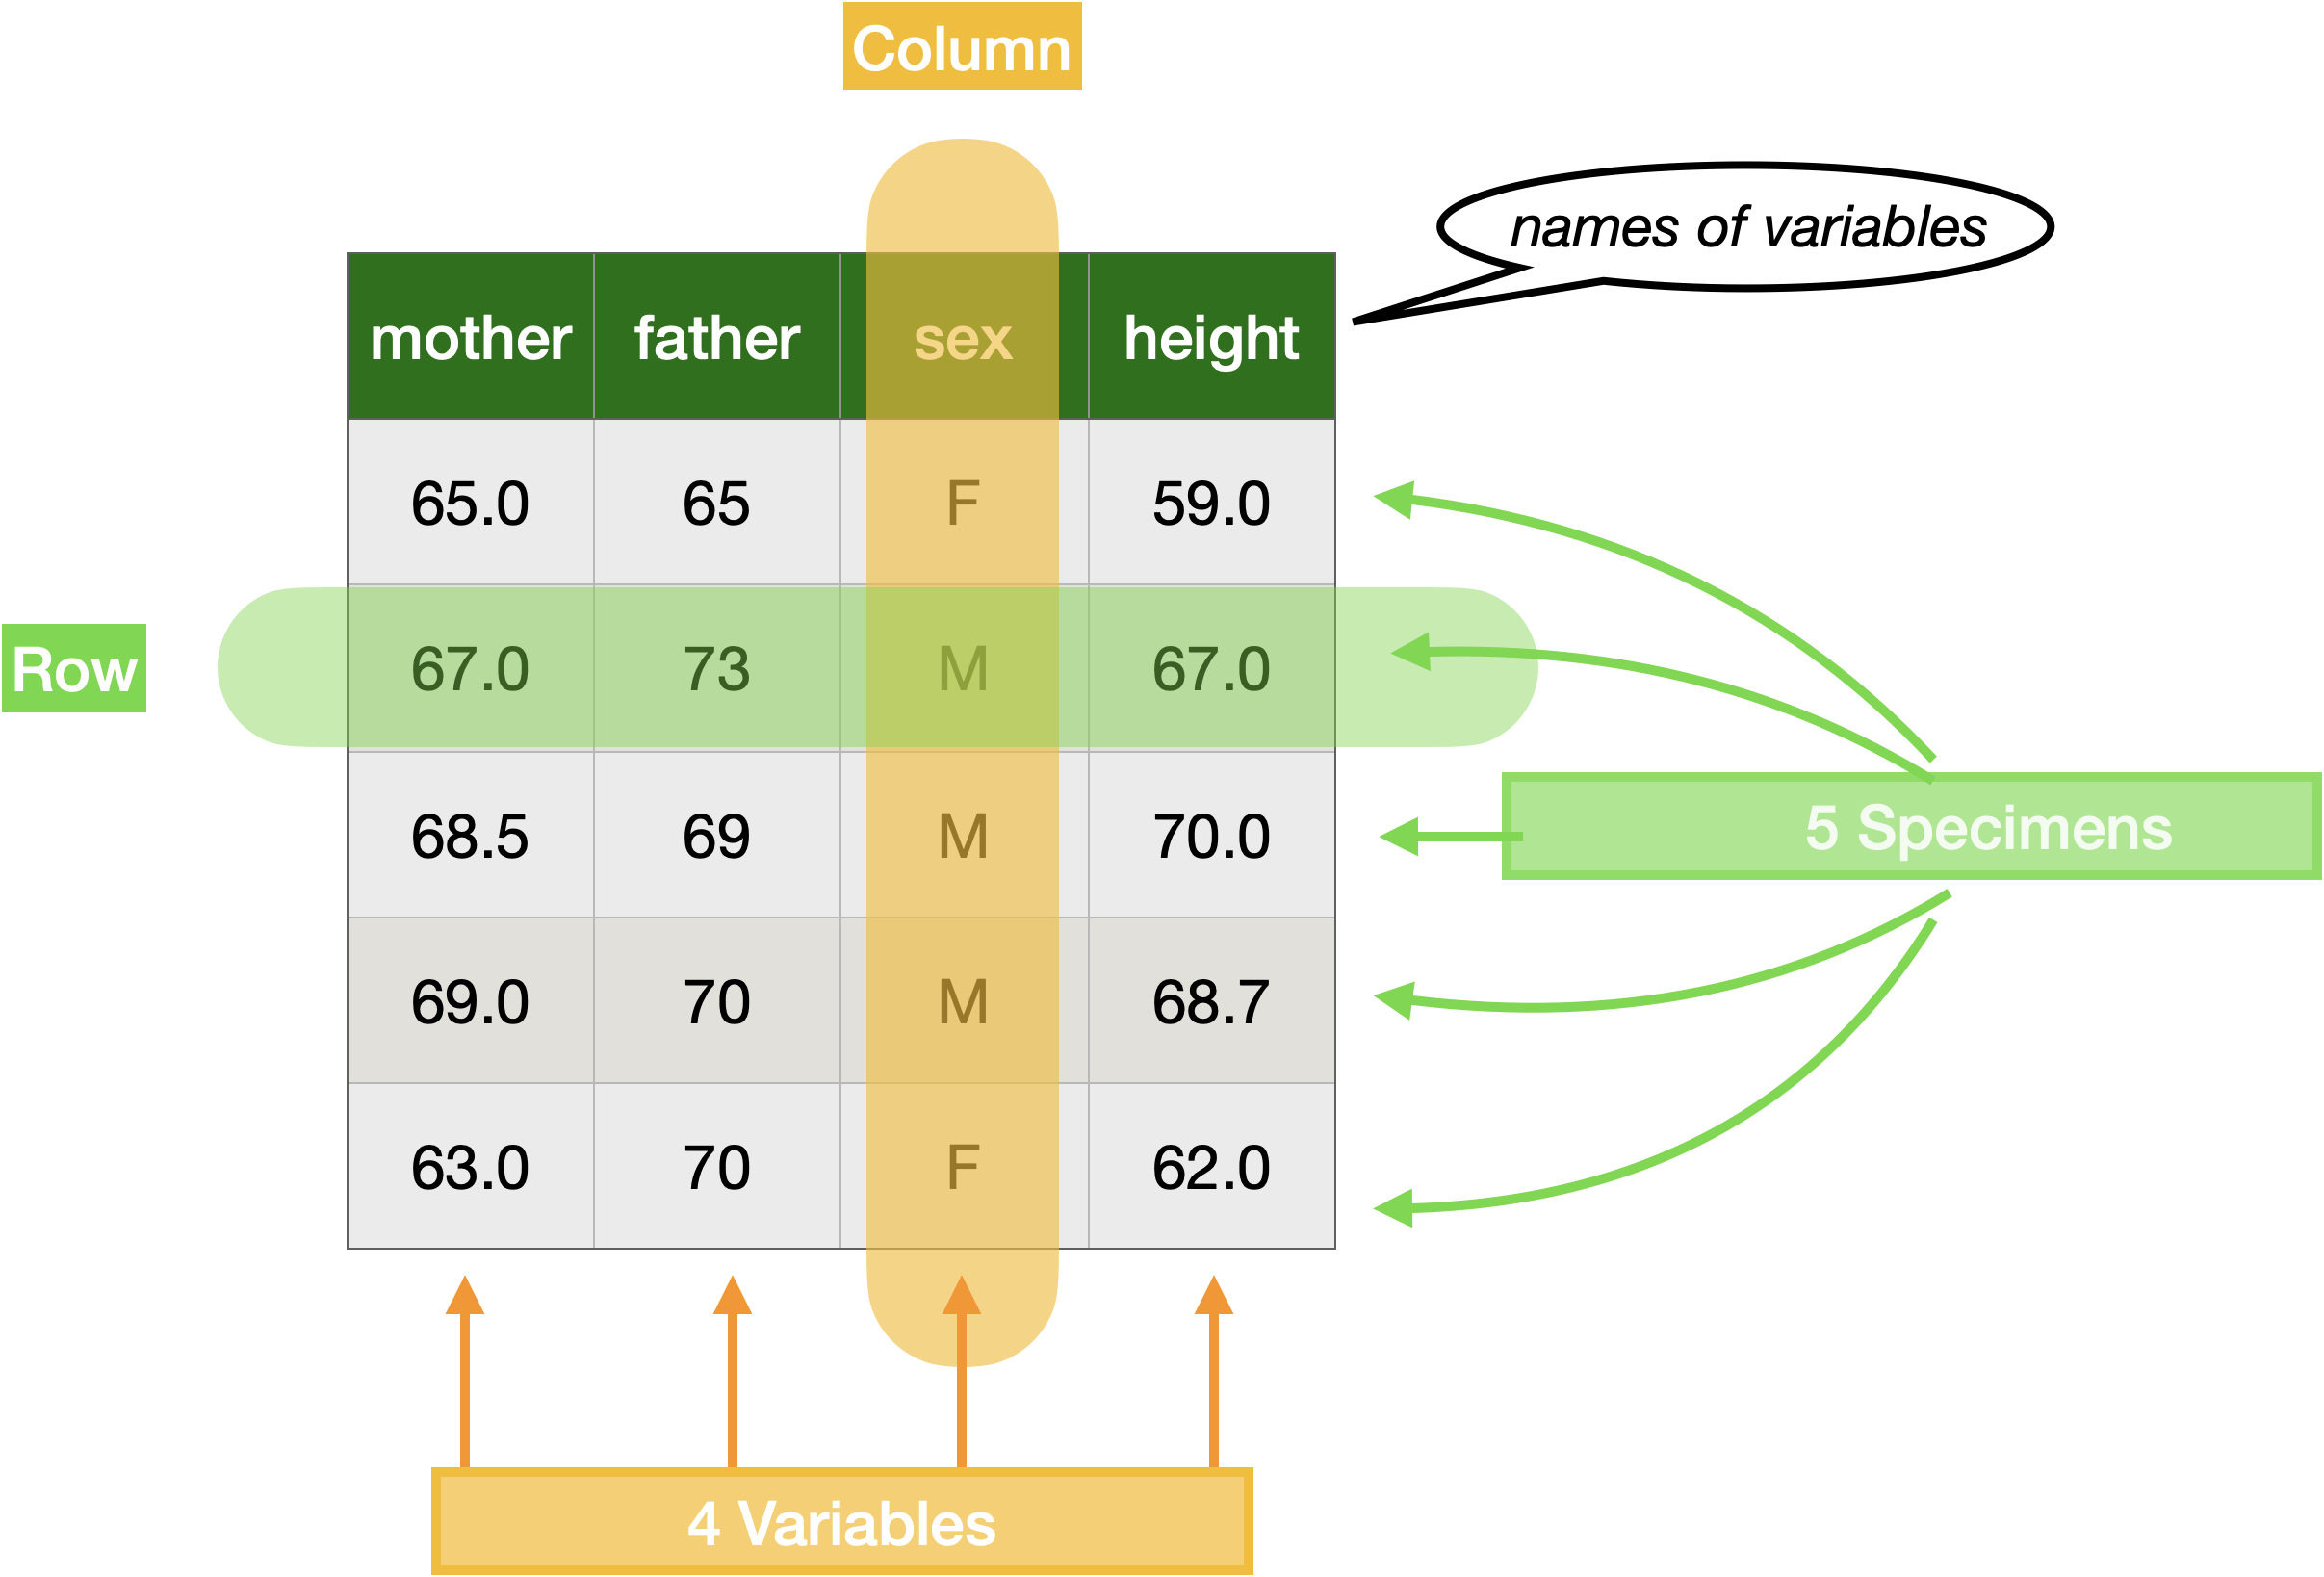
\includegraphics[width=8.05in,height=\textheight]{www/data-frame-schematic.png}

}

\end{figure}%

The row-and-column organization of a data frame is reminiscent of a
spreadsheet. However, data frames have additional organizational
requirements that typical spreadsheet software does not enforce. The
term ``\textbf{tidy data}'' emphasizes that these requirements are being
met.

\begin{enumerate}
\def\labelenumi{\arabic{enumi}.}
\item
  Each variable must consist of the same kind of individual entries. For
  example, the \texttt{mother} variable consists of numbers: a quantity.
  In this case, the quantity is the mother's height in inches. It would
  not be legitimate for an entry in \texttt{mother} to be a word or to
  be a height in meters or something else entirely, for instance, a
  blood pressure.
\item
  Each row represents an individual real-world entity. For the data
  frame shown in Figure~\ref{fig-data-frame-schematic}, each row
  corresponds to an individual, fully-grown child. We use the term
  ``\textbf{unit of observation}'' to refer to the \emph{kind of entity}
  represented in each row. All rows in a data frame must be the same
  kind of unit of observation. It would not be legitimate for some rows
  to individual people while others refer to something different such as
  a house or family or country. If you wanted to record data on
  families, you would need to create a new data frame where the unit of
  observation is a family.
\end{enumerate}

We use the word ``\textbf{specimen}'' to refer to an individual instance
of the unit of observation. A data frame is a collection of specimens.
Each row represents a unique specimen.

The unit of observation in Figure~\ref{fig-data-frame-schematic} is a
full-grown child. The fifth row in that data frame refers to a unique
young woman in London in the 1880s (whose name is lost to history). By
using the word ``specimen'' to refer to this woman, we do not mean to
dehumanize her. However, we need a phrase that can be applied to a
single row of any data frame, whatever its unit of observation might be:
a shipping container, a blood sample, a day of ticket sales, and so on.

The collection of specimens comprised by a data frame is often a
``\textbf{sample}'' from a larger group of the units of observation.
Galton did not measure the height of every fully-grown child in London,
England, the UK, or the World. He collected a \emph{sample} from London
families. Sometimes, a data frame includes every possible instance of
the unit of observation. For example, a library catalog lists
comprehensively the books in a library. Such a comprehensive collection
is called a ``\textbf{census}.''

\begin{tcolorbox}[enhanced jigsaw, colbacktitle=quarto-callout-note-color!10!white, opacityback=0, breakable, opacitybacktitle=0.6, colback=white, coltitle=black, arc=.35mm, title=\textcolor{quarto-callout-note-color}{\faInfo}\hspace{0.5em}{Example: New-born babies}, left=2mm, colframe=quarto-callout-note-color-frame, rightrule=.15mm, bottomrule=.15mm, leftrule=.75mm, bottomtitle=1mm, toptitle=1mm, titlerule=0mm, toprule=.15mm]

The US Centers for Disease Control (CDC) publishes a ``public use file''
each year, a data frame where the unit of observation is an infant born
in the US. (The many variables include the baby's weight and sex, the
mother's age, and the number of prenatal care visits during the
pregnancy.) The published file for 2022 contains 3,699,040 rows; that is
the number of (known) births in 2022. As such, the CDC data constitutes
a \textbf{census} rather than a \textbf{sample}.

\end{tcolorbox}

\subsection{Types of variables}\label{types-of-variables}

Each column of a data frame is a variable. The word ``variable'' is
appropriate because the entries within a variable \textbf{vary} one from
one row to another. Other words with the same root include
``variation,'' ``variety,'' and even ``diversity.''

Data-frame variables come in two fundamental types:

{\marginnote{\begin{footnotesize}The distinction between quantitative
and categorical variables is fundamental to statistical work. You should
be able to discern whether a variable is categorical or quantitative
from a glance at a data frame.\end{footnotesize}}}

\begin{enumerate}
\def\labelenumi{\arabic{enumi}.}
\item
  \textbf{Quantitative} variables record an ``amount'' of something.
  These might just as well be called ``numerical'' variables.
\item
  \textbf{Categorical} variables typically consist of letters. For
  instance, the \texttt{sex} variable in
  Figure~\ref{fig-data-frame-schematic} contains entries that are either
  \textbf{F} or \textbf{M}. In most of the data we work with in these
  \emph{Lessons}, there is a fixed set of entry values called the
  \textbf{levels} of the categorical variable. The levels of
  \texttt{sex} are \textbf{F} and \textbf{M}.
\end{enumerate}

{\marginnote{\begin{footnotesize}We are not doing full justice to the
variety of possible variable types by focusing on just two type:
quantitative and categorical. You should be aware that there are other
kinds, for example, photographs or dates.\end{footnotesize}}}

\begin{tcolorbox}[enhanced jigsaw, colbacktitle=quarto-callout-note-color!10!white, opacityback=0, breakable, opacitybacktitle=0.6, colback=white, coltitle=black, arc=.35mm, title=\textcolor{quarto-callout-note-color}{\faInfo}\hspace{0.5em}{Example (cont.): The CDC births data frame}, left=2mm, colframe=quarto-callout-note-color-frame, rightrule=.15mm, bottomrule=.15mm, leftrule=.75mm, bottomtitle=1mm, toptitle=1mm, titlerule=0mm, toprule=.15mm]

Among the many variables in the CDC public use file of births are
\texttt{place} and \texttt{diabetes\_gest}, which record the place of
birth and whether the mother developed gestational diabetes.

The \texttt{place} variable is categorical, with these levels:

\begin{itemize}
\tightlist
\item
  ``hospital''
\item
  ``home (intended)''
\item
  ``home (unintended)''
\item
  ``freestanding''
\item
  ``other''
\end{itemize}

The \texttt{diabetes\_gest} variable has two levels: \textbf{N} or
\textbf{Y}.

\end{tcolorbox}

\subsection{The codebook}\label{sec-codebook}

How are you to know for any given data frame what constitutes the unit
of observation or what each variable is about? This information,
sometimes called \textbf{metadata}, is stored outside the data frame.
Often, the metadata is contained in a separate documentation file called
a ``\textbf{codebook}.''

To start, the codebook should make clear what is the unit of observation
for the data frame. For instance, we described the unit of observation
for the data frame shown in Figure~\ref{fig-data-frame-schematic} as a
fully grown child. This detail is important. For instance, each such
child---each specimen---can appear only once in the data frame. In
contrast, the same \texttt{mother} and \texttt{father} might appear for
multiple specimens, namely, the siblings of the child.

In the CDC data frame, the unit of observation is a newborn baby. If a
birth resulted in twins, each of the two babies will have its own row.
In contrast, imagine a data frame for the birth mothers or another for
prenatal care visits. Each mother could appear only once in the
birth-mothers frame, but the same mother can appear multiple times in
the prenatal care data frame.

For quantitative variables, the relevant metadata includes what the
number refers to (e.g., mother's height or baby's weight) and the
physical units of that quantity (e.g., inches for height or grams for
weight).

For categorical variables, the metadata should describe the meaning of
each level in as much detail as necessary.

\begin{tcolorbox}[enhanced jigsaw, colbacktitle=quarto-callout-note-color!10!white, opacityback=0, breakable, opacitybacktitle=0.6, colback=white, coltitle=black, arc=.35mm, title=\textcolor{quarto-callout-note-color}{\faInfo}\hspace{0.5em}{Example (cont.): CDC births codebook}, left=2mm, colframe=quarto-callout-note-color-frame, rightrule=.15mm, bottomrule=.15mm, leftrule=.75mm, bottomtitle=1mm, toptitle=1mm, titlerule=0mm, toprule=.15mm]

The codebook for the CDC data is a PDF document entitled ``User Guide to
the 2022 Natality Public Use File.'' You can access it on the
\href{https://ftp.cdc.gov/pub/Health_Statistics/NCHS/Dataset_Documentation/DVS/natality/UserGuide2022.pdf}{CDC
website}.

\end{tcolorbox}

\subsection{Accessing data frames}\label{accessing-data-frames}

Most statistics software, including R, makes it easy to access data
frames stored as files in any of a variety of formats. (For examples,
see Exercise 1.18.)

Almost all the data frames used as examples or exercises in these
\emph{Lessons} are stored in files provided by R software
``\textbf{packages}'' such as \texttt{\{LSTbook\}} or
\texttt{\{mosaicData\}}. The data frame itself is easily accessed by a
simple name, e.g., \texttt{Galton}. The location of the data frame is
specified by the package name as a prefix followed by a pair of colons,
e.g.~\texttt{mosaicData::Galton}. A convenient feature of this system is
the easy access to documentation by giving a command consisting of a
question mark followed by the
\emph{package-name}::\emph{data-frame-name}, e.g.

\begin{Shaded}
\begin{Highlighting}[]
\NormalTok{?mosaicData}\SpecialCharTok{::}\NormalTok{Galton}
\end{Highlighting}
\end{Shaded}

\subsection{Computing with data frames}\label{sec-computing-data-frames}

Lessons \ref{sec-point_plots}, \ref{sec-variation-and-distribution} \&
\ref{sec-model-annotation} cover how to make informative graphics that
give an overview of the contents in a data frame. Lesson
\ref{sec-wrangling} introduces commands for manipulating the contents of
a data frame to put them in a more useful form for the data graphics or
data summary task at hand.

This Lesson shows you how to access data frames and their documentation
and how to perform simple tasks such as listing the variable names or
glimpsing a few rows of a data frame.

There are many software systems for working with data frames. Commonly
available spreadsheet software, while suited to some data-entry and
data-summarizing tasks, is surprisingly limited when it comes to
statistical thinking. The system we will use, RStudio, is one of a
handful used by data science professionals. It's available free both as
an online, browser-based platform and for installation on a laptop
computer or computer server.

Much of the statistical work you do in RStudio consists of writing
commands in the R language. The word ``language'' is offputting to many
people, associating it as they do with natural languages such as Chinese
or Spanish, mastery of which takes time and much work. Fortunately, you
do not have to learn the R language; you need only a couple dozen R
expressions to work through all these \emph{Lessons}.

\marginnote{\begin{footnotesize}

If you are on your own, the instructions below provide a quick way to
get started with minimal effort.

If you are a student using these Lessons as part of a class, check with
your instructor who may already have set up a way for you to access
RStudio.

\end{footnotesize}}

We continue here under the assumption that you have already been shown
how to install and access RStudio by an instructor or other mentor. That
person will have arranged to install some additional software written
for these \emph{Lessons}, particularly the \texttt{\{LSTbook\}} package.

Each time you open RStudio, load the \texttt{\{LSTbook\}} package using
this \textbf{command} at the R prompt in the ``console'' tab.

\begin{Shaded}
\begin{Highlighting}[]
\FunctionTok{library}\NormalTok{(LSTbook)}
\end{Highlighting}
\end{Shaded}

\begin{tcolorbox}[enhanced jigsaw, colbacktitle=quarto-callout-note-color!10!white, opacityback=0, breakable, opacitybacktitle=0.6, colback=white, coltitle=black, arc=.35mm, title=\textcolor{quarto-callout-note-color}{\faInfo}\hspace{0.5em}{Starting out with R via \texttt{posit.cloud}}, left=2mm, colframe=quarto-callout-note-color-frame, rightrule=.15mm, bottomrule=.15mm, leftrule=.75mm, bottomtitle=1mm, toptitle=1mm, titlerule=0mm, toprule=.15mm]

Note: Otherwise \ldots{}

\texttt{posit.cloud} is a ``freemium'' web service. The word
``freemium'' signals that you can use it for free, up to a point.
Fortunately, that point will suffice for you to follow all of these
\emph{Lessons}.

\begin{enumerate}
\def\labelenumi{\arabic{enumi}.}
\tightlist
\item
  In your browser, follow
  \href{https://posit.cloud/content/6532153}{this link}. This will take
  you to \texttt{posit.cloud} and, after asking you to login via Google
  or to set up an account, will bring you to a page that will look much
  like the following. (It may take a few minutes.)
\end{enumerate}

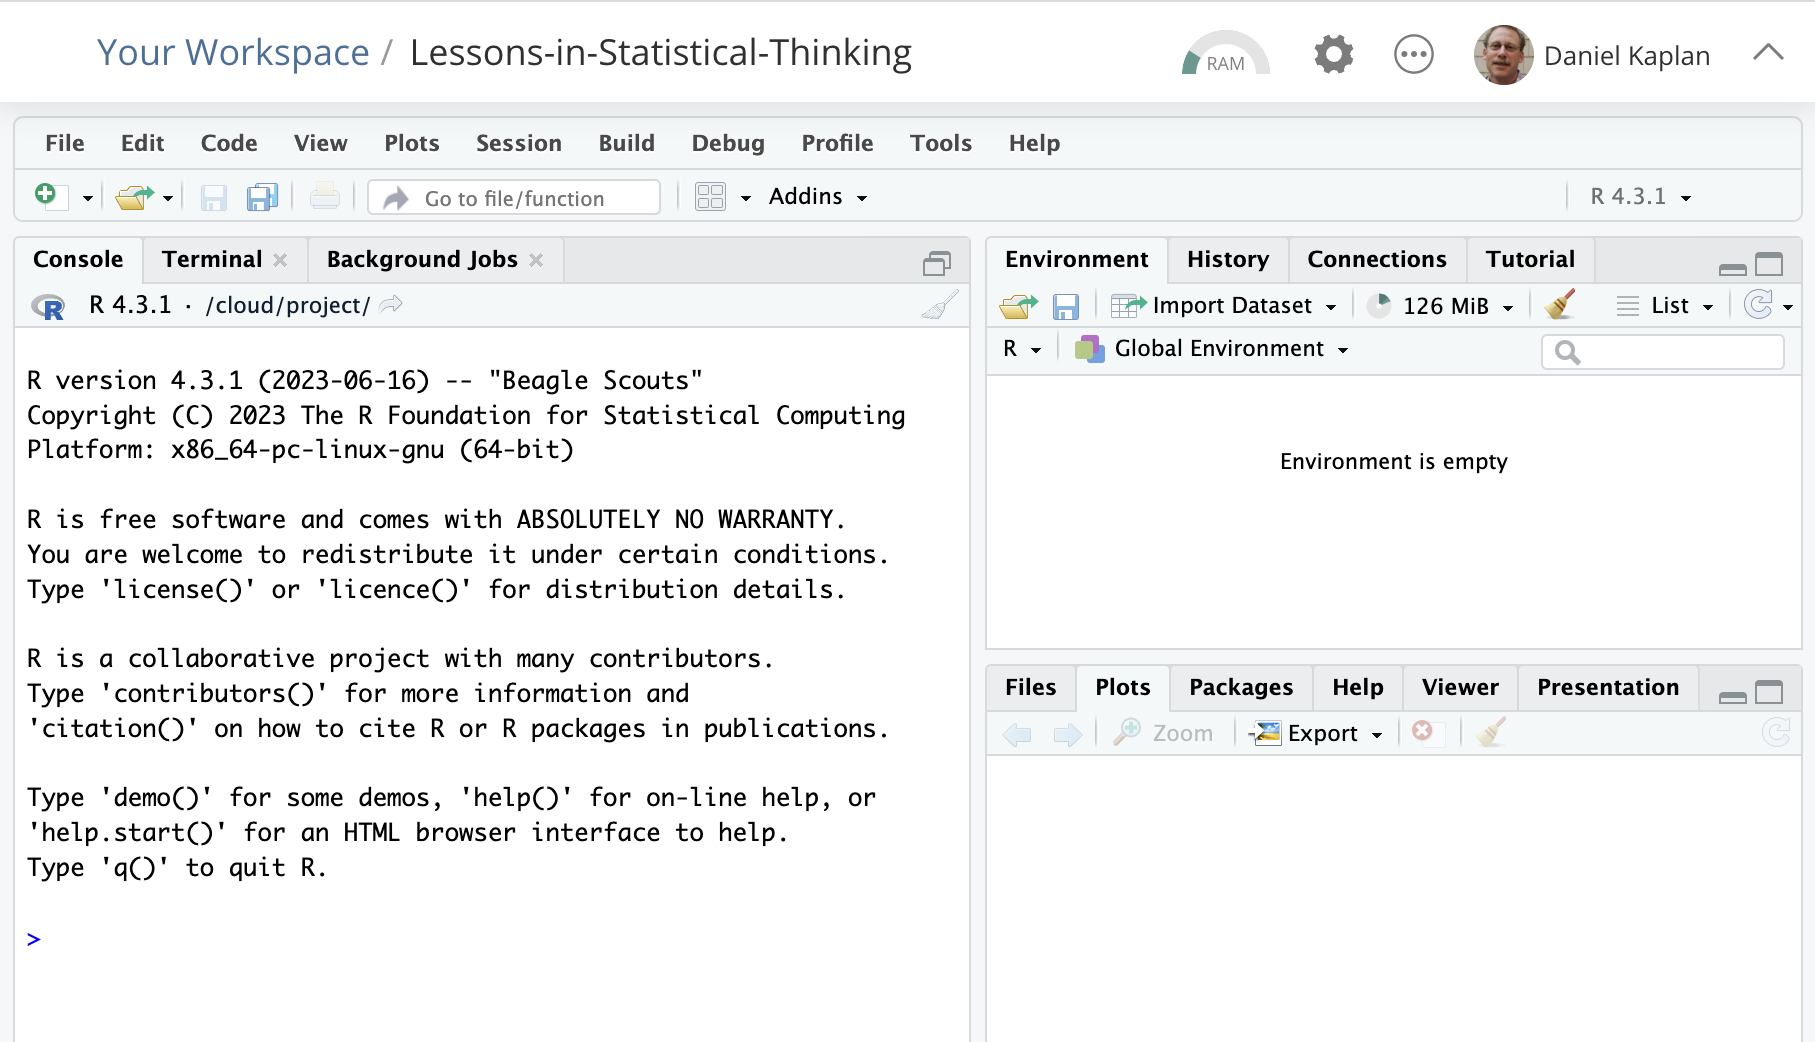
\includegraphics{www/posit-cloud.png}

\begin{enumerate}
\def\labelenumi{\arabic{enumi}.}
\setcounter{enumi}{1}
\item
  On the left half of the window, there are three ``tabs'' labelled
  ``Console,'' ``Terminal,'' and ``Background Jobs.'' You will be
  working in the ``Console'' tab. Click in that tab and you will see a
  flashing \texttt{\textbar{}} cursor after the \texttt{\textgreater{}}
  sign.
\item
  Give this command, exactly as written, and press return: ::: \{.cell\}
\end{enumerate}

\begin{Shaded}
\begin{Highlighting}[]
\FunctionTok{library}\NormalTok{(LSTbook)}
\end{Highlighting}
\end{Shaded}

\end{tcolorbox}

Now you are ready to go. :::

All of your work with R will consist of giving commands at the
\texttt{\textgreater{}} prompt and pressing return. Possibly the
simplest of all commands is merely the name of a data frame. For
instance, the \texttt{\{LSTbook\}} package provides, among many others,
a data frame named \texttt{AAUP}. Try this as a command:

\begin{Shaded}
\begin{Highlighting}[]
\NormalTok{AAUP}
\end{Highlighting}
\end{Shaded}

The result of such a command will be a print-out of the first several
rows and columns of the data frame. Some of the data frames provided by
\texttt{\{LSTbook\}} have a couple of dozen rows, others have tens of
thousands. Printing out the first few rows of a data frame is useful
since it shows the variable names and you can see whether each variable
is quantitative or categorical.

To see the codebook for a data frame, simply precede the name with the
\texttt{?} character, for instance:

\begin{Shaded}
\begin{Highlighting}[]
\NormalTok{?Births2022}
\end{Highlighting}
\end{Shaded}

\begin{marginfigure}

\centering{

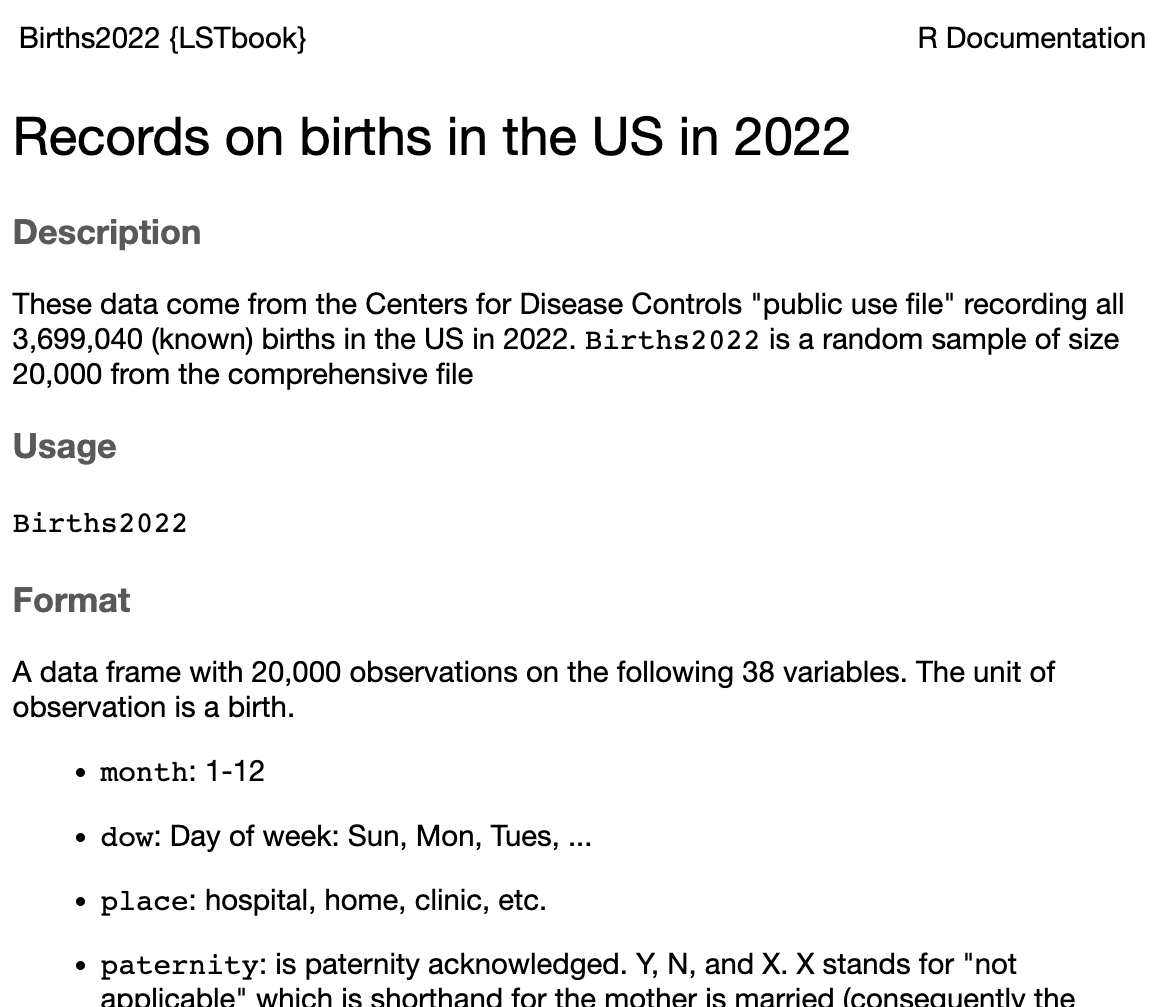
\includegraphics{www/births-documentation.png}

}

\caption{\label{fig-cdc-codebook}The codebook for the CDC births data
frame can be accessed with \texttt{?Births2022}. When displayed in the
RStudio Help tab, you can scroll through the descriptions of all 38
variables.}

\end{marginfigure}%

RStudio arranges for the codebook to be displayed in the ``Help'' tab.
This allows you to scroll through the documentation, follow web links
(if any), and keep the names of the variables displayed in the Help tab
while you write commands in the Console tab.

Commands you will use in these \emph{Lessons} will often start with the
name of a data frame followed a ``\textbf{pipeline} symbol
\texttt{\textbar{}\textgreater{}} which is then followed by a
description of the action you want to perform. Let's consider two simple
actions:

\begin{enumerate}
\def\labelenumi{\arabic{enumi}.}
\tightlist
\item
  Count the rows in the data frame:
\end{enumerate}

\begin{Shaded}
\begin{Highlighting}[]
\NormalTok{AAUP }\SpecialCharTok{|\textgreater{}} \FunctionTok{nrow}\NormalTok{()}
\end{Highlighting}
\end{Shaded}

\begin{verbatim}
[1] 28
\end{verbatim}

\begin{enumerate}
\def\labelenumi{\arabic{enumi}.}
\setcounter{enumi}{1}
\tightlist
\item
  List the names of the variables.
\end{enumerate}

\begin{Shaded}
\begin{Highlighting}[]
\NormalTok{AAUP }\SpecialCharTok{|\textgreater{}} \FunctionTok{names}\NormalTok{()}
\end{Highlighting}
\end{Shaded}

\begin{verbatim}
[1] "subject"  "acsal"    "fem"      "unemp"    "nonac"    "nonacsal" "licensed"
\end{verbatim}

These two commands have a similar structure involving four elements.

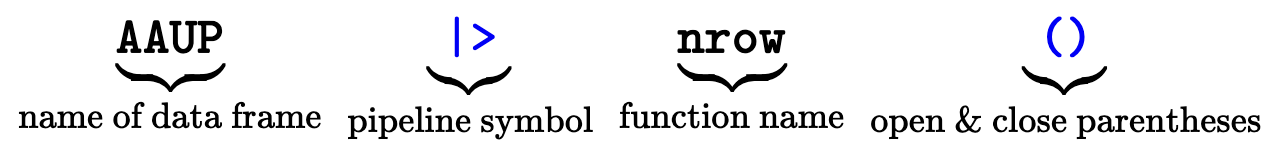
\includegraphics{www/latex-image-pipe.png}

There are two names in this command: the name of a data frame and a
``\textbf{function}'' name. The function name is how you specify what
you want to calculate from the data frame.

There are also two bits of punctuation:

\begin{itemize}
\item
  the pipeline symbol \texttt{\textbar{}\textgreater{}}, which connects
  the data frame to the function.
\item
  a pair of open and close parentheses immediately following the
  function name. Every time you use a function the function name will be
  followed by parentheses.
\end{itemize}

\begin{tcolorbox}[enhanced jigsaw, colbacktitle=quarto-callout-note-color!10!white, opacityback=0, breakable, opacitybacktitle=0.6, colback=white, coltitle=black, arc=.35mm, title=\textcolor{quarto-callout-note-color}{\faInfo}\hspace{0.5em}{Tables versus data frames}, left=2mm, colframe=quarto-callout-note-color-frame, rightrule=.15mm, bottomrule=.15mm, leftrule=.75mm, bottomtitle=1mm, toptitle=1mm, titlerule=0mm, toprule=.15mm]

You may notice that the displays of data frames printed in this book are
given labels such as Table~\ref{tbl-galton-dataframe}. It is natural to
wonder why the word ``table'' is used sometimes and ``data frame'' other
times.

In these \emph{Lessons} we make the following distinction. A ``data
frame'' stores values in the strict format of rows and columns described
previously. Data frames are ``machine readable.''

The data scientist working with data frames often seeks to create a
\textbf{display} intended for human eyes. A ``table'' is one kind of
\textbf{display} for humans. Since humans have common sense and have
learned many ways to communicate with other humans, a table does not
have to follow the restrictions placed on data frames. Tables are not
necessarily organized in strict row-column format, can include units for
numerical quantities and comments. An example is the table put together
by Francis Galton (Figure~\ref{fig-galton-notebook}) to organize his
measurements of heights.

\begin{figure}[H]

\sidecaption{\label{fig-galton-notebook}An excerpt from Francis Galton's
notebook recording the heights of parents and children in London in the
1880s.}

\centering{

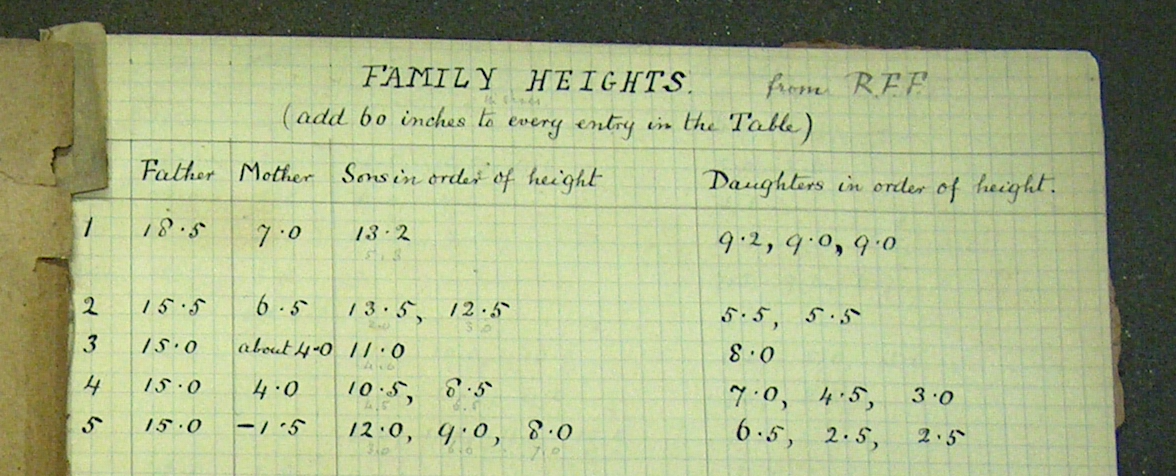
\includegraphics[width=3.92in,height=\textheight]{www/galton-notebook-excerpt.png}

}

\end{figure}%

We make the distinction between a data frame (for data storage) and a
table (for communicating with humans) because many of the operations
discussed in later lessons serve the purpose of transforming data frames
into human-facing displays such as graphics (Lesson
\ref{sec-point_plots}) or tables (Section~\ref{sec-displaying-tables}.)

Often, a literal display of a data frame may seem inefficient, for
instance this view of the \texttt{Galton} dataframe which was
constructed from Figure~\ref{fig-galton-notebook}.

\begin{Shaded}
\begin{Highlighting}[]
\NormalTok{Galton}
\end{Highlighting}
\end{Shaded}

\begin{table}[H]

\caption{\label{tbl-galton-dataframe}The records from the table shown in
Figure~\ref{fig-galton-notebook} in a data-frame format.}

\centering{

\begin{verbatim}


| family | father | mother | sex | height | nkids |
|:------:|:------:|:------:|:---:|:------:|:-----:|
|   1    |  78.5  |   67   |  M  |  73.2  |   4   |
|   1    |  78.5  |   67   |  F  |  69.2  |   4   |
|   1    |  78.5  |   67   |  F  |   69   |   4   |
|   1    |  78.5  |   67   |  F  |   69   |   4   |
|   2    |  75.5  |  66.5  |  M  |  73.5  |   4   |
|   2    |  75.5  |  66.5  |  M  |  72.5  |   4   |
|   2    |  75.5  |  66.5  |  F  |  65.5  |   4   |
|   2    |  75.5  |  66.5  |  F  |  65.5  |   4   |
|   3    |   75   |   64   |  M  |   71   |   2   |
|   3    |   75   |   64   |  F  |   68   |   2   |
\end{verbatim}

}

\end{table}%

It may seem that the data frame is inefficient, for example repeating
the heights of mother and father for all the siblings in a family. But
this view of efficiency relates to the use of paper and ink by a table;
the computer entity requires a different view of efficiency.

\end{tcolorbox}

\newpage

\section{Data graphics}\label{sec-point_plots}

The statistical thinker seeks to identify patterns in data, such as
possible relationships between variables. Translating a data frame into
graphical form---data graphics---is an important tool for revealing or
suggesting patterns.

\begin{figure}

\centering{

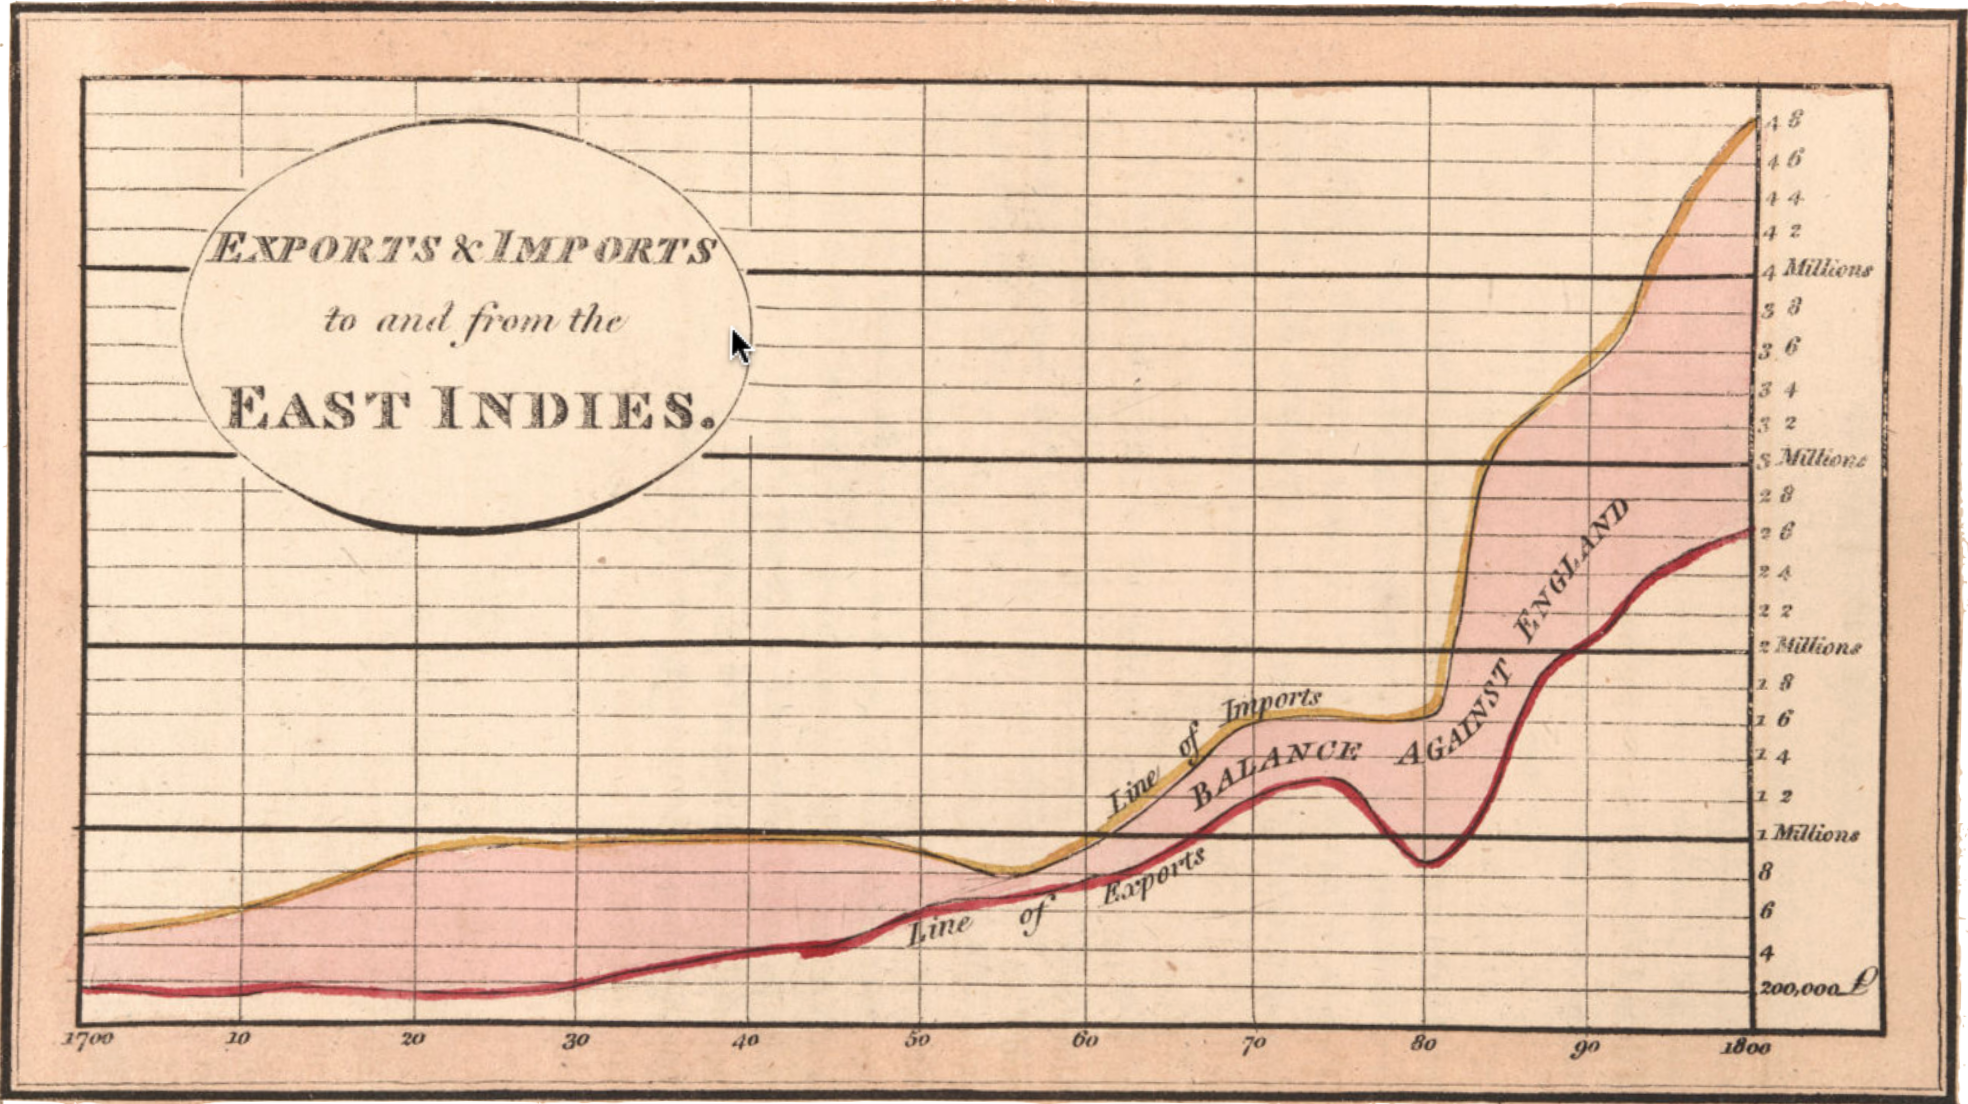
\includegraphics[width=6.56in,height=\textheight]{www/playfair-aligned.png}

}

\caption{\label{fig-playfair}William Playfair's 1801 presentation of
year-by-year data on trade between England and the East Indies.
\href{https://colenda.library.upenn.edu/catalog/81431-p3bv7bb8v}{Source:
University of Pennsylvania Libraries}}

\end{figure}%

\begin{marginfigure}

\caption{\label{tbl-playfair-trade}Annual exports and imports in the
trade between England and the East Indies}

\centering{

\begin{tabular}{r|r|r}
\hline
Year & Exports & Imports\\
\hline
1700 & 180 & 460\\
\hline
1701 & 170 & 480\\
\hline
1702 & 160 & 490\\
\hline
1703 & 150 & 500\\
\hline
1704 & 145 & 510\\
\hline
1705 & 140 & 525\\
\hline
1706 & 135 & 550\\
\hline
1707 & 125 & 565\\
\hline
1708 & 120 & 580\\
\hline
\end{tabular}

\emph{\ldots{} and so on to year 1800.}

}

\end{marginfigure}%

Making pictures of data is a relatively modern idea.
\href{https://en.wikipedia.org/wiki/William_Playfair}{William Playfair}
(1759-1823) is credited as the inventor of novel graphical forms in
which data values are presented graphically rather than as numbers or
text. To illustrate, consider the data from the 1700s
(Table~\ref{tbl-playfair-trade}) that Playfair turned into a picture.

Playfair's innovation, as in Figure~\ref{fig-playfair}, was successful
because it was powerful. A pattern that may be obscure in the data frame
becomes visually apparent to the human viewer. For example, consider the
graphic in Figure~\ref{fig-playfair} displaying data on trade between
England and the East Indies in the 1700s. The graphic lets you look up
the amount of trade each year, but it also shows patterns, such as the
upward \emph{trend} across the decades.

Data graphics can also make it easy to see deviations from trends, for
instance, the dip in exports and flattening of imports during 1775-1780.

Students often encounter various types of data graphics as they progress
through elementary and high school. Figure~\ref{fig-textbook-graphs}
shows a few examples commonly found in textbooks. Remarkably, it's rare
to encounter such textbook graphic types outside of a statistics course.

\begin{figure*}

\begin{minipage}{0.25\linewidth}

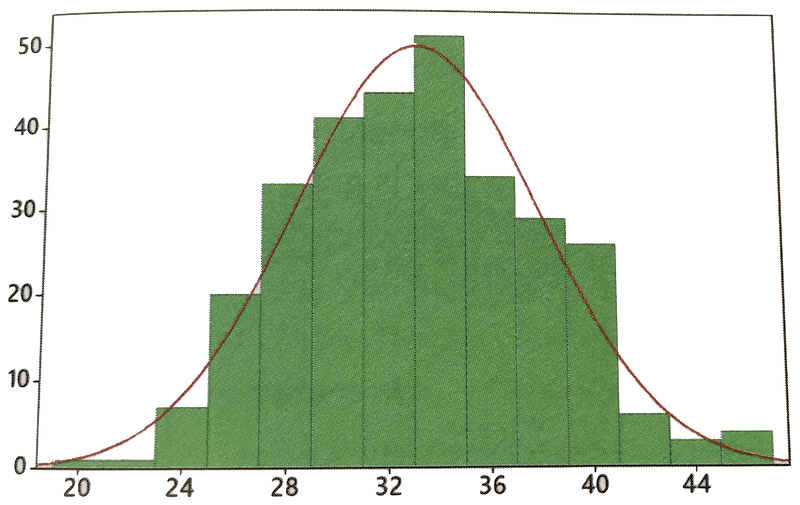
\includegraphics{www/thumbnail-hist2.png}

\subcaption{\label{}Histogram}
\end{minipage}%
%
\begin{minipage}{0.25\linewidth}

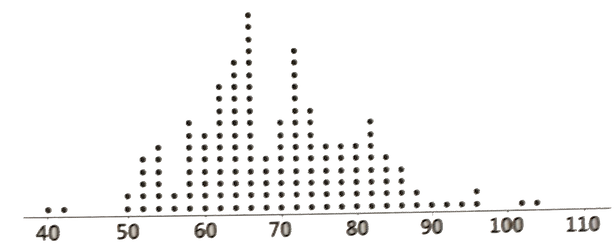
\includegraphics{www/thumbnail-dotplot.png}

\subcaption{\label{}Dot plot}
\end{minipage}%
%
\begin{minipage}{0.25\linewidth}

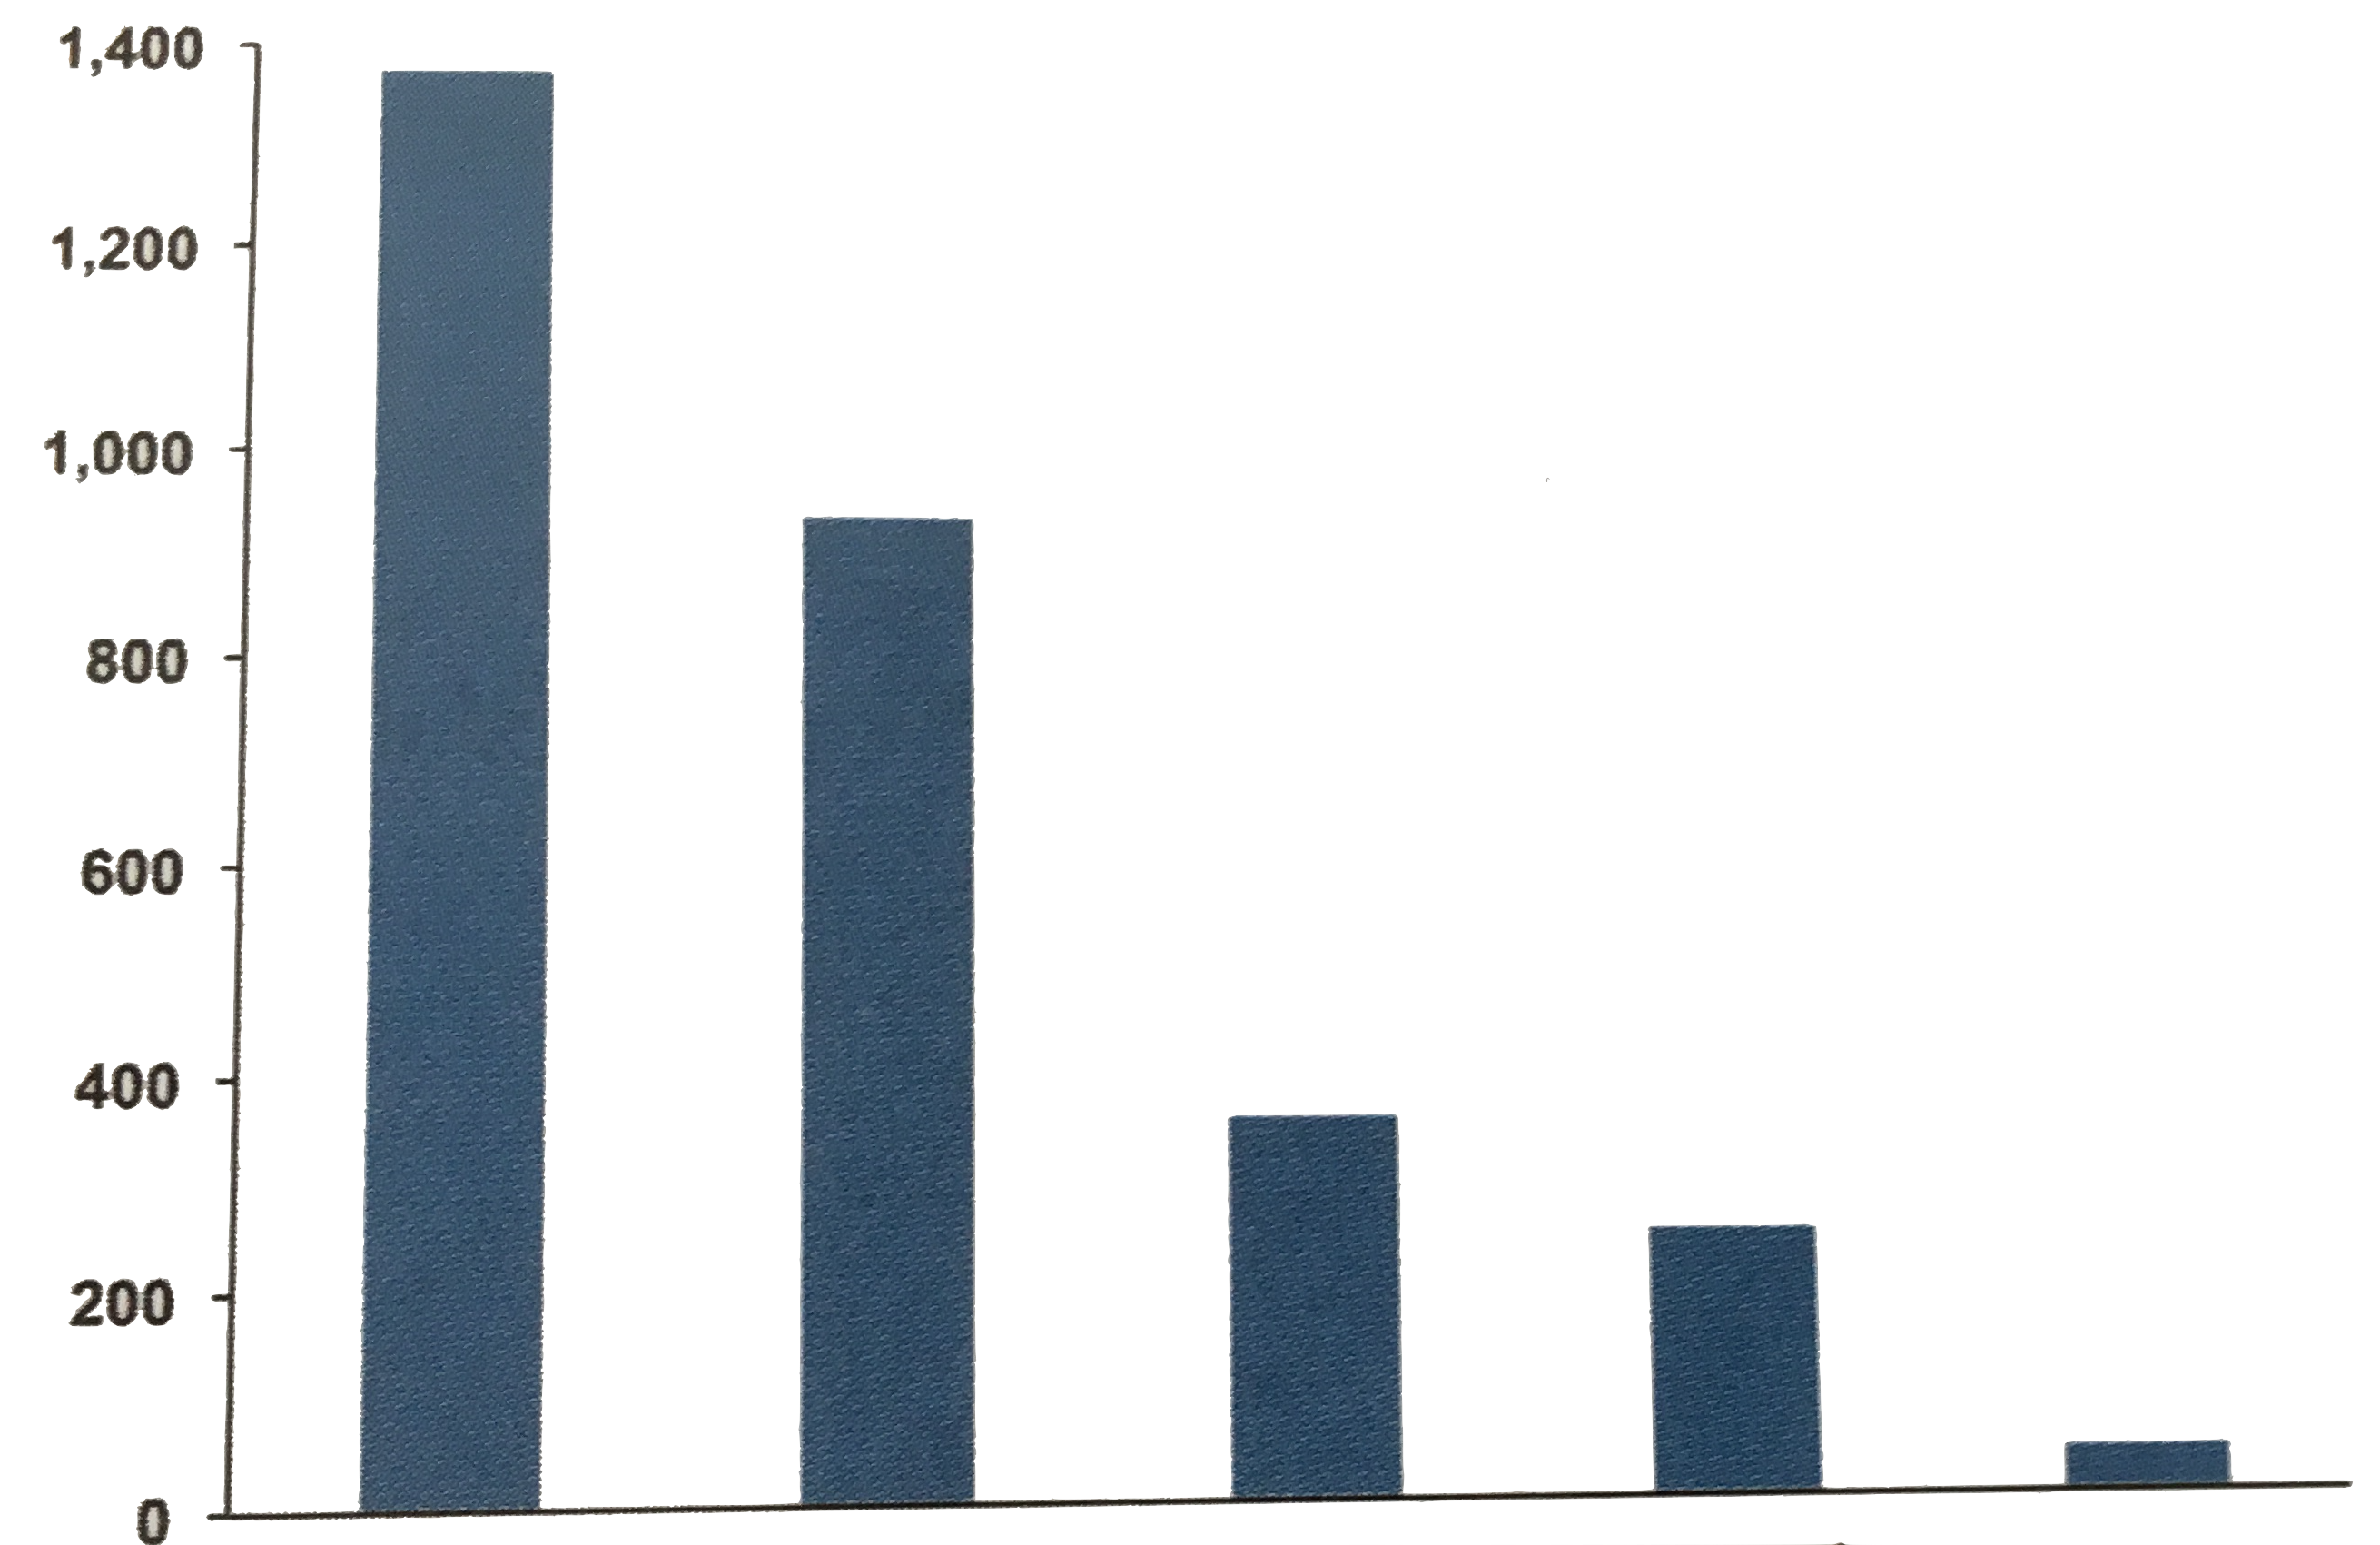
\includegraphics{www/thumbnail-barchart.png}

\subcaption{\label{}Bar chart}
\end{minipage}%
%
\begin{minipage}{0.25\linewidth}

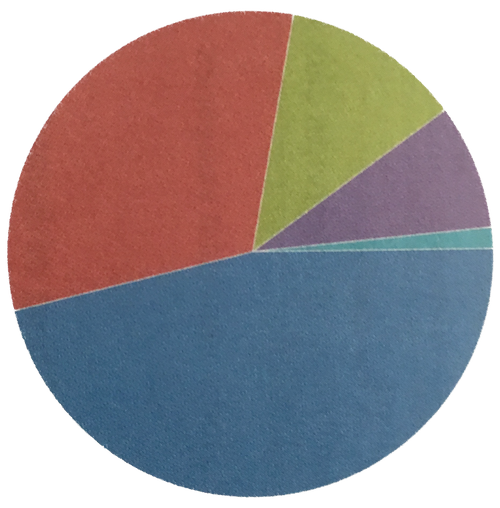
\includegraphics{www/thumbnail-pie.png}

\subcaption{\label{}Pie chart}
\end{minipage}%
\newline
\begin{minipage}{0.25\linewidth}

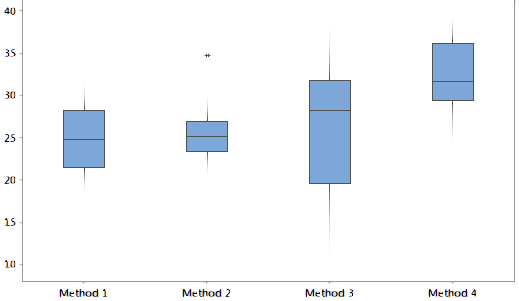
\includegraphics{www/thumbnail-boxplot.png}

\subcaption{\label{}Boxplot}
\end{minipage}%
%
\begin{minipage}{0.25\linewidth}

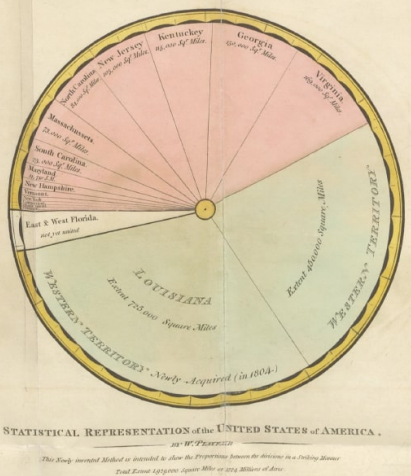
\includegraphics{www/playfair-pie-chart.png}

\subcaption{\label{}Playfair's pie chart}
\end{minipage}%
%
\begin{minipage}{0.25\linewidth}

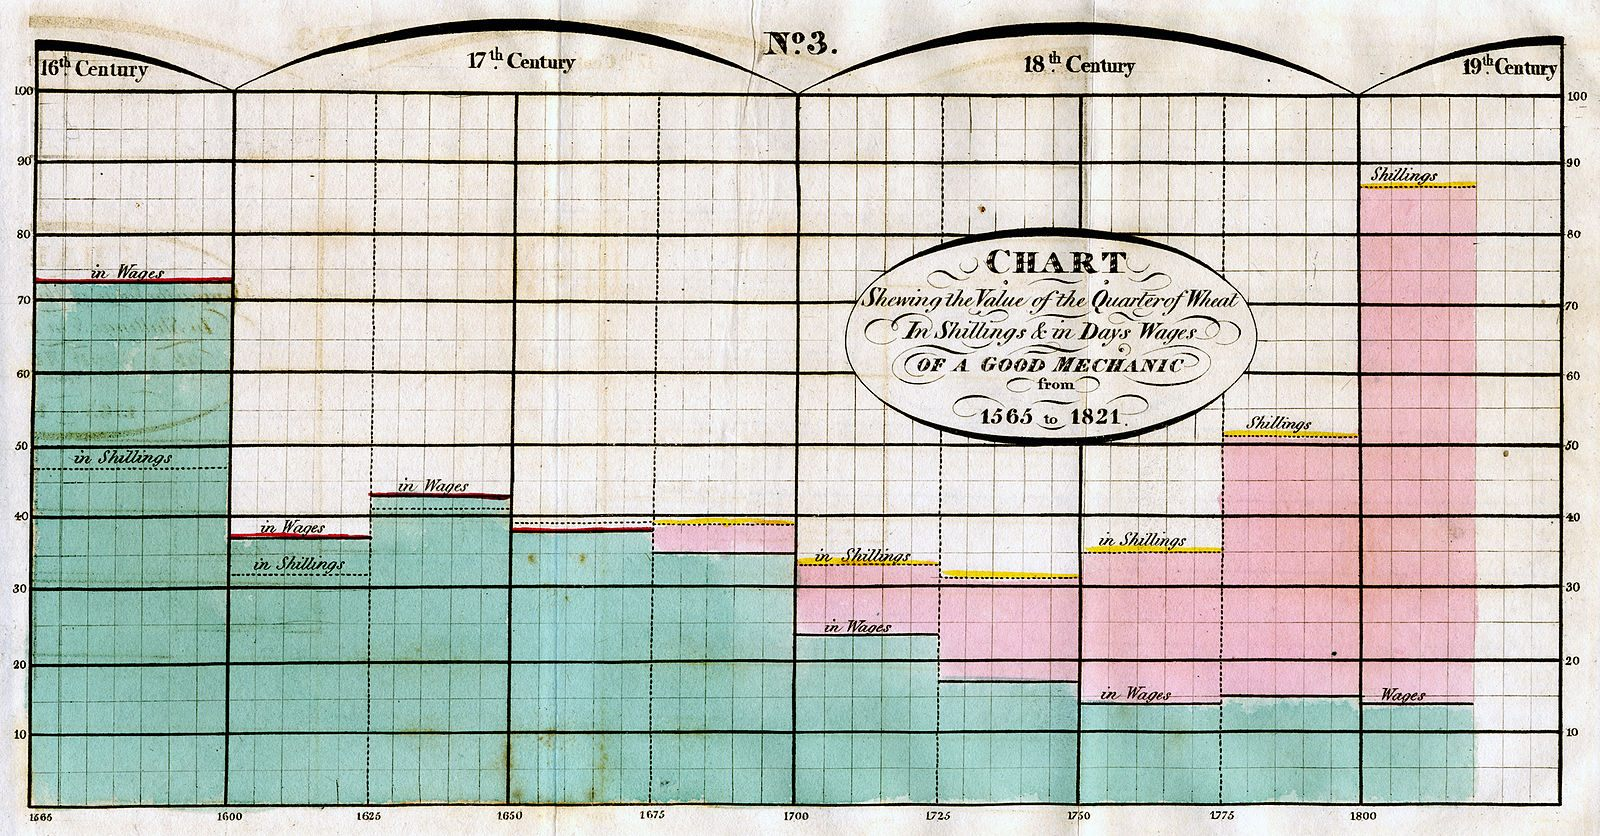
\includegraphics{www/playfair-barchart.png}

\subcaption{\label{}Playfairs bar chart}
\end{minipage}%
%
\begin{minipage}{0.25\linewidth}

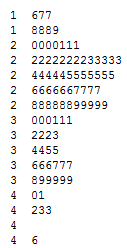
\includegraphics{www/thumbnail-stem-and-leaf.png}

\subcaption{\label{}Stem-and-leaf plot}
\end{minipage}%

\caption{\label{fig-textbook-graphs}Some of the graphics styles often
featured in statistics textbooks.}

\end{figure*}%

Modern data graphic designers are introducing even more variety; their
graphics can be captivating, colorful, dynamic, and informative. Some
online examples:
\href{https://flowingdata.com/2015/12/15/a-day-in-the-life-of-americans}{how
people spend their day},
\href{https://flowingdata.com/2017/01/24/one-dataset-visualized-25-ways}{life
expectancy}, \href{http://hint.fm/wind/}{wind patterns (right now!)},
\href{https://archive.nytimes.com/www.nytimes.com/imagepages/2011/11/06/opinion/06atrocities_timeline.html?action=click&contentCollection=Opinion&module=RelatedCoverage\%25C2\%25AEion=EndOfArticle&pgtype=article}{historical
sources of death}. The graphical types in
Figure~\ref{fig-textbook-graphs} were all invented long before computers
became available to help us work with data.

We won't use such graphical variety in these \emph{Lessons}.
{\marginnote{\begin{footnotesize}\href{Streamlining_graphics}{Note to
instructors}\end{footnotesize}}} Instead, we will use a single basic
form of graphic---the ``\textbf{annotated point plot}''---capable of
displaying multiple variables simultaneously and which can combine into
one view both the raw data and a summary of the patterns found in the
data.

\subsection{Point plot}\label{point-plot}

A \textbf{point plot} contains a simple mark---a dot---for each row of a
data frame. In its most common form, a point plot displays two selected
variables from the data frame. One variable is depicted as the vertical
coordinate, and the other as the horizontal coordinate.
{\marginnote{\begin{footnotesize}A ``point plot'' is also known as a
``scatter plot.''\end{footnotesize}}}

To illustrate how a point plot relates to the underlying data frame,
consider Table~\ref{tbl-world-cities}, where the unit of observation is
a city. (The data frame is available in R as
\texttt{maps::world.cities}.)

\begin{table}

\caption{\label{tbl-world-cities}Basic data on cities in the
\texttt{maps::world.cities} data frame}

\centering{

\begin{tabular}{l|l|r|r|r|r}
\hline
name & country.etc & pop & lat & long & capital\\
\hline
Shanghai & China & 15017783 & 31.23 & 121.47 & 2\\
\hline
Bombay & India & 12883645 & 18.96 & 72.82 & 0\\
\hline
Karachi & Pakistan & 11969284 & 24.86 & 67.01 & 0\\
\hline
Buenos Aires & Argentina & 11595183 & -34.61 & -58.37 & 1\\
\hline
Delhi & India & 11215130 & 28.67 & 77.21 & 0\\
\hline
Manila & Philippines & 10546511 & 14.62 & 120.97 & 1\\
\hline
\end{tabular}

\emph{\ldots{} and so on for 10,000 cities}

}

\end{table}%

Since \texttt{world.cities} contains several variables, many possible
\emph{pairs} of variables could be shown in point-plot form. For
instance, suppose we choose the \texttt{lat} and \texttt{long}
variables, which specify each city's location in terms of latitude and
longitude. Figure~\ref{fig-world-cities} shows a point plot of latitude
\emph{versus} longitude for world cities. By convention, the word
``versus'' in the phrase ``latitude versus longitude'' marks the role of
each variable in the point plot: latitude on the vertical axis and
longitude on the horizontal axis.

\begin{figure}

\centering{

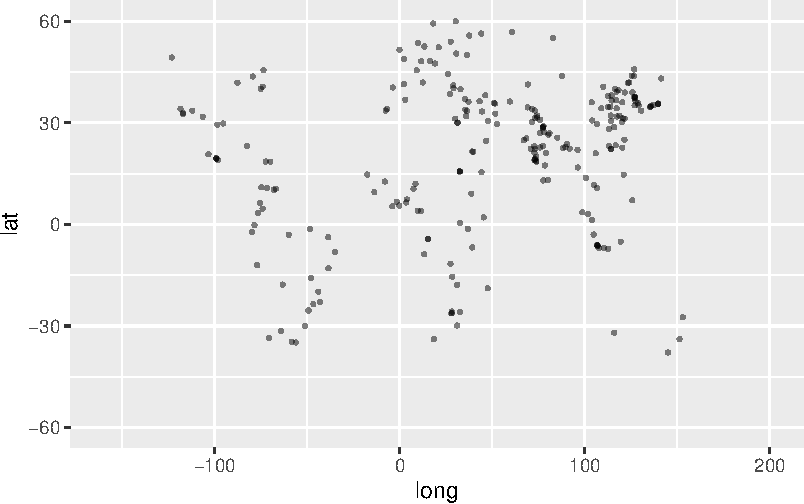
\includegraphics{test-tufte_files/figure-pdf/fig-world-cities-1.pdf}

}

\caption{\label{fig-world-cities}A point plot of the latitude versus
longitude of the world's 250 largest population cities.}

\end{figure}%

The dots in Figure~\ref{fig-world-cities} hint at some geographical
patterns you learned about in geography class. In general, the purpose
of a point plot is to hint at patterns in data.

To show how to construct a point plot, we will work with data on human
body shape. The \texttt{Anthro\_F} data frame records nineteen different
measurements of body shape for each of 184 college-aged women. (See
Table~\ref{tbl-wrist-ankle2})

\begin{table}

\caption{\label{tbl-wrist-ankle2}Some selected variables from the
\texttt{Anthro\_F} data frame.}

\centering{

\begin{tabular}{r|r|r|r|r|r|r|r}
\hline
Wrist & Ankle & Knee & Height & Neck & Biceps & Waist & BFat\\
\hline
18.4 & 23.5 & 37.5 & 1.6637 & 34.0 & 32.0 & 84.3 & 27.30\\
\hline
13.5 & 18.0 & 32.3 & 1.6002 & 27.1 & 23.2 & 60.2 & 17.62\\
\hline
18.0 & 22.5 & 38.5 & 1.6510 & 32.5 & 28.2 & 80.1 & 30.42\\
\hline
19.0 & 24.5 & 41.5 & 1.6637 & 35.0 & 34.5 & 90.0 & 34.24\\
\hline
\end{tabular}

}

\end{table}%

In making a point plot of \texttt{Anthro\_F}, we have to choose
\emph{two} variables to display. One variable will determine the
vertical position of the dots, the other variable will set the
horizontal position. For instance, in Figure~\ref{fig-wrist-ankle} we
choose \texttt{Wrist} for the vertical position and \texttt{Ankle} for
the horizontal position. In words, the plot is ``wrist \emph{versus}
ankle,'' that is, ``vertical \emph{versus} horizontal.'' (The codebook
for \texttt{Anthro\_F}---available via the R command
\texttt{?~Anthro\_F}---tells us that \texttt{Ankle} is measured as the
circumference in centimeters, and similarly for \texttt{Wrist}.)

\begin{Shaded}
\begin{Highlighting}[]
\NormalTok{Anthro\_F }\SpecialCharTok{|\textgreater{}} \FunctionTok{point\_plot}\NormalTok{(Wrist }\SpecialCharTok{\textasciitilde{}}\NormalTok{ Ankle)}
\end{Highlighting}
\end{Shaded}

\begin{figure}[H]

\centering{

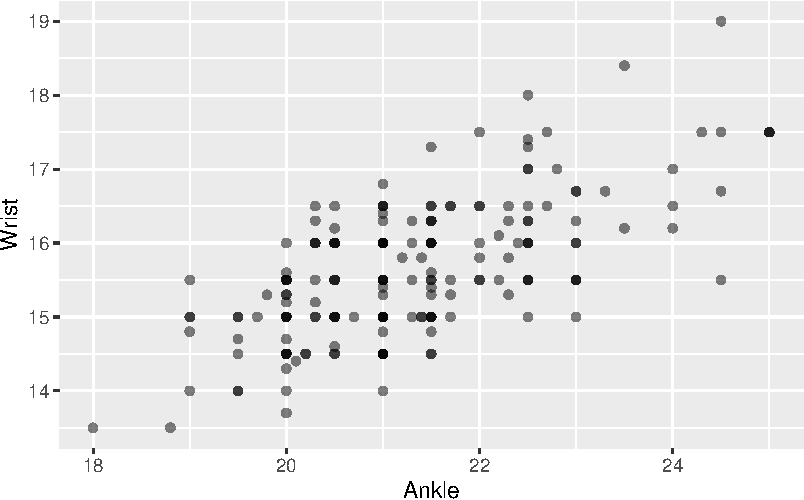
\includegraphics{test-tufte_files/figure-pdf/fig-wrist-ankle-1.pdf}

}

\caption{\label{fig-wrist-ankle}A point plot of wrist versus ankle
circumference.}

\end{figure}%

The pattern seen in Figure~\ref{fig-wrist-ankle} can be described as an
upward-sloping cloud. We will develop more formal descriptions of such
clouds in later Lessons. But for now, focus on the R command that
generated the point plot.

The point of an R command is to specify what action you want the
computer to take. Here, the desired action is to make a point plot based
on \texttt{Anthro\_F} using the two variables \texttt{Wrist} and
\texttt{Ankle}. Look carefully at the command for
Figure~\ref{fig-wrist-ankle}:

\texttt{Anthro\_F\ \textbar{}\textgreater{}\ point\_plot(Wrist\ \textasciitilde{}\ Ankle)}

The command includes all four of the names involved in the plot:

\begin{itemize}
\tightlist
\item
  The data frame \texttt{Anthro\_F}
\item
  The action \texttt{point\_plot}
\item
  The variables involved: \texttt{Wrist} and \texttt{Ankle}
\end{itemize}

These names are separated from one another by some punctuation marks:

\begin{itemize}
\tightlist
\item
  \texttt{\textbar{}\textgreater{}}, the ``pipe''
\item
  \texttt{()}, a pair of parentheses
\item
  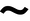
\includegraphics{www/tilde.png}, called ``tilde''
\end{itemize}

Don't be daunted by this punctuation, strange though it may seem at
first. You will get used to it, since almost all the commands you use in
these \emph{Lessons} will have the same punctuation.

Let's annotate the R command that made Figure~\ref{fig-wrist-ankle} to
identify the different components of the command:


\includegraphics{www/latex-image-point-plot.png}

Most commands in these \emph{Lessons} start with a data frame named at
the start of the command. This is followed by the pipe, which indicates
sending the data frame to the next command component. That next
component specifies which action to take. By convention,
``\textbf{Function}'' is used rather than ``action.'' You use
differently named functions to carry out different kinds of actions.
{\marginnote{\begin{footnotesize}You will need only a handful of
function for these \emph{Lessons}, for instance, \texttt{point\_plot},
\texttt{model\_train}, \texttt{conf\_interval()}, \texttt{mutate()},
\texttt{summarize()}.\end{footnotesize}}}

The function name is \emph{always} followed by an opening parenthesis.
Any details about what action to perform go between the opening and the
corresponding closing parentheses. In computer terminology, such details
are called ``\textbf{arguments}.'' The detail for the
Figure~\ref{fig-wrist-ankle} point\_plot is the choice of the two
variables to be used and which one goes on the vertical axis. This
detail is written as a ``\textbf{tilde expression}.'' The tilde
expression given as the argument to \texttt{point\_plot()} is
\texttt{Wrist\ \textasciitilde{}\ Ankle}, which can be pronounced as
``wrist \emph{versus} ankle'' or `wrist~\emph{tilde}~ankle,'' as you
prefer.

\subsection{Response and explanatory
variables}\label{response-and-explanatory-variables}

Another pronunciation for 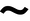
\includegraphics{www/tilde.png} is ``\ldots{}
as a function of \ldots.'' So, \texttt{Wrist~\textasciitilde{}~Ankle}
means ``wrist circumference as a function of ankle circumference.'' In
mathematics, functions are often written using a notation like \(f(x)\).
In this notation, \(x\) is the \textbf{input} to the function
\texttt{f()}. The word ``input'' is used in so many different contexts
that it's helpful to use other technical words to highlight the context.

\begin{itemize}
\item
  In \textbf{computer notation}, such as \texttt{f(x)} or
  \texttt{point\_plot(Wrist\ \textasciitilde{}\ Knee)}, an expression
  inside the parentheses is called an \textbf{argument}. In
  \texttt{f(x)}, the function is \texttt{f()} and the argument is
  \texttt{x}. In \texttt{point\_plot(Wrist\ \textasciitilde{}\ Knee)},
  the function is \texttt{point\_plot()} and the argument is the tilde
  expression \texttt{Wrist\ \textasciitilde{}\ Knee}.
\item
  In \textbf{statistics}, in the word phrase ``wrist circumference as a
  function of ankle circumference'' or, equivalently, the computer
  expression \texttt{Wrist\ \textasciitilde{}\ Knee} referring to the
  \texttt{Anthro\_F} data frame, we say that \texttt{Knee} is an
  \textbf{explanatory variable} and \texttt{Wrist} is the
  \textbf{response variable}. In graphics, such as
  Figure~\ref{fig-wrist-ankle}, convention dictates that the response
  variable is shown along the vertical axis and the explanatory is shown
  along the horizontal axis.
\end{itemize}

In Figure~\ref{fig-wrist-ankle}, why did we choose \texttt{Ankle} as the
explanatory variable and \texttt{Wrist} as the response variable for
this example? No particular reason. We could equally well have chosen
any of the \texttt{Anthro\_F} variables in either role, depending on our
interest. Typically, the statistical thinker will examine several
different pairs to gain an understanding of how the various variables
are related to one another.

\subsection{Categorical variables and
jittering}\label{categorical-variables-and-jittering}

In the previous example, the point\_plot of \texttt{Wrist} \emph{versus}
\texttt{Ankle}, both variables are \textbf{quantitative}: the respective
joints' circumference (in cm). point\_plots are also suited to
\textbf{categorical} variables. For example,
Figure~\ref{fig-mass-species} shows a pair of point plots made from the
\texttt{Penguins} data frame. The unit of observation is an individual
penguin. The selected explanatory variable, \texttt{species}, is
categorical. The response variable, \texttt{mass}, is quantitative.

\begin{figure*}

\centering{

\begin{figure*}[H]

\begin{minipage}{0.50\linewidth}

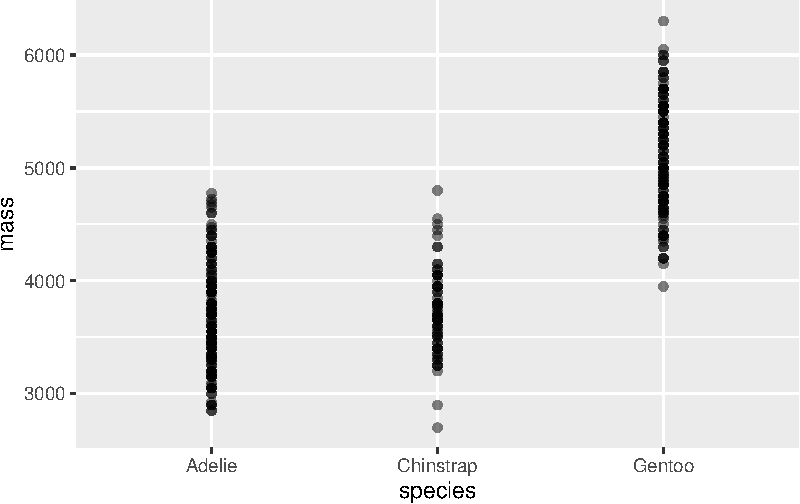
\includegraphics{test-tufte_files/figure-pdf/unnamed-chunk-48-1.pdf}

\subcaption{\label{}Without jittering}
\end{minipage}%
%
\begin{minipage}{0.50\linewidth}

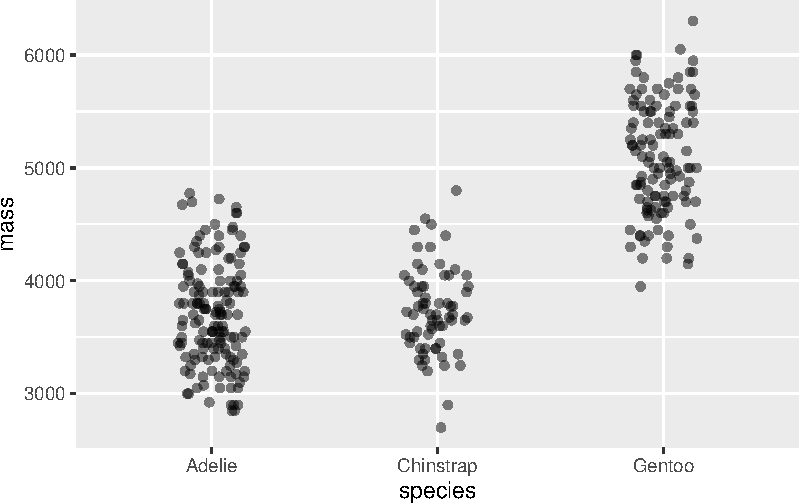
\includegraphics{test-tufte_files/figure-pdf/unnamed-chunk-48-2.pdf}

\subcaption{\label{}With jittering}
\end{minipage}%

\end{figure*}%

}

\caption{\label{fig-mass-species}The body mass of individuals of
different species of penguins.}

\end{figure*}%

When a categorical variable is used in a plot, the positions on the axis
are labelled with the levels of the variable. ``Adelie,'' ``Chinstrap,''
and ``Gentoo'' in the explanatory variable of
Figure~\ref{fig-mass-species}.

When an axis represent a \textbf{quantitative} variable, every possible
position on that axis refers to a specific value. For instance, the
Adelie penguins range between 2850 and 4775 grams. On the vertical axis
itself, marks are made at 3000 and 4000 grams, but we know that every
position in between those marks corresponds proportionately to a
specific numerical value.

In contrast, when an axis represents a \textbf{categorical} variable,
positions are marked for each level of that variable. But positions in
between marks are not referring to fictitious ``levels'' that do not
appear in the data. For instance, the position on the horizontal axis in
Figure~\ref{fig-mass-species} that's halfway between Adelie and
Chinstrap is \emph{not} reserved for individual penguins whose species
is a mixture of Adelie and Chinstrap; every value of a categorical
variables is one of the levels, which are discrete. There are no such
penguins! (Or, at least, the concept of ``species'' doesn't admit of
such.)

Using a coordinate axis to represent discrete categories makes common
sense, but we are left with the issue of interpreting the space between
those categories. In Figure~\ref{fig-mass-species} (left) the point plot
has been made ignoring the space between categories. Every specimen is
lined up directly above the corresponding level. The graphical result is
that it's hard to identify a single specimen since the dots are plotted
on top of one another..

``\textbf{Jittering}'' is a simple graphical technique that uses the
space between the levels to spread out the dots at random, as in
Figure~\ref{fig-mass-species} (right). This dramatically reduces overlap
and facilitates seeing the individual specimens. Recognize, however,
that the precise jittered position of a specimen does not carry
information about that specimen. All of the specimens in the column of
jittered dots above ``Adelie'' are the same with respect to species,
even though they may have different \texttt{mass}.

The \texttt{point\_plot()} function automatically uses jittering when
positioning in graphical space the values of categorical variables.

\subsection{Color and faceting}\label{color-and-faceting}

Often, there will be more than one explanatory variable of interest. A
penguins mass might not just be a matter of species; there are bigger
and smaller individuals within any species. Perhaps, for instance, the
body \emph{shape}---not just size---is different for the different
species. One way to investigate this possibility is to display body
\texttt{mass} as explained by \emph{both} species and, say,
\texttt{bill\_length}.

To specify that there are two explanatory variables, place their both
their names on the right-hand side of the tilde expression, separating
the names with a \texttt{+} or a \texttt{*}.
Figure~\ref{fig-mass-bill-species}(a) shows a point plot made with two
explanatory variables.

\begin{figure*}

\centering{

\begin{Shaded}
\begin{Highlighting}[]
\NormalTok{Penguins }\SpecialCharTok{|\textgreater{}} \FunctionTok{point\_plot}\NormalTok{(mass }\SpecialCharTok{\textasciitilde{}}\NormalTok{ bill\_length }\SpecialCharTok{+}\NormalTok{ species)}
\NormalTok{Penguins }\SpecialCharTok{|\textgreater{}} \FunctionTok{point\_plot}\NormalTok{(mass }\SpecialCharTok{\textasciitilde{}}\NormalTok{ bill\_length }\SpecialCharTok{+}\NormalTok{ species }\SpecialCharTok{+}\NormalTok{ sex)}
\end{Highlighting}
\end{Shaded}

\begin{figure*}[H]

\begin{minipage}{0.50\linewidth}

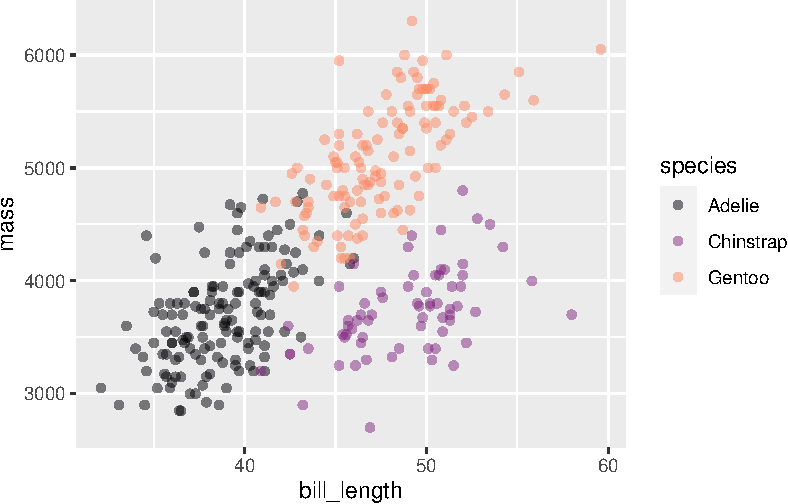
\includegraphics{test-tufte_files/figure-pdf/unnamed-chunk-49-1.pdf}

\subcaption{\label{}two explanatory variables}
\end{minipage}%
%
\begin{minipage}{0.50\linewidth}

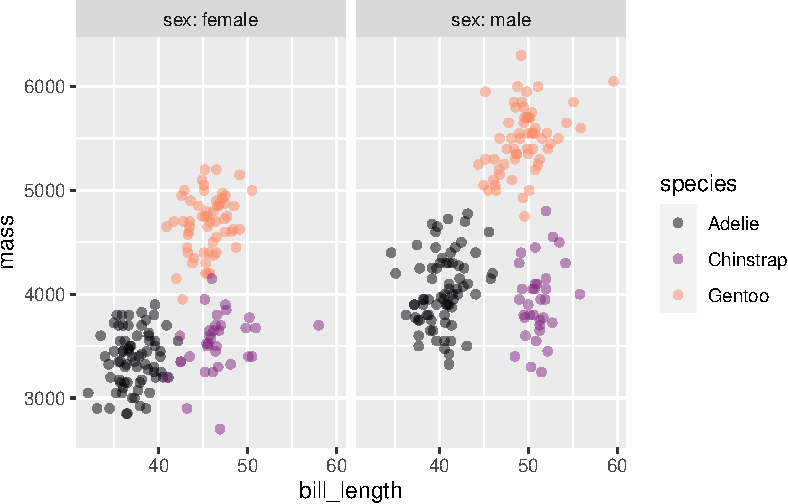
\includegraphics{test-tufte_files/figure-pdf/unnamed-chunk-49-2.pdf}

\subcaption{\label{}three explanatory variables}
\end{minipage}%

\end{figure*}%

}

\caption{\label{fig-mass-bill-species}Point plots involving multiple
explanatory variables.}

\end{figure*}%

Figure~\ref{fig-mass-bill-species}(b) involves three variables.
Consequently each dot has three different graphical attributes:

\begin{itemize}
\tightlist
\item
  position in space along the vertical axis. This is denoted as
  \textbf{y}.
\item
  position in space along the horizontal axis. This is denoted as
  \textbf{x}.
\item
  color, denoted, naturally enough, as \textbf{color}.
\end{itemize}

In order to avoid long-winded sentences involving phrases like ``the
horizontal axis represents \ldots.'' we use the word ``\textbf{mapped}.
For instance, in Figure~\ref{fig-mass-bill-species}, \texttt{mass} is
mapped to y, \texttt{bill\_length} is mapped to x, and \texttt{species}
is mapped to color. Each mapping has a \textbf{scale} that translates
the graphical property to a numerical or, in the case of color,
categorical value.

\texttt{point\_plot()} has been arranged so that the order of variable
names in the tilde expression argument,
\texttt{mass\ \textasciitilde{}\ bill\_length\ +\ species}, exactly
determines the mappings of variables to graphical properties. The
response variable---that is, the variable named on the left-hand side of
the tilde expression---is always mapped to y. The first variable on the
right-hand side---\texttt{bill\_length} in Figure
\ref{fig-mass-bill-species}---is always mapped to x. The second variable
named on the right-hand side is always mapped to color.

In Figure~\ref{fig-mass-bill-species}(right), four variables are shown:
the response \texttt{mass} as well as the three explanatory variables
\texttt{bill\_length}, \texttt{species}, and \texttt{sex}. Each variable
needs to be mapped to a unique graphical property.
\texttt{point\_plot()} maps the third explanatory variable (if any) to a
property called ``\textbf{facet}.'' Facets are drawn as separate
sub-panels. The scale for the mapping to facet consists of the labels at
the top of each facet.

With \texttt{point\_plot()}, different but closely related graphs of the
same data can be made by swapping the order of variables named in the
tilde expression. To illustrate, Figure~\ref{fig-mass-bill-species-sex2}
reverses the mappings \texttt{sex} and \texttt{species} compared to
Figure~\ref{fig-mass-bill-species}(b). The data are the same in the two
plots, but the different orderings of explanatory variables emphasize
different aspects of the relationship among the variables. For instance,
in \textbf{?@fig-mass-bill-species-sex}(b) it's easier to see that the
sexes of each species differ in both mass and bill length. Chinstrap
males and females have bill lengths that are the most distinct from one
another.

\begin{Shaded}
\begin{Highlighting}[]
\NormalTok{Penguins }\SpecialCharTok{|\textgreater{}} \FunctionTok{point\_plot}\NormalTok{(mass }\SpecialCharTok{\textasciitilde{}}\NormalTok{ bill\_length }\SpecialCharTok{+}\NormalTok{ sex }\SpecialCharTok{+}\NormalTok{ species)}
\end{Highlighting}
\end{Shaded}

\begin{figure}[H]

\centering{

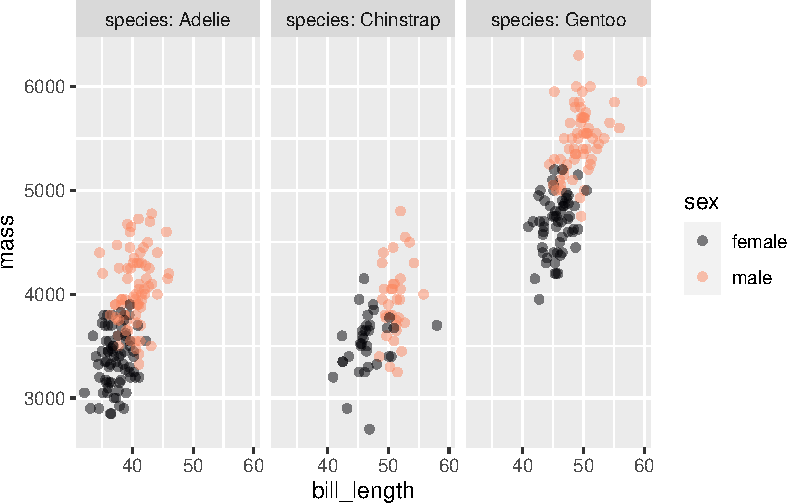
\includegraphics{test-tufte_files/figure-pdf/fig-mass-bill-species-sex2-1.pdf}

}

\caption{\label{fig-mass-bill-species-sex2}The same data as in
Figure~\ref{fig-mass-bill-species}(b), but with \texttt{sex} mapped to
color and \texttt{species} mapped to facet. This changes the visual
impression created.}

\end{figure}%

\subsection{Graphical annotations}\label{graphical-annotations}

We can enhance our interpretion of patterns in the dots of a point plot
by \emph{adding ``notes''} to the graphic, in other words,
``\textbf{annotating}'' the graphic. Lessons
\ref{sec-variation-and-distribution} and \ref{sec-model-annotation}
introduce different formats of statistical annotations that highlight
different features of the data.

Here, to illustrate what we mean by a graphical annotation, we will use
a familiar non-statistical annotation.
Figure~\ref{fig-cities-with-continents} replots the locations of world
cities with an annotation showing continents and islands.

\begin{figure}

\centering{

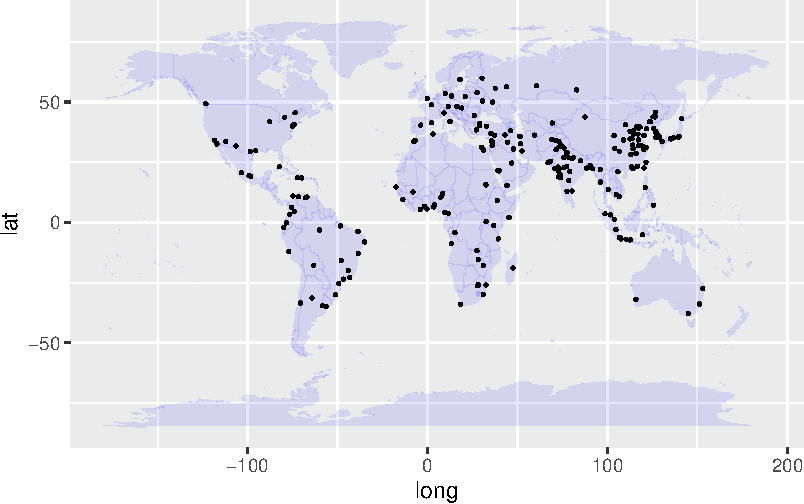
\includegraphics{test-tufte_files/figure-pdf/fig-cities-with-continents-1.pdf}

}

\caption{\label{fig-cities-with-continents}The latitude and longitude of
the world's 250 biggest cities annotated with a map of the continents
and major islands.}

\end{figure}%

Data shown without an annotation (Figure~\ref{fig-world-cities}) may
suggest a pattern. Adding an appropriate annotation enables you to judge
the existence with the intuited pattern with much more confidence or,
conversely, reject the pattern as a cloud-like illusion.

\newpage

\section{Variation and density,
graphically}\label{sec-variation-and-distribution}

\begin{quote}
\emph{Variation itself is nature's only irreducible essence. Variation
is the hard reality, not a set of imperfect measures for a central
tendency. Means and medians are the abstractions.} ----- Stephen Jay
Gould (1941- 2002), paleontologist and historian of science.
\end{quote}

The point plots introduced in Lesson \ref{sec-point_plots} are designed
to show relationships between variables. Much of statistical thinking
involves discovering, quantifying, and verifying such relationships. We
have already introduced a concept structure for talking about
relationships between variables: one variable is identified as the
\textbf{response variable} and others as the \textbf{explanatory
variables}. In point plots, we use the vertical axis for the response
variable and the horizontal axis, color, and faceting for the
explanatory variables.

Our focus in this Lesson is on describing the response variable.
Remember that the origin of the word ``variable''
{\marginnote{\begin{footnotesize}We mean ``variable'' in the statistical
sense. People also talk about variables in algebra, which is only
distantly connected with statistics.\end{footnotesize}}} is in the
specimen-to-specimen \emph{variation} in values. We will look at
variation in two distinct ways: 1) in this Lesson, the \emph{shape} of
the variation, and 2) in Lesson \ref{sec-accounting-for-variation}, the
\emph{amount} of the variation.

\subsection{The ``shape'' of variation}\label{the-shape-of-variation}

We turn to a familiar situation to illustrate variation: pregnancy and
the duration of gestation---the time from conception to birth. It's well
known that typical human gestation is about nine months. But it varies
from one birth to another. We can describe this variation using the
\texttt{Births2022} data frame, a random sample of 20,000 births from
the Centers for Disease Control's census of 3,699,040 US births in 2022.
The \texttt{duration} variable records the (estimated) period of
gestation in weeks.

Figure~\ref{fig-gestation-duration1}(a) shows just the \texttt{duration}
variable. {\marginnote{\begin{footnotesize}The tilde expression used is
\texttt{duration\ \textasciitilde{}\ 1}, where \texttt{1} signifies that
there are no explanatory variables.\end{footnotesize}}} It's easy to see
that durations longer than 45 weeks are rare. ``Extremely preterm''
births---defined as birth before the 28th week of gestation, are also
uncommon. Most common are births at about 39 weeks, that is, about 9
months. The (vertical) spread of the dots shows the extent of variation
in \texttt{duration}. The most common outcomes are at the value of
\texttt{duration} where the dots have the most ``\textbf{density}.''

\begin{Shaded}
\begin{Highlighting}[]
\NormalTok{Births2022 }\SpecialCharTok{|\textgreater{}} 
  \FunctionTok{point\_plot}\NormalTok{(duration }\SpecialCharTok{\textasciitilde{}} \DecValTok{1}\NormalTok{,}
             \CommentTok{\# arguments specifying graphic details}
             \AttributeTok{point\_ink =} \FloatTok{0.1}\NormalTok{, }\AttributeTok{size =} \FloatTok{0.2}\NormalTok{, }\AttributeTok{jitter=}\StringTok{"y"}\NormalTok{)}
\NormalTok{Births2022 }\SpecialCharTok{|\textgreater{}} 
  \FunctionTok{point\_plot}\NormalTok{(duration }\SpecialCharTok{\textasciitilde{}} \DecValTok{1}\NormalTok{, }\AttributeTok{annot=}\StringTok{"violin"}\NormalTok{,}
             \CommentTok{\# graphic details}
             \AttributeTok{point\_ink =} \FloatTok{0.1}\NormalTok{, }\AttributeTok{size =} \FloatTok{0.2}\NormalTok{, }\AttributeTok{bw=}\FloatTok{0.5}\NormalTok{, }\AttributeTok{jitter=}\StringTok{"y"}\NormalTok{) }
\end{Highlighting}
\end{Shaded}

\begin{figure}

\begin{minipage}{0.50\linewidth}

\centering{

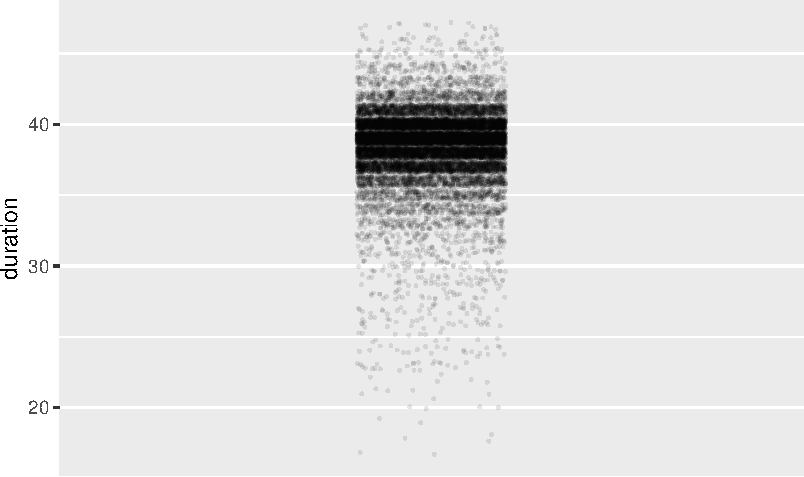
\includegraphics{test-tufte_files/figure-pdf/fig-gestation-duration1-1.pdf}

}

\subcaption{\label{fig-gestation-duration1-1}Just the (jittered) data.}

\end{minipage}%
%
\begin{minipage}{0.50\linewidth}

\centering{

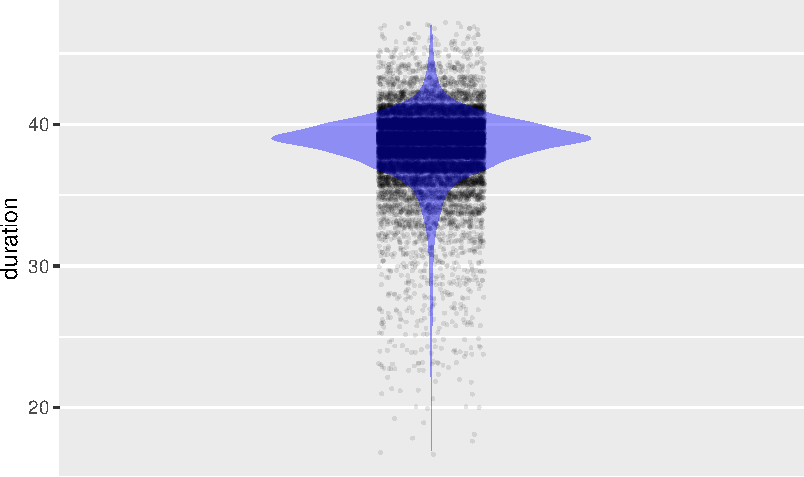
\includegraphics{test-tufte_files/figure-pdf/fig-gestation-duration1-2.pdf}

}

\subcaption{\label{fig-gestation-duration1-2}Annotating with a violin
plot.}

\end{minipage}%

\caption{\label{fig-gestation-duration1}The \texttt{duration} (in weeks)
of gestation for each of 20,000 randomly selected 2022 births in the US}

\end{figure}%

For many people, the dots drawn in a point plot are reminiscent of seeds
or pebbles scattered across an area.
{\marginnote{\begin{footnotesize}Indeed, a popular synonym for ``point
plot'' is ``scatter-plot.''\end{footnotesize}}} Density can be high in
some areas, lower in others, negligible or nil in others. The spatial
density pattern is called the ``\textbf{distribution}'' of the variable.

Many people can perceive density in a point plot without any need to
count or calculate; it is an intuitive mode of perception. To
illustrate, Figure~\ref{fig-density-explain} is a made-up point plot
with five patches of different densities. The densities are 25, 50, 100,
200, and 400 points per unit area. Many people find it easy and
immediate to point out the most dense patches and even to put the
patches in order by density. However, people are hard put to qualify
even the \emph{relative} densities. For instance, the largest patch has
a smaller density than the next largest patch, but quantifying this by
eye (without being told the densities) is not really possible.

\begin{marginfigure}

\centering{

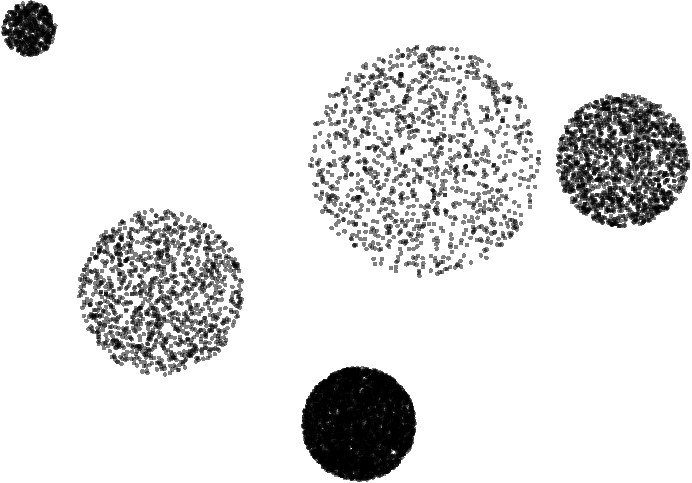
\includegraphics{test-tufte_files/figure-pdf/fig-density-explain-1.pdf}

}

\caption{\label{fig-density-explain}Five point-plot patches of different
sizes and densities. The density can be perceived independently of the
area.}

\end{marginfigure}%

Our eye gives a qualitative estimate of relative density, not a precise
quantitative one. Our graphical perception is more precise when it comes
to length or width. Ingeniously, designers of statistical graphics have
created an annotation---called a ``\textbf{violin}''---that shows the
density in terms of width. Figure~\ref{fig-gestation-duration1}(b) adds
a violin annotation to the point plot.

\begin{tcolorbox}[enhanced jigsaw, colbacktitle=quarto-callout-note-color!10!white, opacityback=0, breakable, opacitybacktitle=0.6, colback=white, coltitle=black, arc=.35mm, title=\textcolor{quarto-callout-note-color}{\faInfo}\hspace{0.5em}{Example: Do twins take longer?}, left=2mm, colframe=quarto-callout-note-color-frame, rightrule=.15mm, bottomrule=.15mm, leftrule=.75mm, bottomtitle=1mm, toptitle=1mm, titlerule=0mm, toprule=.15mm]

Violins can be informative when comparing two or more levels of an
explanatory variable. To illustrate, consider the duration of gestation
for twins versus singletons. Let's see if the distribution of durations
is different for the different kinds of birth.

\begin{Shaded}
\begin{Highlighting}[]
\NormalTok{Births2022 }\SpecialCharTok{|\textgreater{}} 
  \FunctionTok{filter}\NormalTok{(plurality }\SpecialCharTok{\textless{}} \DecValTok{3}\NormalTok{) }\SpecialCharTok{|\textgreater{}}
  \FunctionTok{mutate}\NormalTok{(}\AttributeTok{plurality =} \FunctionTok{factor}\NormalTok{(plurality, }\AttributeTok{labels =} \FunctionTok{c}\NormalTok{(}\StringTok{"singleton"}\NormalTok{, }\StringTok{"twin"}\NormalTok{))) }\SpecialCharTok{|\textgreater{}}
  \FunctionTok{point\_plot}\NormalTok{(duration }\SpecialCharTok{\textasciitilde{}}\NormalTok{ plurality,  }\AttributeTok{annot=}\StringTok{"violin"}\NormalTok{,}
            \CommentTok{\# the following specify graphics details }
            \AttributeTok{point\_ink =} \FloatTok{0.1}\NormalTok{, }\AttributeTok{size =} \FloatTok{0.2}\NormalTok{, }\AttributeTok{bw=}\FloatTok{0.5}\NormalTok{, }
            \AttributeTok{jitter=}\StringTok{"y"}\NormalTok{, }\AttributeTok{model\_ink=}\FloatTok{0.5}\NormalTok{) }
\end{Highlighting}
\end{Shaded}

\begin{figure}[H]

\sidecaption{\label{fig-duration-plurality}The distribution of
\texttt{duration} shown separately for singletons, twins, and (a handful
of) triplets.}

\centering{

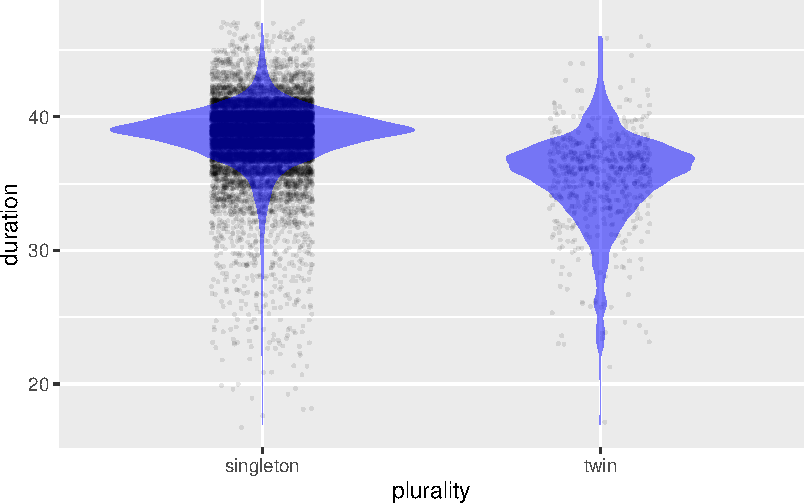
\includegraphics{test-tufte_files/figure-pdf/fig-duration-plurality-1.pdf}

}

\end{figure}%

In Figure~\ref{fig-duration-plurality}, the density of points is vastly
different for different levels of plurality. The jitter-column of
singletons is much denser than for twins. Singletons are much more
common than twins.

Even though there are many more singletons than twins, the violins are
roughly the same width. This is by design. The violins in
Figure~\ref{fig-duration-plurality} tell the story of birth-to-birth
variation of duration \emph{within} each group. For twins, durations
near 36 weeks are much more common than durations near 39 weeks.
Similarly, comparing the two violins shows that premature births are
much more likely for twins than for singletons. We can see this from the
violins despite the fact that the large majority of premature births are
of singletons.

It's worth emphasizing the previous point since it will be fundamental
to statistical thinking.

\end{tcolorbox}

\subsection{Some simple shapes}\label{some-simple-shapes}

There are infinitely many different shapes of distributions. Even so, a
few simple shapes are common. These are shown in panels (a)-(d) of
Figure~\ref{fig-violin-shapes}. Panel (e) is a more complicated shape,
infrequently seen in practice. (Unless you are practicing music rather
than statistics!)

\begin{figure}

\begin{minipage}{0.20\linewidth}

\centering{

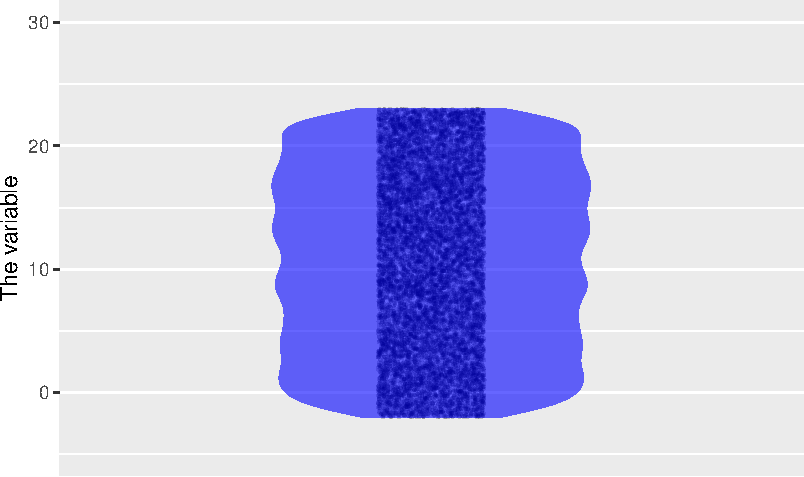
\includegraphics{test-tufte_files/figure-pdf/fig-violin-shapes-1.pdf}

}

\subcaption{\label{fig-violin-shapes-1}Uniform}

\end{minipage}%
%
\begin{minipage}{0.20\linewidth}

\centering{

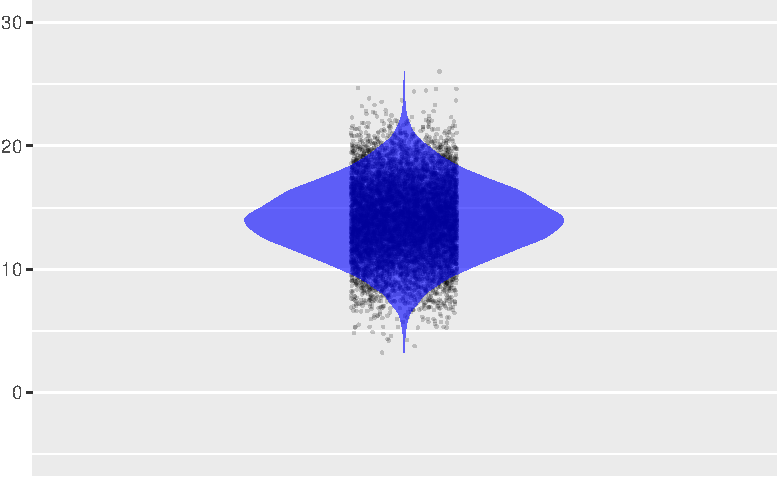
\includegraphics{test-tufte_files/figure-pdf/fig-violin-shapes-2.pdf}

}

\subcaption{\label{fig-violin-shapes-2}Normal}

\end{minipage}%
%
\begin{minipage}{0.20\linewidth}

\centering{

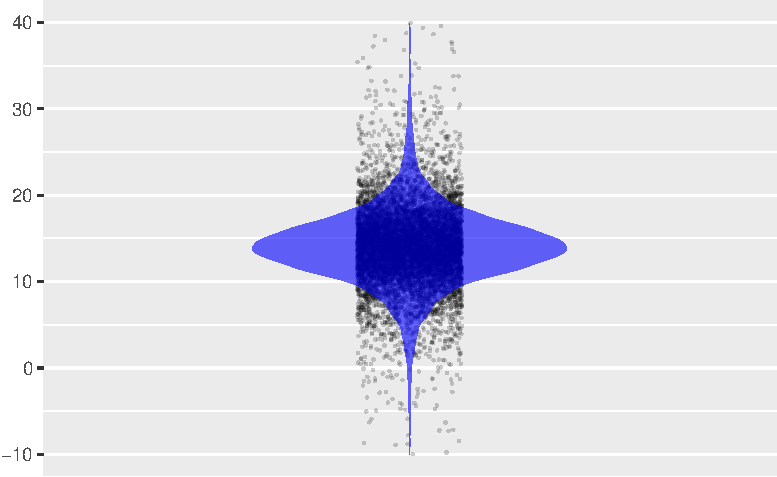
\includegraphics{test-tufte_files/figure-pdf/fig-violin-shapes-3.pdf}

}

\subcaption{\label{fig-violin-shapes-3}Long tailed}

\end{minipage}%
%
\begin{minipage}{0.20\linewidth}

\centering{

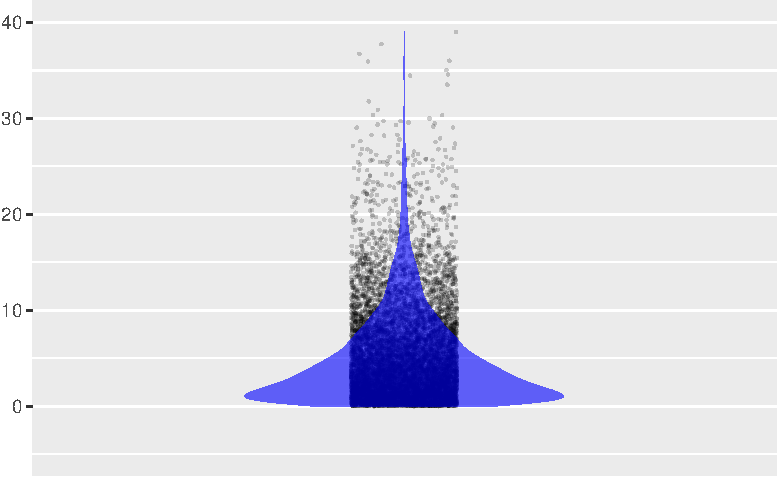
\includegraphics{test-tufte_files/figure-pdf/fig-violin-shapes-4.pdf}

}

\subcaption{\label{fig-violin-shapes-4}Skew}

\end{minipage}%
%
\begin{minipage}{0.20\linewidth}

\centering{

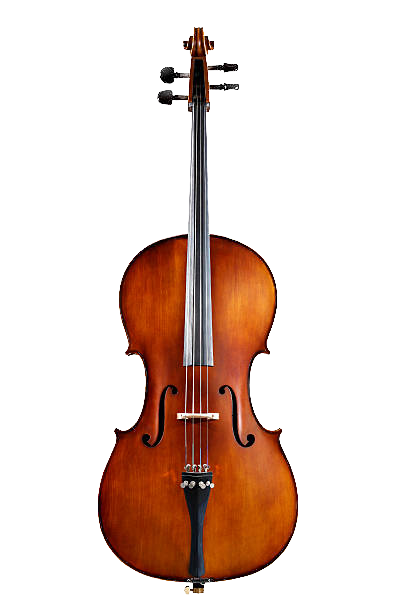
\includegraphics[width=1.37in,height=\textheight]{www/real-violin.png}

}

\subcaption{\label{fig-violin-shapes-5}A cello!}

\end{minipage}%

\caption{\label{fig-violin-shapes}Various distribution shapes}

\end{figure}%

Figure~\ref{fig-violin-shapes}(a) is a ``\textbf{uniform}''
distribution, where each possible value is more or less equally likely.
It's not so common to see this in real-world data. When you do, it's a
good sign that something artificial or mathematical is behind the
data-generating process.

Much more common is the so-called ``\textbf{normal}'' distribution of
Figure~\ref{fig-violin-shapes}(b). The name given to it, ``normal,'' is
an indication of how commonly it is seen. There is a region of highest
density at middle values, with the density falling off symmetrically
toward higher and lower values in a ``bell-shaped'' fashion.

Other common patterns in distribution have a single peak (like the
normal distribution) but have ``tails'' that extend much further than in
the normal distribution. These are sometimes called
``\textbf{long-tailed} distributions. In
Figure~\ref{fig-violin-shapes}(c), the long tails are symmetrical around
the peak, while in Figure~\ref{fig-violin-shapes}(d), there is only one
long tail. Such one-sided, long-tailed distributions are
called''\textbf{skew}'' distributions. Skew distributions are
particularly common in economic data such as personal or national
income.

There have been society-wide consequences to ignoring skewness in favor
of ``well-behaved,'' short-tailed distributions such as the so-called
normal distribution. For instance, the 2008 ``Great Recession'' was
partly due to mistakenly high values on mortgage-backed and other
financial securities. Financial analysts used valuation techniques that
would be appropriate for normal distributions of risky events, but were
utterly inadequate in the face of skew distributions.

\begin{tcolorbox}[enhanced jigsaw, colbacktitle=quarto-callout-note-color!10!white, opacityback=0, breakable, opacitybacktitle=0.6, colback=white, coltitle=black, arc=.35mm, title=\textcolor{quarto-callout-note-color}{\faInfo}\hspace{0.5em}{Example: Skew storms}, left=2mm, colframe=quarto-callout-note-color-frame, rightrule=.15mm, bottomrule=.15mm, leftrule=.75mm, bottomtitle=1mm, toptitle=1mm, titlerule=0mm, toprule=.15mm]

A life-threatening setting for skew distributions concerns extreme
events like large storms and fires.

\begin{Shaded}
\begin{Highlighting}[]
\NormalTok{Monocacy\_river }\SpecialCharTok{|\textgreater{}} 
  \FunctionTok{point\_plot}\NormalTok{(precip }\SpecialCharTok{\textasciitilde{}} \DecValTok{1}\NormalTok{, }\AttributeTok{annot=}\StringTok{"violin"}\NormalTok{)}
\NormalTok{US\_wildfires }\SpecialCharTok{|\textgreater{}} 
  \FunctionTok{point\_plot}\NormalTok{(area }\SpecialCharTok{\textasciitilde{}} \DecValTok{1}\NormalTok{, }\AttributeTok{annot=}\StringTok{"violin"}\NormalTok{)}
\end{Highlighting}
\end{Shaded}

\begin{figure}[H]

\begin{minipage}{0.50\linewidth}

\centering{

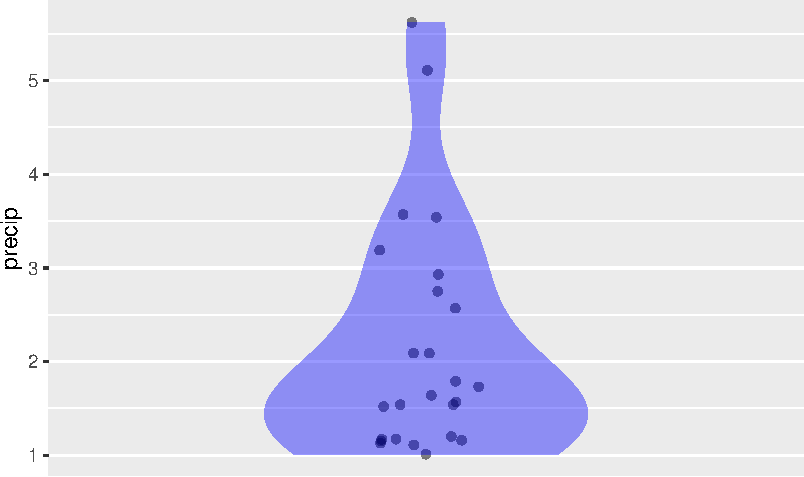
\includegraphics{test-tufte_files/figure-pdf/fig-extreme-storm-fires-1.pdf}

}

\subcaption{\label{fig-extreme-storm-fires-1}Inches of rain in storms in
Maryland}

\end{minipage}%
%
\begin{minipage}{0.50\linewidth}

\centering{

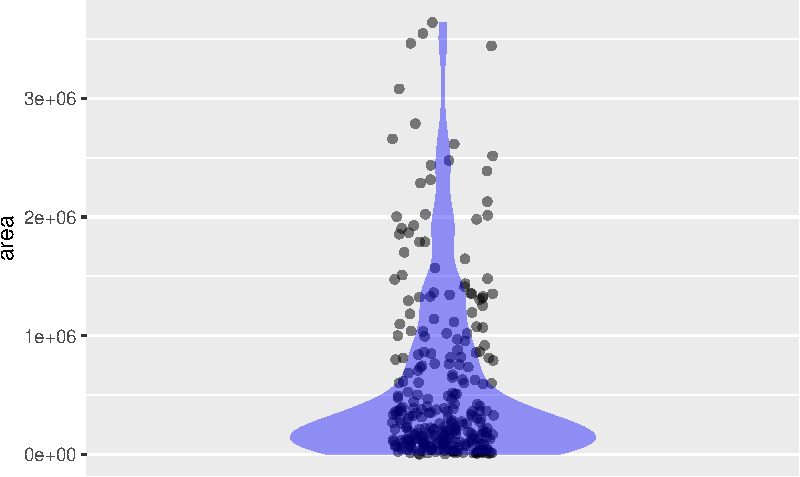
\includegraphics{test-tufte_files/figure-pdf/fig-extreme-storm-fires-2.pdf}

}

\subcaption{\label{fig-extreme-storm-fires-2}Area burned by wildfires in
the US each month}

\end{minipage}%

\caption{\label{fig-extreme-storm-fires}Examples of skew distributions}

\end{figure}%

\end{tcolorbox}

In this Lesson, we have emphasized the ``shape'' of variation, that is,
the pattern of which values are more common and which less common. In
Lesson \ref{sec-variation} we turn to another aspect of variation that
is central to statistical thinking: the \textbf{amount of variation}.
Variation can be measured numerically, just as distance or position can
be measured numerically. Happily, as we will see in Lesson
\ref{sec-variation}, the name of the quantity often used to measure
variation has a name---``\textbf{variance}''---that reflects exactly
what it measures: variation.

\newpage

\section{Annotating point plots with a
model}\label{sec-model-annotation}

Lesson Chapter~\ref{sec-variation-and-distribution} introduced the
violin-plot annotation to display graphically the ``shape'' of
variation: which values are more common, which values rare, and which
values never seen at all. In this Lesson, we turn to a completely
different sort of annotation showing a ``\textbf{statistical model}.''
Models provide a way to summarize quantitatively the
\textbf{relationships} among variables.

\subsection{Simple models}\label{simple-models}

We define a ``\textbf{simple model}'' as a model with a single
explanatory variable. We will be using simple models frequently, but
also models with more than one explanatory variable. (\emph{All} the
models we consider in these Lessons have a single \emph{response}
variable.) To illustrate, let's return to the anthropometric
measurements displayed in Figure~\ref{fig-wrist-ankle} where the
explanatory variable is ankle circumference. Adding a statistical model
annotation is accomplished by using the argument
\texttt{annot\ =\ "model"}:

\begin{Shaded}
\begin{Highlighting}[]
\NormalTok{Anthro\_F }\SpecialCharTok{|\textgreater{}} \FunctionTok{point\_plot}\NormalTok{(Wrist }\SpecialCharTok{\textasciitilde{}}\NormalTok{ Ankle, }\AttributeTok{annot =} \StringTok{"model"}\NormalTok{)}
\end{Highlighting}
\end{Shaded}

\begin{figure}[H]

\sidecaption{\label{fig-wrist-ankle-annot}Annotating
\texttt{Wrist\ \textasciitilde{}\ Ankle} point plot with a statistical
model.}

\centering{

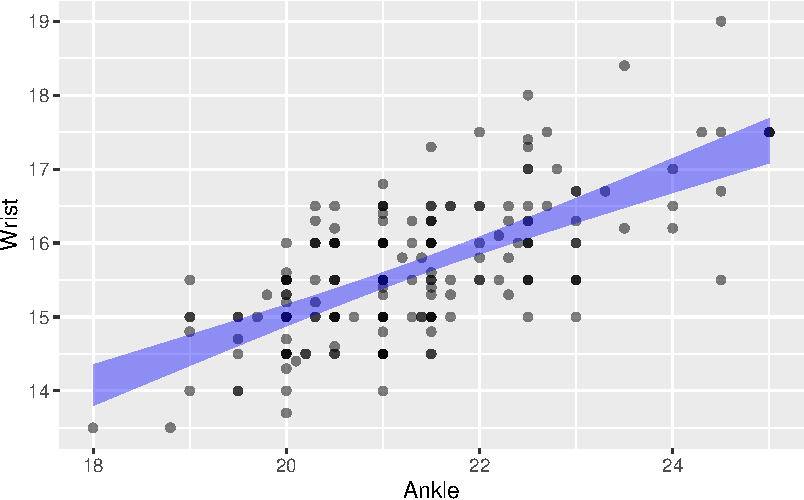
\includegraphics{test-tufte_files/figure-pdf/fig-wrist-ankle-annot-1.pdf}

}

\end{figure}%

The model annotation is drawn as a more-or-less straight band, shaded
blue, to help distinguish it from individual data points. By default,
\texttt{point\_plot()} looks for a ``\textbf{linear}'' pattern in the
data; the band is straight because we asked for it to be straight. The
particular band presented by \texttt{point\_plot()} is the one that
comes as close as possible to the data points. ``As close as possible''
is defined in a specific way which we'll investigate later; for now it
suffices to note that the band goes nicely through the cloud of data
points.

The explanatory variable in Figure~\ref{fig-wrist-ankle-annot} is
\emph{quantitative}. Model annotations can also be drawn for
\emph{categorical} explanatory variables. To illustrate, consider the
data in \texttt{Birdkeepers}, used in a study of smoking, bird-keeping,
and lung cancer. The unit of observation is an individual person. The
variable \texttt{YR} records the number of years that person smoked,
while the categorical variable \texttt{LC} indicates whether the person
had been diagnosed with lung cancer. The data and a model annotation are
shown in Figure~\ref{fig-birdkeepers-A}

\begin{Shaded}
\begin{Highlighting}[]
\NormalTok{Birdkeepers }\SpecialCharTok{|\textgreater{}} \FunctionTok{point\_plot}\NormalTok{(YR }\SpecialCharTok{\textasciitilde{}}\NormalTok{ LC, }\AttributeTok{annot=}\StringTok{"model"}\NormalTok{)}
\end{Highlighting}
\end{Shaded}

\begin{figure}

\sidecaption{\label{fig-birdkeepers-A}Years of cigarette smoking versus
diagnostic status for lung cancer.}

\centering{

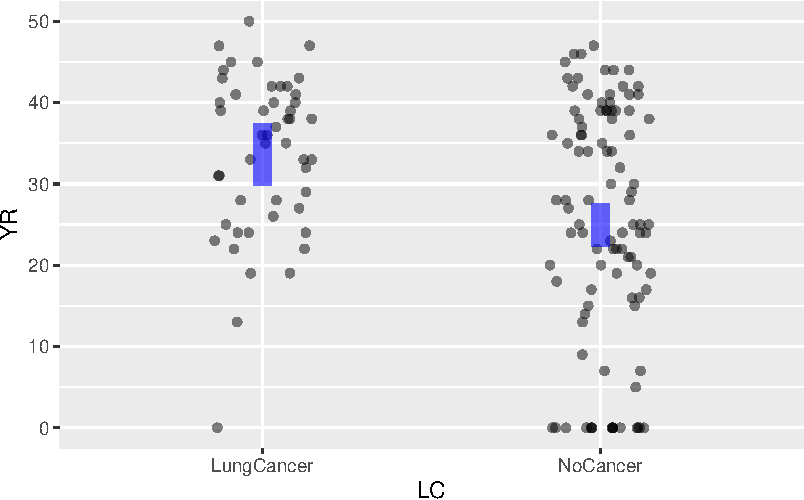
\includegraphics{test-tufte_files/figure-pdf/fig-birdkeepers-A-1.pdf}

}

\end{figure}%

For a categorical explanatory variable, the model annotation is a
vertical band (or ``\textbf{interval}'') for each of the categorical
levels. As with the band Figure~\ref{fig-wrist-ankle-annot}, the model
annotation in Figure~\ref{fig-birdkeepers-A} is vertically centered
among the data points.

In later Lessons, we will discuss how \texttt{point\_plot()} chooses the
specific model annotation shown in any given case. But consider these
closely related questions:

\begin{itemize}
\tightlist
\item
  Why are the model annotations shown as a band or interval, rather than
  as a single, simple line or single numerical value for each category?
\item
  What do the model annotations tell us?
\end{itemize}

The bands or intervals in the model annotations shown by
\texttt{point\_plot()} are there as a reminder that the data are
consistent with a range of models. The height of the band/interval shows
how large is that range. This is essential to drawing conclusions from
the plots. For instance, in Figure~\ref{fig-birdkeepers-A}, the
intervals for two levels ``lung cancer'' and ``no cancer'' have no
vertical overlap. This tells the statistical thinker to be confident in
a claim that the typical value of \texttt{YR} is genuinely different
between the two levels. If the intervals had overlapped vertically, the
statistical thinker would know to be skeptical about such a claim.

Similarly, in Figure~\ref{fig-wrist-ankle-annot} the model annotation is
a sloping band. The slope indicates that \texttt{Ankle} and
\texttt{Wrist} are related to one another: larger \texttt{Wrists} tend
to go along with larger \texttt{Ankles}. If the two variables were
unrelated, we would expect the band to run horizontally---zero
slope---meaning that the typical wrist circumference is the same for all
people, regardless of the ankle circumference. The vertical thickness of
the band tells the statistical thinker a range of plausible slopes that
match the data. In Figure~\ref{fig-wrist-ankle}, there is no horizontal
line that can be drawn from end to end \emph{within} the band. Thus, the
statistical thinker can be confident that there is a non-zero slope
describing the relationship between \texttt{Wrist} and \texttt{Ankle}.

You may have encountered statistical graphics similar to those in
\textbf{?@fig-point-estimate} but with an essential difference, the
model annotations are lines rather than bands or intervals. In
\textbf{?@fig-point-estimate}, the model annotations are simple lines
that in principle are infinitely thin. With a numerical explanatory
variable, the model annotation is a line that can have a non-zero slope.
In contrast, for a categorical explanatory variable, there is a
horizontal line drawn at a single vertical value for each level of the
explanatory variable. Such simplified graphics do not recognize that, in
reality, there is a range of different lines that are plausible models.
Since we can't tell from graphics like \textbf{?@fig-point-estimate}
what is the range of plausible models, the annotation provides no
guidance about whether to be confident that the data tell us slopes or
vertical differences are non-zero.

Statistical thinking makes extensive use of the concept that there is a
range of plausible models consistent with the data. Any straight line
that falls into the band in Figure~\ref{fig-wrist-ankle} is a plausible
model of the data. In Figure~\ref{fig-birdkeepers-A}, any pair of values
that fall into vertical intervals are a plausible model of the data.

\begin{figure}

\centering{

\begin{figure}[H]

\begin{minipage}{0.50\linewidth}

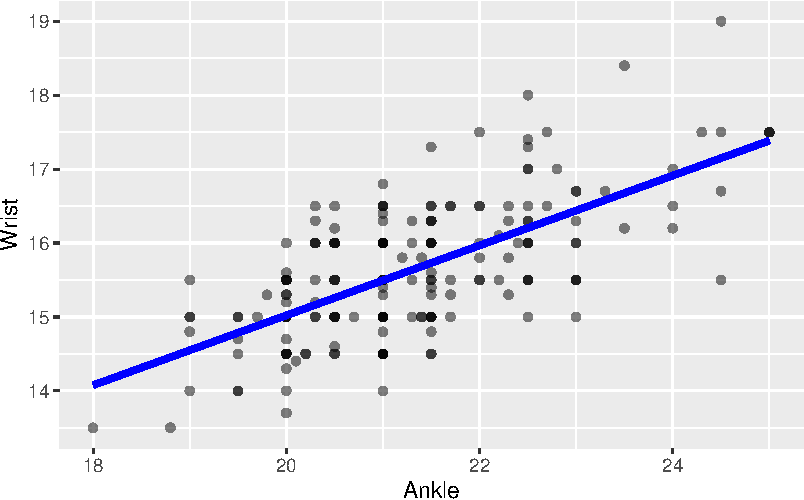
\includegraphics{test-tufte_files/figure-pdf/unnamed-chunk-62-1.pdf}

\subcaption{\label{}Straight-line}
\end{minipage}%
%
\begin{minipage}{0.50\linewidth}

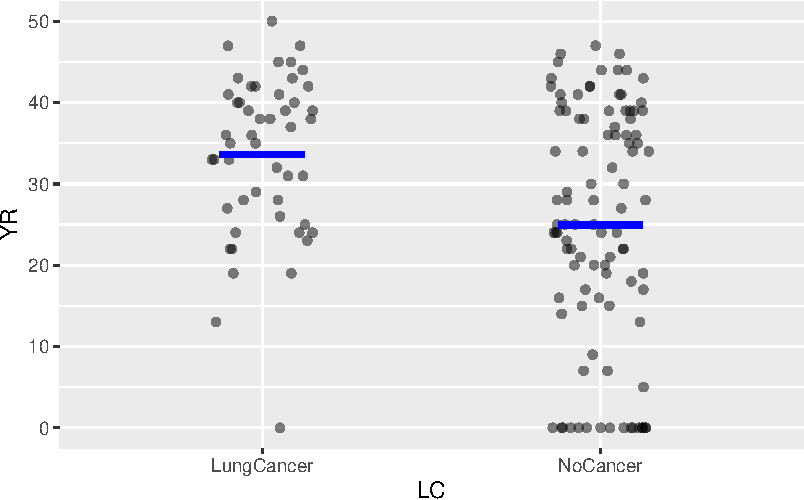
\includegraphics{test-tufte_files/figure-pdf/unnamed-chunk-62-2.pdf}

\subcaption{\label{}Discrete values}
\end{minipage}%

\end{figure}%

}

\caption{\label{fig-point-estimate.column-page-right}Many statistical
texts present models as a straight line or as discrete values. This
omits essential information compared to the model annotations generated
by \texttt{point\_plot()}.}

\end{figure}%

\begin{tcolorbox}[enhanced jigsaw, colbacktitle=quarto-callout-note-color!10!white, opacityback=0, breakable, opacitybacktitle=0.6, colback=white, coltitle=black, arc=.35mm, title=\textcolor{quarto-callout-note-color}{\faInfo}\hspace{0.5em}{``Trend'' or ``cause''}, left=2mm, colframe=quarto-callout-note-color-frame, rightrule=.15mm, bottomrule=.15mm, leftrule=.75mm, bottomtitle=1mm, toptitle=1mm, titlerule=0mm, toprule=.15mm]

Each of the plausible models---as in Figures \ref{fig-wrist-ankle-annot}
or \ref{fig-birdkeepers-A}---describes a specific relationship between
the response and explanatory variables. For the wrist/ankle
relationship, the plausible models all show a ``trend'' between ankle
size and wrist size. For the smoking-years/lung-cancer relationship, the
people with lung cancers ``tend'' to have smoken for more years than the
no-cancer people.

The words ``trend'' or ``tend'' are weak. Often, statistical thinkers
are interested in stronger statements, like these:

\begin{itemize}
\tightlist
\item
  Larger ankles \emph{cause} larger wrists.
\item
  Smoking for more years \emph{increases the chances} of lung cancer.
\end{itemize}

We can call these \textbf{opinionated statements} because they make use
of some hypothesis about how the world works held by the modeler rather
than being forced solely by the data. Many people think it silly to
claim that ``larger ankles \emph{cause} larger wrists.'' It seems much
more probable that ``larger people have larger wrists and also larger
ankles.'' On the other hand, many people will be sympathetic to the
statement ``increases the chances of lung cancer.'' They have heard such
things from other respected sources.

Some of the techniques covered in these \emph{Lessons} are designed to
substantiate or undermine opinionated statements like these. Until we
understand and use these techniques, it is dicey to quantitatively
support an opinionated statement from data.

Many statisticians prefer to avoid the whole matter of opinionated
statements. {\marginnote{\begin{footnotesize}But see Lesson
\ref{sec-experiment} for an approach approved by even the most
opinion-wary statistician.\end{footnotesize}}} Weak, unopinionated
language like ``trend'' or ``tend'' are used instead. Those preferring
more technical-sounding language might use ``associated with'' or
``correlated with.''

\end{tcolorbox}

\subsection{Independence}\label{independence}

We use model annotations to display whether variables are related. It's
good to consider as well a particular type of relationship:
independence. When the explanatory variable is categorical, the model
annotations will be a vertical interval for each level. When the
response is independent of the explanatory variable, those intervals
will overlap. For instance, in \textbf{?@fig-independence}(a) values of
\texttt{YR} near 30 are in both vertical intervals.

For a quantitative explanatory variable, as in
\textbf{?@fig-independence}(b), independent variables will have a model
band that is more-or-less horizontal. That is to say, at least one
horizontal line will fall within the band.

\begin{figure}

\centering{

\begin{figure}[H]

\begin{minipage}{0.50\linewidth}

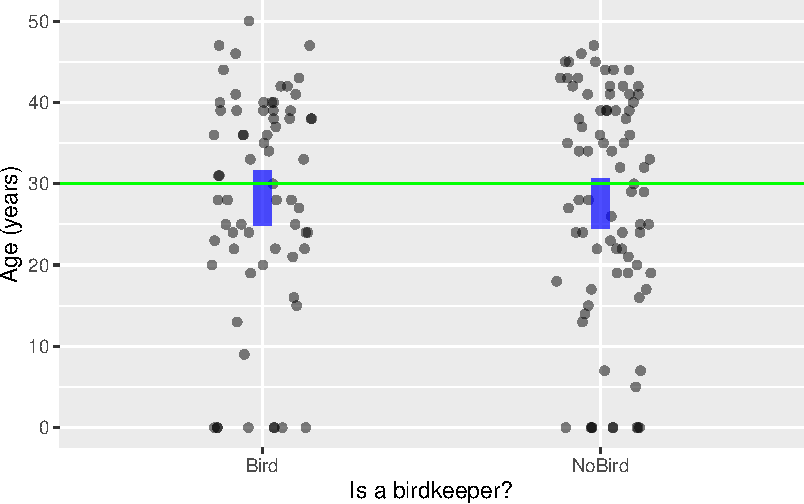
\includegraphics{test-tufte_files/figure-pdf/unnamed-chunk-63-1.pdf}

\subcaption{\label{}Categorical explanatory variable}
\end{minipage}%
%
\begin{minipage}{0.50\linewidth}

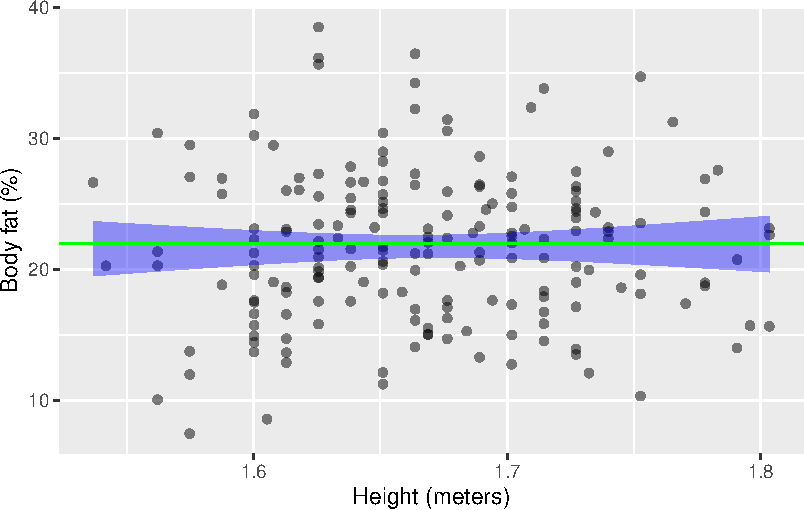
\includegraphics{test-tufte_files/figure-pdf/unnamed-chunk-63-2.pdf}

\subcaption{\label{}Quantitative explanatory variable}
\end{minipage}%

\end{figure}%

}

\caption{\label{fig-independence.column-page-right}Model annotations
consistent with the response and explanatory variables being
independent. Panel (a) considers whether the age of the people in
\texttt{Birdkeepers} is independent of whether the person keeps a bird.
Panel (b), based on \texttt{Anthro\_F} is about the possible
relationship between a person's height and body fat as a percent of
overall mass}

\end{figure}%

\subsection{Multiple explanatory
variables}\label{multiple-explanatory-variables}

In Lesson \ref{sec-point_plots} we used color and faceting to look at
the response variable in terms of up to three explanatory variables.
Statistical models can also handle multiple explanatory variables.

We'll illustrate with a commentary from a political pundit about
education spending in US schools:

\begin{quote}
\emph{{[}T{]}he 10 states with the lowest per pupil spending included
four --- North Dakota, South Dakota, Tennessee, Utah --- among the 10
states with the top SAT scores. Only one of the 10 states with the
highest per pupil expenditures --- Wisconsin --- was among the 10 states
with the highest SAT scores. New Jersey has the highest per pupil
expenditures, an astonishing \$10,561, which teachers' unions elsewhere
try to use as a negotiating benchmark. New Jersey's rank regarding SAT
scores? Thirty-ninth\ldots{} The fact that the quality of
schools\ldots{} {[}fails to correlate{]} with education appropriations
will have no effect on the teacher unions' insistence that money is the
crucial variable.}-----George F. Will, (September 12, 1993),
``Meaningless Money Factor,'' The Washington Post, C7.
\end{quote}

The opinionated claim here is that ``money is the crucial variable'' in
educational outcomes. George Will seeks to rebut this claim with data.
Fortunately for us, actual data on SAT scores and per pupil expenditures
in the mid-1990s is available in the \texttt{mosaicData::SAT} data
frame. The unit of observation in \texttt{SAT} is a US state.
Figure~\ref{fig-SAT-one}(a) shows an annotated point plot of
state-by-state expenditures and test scores. The trend signaled by the
model annotation is that SAT scores are slightly lower in
high-expenditure states, consistent will George Will's observations. But
\ldots{}

\begin{figure*}

\centering{

\begin{figure}[H]

\begin{minipage}{0.50\linewidth}

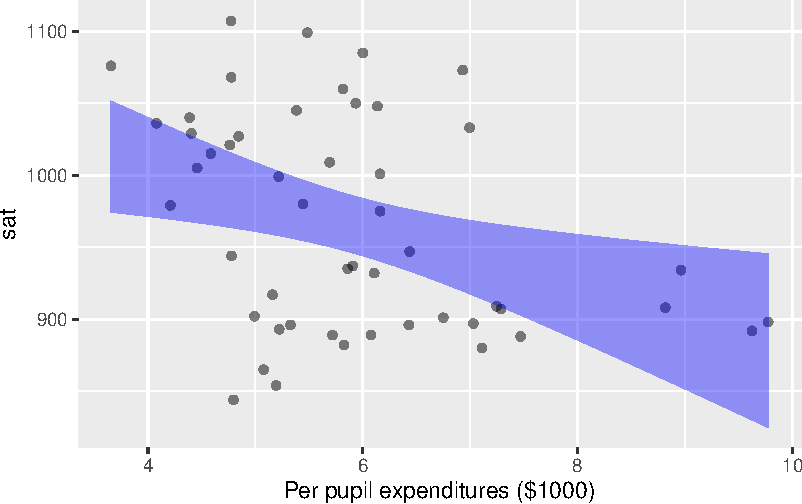
\includegraphics{test-tufte_files/figure-pdf/unnamed-chunk-64-1.pdf}

\subcaption{\label{}expenditures as the explanatory variable}
\end{minipage}%
%
\begin{minipage}{0.50\linewidth}

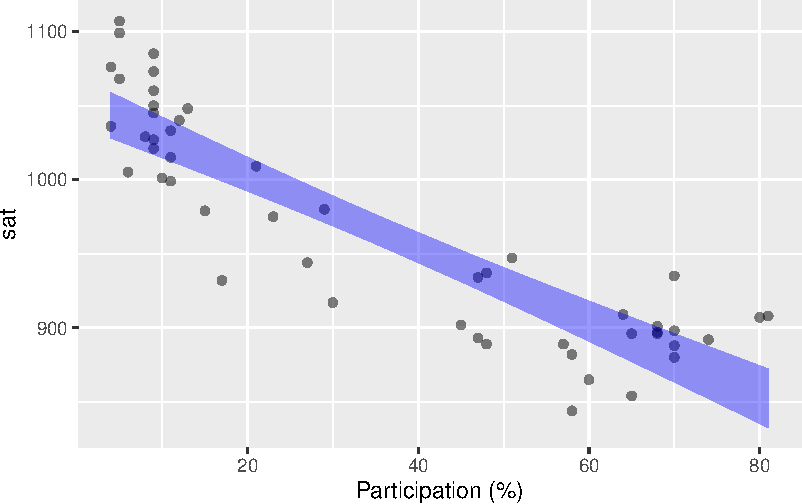
\includegraphics{test-tufte_files/figure-pdf/unnamed-chunk-64-2.pdf}

\subcaption{\label{}fraction of students taking SAT as the explanatory
variable}
\end{minipage}%

\end{figure}%

}

\caption{\label{fig-SAT-one}SAT scores as a function of per-pupil
expenditures and of fraction taking the SAT.}

\end{figure*}%

Education is a complicated matter and there are factors other than
expenditures that may be playing a role. One of these, shown in
Figure~\ref{fig-SAT-one}(b), is that participation in the SAT varies
substantially from state to state. In some states, almost all students
take the test. In others, fewer than 10\% of students take the test. The
data show a relationship between participation and scores: scores are
consistently higher in low-participation states.

\begin{Shaded}
\begin{Highlighting}[]
\NormalTok{SAT }\SpecialCharTok{|\textgreater{}} \FunctionTok{point\_plot}\NormalTok{(expend }\SpecialCharTok{\textasciitilde{}}\NormalTok{ frac, }\AttributeTok{annot=}\StringTok{"model"}\NormalTok{) }\SpecialCharTok{|\textgreater{}} 
  \FunctionTok{add\_plot\_labels}\NormalTok{(}\AttributeTok{x =}\StringTok{"Participation (\%)"}\NormalTok{, }\AttributeTok{y =} \StringTok{"Per pupil expenditures ($1000s)"}\NormalTok{)}
\end{Highlighting}
\end{Shaded}

\begin{marginfigure}

\centering{

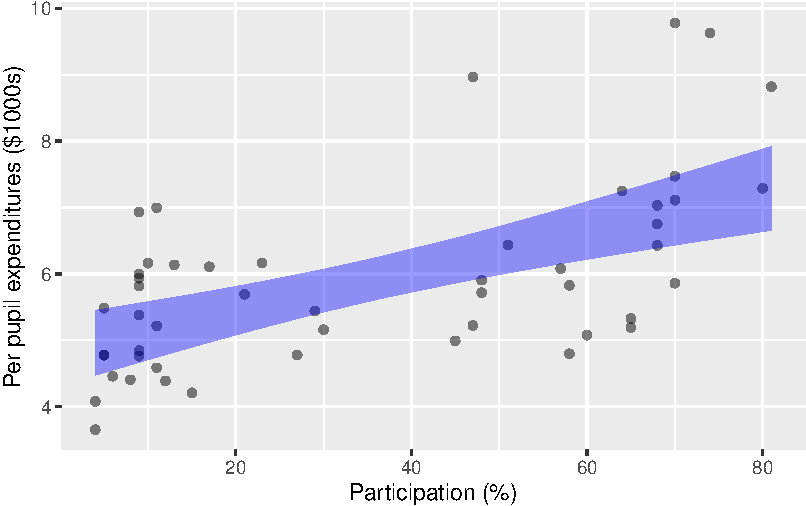
\includegraphics{test-tufte_files/figure-pdf/fig-expend-partic-1.pdf}

}

\caption{\label{fig-expend-partic}The two explanatory variables shown in
Figure~\ref{fig-SAT-one} are themselves related to one another.}

\end{marginfigure}%

Statistical modeling techniques enable us to use \emph{both}
expenditures and participation as explanatory variables.
Figure~\ref{fig-SAT-one} does this with \emph{one variable at a time}.
But we can also use both explanatory variables \emph{simultaneously}.
Doing so is important especially when there is a relationship between
the explanatory variables, as seen in the graph of expenditures versus
participation (Figure~\ref{fig-expend-partic}).

\begin{figure*}

\centering{

\begin{figure}[H]

\begin{minipage}{0.50\linewidth}

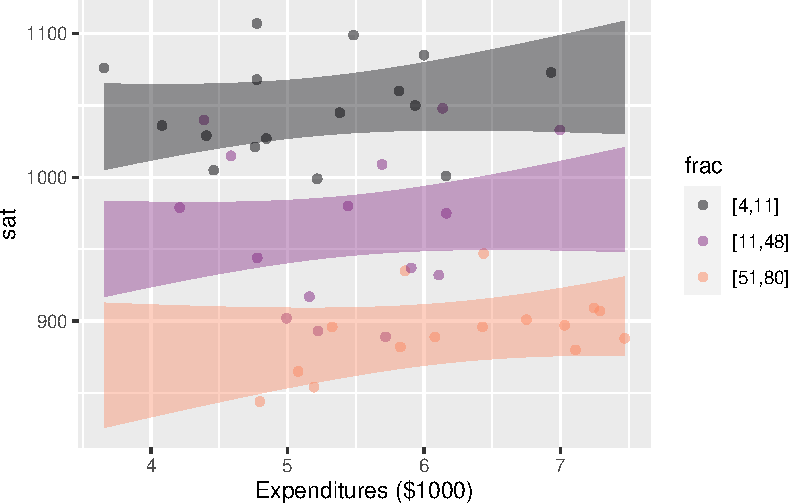
\includegraphics{test-tufte_files/figure-pdf/unnamed-chunk-66-1.pdf}

\subcaption{\label{}Expenditures on the horizontal axis, participation
as color.}
\end{minipage}%
%
\begin{minipage}{0.50\linewidth}

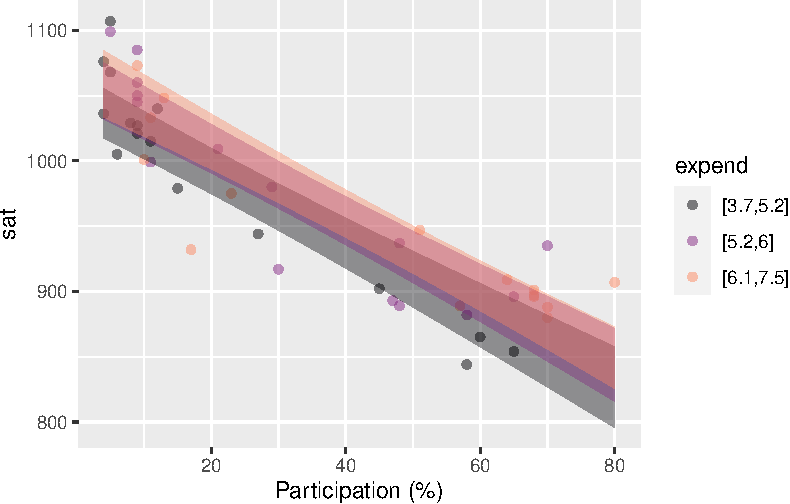
\includegraphics{test-tufte_files/figure-pdf/unnamed-chunk-66-2.pdf}

\subcaption{\label{}Expenditures as color, participation on the
horizontal axis.}
\end{minipage}%

\end{figure}%

}

\caption{\label{fig-SAT-expend-partic}A model of SAT scores as a
function of both expenditures and participation. The model is the same
for both (a) and (b), but the horizontal axis and color is reversed from
one to the other.}

\end{figure*}%

The two panels in Figure~\ref{fig-SAT-expend-partic} tell a consistent
story, but with different graphical appearances. For instance, the clear
vertical spacing between bands in the left panel indicate that SAT
scores are influenced by the participation level, even taking into
account expenditures. This appears as the downward slope in the bands in
the right panel.

But when we look at expenditures---taking into account
participation---we see horizontal bands in the left panel. (More
precisely, bands that can encompass a horizontal line.) This indicates
that we cannot confidently claim that expenditures are associated with
SAT scores. In the right panel, the lack of association between
expenditures and SAT scores is signaled by the vertical overlap between
the bands.

Many people are discomfitted to hear that looking at the same data in
different ways can lead to different conclusions. At this stage in the
\emph{Lessons} that may be true for you as well. Even so, should should
already have a concrete sense of how we can denote the ``different ways
of looking at data.'' In modeling notation, the perspective
\texttt{sat\ \textasciitilde{}\ expenditures} shows one pattern, while
the perspective
\texttt{sat\ \textasciitilde{}\ expenditures\ +\ participation} tells
another. In Lesson \ref{sec-effect-size} we will see a non-graphical way
of looking at models that makes it easier to see the effect of one
explanatory variable in the context of others. And in Lessons
\ref{sec-DAGs} and \ref{sec-experiment} we will study the methods used
in modern statistics to decide which of two possible models---say
\texttt{sat\ \textasciitilde{}\ expenditures} or
\texttt{sat\ \textasciitilde{}\ expenditures\ +\ participation}---is
more appropriate to answer questions of causation.

\newpage

\section{Data wrangling}\label{sec-wrangling}

Data wrangling refers to the organization and construction of simple
summaries of data, or preparing data in the more nuanced summaries of
statistical models. Traditionally, organizing data has been a
complicated task involving extensive computer programming. The style of
data wrangling is more modern and much less demanding for the human
wrangler. Wrangling takes advantage of the realization made only in the
last half century or so that a \emph{small set of simple operations} can
handle a large variety of re-organization tasks. The data scientist is
to learn what are these operations and how to invoke them on the
computer.

\subsection{Basic data-wrangling operations}\label{sec-basic-wrangling}

The basic structure of every data wrangling operation is that a data
frame is the input and another (possibly) modified data frame is the
output. This data-frame-in/data-frame-out organization to be divided
among a number of small, simple steps, each step involving taking a data
frame from the previous steps and supplying the modified frame it to the
subsequent steps.

What are these steps? One is to \textbf{arrange} the rows of a data
frame according to a specific criteria. Another is the elimination or
\textbf{filtering} of some rows based on a user-specified criteria.
\textbf{Mutate}, another operation, adds to a data frame new columns
that have been calculated from the original columns. The
\textbf{summarize} operation reduces many rows to one, effectively
changing the unit of observation. Still another is \textbf{selecting}
certain variables from the data frame and discarding the remaining ones.

\marginnote{\begin{footnotesize}

\textbf{The Big Five wrangling operations}

You will use these throughout the \emph{Lessons}.

\begin{enumerate}
\def\labelenumi{\arabic{enumi}.}
\tightlist
\item
  arrange
\item
  filter
\item
  mutate
\item
  select
\item
  summarize
\end{enumerate}

Others you will see in examples:

\begin{itemize}
\tightlist
\item
  \emph{pivot}, an example of which is given in this Lesson.
\item
  \emph{join}, covered in Lesson \ref{sec-databases}.
\end{itemize}

\end{footnotesize}}

Each of these five operations is conceptually, simple and relies only on
the human data wrangler specifying the criteria for selection or
exclusion, how to calculate new variables from old, or the definition of
groups for summarization. We will use these five operations---arrange,
filter, mutate, select, and summarize---over an over again in the rest
of these Lessons.

Experts in data wrangling learn additional operations. One that we will
use occasionally in examples is \textbf{pivoting}, which changes the
shape of the data frame without changing its contacts. Another expert
operation is called \textbf{join} and involves combining two data frame
inputs into a single frame output. Learning about ``joins'' is important
for two reasons. Join is the essential operation for assembling data
from different sources \href{.aside}{Sometimes called ``data
linkage.''}. For instance, research on educational effectiveness
combines data from academic testing with income and criminal records. A
second important reason for learning about ``join'' is to understand why
related data is often spread among multiple data frames and how to work
with such data. We will consider such ``\textbf{relational data bases}''
in Lesson \ref{sec-databases}.

Learning how to use and understand the basic operations, particularly
the big five, can be accomplished with simple examples. To use the
operations, you need only know the name of the operation and what kind
of auxilliary input is needed to specify exactly what you want to
accomplish. We will demonstrate using a compact, made-for-demo data
frame, \texttt{Nats}, that has both categorical and numerical data. (The
example is motivated by the famous \href{gapminder.org}{Gapminder}
organization that combines nation-by-nation economic, demographic, and
health data in a way that illuminates the actual (often
counter-intuitive) trends.)

\begin{marginfigure}

\caption{\label{tbl-nats-demo}A made-up, compact data set for simple
data wrangling demos. GDP is in \$trillions, pop is in millions.}

\centering{

\begin{tabular}{l|r|r|r}
\hline
country & year & GDP & pop\\
\hline
Korea & 2020 & 874 & 32\\
\hline
Cuba & 2020 & 80 & 7\\
\hline
France & 2020 & 1203 & 55\\
\hline
India & 2020 & 1100 & 1300\\
\hline
Korea & 1950 & 100 & 32\\
\hline
Cuba & 1950 & 60 & 8\\
\hline
France & 1950 & 250 & 40\\
\hline
India & 1950 & 300 & 700\\
\hline
\end{tabular}

}

\end{marginfigure}%

\begin{tcolorbox}[enhanced jigsaw, colbacktitle=quarto-callout-note-color!10!white, opacityback=0, breakable, opacitybacktitle=0.6, colback=white, coltitle=black, arc=.35mm, title={1. arrange()}, left=2mm, colframe=quarto-callout-note-color-frame, rightrule=.15mm, bottomrule=.15mm, leftrule=.75mm, bottomtitle=1mm, toptitle=1mm, titlerule=0mm, toprule=.15mm]

\end{tcolorbox}

\texttt{arrange()} sorts the rows of a data frame in the order dictated
by a particular variable. For example:

\begin{Shaded}
\begin{Highlighting}[]
\NormalTok{Nats }\SpecialCharTok{|\textgreater{}} \FunctionTok{arrange}\NormalTok{(pop)}
\end{Highlighting}
\end{Shaded}

\begin{verbatim}


| country | year | GDP  | pop  |
|:-------:|:----:|:----:|:----:|
|  Cuba   | 2020 |  80  |  7   |
|  Cuba   | 1950 |  60  |  8   |
|  Korea  | 2020 | 874  |  32  |
|  Korea  | 1950 | 100  |  32  |
| France  | 1950 | 250  |  40  |
| France  | 2020 | 1203 |  55  |
|  India  | 1950 | 300  | 700  |
|  India  | 2020 | 1100 | 1300 |
\end{verbatim}

Numerical variables are sorted numerically, categorical variable are
sorted alphabetically

For other examples, for instance how to sort in \emph{descending order},
see Exercise Exercise 5.31

\begin{tcolorbox}[enhanced jigsaw, colbacktitle=quarto-callout-note-color!10!white, opacityback=0, breakable, opacitybacktitle=0.6, colback=white, coltitle=black, arc=.35mm, title={2. filter()}, left=2mm, colframe=quarto-callout-note-color-frame, rightrule=.15mm, bottomrule=.15mm, leftrule=.75mm, bottomtitle=1mm, toptitle=1mm, titlerule=0mm, toprule=.15mm]

\end{tcolorbox}

The \texttt{filter()} function goes row-by-row through its input,
determining according to a user-specified criterion which rows will be
passed into the output. The criterion is written in R notation, but
often this is similar to arithmetic notation. In the following,
\texttt{pop\ \textless{}\ 40} states the criterion ``population is less
than 40,'' while \texttt{year\ ==\ 2020} (notice the double equal signs)
means ``when the year is 2020.''

\begin{Shaded}
\begin{Highlighting}[]
\NormalTok{Nats }\SpecialCharTok{|\textgreater{}} \FunctionTok{filter}\NormalTok{(pop }\SpecialCharTok{\textless{}} \DecValTok{40}\NormalTok{)}
\end{Highlighting}
\end{Shaded}

\begin{verbatim}


| country | year | GDP | pop |
|:-------:|:----:|:---:|:---:|
|  Korea  | 2020 | 874 | 32  |
|  Cuba   | 2020 | 80  |  7  |
|  Korea  | 1950 | 100 | 32  |
|  Cuba   | 1950 | 60  |  8  |
\end{verbatim}

\begin{Shaded}
\begin{Highlighting}[]
\NormalTok{Nats }\SpecialCharTok{|\textgreater{}} \FunctionTok{filter}\NormalTok{(year }\SpecialCharTok{==} \DecValTok{2020}\NormalTok{)}
\end{Highlighting}
\end{Shaded}

\begin{verbatim}


| country | year | GDP  | pop  |
|:-------:|:----:|:----:|:----:|
|  Korea  | 2020 | 874  |  32  |
|  Cuba   | 2020 |  80  |  7   |
| France  | 2020 | 1203 |  55  |
|  India  | 2020 | 1100 | 1300 |
\end{verbatim}

For more examples, see Exercise 5.32.

\begin{tcolorbox}[enhanced jigsaw, colbacktitle=quarto-callout-note-color!10!white, opacityback=0, breakable, opacitybacktitle=0.6, colback=white, coltitle=black, arc=.35mm, title={3. mutate()}, left=2mm, colframe=quarto-callout-note-color-frame, rightrule=.15mm, bottomrule=.15mm, leftrule=.75mm, bottomtitle=1mm, toptitle=1mm, titlerule=0mm, toprule=.15mm]

\end{tcolorbox}

Sometimes the information needed is already in the data frame, but it is
not in a preferred form. For instance, \texttt{Nats} has variables about
the size of the economy (gross domestic product, \texttt{GDP}, in
\$billions) and the size of the population (in millions of people). In
comparing economic activity between countries, the usual metric is
``\emph{per capita} GDP'' which is easily calculated by division. The
\texttt{mutate()} function carries out the operation we specify and
gives the result a name that we choose. Here's how to calculate
\emph{per capita} GDP, and store the result under the variable name
\texttt{GDPpercap}:

\begin{Shaded}
\begin{Highlighting}[]
\NormalTok{Nats }\SpecialCharTok{|\textgreater{}} \FunctionTok{mutate}\NormalTok{(}\AttributeTok{GDPpercap =}\NormalTok{ GDP }\SpecialCharTok{/}\NormalTok{ pop)}
\end{Highlighting}
\end{Shaded}

\begin{verbatim}


| country | year | GDP  | pop  | GDPpercap |
|:-------:|:----:|:----:|:----:|:---------:|
|  Korea  | 2020 | 874  |  32  |   27.31   |
|  Cuba   | 2020 |  80  |  7   |   11.43   |
| France  | 2020 | 1203 |  55  |   21.87   |
|  India  | 2020 | 1100 | 1300 |  0.8462   |
|  Korea  | 1950 | 100  |  32  |   3.125   |
|  Cuba   | 1950 |  60  |  8   |    7.5    |
| France  | 1950 | 250  |  40  |   6.25    |
|  India  | 1950 | 300  | 700  |  0.4286   |
\end{verbatim}

Pay particular attention to the argument inside the parentheses,
\texttt{GDPpercap\ =\ GDP\ /\ pop}. The \texttt{=} symbol means ``give
the name on the left (\texttt{GDP}) to the values calculated on the
right (\texttt{GDP\ /\ pop}). This style of argument, involving the
\texttt{=} sign, is called a \textbf{named argument}. In these
\textbf{Lessons} \texttt{=} will only ever appear as part of a named
argument expressions. One consequence is that \texttt{=} will only
appear inside the parentheses that follow a function name.

\begin{tcolorbox}[enhanced jigsaw, colbacktitle=quarto-callout-note-color!10!white, opacityback=0, breakable, opacitybacktitle=0.6, colback=white, coltitle=black, arc=.35mm, title={4. select()}, left=2mm, colframe=quarto-callout-note-color-frame, rightrule=.15mm, bottomrule=.15mm, leftrule=.75mm, bottomtitle=1mm, toptitle=1mm, titlerule=0mm, toprule=.15mm]

\end{tcolorbox}

Data frames often have variables that are not needed for the purpose at
hand. In such circumstances, you may discard the unwanted variables with
the \texttt{select()} command. Select takes as arguments the
\emph{names} of the variables you want to \textbf{keep}, for instance:

\begin{Shaded}
\begin{Highlighting}[]
\NormalTok{Nats }\SpecialCharTok{|\textgreater{}} \FunctionTok{select}\NormalTok{(country, GDP)}
\end{Highlighting}
\end{Shaded}

\begin{verbatim}


| country | GDP  |
|:-------:|:----:|
|  Korea  | 874  |
|  Cuba   |  80  |
| France  | 1203 |
|  India  | 1100 |
|  Korea  | 100  |
|  Cuba   |  60  |
| France  | 250  |
|  India  | 300  |
\end{verbatim}

Alternatively, you can specify the variables you want to \textbf{drop}
by using a minus sign before the variable name, as in this calculation:

\begin{Shaded}
\begin{Highlighting}[]
\NormalTok{Nats }\SpecialCharTok{|\textgreater{}} \FunctionTok{select}\NormalTok{(}\SpecialCharTok{{-}}\NormalTok{year, }\SpecialCharTok{{-}}\NormalTok{pop)}
\end{Highlighting}
\end{Shaded}

\begin{verbatim}


| country | GDP  |
|:-------:|:----:|
|  Korea  | 874  |
|  Cuba   |  80  |
| France  | 1203 |
|  India  | 1100 |
|  Korea  | 100  |
|  Cuba   |  60  |
| France  | 250  |
|  India  | 300  |
\end{verbatim}

\begin{tcolorbox}[enhanced jigsaw, colbacktitle=quarto-callout-note-color!10!white, opacityback=0, breakable, opacitybacktitle=0.6, colback=white, coltitle=black, arc=.35mm, title={5. summarize()}, left=2mm, colframe=quarto-callout-note-color-frame, rightrule=.15mm, bottomrule=.15mm, leftrule=.75mm, bottomtitle=1mm, toptitle=1mm, titlerule=0mm, toprule=.15mm]

\end{tcolorbox}

``To summarize'' means to give a brief statement of the main points. For
the data-wrangling \texttt{summarize()} operation, ``brief'' means to
combine rows. For instance, one summary of the \texttt{Nats} data would
be the total population of all the countries.

\begin{Shaded}
\begin{Highlighting}[]
\NormalTok{Nats }\SpecialCharTok{|\textgreater{}} \FunctionTok{summarize}\NormalTok{(}\AttributeTok{totalpop =} \FunctionTok{sum}\NormalTok{(pop))}
\end{Highlighting}
\end{Shaded}

\begin{verbatim}


| totalpop |
|:--------:|
|   2174   |
\end{verbatim}

The \texttt{sum()} function used in the above command merely adds up all
the values in its input, here \texttt{pop}.
\href{.aside}{\texttt{summarize()} is a data-wrangling operation, while
\texttt{sum()} is a simple arithmetic operation.} Functions such as
\texttt{sum()} are called ``\textbf{reduction functions}: they take a
variable as input and produce a \textbf{single value} as output. You
will be using over and over again a handful of such reduction functions:
\texttt{mean()}, \texttt{max()}, \texttt{min()}, \texttt{median()} are
probably familiar to you. Also important to our work will be
\texttt{var()}, to be introduced in Chapter~\ref{sec-variation}, which
quantifies the amount of variation in a numerical variable.

The result from the previous command, 2174, is arithmetically correct
but is misleading in the context of the data. After all, each country in
\texttt{Nats} appears twice: once for 1950 and again for 2020. The
populations for both years are being added together. Typically, you
would want \emph{separate} sums for each of the two years. This is
easily accomplished with \texttt{summarize()}, using the \texttt{.by=}
argument: \href{.aside}{Notice the period at the start of the argument
name: \texttt{.by\ =}}

\begin{Shaded}
\begin{Highlighting}[]
\NormalTok{Nats }\SpecialCharTok{|\textgreater{}} \FunctionTok{summarize}\NormalTok{(}\AttributeTok{totalpop =} \FunctionTok{sum}\NormalTok{(pop), }\AttributeTok{.by =}\NormalTok{ year)}
\end{Highlighting}
\end{Shaded}

\begin{verbatim}


| year | totalpop |
|:----:|:--------:|
| 2020 |   1394   |
| 1950 |   780    |
\end{verbatim}

Note that the output of the summarize operation and has mostly different
variable names and the input, in addition to squeezing down the rows,
adding them up, touch, summarize retains only the variables used for
grouping and discards the others, but adds in columns For the requested
summaries.

\subsection{Compound wrangling
statements}\label{compound-wrangling-statements}

Each of the examples in Section~\ref{sec-basic-wrangling} involved just
a \emph{single} wrangling operation. Often, data wrangling involves
putting together multiple wrangling operations. For instance, we might
be interested in finding the countries with above average GDP per
capital, doing this separately for 1950 and 2020:

\begin{Shaded}
\begin{Highlighting}[]
\NormalTok{Nats }\SpecialCharTok{|\textgreater{}}
  \FunctionTok{mutate}\NormalTok{(}\AttributeTok{GDPpercap =}\NormalTok{ GDP }\SpecialCharTok{/}\NormalTok{ pop) }\SpecialCharTok{|\textgreater{}}
  \FunctionTok{filter}\NormalTok{(GDPpercap }\SpecialCharTok{\textgreater{}} \FunctionTok{mean}\NormalTok{(GDPpercap), }\AttributeTok{.by=}\NormalTok{year) }
\end{Highlighting}
\end{Shaded}

\begin{verbatim}


| country | year | GDP  | pop | GDPpercap |
|:-------:|:----:|:----:|:---:|:---------:|
|  Korea  | 2020 | 874  | 32  |   27.31   |
| France  | 2020 | 1203 | 55  |   21.87   |
|  Cuba   | 1950 |  60  |  8  |    7.5    |
| France  | 1950 | 250  | 40  |   6.25    |
\end{verbatim}

Let's take this R command apart. The high-level structure is

\texttt{Nats\ \textbar{}\textgreater{}\ mutate()\ \textbar{}\textgreater{}\ filter()},
or, more abstractly,

\emph{object} \texttt{\textbar{}\textgreater{}} \emph{action}
\texttt{\textbar{}\textgreater{}} \emph{action}.

An ``object'' is something that can be retained in computer storage,
such as a data frame. An ``action'' is an operation that is performed on
an object and produces a new object as a result. A great advantage of
the pipeline style for commands is that every statement following the
pipe symbol (\texttt{\textbar{}\textgreater{}}) will \emph{always} be an
action, no doubt about it.

Another way to spot that something like \texttt{mutate()} refers to an
action is that the name of the action is directly followed by an opening
parenthesis. In R, the pair \texttt{(} and \texttt{)} means ``take an
action.'' It's not used for any other purpose.

Constructing a compound wrangling command involves creativity. Like any
creative art, mastery comes with experience, failure, and learning from
examples such as those in the Exercises.

\subsection{Actions and adverbs; functions and
arguments}\label{actions-and-adverbs-functions-and-arguments}

We've already mentioned that expressions like \texttt{mutate()} or
\texttt{arrange()} refer to actions. A more technical word than
``action'' is ``function'': \texttt{mutate()} and \texttt{arrange()} and
many others are \textbf{functions}. The functions we use have names
which, in the ideal situation, remind us of what kind of action the
function performs. When we write a function name, the convention in
these \emph{Lessons} is to follow the name with a pair of parentheses.
This is merely to remind the reader that the name refers to a function
as opposed to some other kind of object such as a data frame.

In use, functions generally are written with one or more
\textbf{arguments}. The arguments are written in R notation and specify
the details of the action. They are always placed inside the parentheses
that follow the function name. If there is more than one argument, they
are separated by commas. An example:

\texttt{select(country,\ GDP)}

The action of the \texttt{select()} function is to create a new data
frame with the columns specified by the arguments. Here, there are two
arguments, \texttt{country} and \texttt{GDP}, which correspond to the
two columns that the new data frame will consist of. In English, we
might describe \texttt{select(country,\ GDP)} this way: ``Whatever is
the input data frame, create an output that has only the specified
variables.''

On its own, \texttt{select(country,\ GDP)} is not a complete command. It
is missing an important component for a complete command: which data
frame the action will be applied to. To complete the sentence. In the R
pipeline grammar, we specify this using the pipe symbol
\texttt{\textbar{}\textgreater{}}, as in
\texttt{Nats\ \textbar{}\textgreater{}\ select(country,\ GDP)}.

In terms of English grammar, actions are \textbf{verbs} and statements
that modify or qualify the action are \textbf{adverbs}. For example, the
English ``run'' is a verb, an action word. We can modify the action with
adverbs, as in ``run swiftly'' or ``run backward.'' In R, such verb
phrases would be written as
\emph{function}\texttt{(}\emph{adverb}\texttt{)} as in
\texttt{run(swiftly)} or \texttt{run(backward)}. When there are multiple
adverbs, English simply puts them side-by-side, as in ``run swiftly
backward.'' In R this would be \texttt{run(swiftly,\ backward)}.

The wrangling verbs \texttt{summarize()} and \texttt{mutate()} create
columns. It's nice if those columns have a simple name. You can set the
name to be used by preceding the adverb by the name would want followed
by an equal sign. Examples: \texttt{summarize(mn\ =\ mean(flipper))} or
\texttt{mutate(ratio\ =\ flipper\ /\ mass)}.

\begin{tcolorbox}[enhanced jigsaw, colbacktitle=quarto-callout-note-color!10!white, opacityback=0, breakable, opacitybacktitle=0.6, colback=white, coltitle=black, arc=.35mm, title=\textcolor{quarto-callout-note-color}{\faInfo}\hspace{0.5em}{Imperatives and objects}, left=2mm, colframe=quarto-callout-note-color-frame, rightrule=.15mm, bottomrule=.15mm, leftrule=.75mm, bottomtitle=1mm, toptitle=1mm, titlerule=0mm, toprule=.15mm]

In English, a sentence like ``Walk the dog!'' is an imperative, a
command. Similarly, in R, commands are always imperatives. The English
imperative sentence, ``Jane, walk the dog!'' directs the imperative to a
particular actor, namely Jane. The R imperative is always directed to
``the computer,'' as in, ``Computer, select the \texttt{country} and
\texttt{GDP} columns for the output.''

\marginnote{\begin{footnotesize}

{[}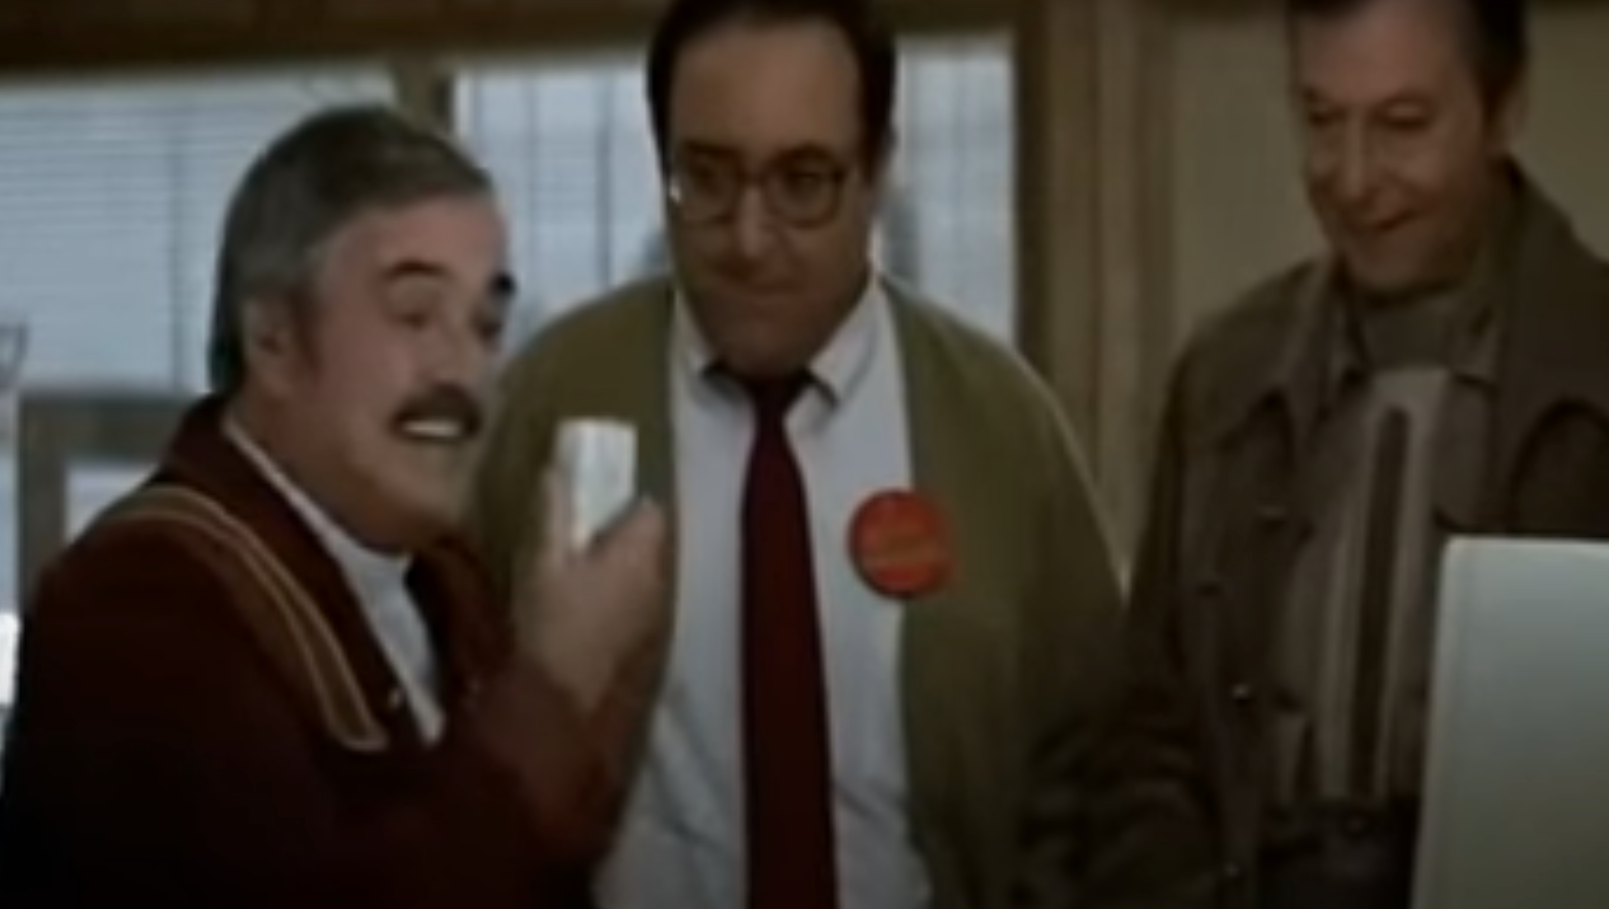
\includegraphics{www/scotty-computer.png}{]}{]}(https://www.youtube.com/embed/hShY6xZWVGE?si=bitLcj6fhMxUiO02)

Click link to play movie clip.

\end{footnotesize}}

``Walk the dog!'' has both a verb (``walk'') and a noun (``the dog'').
The noun in such an imperative is the \textbf{object} of the verb; the
entity that the action (walk) is to be applied to.

R structures sentences/commands differently. Every sentence is a
command. The actor is always the computer, there's no reason to state
that explicitly. So the imperative in R looks like this:

\texttt{the\_dog\ \textbar{}\textgreater{}\ walk}

In word order, the object of the action \emph{preceeds} the action. In
data-wrangling commands, the object is always a data frame.

\end{tcolorbox}

\subsection{Pivoting (optional)}\label{pivoting-optional}

In an earlier example, we used \texttt{mutate()} to compute a new column
called \texttt{GDPpercap} by dividing two existing columns, \texttt{GDP}
and \texttt{pop}. With \texttt{mutate()}, it's easy to do calculations
that involve two or more columns within the same row.

Now consider a similar sounding task, computing \texttt{GDPgrowth} by
dividing, for each country separately, the 2020 GDP with the 1950 GDP.
This cannot be done with a simple \texttt{mutate()} step because the
information needed for the calculation is spread over two different
rows. A clue to the difficulty is that there are not separate columns
named, say, \texttt{GDP2020} and \texttt{GDP1950} that could be combined
with a \texttt{mutate()} operation.

``\textbf{Pivoting}'' is a data wrangling operation that reshapes a data
frame. Understanding pivoting is essential for the professional data
scientist. But, like the construction of compound wrangling statements
in general, mastery comes with experience. You won't need to master
pivot to study these \emph{Lessons}, but we do use it behind the scenes
in some of the demonstrations. Mainly, it's worthwhile to learn a little
about pivoting in order better to appreciate how data wrangling uses a
small number of general-purpose operations to accomplish a huge variety
of tasks.

Consider a data frame for which you want to turn information in
different rows into a format with that information in different columns.
That is, we're going to take information from a single column in the
original, and spread it between two (or more) columns in the output from
the operation. Adding columns is effectively making a data frame
``\textbf{wider}.'' We can accomplish the \texttt{GDPgrowth} wrangling
by pivoting from ``\textbf{longer}'' (that is, more rows) to
``\textbf{wider}''. Like this:

\begin{Shaded}
\begin{Highlighting}[]
\NormalTok{Nats }\SpecialCharTok{|\textgreater{}} \FunctionTok{pivot\_wider}\NormalTok{(country, }\AttributeTok{values\_from =} \FunctionTok{c}\NormalTok{(GDP, pop), }\AttributeTok{names\_from =}\NormalTok{ year)}
\end{Highlighting}
\end{Shaded}

\begin{verbatim}


| country | GDP_2020 | GDP_1950 | pop_2020 | pop_1950 |
|:-------:|:--------:|:--------:|:--------:|:--------:|
|  Korea  |   874    |   100    |    32    |    32    |
|  Cuba   |    80    |    60    |    7     |    8     |
| France  |   1203   |   250    |    55    |    40    |
|  India  |   1100   |   300    |   1300   |   700    |
\end{verbatim}

This is a complicated command, so we will break it down argument by
argument.

\begin{enumerate}
\def\labelenumi{\arabic{enumi}.}
\item
  The first argument, \texttt{country}, specifies the variable values
  that will label each row in the result. Even though \texttt{country}
  has eight values, there are only four distinct values so the result
  will have four rows.
\item
  The second argument, \texttt{values\_from\ =\ c(GDP,\ pop)}, tells
  which columns we are going to make wider. Here, we are creating
  side-by-side columns for both \texttt{GDP} and \texttt{pop}.
\item
  The third argument, \texttt{names\_from\ =\ year}, tells what variable
  in the original will spread of the columns in the second argument.
  Since \texttt{year} has two distinct values (1950 and 2020), the
  \texttt{values\_from} columns will be split into two columns each. If
  year had three distinct values (say, 1980 as well as 1950 and 2020),
  then the splitting would be into three columns for each of the
  \texttt{values\_from} columns. :::
\end{enumerate}

The pivoted data contains the same information as the original, but
organized differently. The new organization makes it easy to do the
\texttt{GDPgrowth} calculation, since now it is just the ratio of two
columns:

\begin{Shaded}
\begin{Highlighting}[]
\NormalTok{Nats }\SpecialCharTok{|\textgreater{}} 
  \FunctionTok{pivot\_wider}\NormalTok{(country, }\AttributeTok{values\_from =} \FunctionTok{c}\NormalTok{(GDP, pop), }\AttributeTok{names\_from =}\NormalTok{ year) }\SpecialCharTok{|\textgreater{}}
  \FunctionTok{mutate}\NormalTok{(}\AttributeTok{GDP\_growth =}\NormalTok{ GDP\_2020 }\SpecialCharTok{/}\NormalTok{ GDP\_1950) }\SpecialCharTok{|\textgreater{}}
  \FunctionTok{select}\NormalTok{(country, GDP\_growth)}
\end{Highlighting}
\end{Shaded}

\begin{verbatim}


| country | GDP_growth |
|:-------:|:----------:|
|  Korea  |    8.74    |
|  Cuba   |   1.333    |
| France  |   4.812    |
|  India  |   3.667    |
\end{verbatim}

As you might suspect, there is also a \texttt{pivot\_longer()}
operation, which merges columns rather than spreading them.

\begin{tcolorbox}[enhanced jigsaw, colbacktitle=quarto-callout-note-color!10!white, opacityback=0, breakable, opacitybacktitle=0.6, colback=white, coltitle=black, arc=.35mm, title=\textcolor{quarto-callout-note-color}{\faInfo}\hspace{0.5em}{Exercise 5.27 Q05-113}, left=2mm, colframe=quarto-callout-note-color-frame, rightrule=.15mm, bottomrule=.15mm, leftrule=.75mm, bottomtitle=1mm, toptitle=1mm, titlerule=0mm, toprule=.15mm]

DRAFT

I want to do some things with babynames, but I have to keep them simple.

NOTE IN DRAFT: Move this to a section for more advanced exercises:
perhaps Mini-Projects.

See Z-cat-wear-canoe.qmd

\end{tcolorbox}

\begin{tcolorbox}[enhanced jigsaw, colbacktitle=quarto-callout-note-color!10!white, opacityback=0, breakable, opacitybacktitle=0.6, colback=white, coltitle=black, arc=.35mm, title=\textcolor{quarto-callout-note-color}{\faInfo}\hspace{0.5em}{Exercise 5.28 Q05-114}, left=2mm, colframe=quarto-callout-note-color-frame, rightrule=.15mm, bottomrule=.15mm, leftrule=.75mm, bottomtitle=1mm, toptitle=1mm, titlerule=0mm, toprule=.15mm]

DRAFT

Compute the mother's weight gain during pregnancy as indicated by
\texttt{natality2014::Natality\_2014\_100k} and graph it versus baby's
weight \texttt{dbwt}. Is there an obvious relationship between the two
variables? CHANGE THIS TO \texttt{Births2022} where the variables are
\texttt{weight\_pre}, \texttt{weight\_delivery}, \texttt{weight}.

\end{tcolorbox}

\begin{tcolorbox}[enhanced jigsaw, colbacktitle=quarto-callout-note-color!10!white, opacityback=0, breakable, opacitybacktitle=0.6, colback=white, coltitle=black, arc=.35mm, title=\textcolor{quarto-callout-note-color}{\faInfo}\hspace{0.5em}{Exercise 5.29 Q05-115}, left=2mm, colframe=quarto-callout-note-color-frame, rightrule=.15mm, bottomrule=.15mm, leftrule=.75mm, bottomtitle=1mm, toptitle=1mm, titlerule=0mm, toprule=.15mm]

DRAFT

Average family size from the child's point of view and from the
households point of view.

\end{tcolorbox}

\begin{tcolorbox}[enhanced jigsaw, colbacktitle=quarto-callout-note-color!10!white, opacityback=0, breakable, opacitybacktitle=0.6, colback=white, coltitle=black, arc=.35mm, title=\textcolor{quarto-callout-note-color}{\faInfo}\hspace{0.5em}{Exercise 5.30 Q05-116}, left=2mm, colframe=quarto-callout-note-color-frame, rightrule=.15mm, bottomrule=.15mm, leftrule=.75mm, bottomtitle=1mm, toptitle=1mm, titlerule=0mm, toprule=.15mm]

DRAFT

\texttt{Parents} is just one of the reasonable formats for storing the
parent data. Another perfectly good format would have the unit of
observation be an individual parent rather than a mother/father pair.

\texttt{\{r\ echo=FALSE,\ \ eval=FALSE\}\ \#\textbar{}\ label:\ tbl-parent\ \#\textbar{}\ tbl-cap:\ "The\ \textasciigrave{}Parent\textasciigrave{}\ (singular)\ data\ frame\ where\ the\ unit\ of\ observation\ is\ an\ individual\ parent."\ \#\textbar{}\ tbl-cap-location:\ margin\ Parents\ \textbar{}\textgreater{}\ pivot\_longer(cols\ =\ c("mother",\ "father"),\ values\_to\ =\ "parent\_height",\ names\_to\ =\ "role")}

\end{tcolorbox}

\begin{tcolorbox}[enhanced jigsaw, colbacktitle=quarto-callout-note-color!10!white, opacityback=0, breakable, opacitybacktitle=0.6, colback=white, coltitle=black, arc=.35mm, title=\textcolor{quarto-callout-note-color}{\faInfo}\hspace{0.5em}{Exercise 5.31 Q05-104}, left=2mm, colframe=quarto-callout-note-color-frame, rightrule=.15mm, bottomrule=.15mm, leftrule=.75mm, bottomtitle=1mm, toptitle=1mm, titlerule=0mm, toprule=.15mm]

SORTING EXERCISES, including sorting in descending order.

\end{tcolorbox}

\begin{tcolorbox}[enhanced jigsaw, colbacktitle=quarto-callout-note-color!10!white, opacityback=0, breakable, opacitybacktitle=0.6, colback=white, coltitle=black, arc=.35mm, title=\textcolor{quarto-callout-note-color}{\faInfo}\hspace{0.5em}{Exercise 5.32 Q05-105}, left=2mm, colframe=quarto-callout-note-color-frame, rightrule=.15mm, bottomrule=.15mm, leftrule=.75mm, bottomtitle=1mm, toptitle=1mm, titlerule=0mm, toprule=.15mm]

FILTERING EXERCISES

Include \texttt{\%in\%}

\end{tcolorbox}

\begin{tcolorbox}[enhanced jigsaw, colbacktitle=quarto-callout-note-color!10!white, opacityback=0, breakable, opacitybacktitle=0.6, colback=white, coltitle=black, arc=.35mm, title=\textcolor{quarto-callout-note-color}{\faInfo}\hspace{0.5em}{Exercise 5.33 panda-sleep-cotton}, left=2mm, colframe=quarto-callout-note-color-frame, rightrule=.15mm, bottomrule=.15mm, leftrule=.75mm, bottomtitle=1mm, toptitle=1mm, titlerule=0mm, toprule=.15mm]

```\{r label=`Z-panda-sleep-cottonOE4ul6', include = FALSE\}
set.seed(102)

Big \textless- babynames::babynames \%\textgreater\% filter( n
\textgreater{} 500 )

theseNames \textless- unique(Big \%\textgreater\% sample\_n(size =
10)){[}{[}``name''{]}{]} \%\textgreater\% head( 3 )

One \textless- babynames::babynames \textbar\textgreater{} filter( name
\%in\% theseNames, year \%in\% c(1912,2012)) \textbar\textgreater{}
summarize( nbabies=sum(n), .by = c(name, sex, year))
\textbar\textgreater{} arrange(year) \textbar\textgreater{} tail(10)

Two \textless- One \textbar\textgreater{} spread( key=sex,
value=nbabies, fill = 0 )

Three \textless- One \textbar\textgreater{} spread( key=year,
value=nbabies, fill = 0 )

Four \textless- One \textbar\textgreater{} spread( key=name,
value=nbabies, fill = 0)

options( xtable.NA.string = ``NA'' )

Five \textless- Four \textbar\textgreater{} spread(key=sex, value=year )

\begin{verbatim}


Consider the following forms for organizing a subset of the `babynames::babynames`.
    
```{r panda-sleep-cotton-1,  echo=FALSE, caption="Version One"}
One 
\end{verbatim}

\texttt{\{r\ panda-sleep-cotton-3,\ echo=FALSE,\ caption="Version\ Two"\}\ Two}

\texttt{\{r\ panda-sleep-cotton-4,\ echo=FALSE,\ caption="Version\ Three"\}\ Three}

\begin{enumerate}
\def\labelenumi{\arabic{enumi}.}
\item
  Do all three forms represent the same set of facts?
  \texttt{r\ short\_answer(r"-\/-(Yes.\ For\ instance,\ from\ all\ three\ forms\ you\ can\ see\ that\ in\ 1912\ there\ were\ 8764\ baby\ girls\ and\ 22\ baby\ boys\ given\ the\ name\ Mildred.)-\/-")}
\item
  What is the meaning of a row in each of the tables?

  \begin{itemize}
  \tightlist
  \item
    Version One
    \texttt{r\ short\_answer(r"-\/-(A\ name\ given\ to\ babies\ of\ a\ specific\ sex\ in\ a\ specific\ year)-\/-")}
  \item
    Version Two
    \texttt{r\ short\_answer(r"-\/-(A\ name\ in\ a\ year)-\/-")}
  \item
    Version Three
    \texttt{r\ short\_answer(r"-\/-(A\ name\ given\ to\ a\ sex\ \ \ )-\/-")}
  \end{itemize}
\item
  Which form of table makes it easiest to calculate the ratio of male to
  female in each name in each year?
  \texttt{r\ short\_answer(r"-\/-(For\ Two.\ A\ simple\ application\ of\ \textbackslash{}tt\{mutate()\}\ can\ calculate\ the\ ratio.)-\/-")}
\item
  There are no zeroes in Version One, but there are in Versions Two and
  Three. Why?
  \texttt{r\ short\_answer(r"-\/-(In\ version\ Two,\ there\ is\ a\ slot\ for\ every\ combination\ of\ name\ and\ year\ and\ sex,\ even\ when\ the\ count\ of\ babies\ is\ zero,\ whereas\ version\ One\ only\ has\ slots\ for\ non-zero\ counts\ of\ the\ count\ of\ babies.\ )-\/-")}
\item
  Version Three was ``spread'' from Version One. What variable sets the
  spread columns?
  \texttt{r\ short\_answer(r"-\/-(\textbackslash{}tt\{year\})-\/-")}
\end{enumerate}

\end{tcolorbox}

\begin{tcolorbox}[enhanced jigsaw, colbacktitle=quarto-callout-note-color!10!white, opacityback=0, breakable, opacitybacktitle=0.6, colback=white, coltitle=black, arc=.35mm, title=\textcolor{quarto-callout-note-color}{\faInfo}\hspace{0.5em}{Exercise 5.34 kid-bend-dish}, left=2mm, colframe=quarto-callout-note-color-frame, rightrule=.15mm, bottomrule=.15mm, leftrule=.75mm, bottomtitle=1mm, toptitle=1mm, titlerule=0mm, toprule=.15mm]

Use the \texttt{DataComputing::ZipGeography} and
\texttt{DataComputing::ZipDemography} data tables to create these
graphics.

\begin{enumerate}
\tightlist
\item
  Call a ZIP code ``crowded'' when the population is over 50,000. Make a
  point plot showing the geographic location of the crowded ZIPs.\\
\item
  Pick out the 10,000 zip codes with the highest population. Make a
  point plot of the latitude versus longitude. (Hints:
  \texttt{arrange()} and \texttt{head()}.) Use color to represent the
  fraction of the population that is over 65.\\
\item
  How many zip codes have a \texttt{WaterArea} that is more than 50\% of
  the \texttt{LandArea}? Make a point plot showing the geographical
  location of these, with color indicating the population.
\end{enumerate}

\end{tcolorbox}

\begin{tcolorbox}[enhanced jigsaw, colbacktitle=quarto-callout-note-color!10!white, opacityback=0, breakable, opacitybacktitle=0.6, colback=white, coltitle=black, arc=.35mm, title=\textcolor{quarto-callout-note-color}{\faInfo}\hspace{0.5em}{Exercise 5.35 doe-dream-room}, left=2mm, colframe=quarto-callout-note-color-frame, rightrule=.15mm, bottomrule=.15mm, leftrule=.75mm, bottomtitle=1mm, toptitle=1mm, titlerule=0mm, toprule=.15mm]

Using the \texttt{DataComputing::ZipGeography} data table, answer the
following questions. In addition to the answer itself, show the
statement that you used and the data table created by your statement
that contains the answer.

\begin{enumerate}
\def\labelenumi{\arabic{enumi}.}
\tightlist
\item
  How many different counties are there? (Hint: Use
  \texttt{n\_distinct()} within \texttt{summarize()}, but be careful
  what variable(s) you group by.)
\item
  Which city names are used in the most states?
\item
  Identify cities that include more than 5\% of their state population;
  which of those city names are used in the most states?
\item
  Does any state have more than one time zone?
\item
  Does any city have more than one time zone?
\item
  Does any county have more than one time zone?
\end{enumerate}

\end{tcolorbox}

\begin{tcolorbox}[enhanced jigsaw, colbacktitle=quarto-callout-note-color!10!white, opacityback=0, breakable, opacitybacktitle=0.6, colback=white, coltitle=black, arc=.35mm, title=\textcolor{quarto-callout-note-color}{\faInfo}\hspace{0.5em}{Exercise 5.36 seaweed-tug-kayak}, left=2mm, colframe=quarto-callout-note-color-frame, rightrule=.15mm, bottomrule=.15mm, leftrule=.75mm, bottomtitle=1mm, toptitle=1mm, titlerule=0mm, toprule=.15mm]

Imagine a data table, \texttt{Patients}, with categorical variables
\texttt{name}, \texttt{diagnosis}, \texttt{sex}, and quantitative
variable \texttt{age}.

You have a statement in the form

\begin{Shaded}
\begin{Highlighting}[]
\NormalTok{Patients }\SpecialCharTok{\%\textgreater{}\%}
  \FunctionTok{summarise}\NormalTok{(}\AttributeTok{count =} \FunctionTok{n}\NormalTok{(), }\AttributeTok{meanAge =} \FunctionTok{mean}\NormalTok{(age), }
            \AttributeTok{.by =} \SpecialCharTok{**}\NormalTok{SOME\_VARIABLES}\SpecialCharTok{**}\NormalTok{)}
\end{Highlighting}
\end{Shaded}

Replacing \texttt{**SOME\_VARIABLES**} with each of the following, tell
what variables will appear in the output

\begin{enumerate}
\def\labelenumi{\alph{enumi}.}
\tightlist
\item
  \texttt{sex}
\item
  \texttt{diagnosis}
\item
  c(\texttt{sex}, \texttt{diagnosis})
\item
  c(\texttt{age}, \texttt{diagnosis})
\item
  \texttt{age}
\end{enumerate}

\texttt{r\ long\_answer()}

The variables given as arguments to \texttt{.by\ =} will always appear
in the output, along with whatever variables are created by
\texttt{summarise()}.

\begin{enumerate}
\def\labelenumi{\alph{enumi}.}
\tightlist
\item
  \texttt{sex}, \texttt{count}, \texttt{meanAge}
\item
  \texttt{diagnosis}, \texttt{count}, \texttt{meanAge}
\item
  \texttt{sex}, \texttt{diagnosis}, \texttt{count}, \texttt{meanAge}
\item
  \texttt{age}, \texttt{diagnosis},\texttt{count}, \texttt{meanAge}
\item
  \texttt{age}, \texttt{count}, \texttt{meanAge}
\end{enumerate}

\texttt{r\ end\_long\_answer()}

\end{tcolorbox}

\begin{tcolorbox}[enhanced jigsaw, colbacktitle=quarto-callout-note-color!10!white, opacityback=0, breakable, opacitybacktitle=0.6, colback=white, coltitle=black, arc=.35mm, title=\textcolor{quarto-callout-note-color}{\faInfo}\hspace{0.5em}{Exercise 5.37 snail-sing-knife}, left=2mm, colframe=quarto-callout-note-color-frame, rightrule=.15mm, bottomrule=.15mm, leftrule=.75mm, bottomtitle=1mm, toptitle=1mm, titlerule=0mm, toprule=.15mm]

Each of these tasks can be performed using a single data verb. For each
task, say which verb it is:

\begin{enumerate}
\def\labelenumi{\arabic{enumi}.}
\tightlist
\item
  Add a new column that is the ratio between two variables.
  \texttt{r\ short\_answer(r"-\/-(\textbackslash{}tt\{mutate()\}\ )-\/-")}
\item
  Sort the cases in descending order of a
  variable.\texttt{r\ short\_answer(r"-\/-(\textbackslash{}tt\{arrange()\}\ \ )-\/-")}
\item
  Create a new data table that includes only those cases that meet a
  criterion.
  \texttt{r\ short\_answer(r"-\/-(\textbackslash{}tt\{filter()\})-\/-")}
\item
  From a data table with three categorical variables A, B, \& C, and a
  quantitative variable X, produce an output that has the same cases but
  only the variables A and X.
  \texttt{r\ short\_answer(r"-\/-(\textbackslash{}tt\{select()\}\ )-\/-")}
\item
  From a data table with three categorical variables A, B, \& C, and a
  quantitative variable X, produce an output that has a separate case
  for each of the combinations of the levels of A and B.
  \texttt{r\ short\_answer(r"-\/-(\textbackslash{}tt\{summarise()\}\ using\ \textbackslash{}tt\{.by\ =\ c(A,\ B)\})-\/-")}
\end{enumerate}

\end{tcolorbox}

\begin{tcolorbox}[enhanced jigsaw, colbacktitle=quarto-callout-note-color!10!white, opacityback=0, breakable, opacitybacktitle=0.6, colback=white, coltitle=black, arc=.35mm, title=\textcolor{quarto-callout-note-color}{\faInfo}\hspace{0.5em}{Exercise 5.38 squirrel-by-rug}, left=2mm, colframe=quarto-callout-note-color-frame, rightrule=.15mm, bottomrule=.15mm, leftrule=.75mm, bottomtitle=1mm, toptitle=1mm, titlerule=0mm, toprule=.15mm]

```\{r squirrel-buy-rug-default, include = FALSE\} \# some row
calculations for chunk specs BabyNames\_All \textless-
babynames::babynames \textbar\textgreater{} nrow()

BabyNames\_F \textless- babynames::babynames \textbar\textgreater{}
filter(sex == ``F'') \textbar\textgreater{} nrow()

BabyNames\_M \textless- babynames::babynames \textbar\textgreater{}
filter(sex == ``M'') \textbar\textgreater{} nrow()

\begin{verbatim}

TITLE GOES HERE: Here is a reminder  of what the `BabyNames` data frame looks like. Take this table as the input to the data wranging statement you will construct.   

```{r squirrel-buy-rug-1, echo=FALSE, and_so_on= paste0("... and so on for ", BabyNames_All, " rows altogether.")}
set.seed( 102 )
Small <- sample_n( babynames::babynames, size = 10 )
row.names( Small ) <- NULL
Small 
\end{verbatim}

For each of the following outputs, identify the data verb linking the
input to the output and write down the details (i.e., arguments) of the
operation. (Hints: Look at the number of cases. The order of variables
may also be a clue.)

\begin{enumerate}
\def\labelenumi{\arabic{enumi}.}
\tightlist
\item
  Output Table A
\end{enumerate}

\texttt{\{r\ squirrel-buy-rug-A,\ echo=FALSE,\ and\_so\_on=\ paste0("...\ and\ so\ on\ for\ ",\ BabyNames\_All,\ "\ rows\ altogether.")\}\ Small\ \textbar{}\textgreater{}\ dplyr::arrange(sex,\ n\ )}

\begin{enumerate}
\def\labelenumi{\arabic{enumi}.}
\setcounter{enumi}{1}
\tightlist
\item
  Output Table B
\end{enumerate}

\texttt{\{r\ squirrel-buy-rug-B,\ \ echo=FALSE,\ and\_so\_on=\ paste0("...\ and\ so\ on\ for\ ",\ BabyNames\_F,\ "\ rows\ altogether.")\}\ Small\ \textbar{}\textgreater{}\ filter(sex\ ==\ "F"\ )}

\begin{enumerate}
\def\labelenumi{\arabic{enumi}.}
\setcounter{enumi}{2}
\tightlist
\item
  Output Table C
\end{enumerate}

\texttt{\{r\ squirrel-buy-rug-C,\ echo=FALSE,\ and\_so\_on=\ paste0("...\ and\ so\ on\ for\ ",\ BabyNames\_M,\ "\ rows\ altogether.")\}\ Small\ \textbar{}\textgreater{}\ filter(sex\ ==\ "M")}

\begin{enumerate}
\def\labelenumi{\arabic{enumi}.}
\setcounter{enumi}{3}
\tightlist
\item
  Output Table D
\end{enumerate}

\texttt{\{r\ squirrel-buy-rug-D,\ echo=FALSE\}\ babynames::babynames\ \textbar{}\textgreater{}\ summarise(total\ =\ sum(n)\ )}

\begin{enumerate}
\def\labelenumi{\arabic{enumi}.}
\setcounter{enumi}{4}
\tightlist
\item
  Output Table E
\end{enumerate}

\texttt{\{r\ squirrel-buy-rug-E,\ echo=FALSE,\ nrow=BabyNames\_All\}\ Small\ \textbar{}\textgreater{}\ select(name,\ n\ )}

\texttt{r\ long\_answer()}

\begin{enumerate}
\def\labelenumi{\alph{enumi}.}
\tightlist
\item
  \texttt{arrange(sex,\ n)}
\item
  \texttt{filter(sex\ ==\ "F")}
\item
  \texttt{filter(sex\ ==\ "M",\ n\ \textgreater{}\ 10)}
\item
  \texttt{summarise(total\ =\ sum(n))}
\item
  \texttt{select(name,\ n)}
\end{enumerate}

\texttt{r\ end\_long\_answer()}

\end{tcolorbox}

::::

\newpage

\section{Computing with functions and
arguments}\label{sec-data-computing}

You have already seen the R command patterns that we will use throughout
these \emph{Lessons}: pipelines composed of actions separated by
\texttt{\textbar{}\textgreater{}}, named data frames, functions and
their arguments. This Lesson recapitulates and explains those patterns,
the better to help you construct your own commands. The Lesson also
emphasizes a small technical vocabulary that helps in communicating with
other people to share insights and identify errors.

Learning command patterns is a powerful enabler in statistical thinking.
The computer is an indispensable tool for statistical thinking.
{\marginnote{\begin{footnotesize}This
\href{https://dtkaplan.github.io/Math300blog/posts/Indispensible-tool/}{blog
post} gives a little history of the long-standing link between
statistics and computing.\end{footnotesize}}} In addition to doing the
work of calculations, computer software is a medium for describing and
sharing with others statistical techniques and concepts. For instance,
three fundamental operations in statistics---randomize, repeat,
collect---are easily written in computer languages but have no
counterpart in the algebraic notation traditionally uused in mathematics
education.

\subsection{Chain of operations}\label{chain-of-operations}

A typical computing task consists of a chain of operations. For
instance, each wrangling operation receives a data-frame object from an
incoming pipe \texttt{\textbar{}\textgreater{}}, operates on that data
frame to perform the action described by the function's name and
arguments, and produces another data frame as output. Depending on the
overall task, the output from the operation may be piped into another
action or displayed on the screen.

There are also operations, like \texttt{point\_plot()}, that translate a
data frame into another kind of object: a \emph{graphic}. Starting with
Lesson \ref{sec-regression}, we will work with \texttt{model\_train()},
a function that translates a data frame into a \emph{model}. In this
Lesson, we will meet two other ways of dealing with the output of a
chain of operations: storing the output under a name for later use and
formatting a data frame into a table suited to human readers.

Manufacturing processes provide a helpful analogy for understanding the
step-by-step structure of a computation. Simple manufacturing processes
might involve one or a handful of work steps arranged in a chain.
Complex operations can involve many chains coming together in elaborate
configurations. The video in Figure~\ref{fig-pencil-video} shows the
steps of pencil manufacturing. These involves several inputs:

\begin{marginfigure}

\centering{

\url{https://www.youtube.com/embed/qqs3fxfmWr4}

}

\caption{\label{fig-pencil-video}Manufacturing a pencil, step by step.}

\end{marginfigure}%

The overall manufacturing process takes several inputs that are shaped
and combined to produce the pencil: cedar wood slabs, glue, graphite,
enamel paint Each input is processed in a step-by-step manner. At some
steps, two partially processed components are combined. For instance,
there is a step that grooves the cedar slabs (which are sourced from
another production line). The next step put glue in the groves. In still
another step, the graphite rods (which come from their own production
process) are placed into the glue-filled groves. (Lesson
\ref{sec-databases} introduces the data-wrangling process, join, that
combines two inputs.)

There are several different forms of conveyors in the pencil
manufacturing line that carry the materials from one manufacturing step
to the next. We need only one type of conveyor---the \textbf{pipe}---to
connect computing steps.

Manufacturing processes often involve storage or delivery. The video in
Figure~\ref{fig-pencil-video} ends before the final steps in the
process: boxing the pencils, warehousing them, and the parts of the
chain that deliver them to the consumer end-user.Storage, retrieval, and
customer use all have their counterparts in computing processes. By
default, the object produced by the computing chain is directly
delivered to the customer, here by displaying it in some appropriate
place, for instance directly under the computer command, or in a viewing
panel or document:

\begin{Shaded}
\begin{Highlighting}[]
\NormalTok{Nats }\SpecialCharTok{|\textgreater{}}
  \FunctionTok{mutate}\NormalTok{(}\AttributeTok{GDPpercap =}\NormalTok{ GDP }\SpecialCharTok{/}\NormalTok{ pop) }\SpecialCharTok{|\textgreater{}}
  \FunctionTok{filter}\NormalTok{(GDPpercap }\SpecialCharTok{\textgreater{}} \FunctionTok{mean}\NormalTok{(GDPpercap), }\AttributeTok{.by =}\NormalTok{ year)}
\end{Highlighting}
\end{Shaded}

\begin{verbatim}


| country | year | GDP  | pop | GDPpercap |
|:-------:|:----:|:----:|:---:|:---------:|
|  Korea  | 2020 | 874  | 32  |   27.31   |
| France  | 2020 | 1203 | 55  |   21.87   |
|  Cuba   | 1950 |  60  |  8  |    7.5    |
| France  | 1950 | 250  | 40  |   6.25    |
\end{verbatim}

In our computer notation, the storage operation can look like this:

\begin{Shaded}
\begin{Highlighting}[]
\NormalTok{Nats }\SpecialCharTok{|\textgreater{}}
  \FunctionTok{mutate}\NormalTok{(}\AttributeTok{GDPpercap =}\NormalTok{ GDP }\SpecialCharTok{/}\NormalTok{ pop) }\SpecialCharTok{|\textgreater{}}
  \FunctionTok{filter}\NormalTok{(GDPpercap }\SpecialCharTok{\textgreater{}} \FunctionTok{mean}\NormalTok{(GDPpercap), }\AttributeTok{.by=}\NormalTok{year) }\OtherTok{{-}\textgreater{}}\NormalTok{ High\_income\_countries}
\end{Highlighting}
\end{Shaded}

At the very end of the pipeline chain, there is a \textbf{storage arrow}
(\texttt{-\textgreater{}}, as opposed to the pipe,
\texttt{\textbar{}\textgreater{}}) followed by a \textbf{storage name}
(\texttt{High\_income\_countries}). The effect is to place the object at
the output end of the chain to be stored in computer memory in a
location identified by the storage name.

{\marginnote{\begin{footnotesize}\href{https://dtkaplan.github.io/Math300blog/posts/Idiom/index.html\#sec-storage-arrow}{Why
do you say \ldots?}\end{footnotesize}}}

Retrieval from storage is even simpler: just use the storage name as an
input. For instance:

\begin{Shaded}
\begin{Highlighting}[]
\NormalTok{High\_income\_countries }\SpecialCharTok{|\textgreater{}} 
  \FunctionTok{select}\NormalTok{(}\SpecialCharTok{{-}}\NormalTok{GDP, }\SpecialCharTok{{-}}\NormalTok{pop) }\SpecialCharTok{|\textgreater{}} 
  \FunctionTok{filter}\NormalTok{(year }\SpecialCharTok{==} \DecValTok{2020}\NormalTok{) }\SpecialCharTok{|\textgreater{}} 
  \FunctionTok{kable}\NormalTok{(}\AttributeTok{digits=}\DecValTok{2}\NormalTok{)}
\end{Highlighting}
\end{Shaded}

\begin{tabular}{l|r|r}
\hline
country & year & GDPpercap\\
\hline
Korea & 2020 & 27.31\\
\hline
France & 2020 & 21.87\\
\hline
\end{tabular}

\begin{tcolorbox}[enhanced jigsaw, colbacktitle=quarto-callout-note-color!10!white, opacityback=0, breakable, opacitybacktitle=0.6, colback=white, coltitle=black, arc=.35mm, title=\textcolor{quarto-callout-note-color}{\faInfo}\hspace{0.5em}{Pointing out storage from the start}, left=2mm, colframe=quarto-callout-note-color-frame, rightrule=.15mm, bottomrule=.15mm, leftrule=.75mm, bottomtitle=1mm, toptitle=1mm, titlerule=0mm, toprule=.15mm]

In a previous example we placed the storage arrow
(\texttt{-\textgreater{}}) at the end of a left-to-right chain of
operations. In practice, programmers and authors prefer another
arrangement---which we will use from now on in these
\emph{Lessons}---where the storage arrow is at the left end of the
chain. The storage arrow still points to the storage name. For instance,

\begin{Shaded}
\begin{Highlighting}[]
\NormalTok{High\_income\_countries }\OtherTok{\textless{}{-}}\NormalTok{ Nats }\SpecialCharTok{|\textgreater{}}
  \FunctionTok{mutate}\NormalTok{(}\AttributeTok{GDPpercap =}\NormalTok{ GDP }\SpecialCharTok{/}\NormalTok{ pop) }\SpecialCharTok{|\textgreater{}}
  \FunctionTok{filter}\NormalTok{(GDPpercap }\SpecialCharTok{\textgreater{}} \FunctionTok{mean}\NormalTok{(GDPpercap), }\AttributeTok{.by=}\NormalTok{year) }
\end{Highlighting}
\end{Shaded}

Using this \texttt{storage\_name\ \textless{}-} idiom it is easier to
scan code for storage names and to spot when the output of the chain is
to be delivered directly to the customer.

\end{tcolorbox}

\subsection{What's in a pipe?}\label{whats-in-a-pipe}

The pipe---that is, \texttt{\textbar{}\textgreater{}}---carries material
from one operation to another. In computer-speak, the word
``\textbf{object}'' describes this material. That is, pipes convey
objects.

Objects come in different ``\textbf{types}.'' Computer programmers learn
to deal with dozens of object types. Fortunately, we can accomplish what
we need in statistical computing with just a handful. You have already
met two types:

\begin{enumerate}
\def\labelenumi{\arabic{enumi}.}
\tightlist
\item
  data frames
\item
  graphics, consisting of one or more \textbf{layers}, e.g.~the point
  plot as one layer and the annotations as another layer placed on top.
\end{enumerate}

In later lessons, we will introduce two more types---(3) models and (4)
simulations.

\subsection{Pipes connect to
functions}\label{pipes-connect-to-functions}

At the receiving end of a pipe is an operation on the object conveyed by
the pipe. A better word for such an operation is ``\textbf{function}.''
It is easy to spot the functions in a pipeline: they \textbf{always}
consist of a name---such as \texttt{summarize} or
\texttt{point\_plot}---followed directly by \texttt{(} and, eventually,
a closing \texttt{)}. For example, in ::: \{.cell\}

\begin{Shaded}
\begin{Highlighting}[]
\NormalTok{Nats }\SpecialCharTok{|\textgreater{}}
  \FunctionTok{mutate}\NormalTok{(}\AttributeTok{GDPpercap =}\NormalTok{ GDP }\SpecialCharTok{/}\NormalTok{ pop) }\SpecialCharTok{|\textgreater{}}
  \FunctionTok{filter}\NormalTok{(GDPpercap }\SpecialCharTok{\textgreater{}} \FunctionTok{mean}\NormalTok{(GDPpercap), }\AttributeTok{.by =}\NormalTok{ year)}
\end{Highlighting}
\end{Shaded}

::: the first function is named \texttt{mutate}. The function output is
being piped to a second function, named \texttt{filter}. From now on,
whenever we name a function we will write the name followed by
\texttt{()} to remind the reader that the name refers to a function: so
\texttt{mutate()} and \texttt{filter()}. There are other things that
names can refer to. For instance, \texttt{Nats} at the start of the
pipeline is a data frame, and \texttt{GDP}, \texttt{GDPpercap} and
\texttt{pop}, and \texttt{year} are \emph{variables}. Such names for
non-functions are \textbf{never} followed directly by \texttt{(}.

\begin{tcolorbox}[enhanced jigsaw, colbacktitle=quarto-callout-note-color!10!white, opacityback=0, breakable, opacitybacktitle=0.6, colback=white, coltitle=black, arc=.35mm, title=\textcolor{quarto-callout-note-color}{\faInfo}\hspace{0.5em}{Example: What does \texttt{mean} refer to?}, left=2mm, colframe=quarto-callout-note-color-frame, rightrule=.15mm, bottomrule=.15mm, leftrule=.75mm, bottomtitle=1mm, toptitle=1mm, titlerule=0mm, toprule=.15mm]

Another name appearing in the previous code block is \texttt{mean}. What
kind of thing does this name refer to?

\begin{tcolorbox}[enhanced jigsaw, colbacktitle=quarto-callout-note-color!10!white, opacityback=0, breakable, opacitybacktitle=0.6, colback=white, coltitle=black, arc=.35mm, title=\textcolor{quarto-callout-note-color}{\faInfo}\hspace{0.5em}{Answer}, left=2mm, colframe=quarto-callout-note-color-frame, rightrule=.15mm, bottomrule=.15mm, leftrule=.75mm, bottomtitle=1mm, toptitle=1mm, titlerule=0mm, toprule=.15mm]

Because the name is directly followed by a parentheses, we know
\texttt{mean} must refer to a function.

Following our convention for writing function names, we should have
written the name as \texttt{mean()}, but that would have made the
question too easy!

\end{tcolorbox}

\end{tcolorbox}

\subsection{Arguments (inside the
parentheses)}\label{arguments-inside-the-parentheses}

Almost always when using a function the human writer of a computer
expression needs to specify some details of how the function is to work.
These details are \textbf{always} put inside the parentheses following
the name of the function. To illustrate, consider the task of plotting
the data in the \texttt{SAT} data frame. The \emph{skeleton} of the
computer command is

\begin{Shaded}
\begin{Highlighting}[]
\NormalTok{SAT }\SpecialCharTok{|\textgreater{}} \FunctionTok{point\_plot}\NormalTok{()}
\end{Highlighting}
\end{Shaded}

This skeleton is not a complete command, as becomes evident when the
(incomplete) command is evaluated:

\begin{Shaded}
\begin{Highlighting}[]
\NormalTok{SAT }\SpecialCharTok{|\textgreater{}} \FunctionTok{point\_plot}\NormalTok{()}
\end{Highlighting}
\end{Shaded}

\begin{verbatim}
Error in data_from_tilde(data, tilde): argument "tilde" is missing, with no default
\end{verbatim}

What's missing from the erroneous command is a detail needed to complete
the operation: What variables from \texttt{SAT} to map to y and x. This
detail is provided to \texttt{point\_plot()} as an argument. As you saw
in Lesson \ref{sec-point_plots}, the argument is written as a
\textbf{tilde expression}, for instance
\texttt{sat\ \textasciitilde{}\ frac} to map \texttt{sat} to y and
\texttt{frac} to x. Once we have constructed the appropriate argument
for the task at hand, we place it inside the parentheses that follow the
function name.

\begin{Shaded}
\begin{Highlighting}[]
\NormalTok{SAT }\SpecialCharTok{|\textgreater{}} \FunctionTok{point\_plot}\NormalTok{(sat }\SpecialCharTok{\textasciitilde{}}\NormalTok{ frac) }
\end{Highlighting}
\end{Shaded}

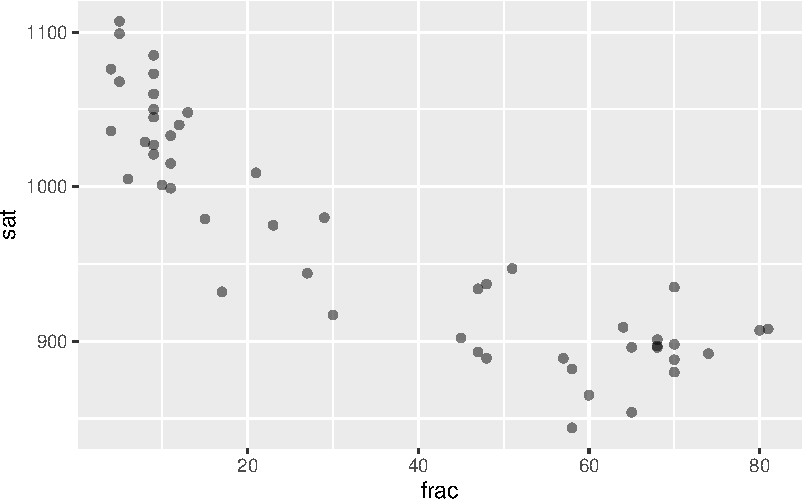
\includegraphics{test-tufte_files/figure-pdf/unnamed-chunk-84-1.pdf}

Many functions have more than one argument. Some arguments, like the
tilde expression argument to \texttt{point\_plot()}, may be required.
When an argument is not required, the argument itself is given a name
and it will have a \textbf{default value}. In the case of
\texttt{point\_plot()}, there is a second argument named \texttt{annot=}
to specify what kind of annotation layer to add on top of the point
plot. The default value of \texttt{annot=} turns off the annotation
layer.

\textbf{Named arguments}, like \texttt{annot=}, will \textbf{always} be
followed by a single equal sign, followed by the value to which that
argument is to be set. For instance, \texttt{point\_plot()} allows four
different values for \texttt{annot=}:

\begin{enumerate}
\def\labelenumi{\roman{enumi}.}
\tightlist
\item
  the default (which turns off the annotation)
\item
  \texttt{annot\ =\ "violin"} specifying a density display annotation
\item
  \texttt{annot\ =\ "bw"} which creates a traditional
  ``box-and-whiskers'' display of distribution that we will not use much
  in these lessons.
\item
  \texttt{annot\ =\ "model"} which annotates with a graph of a model
\end{enumerate}

In these Lessons, the single \texttt{=} sign always signifies a named
argument.
{\marginnote{\begin{footnotesize}\href{https://dtkaplan.github.io/Math300blog/posts/Idiom/index.html\#sec-equal-assignment}{Why
do you say \ldots?}\end{footnotesize}}}

A closely related use for \texttt{=} is to give a name to a calculated
result from \texttt{mutate()} or \texttt{summarize()}. For instance,
suppose you want to calculate the mean sat score and mean fraction in
the \texttt{SAT} data frame. This is easy:

\begin{Shaded}
\begin{Highlighting}[]
\NormalTok{SAT }\SpecialCharTok{|\textgreater{}} \FunctionTok{summarize}\NormalTok{(}\FunctionTok{mean}\NormalTok{(sat), }\FunctionTok{mean}\NormalTok{(frac))}
\end{Highlighting}
\end{Shaded}

\begin{longtable}[]{@{}cc@{}}
\toprule\noalign{}
mean(sat) & mean(frac) \\
\midrule\noalign{}
\endhead
\bottomrule\noalign{}
\endlastfoot
965.9 & 35.24 \\
\end{longtable}

We will often use this \emph{unnamed} style when the results are
intended for the human reader. But if such a calculation fed down the
pipeline to further calculations, it can be helpful to give simple names
to the result. Frivolously, we'll illustrate using the names
\texttt{eel} and \texttt{fish}:

\begin{Shaded}
\begin{Highlighting}[]
\NormalTok{SAT }\SpecialCharTok{|\textgreater{}} \FunctionTok{summarize}\NormalTok{(}\AttributeTok{eel =} \FunctionTok{mean}\NormalTok{(sat), }\AttributeTok{fish =} \FunctionTok{mean}\NormalTok{(frac))}
\end{Highlighting}
\end{Shaded}

\begin{longtable}[]{@{}cc@{}}
\toprule\noalign{}
eel & fish \\
\midrule\noalign{}
\endhead
\bottomrule\noalign{}
\endlastfoot
965.9 & 35.24 \\
\end{longtable}

The reason for the frivolity here is to point out that \emph{you} get to
choose the names for the results calculated by \texttt{mutate()} and
\texttt{summarize()}. Needless to say, it's best to avoid frivolous or
misleading names.

\subsection{Variable names in
arguments}\label{variable-names-in-arguments}

Many of the functions we use are on the receiving end of a pipe carrying
a data frame. Examples, perhaps already familiar to you:
\texttt{filter()}, \texttt{point\_plot()}, \texttt{mutate()}, and so on.

A good analogy for a data frame is a shipping box. Inside the shipping
box: one or more variables. When a function receives the \st{shipping
box} data frame, it opens it, providing access to each variable
contained therein. In constructing arguments to the function, you do not
have to think about the box, just the contents. You refer to the
contents only by their names. \texttt{select()} provides a good example,
since each argument can be simply the name of a variable, e.g.~

For most uses, the arguments to a function will be an expressions
constructed out of variable names. Some examples:

\begin{itemize}
\tightlist
\item
  \texttt{SAT\ \textbar{}\textgreater{}\ filter(frac\ \textgreater{}\ 50)}
  where the argument checks whether each value of \texttt{frac} is
  greater than 50.
\item
  \texttt{SAT\ \textbar{}\textgreater{}\ mutate(efficiency\ =\ sat\ /\ expend)}
  where the argument gives a name (\texttt{efficiency}) to an arithmetic
  combination of \texttt{sat} and \texttt{expend}.
\item
  \texttt{SAT\ \textbar{}\textgreater{}\ point\_plot(frac\ \textasciitilde{}\ expend)}
  where the argument to \texttt{point\_plot()} is an expression
  involving both \texttt{frac} and \texttt{expend}.
\item
  \texttt{SAT\ \textbar{}\textgreater{}\ filter(expend\ \textgreater{}\ median(expend))}
  where the argument involves calculating the median expenditure across
  the state using the \texttt{median()} reduction function, then
  comparing the calculated median to the actual expenditure in each
  state. The overall effect is to remove any state with a below-median
  expenditure from the output of \texttt{filter()}.
\item
  \texttt{SAT\ \textbar{}\textgreater{}\ select(-state,\ -frac)} uses
  the \texttt{-} sign to exclude the variables from the output.
\end{itemize}

\begin{tcolorbox}[enhanced jigsaw, colbacktitle=quarto-callout-warning-color!10!white, opacityback=0, breakable, opacitybacktitle=0.6, colback=white, coltitle=black, arc=.35mm, title=\textcolor{quarto-callout-warning-color}{\faExclamationTriangle}\hspace{0.5em}{Quotation marks}, left=2mm, colframe=quarto-callout-warning-color-frame, rightrule=.15mm, bottomrule=.15mm, leftrule=.75mm, bottomtitle=1mm, toptitle=1mm, titlerule=0mm, toprule=.15mm]

Sometimes, you will see an argument written as letters and numbers
\emph{inside} quotation marks, as in \texttt{annot\ =\ "model"}. The
quotation marks instruct the computer to take the contents literally
instead of pointing to a function or a variable. (In computer
terminology, the content of the quotation marks is called a
\textbf{character string}.)

The style of R commands does not use quotations around the names of
objects, functions, and variables are \textbf{not} placed in quotations.
When you see quotation marks in an example in these Lessons, take note.
They are needed, for instance, in saying what kind of annotation should
be drawn by \texttt{point\_plot()}. If you forget to use the quotation
marks where they are needed, the computer will signal an error:

\begin{Shaded}
\begin{Highlighting}[]
\NormalTok{Penguins }\SpecialCharTok{|\textgreater{}} \FunctionTok{point\_plot}\NormalTok{(bill\_length }\SpecialCharTok{\textasciitilde{}}\NormalTok{ flipper, }\AttributeTok{annot =}\NormalTok{ model) }
\end{Highlighting}
\end{Shaded}

\begin{verbatim}
Error in match.arg(annot): 'arg' must be NULL or a character vector
\end{verbatim}

The error message is terse, but it gives hints; for example,
\texttt{\textquotesingle{}arg\textquotesingle{}} suggests the error is
about an argument, \texttt{annot} is the name of the problematic
argument, and \texttt{character} is meant to point you to some issue
involving character strings.

\end{tcolorbox}

\subsection{Styling with space}\label{styling-with-space}

Written English uses space to separate words. It is helpful to the human
reader to follow analogous forms in R commands.

\begin{itemize}
\tightlist
\item
  Use spaces around storage arrows and pipes:
  \texttt{x\ \textless{}-\ 7\ \textbar{}\textgreater{}\ sqrt()} reads
  better than \texttt{x\textless{}-7\textbar{}\textgreater{}sqrt()}.
\item
  Use spaces between an argument name and its value:
  \texttt{mutate(percap\ =\ GDP\ /\ pop)} rather than
  \texttt{mutate(percap=GDP/pop)}.
\item
  When writing long pipelines, put a newline after the pipe symbol. You
  can see several instances of this in previous examples in this Lesson.
  DO NOT, however, start a line with a pipe symbol.
\end{itemize}

\subsection{Displaying tables}\label{sec-displaying-tables}

We are using the word ``\textbf{table}'' to refer specifically to a
printed display intended for a human reader, as opposed to data frames
which, although often readable, are oriented around computer memory.

The readability of tabular content goes beyond placing the content in
neatly aligned columns and rows to include the issue of the number of
``significant digits'' to present. All of the functions we use for
statistical computations make use of internal hardware that deals with
numbers to a precision of fifteen digits. Such precision is warranted
for internal calculations, which often build on one another. But fifteen
digits is much more than can be readily assimilated by the human reader.
To see why, let's display calculate yearly GDP growth (in percent) with
all the digits that are carried along in internal calculations:

\begin{Shaded}
\begin{Highlighting}[]
\NormalTok{Growth\_rate }\OtherTok{\textless{}{-}}\NormalTok{ Nats }\SpecialCharTok{|\textgreater{}} 
  \FunctionTok{pivot\_wider}\NormalTok{(country, }
              \AttributeTok{values\_from =} \FunctionTok{c}\NormalTok{(GDP, pop), }
              \AttributeTok{names\_from =}\NormalTok{ year) }\SpecialCharTok{|\textgreater{}}
  \FunctionTok{mutate}\NormalTok{(}\AttributeTok{yearly\_growth =} 
           \FloatTok{100.}\SpecialCharTok{*}\NormalTok{((GDP\_2020 }\SpecialCharTok{/}\NormalTok{ GDP\_1950)}\SpecialCharTok{\^{}}\NormalTok{(}\DecValTok{1}\SpecialCharTok{/}\FloatTok{70.}\NormalTok{)}\SpecialCharTok{{-}}\DecValTok{1}\NormalTok{)) }\SpecialCharTok{|\textgreater{}}
  \FunctionTok{select}\NormalTok{(country, yearly\_growth)}
\NormalTok{Growth\_rate}
\end{Highlighting}
\end{Shaded}

\begin{longtable}[]{@{}cc@{}}
\toprule\noalign{}
country & yearly\_growth \\
\midrule\noalign{}
\endhead
\bottomrule\noalign{}
\endlastfoot
Korea & 3.14547099309945 \\
Cuba & 0.411820047041944 \\
France & 2.26982406656688 \\
India & 1.87345150307259 \\
\end{longtable}

:::

GDP, like many quantities, can be measured only approximately. It would
be generous to ascribe a precision of about 1 part in 100 to GDP.
Informally, this suggests that only the first two or three digits of a
calculation based on GDP can have any real meaning.

The problem of significant digits has two parts: 1) how many digits are
worth displaying {\marginnote{\begin{footnotesize}We will take a
statistical view of the appropriate number of digits to show in
Chapter~\ref{sec-confidence-intervals}.\end{footnotesize}}} and 2) how
to instruct the computer to display only that number of digits. Point
(1) often depends on expert knowledge of a field. Point (2) is much more
straightforward; use a computer function that controls the number of
digits printed. There are many such functions. For simplicity, we focus
on one widely used in the R community, \texttt{kable()}.

The purpose of \texttt{kable()} can be described in plain English: to
format tabular output for the human reader. Whenever encountering a new
function, you will want to find out what are the \emph{inputs} and what
is the \emph{output}. The primary input to \texttt{kable()} is a data
frame. Additional arguments, if any, specify details of the formatting,
such as the number of digits to show. For instance:

\begin{Shaded}
\begin{Highlighting}[]
\NormalTok{Growth\_rate }\SpecialCharTok{|\textgreater{}} 
  \FunctionTok{kable}\NormalTok{(}\AttributeTok{digits =} \DecValTok{1}\NormalTok{, }
        \AttributeTok{caption =} \StringTok{"Annual growth in GDP from 1950 to 2020"}\NormalTok{,}
        \AttributeTok{col.names =} \FunctionTok{c}\NormalTok{(}\StringTok{""}\NormalTok{, }\StringTok{"Growth rate (\%)"}\NormalTok{))}
\end{Highlighting}
\end{Shaded}

\begin{table}

\caption{\label{tab:unnamed-chunk-90}Annual growth in GDP from 1950 to 2020}
\centering
\begin{tabular}[t]{l|r}
\hline
 & Growth rate (\%)\\
\hline
Korea & 3.1\\
\hline
Cuba & 0.4\\
\hline
France & 2.3\\
\hline
India & 1.9\\
\hline
\end{tabular}
\end{table}

The output of \texttt{kable()}, perhaps surprisingly, is \textbf{not} a
data frame. Instead, the output is instructions intended for the
display's typesetting facility. The typesetting instructions for
web-browsers are often written in a special-purpose language called
HTML. So far as these \emph{Lessons} are concerned, is not important
that you understand the HTML instructions. Even so, we show them to you
to emphasize an important point: You can't use the output of
\texttt{kable()} as the input to data-wrangling or graphics operation.

\begin{Shaded}
\begin{Highlighting}[]
\DataTypeTok{\textless{}}\KeywordTok{table}\DataTypeTok{\textgreater{}}
\DataTypeTok{\textless{}}\KeywordTok{caption}\DataTypeTok{\textgreater{}}\NormalTok{Annual growth in GDP from 1950 to 2020}\DataTypeTok{\textless{}/}\KeywordTok{caption}\DataTypeTok{\textgreater{}}
 \DataTypeTok{\textless{}}\KeywordTok{thead}\DataTypeTok{\textgreater{}}
  \DataTypeTok{\textless{}}\KeywordTok{tr}\DataTypeTok{\textgreater{}}
   \DataTypeTok{\textless{}}\KeywordTok{th}\OtherTok{ style}\OperatorTok{=}\StringTok{"text{-}align:left;"}\DataTypeTok{\textgreater{}}  \DataTypeTok{\textless{}/}\KeywordTok{th}\DataTypeTok{\textgreater{}}
   \DataTypeTok{\textless{}}\KeywordTok{th}\OtherTok{ style}\OperatorTok{=}\StringTok{"text{-}align:right;"}\DataTypeTok{\textgreater{}}\NormalTok{ Growth rate (\%) }\DataTypeTok{\textless{}/}\KeywordTok{th}\DataTypeTok{\textgreater{}}
  \DataTypeTok{\textless{}/}\KeywordTok{tr}\DataTypeTok{\textgreater{}}
 \DataTypeTok{\textless{}/}\KeywordTok{thead}\DataTypeTok{\textgreater{}}
\DataTypeTok{\textless{}}\KeywordTok{tbody}\DataTypeTok{\textgreater{}}
  \DataTypeTok{\textless{}}\KeywordTok{tr}\DataTypeTok{\textgreater{}}
   \DataTypeTok{\textless{}}\KeywordTok{td}\OtherTok{ style}\OperatorTok{=}\StringTok{"text{-}align:left;"}\DataTypeTok{\textgreater{}}\NormalTok{ Korea }\DataTypeTok{\textless{}/}\KeywordTok{td}\DataTypeTok{\textgreater{}}
   \DataTypeTok{\textless{}}\KeywordTok{td}\OtherTok{ style}\OperatorTok{=}\StringTok{"text{-}align:right;"}\DataTypeTok{\textgreater{}}\NormalTok{ 3.1 }\DataTypeTok{\textless{}/}\KeywordTok{td}\DataTypeTok{\textgreater{}}
  \DataTypeTok{\textless{}/}\KeywordTok{tr}\DataTypeTok{\textgreater{}}
  \DataTypeTok{\textless{}}\KeywordTok{tr}\DataTypeTok{\textgreater{}}
   \DataTypeTok{\textless{}}\KeywordTok{td}\OtherTok{ style}\OperatorTok{=}\StringTok{"text{-}align:left;"}\DataTypeTok{\textgreater{}}\NormalTok{ Cuba }\DataTypeTok{\textless{}/}\KeywordTok{td}\DataTypeTok{\textgreater{}}
   \DataTypeTok{\textless{}}\KeywordTok{td}\OtherTok{ style}\OperatorTok{=}\StringTok{"text{-}align:right;"}\DataTypeTok{\textgreater{}}\NormalTok{ 0.4 }\DataTypeTok{\textless{}/}\KeywordTok{td}\DataTypeTok{\textgreater{}}
  \DataTypeTok{\textless{}/}\KeywordTok{tr}\DataTypeTok{\textgreater{}}
  \DataTypeTok{\textless{}}\KeywordTok{tr}\DataTypeTok{\textgreater{}}
   \DataTypeTok{\textless{}}\KeywordTok{td}\OtherTok{ style}\OperatorTok{=}\StringTok{"text{-}align:left;"}\DataTypeTok{\textgreater{}}\NormalTok{ France }\DataTypeTok{\textless{}/}\KeywordTok{td}\DataTypeTok{\textgreater{}}
   \DataTypeTok{\textless{}}\KeywordTok{td}\OtherTok{ style}\OperatorTok{=}\StringTok{"text{-}align:right;"}\DataTypeTok{\textgreater{}}\NormalTok{ 2.3 }\DataTypeTok{\textless{}/}\KeywordTok{td}\DataTypeTok{\textgreater{}}
  \DataTypeTok{\textless{}/}\KeywordTok{tr}\DataTypeTok{\textgreater{}}
  \DataTypeTok{\textless{}}\KeywordTok{tr}\DataTypeTok{\textgreater{}}
   \DataTypeTok{\textless{}}\KeywordTok{td}\OtherTok{ style}\OperatorTok{=}\StringTok{"text{-}align:left;"}\DataTypeTok{\textgreater{}}\NormalTok{ India }\DataTypeTok{\textless{}/}\KeywordTok{td}\DataTypeTok{\textgreater{}}
   \DataTypeTok{\textless{}}\KeywordTok{td}\OtherTok{ style}\OperatorTok{=}\StringTok{"text{-}align:right;"}\DataTypeTok{\textgreater{}}\NormalTok{ 1.9 }\DataTypeTok{\textless{}/}\KeywordTok{td}\DataTypeTok{\textgreater{}}
  \DataTypeTok{\textless{}/}\KeywordTok{tr}\DataTypeTok{\textgreater{}}
\DataTypeTok{\textless{}/}\KeywordTok{tbody}\DataTypeTok{\textgreater{}}
\DataTypeTok{\textless{}/}\KeywordTok{table}\DataTypeTok{\textgreater{}}
\end{Highlighting}
\end{Shaded}

\newpage

\section{Databases}\label{sec-databases}

As we move forward through these \emph{Lessons}, an individual data
frame will be the launching point for a statistical analysis or a
graphical or tabular presentation. Inside every data frame, as you know,
each row (that is, specimen) is an instance of the same unit of
observation. But data science work often involves combining information
about different kinds of unit of observation. For example, a health-care
research project will presumably be based on patients: the corresponding
data frame has a patient as the unit of observation and will include
variables on date of birth, gender, and so on. If the project involves
looking at doctor and clinic visits, there will be another data frame in
which the unit of observation is a doctor/clinic. If medication is part
of the project, there will be a data frame listing each patient's
prescriptions and another data frame giving the characteristics of each
drug substance. In the prescription data frame, there will be many rows
that list the same drug, each such row rendered unique by the patient
involved and the date of the prescription. Interested in studying the
health consequences of previous illnesses? Then still another data frame
will be needed to list each person's medical history, where the unit of
observation is a bout of illness in an individual patient.

Suppose the project is to identify illnesses that might be side-effects
of drugs. To evaluate a specific hypothesized drug-to-illness path, a
basic question is whether those who took the drug are more likely to
subsequently suffer the illness than the people who did not take the
drug.

The data frame needed to answer this question might be simple: the unit
of observation is a patient. The core variables will be (1) whether and
when the patient got the illness and (2) whether and when the patient
took the drug. As you will see in later Lessons, we can include in the
analysis characteristics of each patient so that we can avoid, for
instance, comparing elderly drug takers to young adults who never had
the drug. This will entail including additional variables to the data
frame, but the unit of observation will remain ``a patient.''

How do we construct the data frame described in the previous paragraph.
We will need to combine the illness data frame, the drug prescription
data frame, the drug-substance data frame (to connect together drugs
that belong to the same class of substances), and the patient data
frame.

This \emph{Lesson} is about how to combine data frames with different
units of observation, and how to organize those multiple data frames so
that they can easily be combined. The set of well-organized data frames
is called a \textbf{database}.

Facility in using databases is a core professional skill for data
scientists. For the statistical thinker, it is important to know the
basics of how databases work so that she can call on data from multiple
sources to inform the statistical questions asked.

\subsection{\texorpdfstring{\emph{E pluribus
unum}}{E pluribus unum}}\label{e-pluribus-unum}

The traditional national motto of the United States is \emph{E pluribus
unum}: ``out of many, one.'' The motto is embossed on coinage and
printed on paper currency. It refers to the formation of a single
country out of the thirteen original colonies. The historically-minded
reader knows that the process of creating one country out of many
colonies was difficult. On the political side, representatives from each
of the thirteen met together in one body to debate, decide, and
reconcile their differences.

With databases, the process---combining multiple data frames into a
single one suited for statistical analysis---is much simpler. One reason
is that there is no need for all the multiple data frames to meet all
together simultaneously. {\marginnote{\begin{footnotesize}A phrase from
the \emph{Declaration of Independence} describes this simultaneous as
``in General Congress, Assembled.''\end{footnotesize}}} Any combination
of data frames can be constructed by a series of steps, each of which
involves combining only two data frames at a time.

This Lesson introduces the generic process of combining two data frames
with different units of observation. The Lesson also illustrates how to
organize systems of data frames so that they can easily be combined into
the myriad of forms needed to address the myriad of potential scientific
and statistical questions.

\subsection{Join: putting tables together}\label{sec-grade-joins}

To illustrate wrangling to join tables, we'll work with an authentic
database in a familiar setting: student transcripts at a college. At
many colleges, the person with authority over the database is called the
``registrar.'' The registrar at one college gave permission to make
parts of the database available to the general public so long as the
published data is de-identified. This means, for example, that arbitrary
codes are used for the names of students, faculty, and departments.

There are three data frames in the (simplifed) database:
\texttt{Grades}, \texttt{Sessions} and \texttt{Gradepoint}.

Here are a few randomly selected rows from the three data frames:

\begin{figure*}

\textbf{Grades}

\begin{tabular}{l|l|l}
\hline
grade & sessionID & sid\\
\hline
A & session2606 & S31440\\
\hline
S & session2491 & S31461\\
\hline
A & session1904 & S31461\\
\hline
A & session2606 & S31869\\
\hline
A & session2044 & S31905\\
\hline
A & session2491 & S32028\\
\hline
A- & session3524 & S32328\\
\hline
A & session2044 & S32328\\
\hline
\end{tabular}

\texttt{sid} is the student ID, while \texttt{sessionID} identifies
which course (in which semester) the student took. Students take
multiple courses. For instance, student S32328 took sessions 2044, 2491,
and 3524 (among others not listed). Student S31461 is listed twice, once
for session 2491 and again for 1904. These two students had one course
in common, session 2491. They may have sat next to each other! The same
is true in session 2606 for students S31440 and S31869.

: : : : : : : : : : : : : : : : : :

\textbf{Sessions}

\begin{tabular}{l|l|r|l|r|l}
\hline
sessionID & iid & enroll & dept & level & sem\\
\hline
session2044 & inst436 & 16 & m & 100 & FA2001\\
\hline
session2491 & inst170 & 34 & n & 200 & FA2002\\
\hline
session2606 & inst143 & 25 & C & 300 & SP2003\\
\hline
session1904 & inst264 & 26 & M & 100 & SP2001\\
\hline
session3524 & inst436 & 21 & g & 100 & FA2004\\
\hline
session2911 & inst268 & 10 & M & 300 & FA2003\\
\hline
session3822 & inst465 & 25 & k & 200 & SP2005\\
\hline
\end{tabular}

Each session is taught by an instructor (\texttt{iid}), is associated
with a department (\texttt{dept}). The number of students in that
session (\texttt{enroll}) is listed, as is the semester in which the
session was offered. The \texttt{level} indicates whether the course is
directed to new students (level 100) or more advanced students (levels
200 and 300).

: : : : : : : : : : : : : : : : : :

\textbf{Gradepoint}

\begin{tabular}{l|r}
\hline
grade & gradepoint\\
\hline
AU & NA\\
\hline
S & NA\\
\hline
A & 4.00\\
\hline
A- & 3.66\\
\hline
B+ & 3.33\\
\hline
B & 3.00\\
\hline
B- & 2.66\\
\hline
C+ & 2.33\\
\hline
C & 2.00\\
\hline
C- & 1.66\\
\hline
D+ & 1.33\\
\hline
D & 1.00\\
\hline
D- & 0.66\\
\hline
NC & 0.00\\
\hline
\end{tabular}

\texttt{Gradepoint} establishes the college's policy in converting
letter grades to numbers. An A is translated to 4 gradepoints
which\texttt{NC} (no credit) gets zero gradepoints. Pass-fail students
who pass (\texttt{S}) don't have the course included in their gradepoint
average. Similarly for students who are auditing (\texttt{AU}) the
course.

\end{figure*}%

Consider the familiar student-by-student gradepoint average (GPA). This
averages together each student's grades. The \texttt{Grades} tables
store the grades, but we can't average categorical levels like ``B+'' or
``C''. To average, we need to convert each category to a number. This is
done \emph{via} the \texttt{Gradepoint} table.

The operation is conceptually simple. Add a new column to
\texttt{Grades} that has the number. Work row-by-row through
\texttt{Grades}, referring to the policy in \texttt{Gradepoint} to fill
in the value of the new column for that row. Simple, but tedious!

The \texttt{left\_join()} wrangling operation involves the two data
frames to be combined. For each row in the ``left'' data frame, the
corresponding information from the ``right'' data frame is added. Like
this:

{\marginnote{\begin{footnotesize}Notice that student S31461 took session
2491 as a pass/fail class. He or she (we don't know which, because we
don't have permission to publish the table giving such information for
individual students) passed the course with a grade of S which doesn't
count for student's gradepoint.\end{footnotesize}}}

\begin{Shaded}
\begin{Highlighting}[]
\NormalTok{Grades }\SpecialCharTok{|\textgreater{}} \FunctionTok{left\_join}\NormalTok{(Gradepoint) }
\end{Highlighting}
\end{Shaded}

\begin{verbatim}
Joining with `by = join_by(grade)`
\end{verbatim}

\begin{tabular}{l|l|l|r}
\hline
grade & sessionID & sid & gradepoint\\
\hline
A- & session3524 & S32328 & 3.66\\
\hline
A & session2044 & S32328 & 4.00\\
\hline
A & session2491 & S32028 & 4.00\\
\hline
A & session2606 & S31869 & 4.00\\
\hline
S & session2491 & S31461 & NA\\
\hline
A & session1904 & S31461 & 4.00\\
\hline
A & session2606 & S31440 & 4.00\\
\hline
A & session2044 & S31905 & 4.00\\
\hline
A & session3524 & S31548 & 4.00\\
\hline
A & session2606 & S32109 & 4.00\\
\hline
A & session2044 & S31620 & 4.00\\
\hline
A & session2044 & S31458 & 4.00\\
\hline
A- & session2044 & S32205 & 3.66\\
\hline
A- & session3524 & S32322 & 3.66\\
\hline
A- & session3524 & S31506 & 3.66\\
\hline
A- & session2044 & S32352 & 3.66\\
\hline
A- & session2491 & S31827 & 3.66\\
\hline
A- & session3524 & S31914 & 3.66\\
\hline
A- & session2044 & S31914 & 3.66\\
\hline
A- & session2491 & S31953 & 3.66\\
\hline
A- & session3524 & S32373 & 3.66\\
\hline
A- & session2491 & S31419 & 3.66\\
\hline
A- & session3524 & S32406 & 3.66\\
\hline
B & session3524 & S31197 & 3.00\\
\hline
B & session2911 & S32418 & 3.00\\
\hline
B- & session2911 & S32250 & 2.66\\
\hline
B+ & session3524 & S31833 & 3.33\\
\hline
B+ & session2044 & S32049 & 3.33\\
\hline
B+ & session3524 & S32025 & 3.33\\
\hline
C & session1904 & S31194 & 2.00\\
\hline
S & session2491 & S31791 & NA\\
\hline
S & session3822 & S31647 & NA\\
\hline
\end{tabular}

Once \texttt{Gradepoint} has been joined to \texttt{Grades}, we can
compute the GPA summary for each of the 443 students:.

\begin{Shaded}
\begin{Highlighting}[]
\NormalTok{Grades }\SpecialCharTok{|\textgreater{}}
  \FunctionTok{left\_join}\NormalTok{(Gradepoint) }\SpecialCharTok{|\textgreater{}}
  \FunctionTok{summarize}\NormalTok{(}\AttributeTok{GPA =} \FunctionTok{mean}\NormalTok{(gradepoint, }\AttributeTok{na.rm =} \ConstantTok{TRUE}\NormalTok{), }\AttributeTok{.by =}\NormalTok{ sid)}
\end{Highlighting}
\end{Shaded}

{\marginnote{\begin{footnotesize}In calculating the mean gradepoint,
we've set \texttt{na.rm\ =\ TRUE} meaning to remove any \texttt{NA}
values before computing the mean. To judge from the GPA, student S31461
strategically decided to preserve their high GPA by taking a risky
course pass/fail.\end{footnotesize}}}

\begin{tabular}{l|r}
\hline
sid & GPA\\
\hline
S31461 & 3.94\\
\hline
S31869 & 3.56\\
\hline
S31440 & 3.76\\
\hline
S32328 & 3.52\\
\hline
S32028 & 3.55\\
\hline
S31905 & 3.88\\
\hline
\end{tabular}

\begin{tcolorbox}[enhanced jigsaw, colbacktitle=quarto-callout-note-color!10!white, opacityback=0, breakable, opacitybacktitle=0.6, colback=white, coltitle=black, arc=.35mm, title=\textcolor{quarto-callout-note-color}{\faInfo}\hspace{0.5em}{Case study: What about the instructor?}, left=2mm, colframe=quarto-callout-note-color-frame, rightrule=.15mm, bottomrule=.15mm, leftrule=.75mm, bottomtitle=1mm, toptitle=1mm, titlerule=0mm, toprule=.15mm]

Students will be sympathetic to the claim that some instructors are
harder grading than others. This makes a student-by-student GPA an
unreliable indicator of a student's performance.

Knowing how easy it is to join data frames \ldots{} Let's try something
different. We can calculate a gradepoint average for each instructor!
This will involve joining the \texttt{Grades} and \texttt{Sessions} data
frames in order to place the instructor's ID next to each of the grades
he or she gave out. Join this combined table with \texttt{Gradepoint} to
get the numerical value of the grade, then average across instructors.
We will also keep track of how many students were taught by the
instructor.

\begin{Shaded}
\begin{Highlighting}[]
\NormalTok{Instructors }\OtherTok{\textless{}{-}}\NormalTok{ Grades }\SpecialCharTok{|\textgreater{}} 
  \FunctionTok{left\_join}\NormalTok{(Sessions) }\SpecialCharTok{|\textgreater{}}
  \FunctionTok{left\_join}\NormalTok{(Gradepoint) }\SpecialCharTok{|\textgreater{}}
  \FunctionTok{summarize}\NormalTok{(}\AttributeTok{iGPA =} \FunctionTok{mean}\NormalTok{(gradepoint, }\AttributeTok{na.rm =} \ConstantTok{TRUE}\NormalTok{, }
                        \AttributeTok{nstudents =} \FunctionTok{sum}\NormalTok{(enroll, }\AttributeTok{na.rm =} \ConstantTok{TRUE}\NormalTok{)), }\AttributeTok{.by =}\NormalTok{ iid) }
\NormalTok{Instructors}
\end{Highlighting}
\end{Shaded}

\begin{tabular}{l|r}
\hline
iid & iGPA\\
\hline
inst143 & 3.76\\
\hline
inst198 & 2.99\\
\hline
inst263 & 2.85\\
\hline
inst501 & 3.85\\
\hline
inst269 & 2.72\\
\hline
inst411 & 3.01\\
\hline
inst459 & 3.74\\
\hline
inst419 & 2.95\\
\hline
\end{tabular}

\end{tcolorbox}

\newpage

\section{Statistical thinking \& variation}\label{sec-variation}

The central object of statistical thinking is \textbf{variation}.
Whenever we consider more than one item of the same kind, {[}Expressed
in terms of data frames, the ``same kind'' means the unit of
observation, the type of specimen that occupies a row of a data
frame.{]}\{.aside from\}, the items will likely differ from one another.
Sometimes, the differences appear slight, as with the variation among
fish in a school. Sometimes the differences are large, as with
country-to-country variation in population size, land area, or economic
production. Even carbon atoms---all made of identical protons, neutrons,
and electrons---differ one from another in terms of energy state, bonds
to molecular neighbors, and so on.

Sometimes variation is desirable. (How boring it would be to have all
students the same!) Sometime the goal is to avoid variation, as with
precision-made, interchangeable components intended for assembly-line
production. Lack of variation---interchangeability---became an
industrial concept around 1800 with the manufacture of guns. Perhaps
it's obvious that achieving interchangeability requires ways to measure
with precision, to detect even the smallest differences between a
standard part and the parts in production.

In the same era, the increased use of time-keeping in navigation and the
need to make precise land surveys across large distances led to detailed
astronomical observations. The measurements of the positions and
alignment of stars and planets of different observatories were slightly
inconsistent even when taken simultaneously. Such inconsistencies were
deemed to be the result of error. Consequently, the ``true'' position
and alignment was considered to be that offered by the most esteemed,
prestigious, and authoritative observatory.

After 1800, attitudes began to change---slowly. Rather than referring to
a single observation as best, astronomers and surveyors used arithmetic
to construct an artificial summary by averaging the varying individual
observations. The average---typically the arithmetic mean---is called an
``\textbf{estimate}'' reflecting an understanding that the summary
itself is imperfect. The estimate might differ from each of the actual
observations, but still was taken as the more authoritative than any of
them.

By way of political analogy, in the pre-1800 system, the esteemed
observatory's observation was the king or queen and carried absolute
authority. The post-1800 system of averages and estimates was more like
a democratic process, where the voice of each observation had equal
weight in the outcome. This post-1800 democratic conception is still
with us; elementary school students learn how to average at the same
time they learn about elections and voting.

Up through the early 1900s, words like ``error'' and ``deviation'' were
the names given to the differences between individual observations and
the summary estimate. However, as statistical summaries spread rapidly
from one field to another, statisticians had to confront the
inconvenient fact that summaries could contain errors.

This convenience might have first become evident when the statistical
summaries of different groups---Frenchmen and Englishmen---were
compared. If the summaries were exact, a simple numerical comparison
would suffice to establish the differences. However, since summaries are
not infinitely precise, it is essential to consider their imprecision in
making judgments of difference.

The challenge for statistics students is to overcome years of training
suggesting wrongly that you can compare groups by comparing averages.
The averages themselves are not sufficient. Statistical thinking is
based on the idea that \textbf{variation} is an essential component of
comparison. Comparing averages can be misleading without considering the
specimen-to-specimen variation simultaneously.

As you learn to think statistically, it will help to have a concise
definition. The following captures much of the essence of statistical
thinking:

\begin{quote}
\emph{Statistic thinking is the accounting for variation} in the context
of \emph{what remains unaccounted for.}
\end{quote}

As we start, the previous sentence may be obscure. It will begin to make
more and more sense as you work through these successive \emph{Lessons}
where, among other things, you will \ldots{}

\begin{enumerate}
\def\labelenumi{\arabic{enumi}.}
\tightlist
\item
  Learn how to measure variation;
\item
  Learn how to account for variation;
\item
  Learn how to measure what remains unaccounted for.
\end{enumerate}

\subsection{Measuring variation}\label{sec-measuring-variation}

\marginnote{\begin{footnotesize}

\emph{Instructors} will bring their previous understanding of the
measurement of variation to this section. They will likely be bemused by
the presentation here. First, this Lesson gives prime billing to the
``\textbf{variance}'' (rather than the ``\textbf{standard deviation}'').
Second, the calculation will be done in an unconventional way.

There are three solid reasons for the departure from the convention. I
recognize that the usual formula is the correct, computationally
efficient algorithm for measuring variation. That algorithm is usually
presented algebraically, even though many students do not parse
algebraic notation of such complexity:

\[{\large s} \equiv \sqrt{\frac{1}{n-1} \sum_i \left(x_i - \bar{x}\right)^2}\ .\]
The first step in the conventional calculation of the standard deviation
\(s\) is to find the mean value of \(x\), that is

\[{\large\bar{x}} = \frac{1}{n} \sum_i x_i\] For those students who can
parse the formulas, the clear implication is that the standard deviation
depends on the mean.

The mean and the variance (or its square root, the standard deviation)
are independent. Each can take on any value at all without changing the
other. The mean and the variance measure two utterly distinct
characteristics. The method shown in the text avoids making the
misleading link between the mean and the variance.

As well, the text's formulation avoids any need to introduce the
distracting \(n-1\). The effect of the \(n-1\) is already accounted for
in the text's simple averaging.

Finally, working directly with the \textbf{vari}ance verbally reminds us
that it is a measure of \textbf{vari}ation, avoids the obscure and
oddball name ``standard deviation,'' and simplifies the accounting of
variation by removing the need to square standard deviations before
working with them.

Instructors should point out to students that the units of the variance
are not those of the mean. For instance, the variance of a set of
heights will have units height\textsuperscript{2}: area. It's reasonable
for the units to differ, just as units for gas volume and pressure vary.
Variances and means are different quantities measured in different ways.

\end{footnotesize}}

Yet another style for describing variation---one that will take primary
place in these Lessons---uses only a \textbf{single-number}. Perhaps the
simplest way to imagine how a \emph{single} number can capture variation
is to think about the numerical \emph{difference} between the top and
bottom of an interval description. We are throwing out some information
in taking such a distance as the measure of variation. Taken together,
the top and bottom of the interval describe two things: the
\emph{location} of the values and how different the values are from one
another. These are both important, but it is the difference between
values that gives a pure description of variation.

Early pioneers of statistics took some time to agree on a standard way
of measuring variation. For instance, should it be the distance between
the top and bottom of a 50\% interval, or should an 80\% interval be
used, or something else? Ultimately, the selected standard is not about
an interval but something more fundamental: the distances between pairs
of individual values.

To illustrate, suppose the \texttt{gestation} variable had only two
entries, say, 267 and 293 days. The \emph{difference} between these is
\(267-293 = -26\) days. Of course, we don't intend to measure
\emph{distance} with a negative number. One solution is to use the
absolute value of the difference. However, for subtle mathematical
reasons relating to the Pythagorean theorem, we avoid negative numbers
by using the \emph{square of the difference}, that is,
\((293 - 267)^2 = 676\) days-squared.

To extend this straightforward measure of variation to data with
\(n > 2\) is simple: look at the square difference between every
possible pair of values, then average. For instance, for \(n=3\) with
values 267, 293, 284, look at the differences
\((267-293)^2, (267-284)^2\) and \((293-284)^2\) and average them! This
simple way of measuring variation is called the ``modulus'' and dates
from at least 1885. Since then, statisticians have standardized on a
closely related measure, the ``\textbf{variance},'' which is the modulus
divided by \(2\). Either one would have been fine, but honoring
convention offers important advantages; like the rest of the world of
statistics, we'll use the variance to measure variation.

\begin{tcolorbox}[enhanced jigsaw, colbacktitle=quarto-callout-note-color!10!white, opacityback=0, breakable, opacitybacktitle=0.6, colback=white, coltitle=black, arc=.35mm, title=\textcolor{quarto-callout-note-color}{\faInfo}\hspace{0.5em}{Variance as pairwise-differences}, left=2mm, colframe=quarto-callout-note-color-frame, rightrule=.15mm, bottomrule=.15mm, leftrule=.75mm, bottomtitle=1mm, toptitle=1mm, titlerule=0mm, toprule=.15mm]

Figure~\ref{fig-explain-modulus} is a jitter plot of the
\texttt{gestation} duration variable from the \texttt{Gestation} data
frame. The graph has no explanatory variable because we are focusing on
just one variable: \texttt{gestation.} The range in the values of
\texttt{gestation} runs from just over 220 days to just under 360 days.

Each red line in Figure~\ref{fig-explain-modulus} connects two randomly
selected values from the variable. Some lines are short; the values are
pretty close (in vertical offset). Some of the lines are long; the
values differ substantially.

\begin{figure}[H]

\sidecaption{\label{fig-explain-modulus}Values of \texttt{gestation}
duration (days) from the \texttt{Gestation} data frame. For every pair
of dots, there is a vertical distance between them. To illustrate, a
handful of pair have been randomly selected and their vertical
difference annotated with a red line. The ``modulus'' is the average
squared pairwise vertical difference, where the average is taken over
all possible pairs (not just the ones annotated in red). The variance is
the modulus divided by 2.}

\centering{

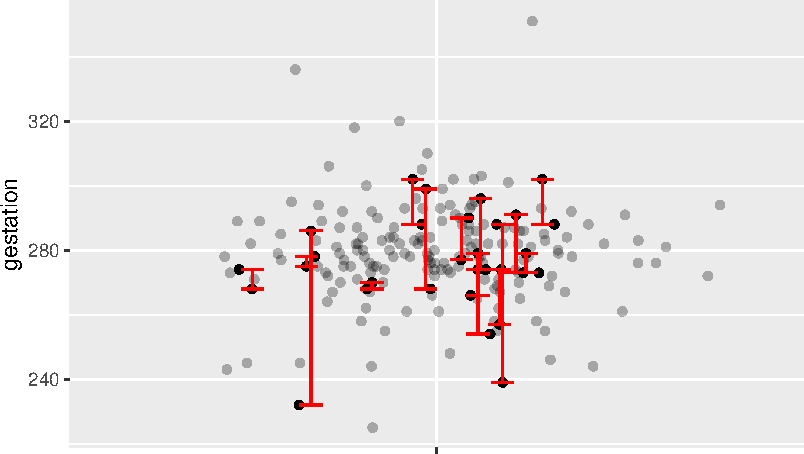
\includegraphics{test-tufte_files/figure-pdf/fig-explain-modulus-1.pdf}

}

\end{figure}%

Only a few pairs of points have been connected with the red lines. To
connect every possible pair of points would fill the graph with so many
lines that it would be impossible to see that each line connects a pair
of values.

The average square of the lines' lengths (in the vertical direction) is
called the ``modulus.'' We won't use this word going forward in these
Lessons; we accept that the conventional description of variation is the
``variance.'' Still, the modulus has a more natural explanation than the
variance. Numerically, the variance is half the modulus.

\end{tcolorbox}

Calculating the variance is straightforward using the \texttt{var()}
function. Remember, \texttt{var()} is similar to the other reduction
functions---e.g.~\texttt{mean()} and \texttt{median()}---that distill
multiple values into a single number. As always, the reduction functions
need to be used \emph{within} the arguments of a data wrangling
function.of a set of data-frame rows to a single summary is accomplished
with the \texttt{summarize()} wrangling command.

\begin{Shaded}
\begin{Highlighting}[]
\NormalTok{Gestation }\SpecialCharTok{|\textgreater{}}
  \FunctionTok{summarize}\NormalTok{(}\FunctionTok{var}\NormalTok{(gestation, }\AttributeTok{na.rm =} \ConstantTok{TRUE}\NormalTok{))}
\end{Highlighting}
\end{Shaded}

\begin{verbatim}


| var(gestation, na.rm = TRUE) |
|:----------------------------:|
|            256.9             |
\end{verbatim}

A consequence of the use of squaring in defining the variance is the
units of the result. \texttt{gestation} is measured in days, so
\texttt{var(gestation)} is measured in days-squared.

\begin{tcolorbox}[enhanced jigsaw, colbacktitle=quarto-callout-note-color!10!white, opacityback=0, breakable, opacitybacktitle=0.6, colback=white, coltitle=black, arc=.35mm, title=\textcolor{quarto-callout-note-color}{\faInfo}\hspace{0.5em}{From variance to ``standard deviation''}, left=2mm, colframe=quarto-callout-note-color-frame, rightrule=.15mm, bottomrule=.15mm, leftrule=.75mm, bottomtitle=1mm, toptitle=1mm, titlerule=0mm, toprule=.15mm]

If you have studied statistics before, you have probably encountered the
``\textbf{standard deviation}.'' We avoid this terminology; it is
long-winded and wrongly suggests a departure from the normal.
Calculating the standard deviation involves two steps: first, find the
variance then take the square root.

\begin{Shaded}
\begin{Highlighting}[]
\NormalTok{Gestation }\SpecialCharTok{|\textgreater{}}
  \FunctionTok{summarize}\NormalTok{(}\AttributeTok{sd =} \FunctionTok{sqrt}\NormalTok{(}\FunctionTok{var}\NormalTok{(gestation, }\AttributeTok{na.rm =} \ConstantTok{TRUE}\NormalTok{)) )}
\end{Highlighting}
\end{Shaded}

\end{tcolorbox}

\newpage

\section{Accounting for variation}\label{sec-accounting-for-variation}

Lesson \ref{sec-variation} listed three foundations for statistical
thinking and provided instruction on the first one:

\marginnote{\begin{footnotesize}

The word ``account'' has several related meanings. These definitions are
drawn from the Oxford Languages dictionaries.

\begin{itemize}
\tightlist
\item
  To ``account for something'' means ``to be the explanation or cause of
  something.'' {[}Oxford Languages{]}
\item
  An ``account of something'' is a story, a description, or an
  explanation, as in the Biblical account of the creation of the world.
\item
  To ``take account of something'' means ``to consider particular facts,
  circumstances, etc. when making a decision about something.''
\end{itemize}

Synonyms for ``account'' include ``description,''report,'' ``version,''
``story,'' ``statement,'' ``explanation,'' ``interpretation,''
``sketch,'' and ``portrayal.'' ``Accountants'' and their ``account
books'' keep track of where money comes from and goes to.

These various nuances of meaning, from a simple arithmetical tallying up
to an interpretative story serve the purposes of statistical thinking
well. When we ``account for variation,'' we are telling a story that
tries to explain where the variation might have come from. Although the
arithmetic used in the accounting is correct, the story behind the
accounting is not necessarily definitive, true, or helpful. Just as
witnesses of an event can have different accounts, so there can be many
accounts of the variation even of the same variable in the same data
frame.

\begin{center}\rule{0.5\linewidth}{0.5pt}\end{center}

\end{footnotesize}}

\begin{enumerate}
\def\labelenumi{\arabic{enumi}.}
\tightlist
\item
  How to measure the amount of variation
\end{enumerate}

In this Lesson, we will take on two and three:

\begin{enumerate}
\def\labelenumi{\arabic{enumi}.}
\setcounter{enumi}{1}
\tightlist
\item
  Accounting for variation
\item
  Measuring what remains unaccounted for
\end{enumerate}

In business, accounting keeps track of money and value: assets,
receipts, expenditures, etc. Likewise, in statistics, accounting for
variation is the process of keeping track of variation. At its most
basic, accounting for variation splits a variable into components: those
parts which can be attributed to one or more other variables and the
remainder which cannot be so attributed.

The variable being split up is called the ``\textbf{response
variable}.'' The human modeler chooses a response variable, depending on
her purpose for undertaking the work. The modeler also chooses
\emph{explanatory variables} that may account for some of the
variability in the response variable. There is almost always something
left over, variation that cannot be attributed to the explanatory
variables. This left-over part is called the ``\textbf{residual}.''

To illustrate, we'll return to a historical statistical landmark, the
data collected in the 1880s by Francis Galton on the heights of parents
and their full-grown children. In that era, there was much excitement,
uncertainty, and controversy about Charles Darwin's \emph{theory of
evolution}. {\marginnote{\begin{footnotesize}Remarkably, Galton was
Darwin's cousin.\end{footnotesize}}} Today, we understand the role of
DNA in encoding genetic information. But in Galton's day, the concept of
``gene'' was unknown.

\marginnote{\begin{footnotesize}

Each specimen is a full-grown child in the \texttt{Galton} data frame.
The variables recorded are the \texttt{height} of the child in inches,
the heights of the \texttt{mother} and \texttt{father}, and the
\texttt{sex} of the child according to the conventions of Victorian
England, where the data were collected.

\end{footnotesize}}

Galton's overall project was to quantify the heritability of traits
(such as height) from parents to offspring. Darwin had famously measured
the beaks of finches on the Galapagos Islands. Galton, in London, worked
with the most readily available local species: humans. Height is easy
and socially acceptable to measure, a good candidate for data
collection. {\marginnote{\begin{footnotesize}Galton \emph{invented} the
methods we are going to use in this example.\end{footnotesize}}}

Everyone can see that height varies from person to person. Galton sought
to divide the height variation in the children into two parts: that
which could be attributed to the parents and that which remained
unaccounted for, which we call the ``\textbf{residual}.'' We will start
with a mathematically more straightforward project: dividing the
variation in the children's heights into that part associated with the
child's sex and the residual.

As introduced in Lesson \ref{sec-wrangling}, we can calculate the
average height for females and males using the \texttt{summarize()}
wrangling verb with a \texttt{.by\ =\ sex} argument to create a separate
summary for each level of \texttt{sex}.

\begin{Shaded}
\begin{Highlighting}[]
\NormalTok{Galton }\SpecialCharTok{|\textgreater{}}
  \FunctionTok{summarize}\NormalTok{(}\AttributeTok{mheight =} \FunctionTok{mean}\NormalTok{(height), }\AttributeTok{.by =}\NormalTok{ sex)}
\end{Highlighting}
\end{Shaded}

{\marginnote{\begin{footnotesize}We often use \texttt{summarize()} with
reduction functions like \texttt{mean()}. Summarize gives one row of
output for each of the groups defined by the \texttt{.by\ =} argument.
Here we are using \texttt{mutate()}. The mean will still be calculated
on a group-by-group basis, but with \texttt{mutate()} the result will
contain all the original rows. Each row of a group will get the value
averaged over all the rows in that group.\end{footnotesize}}}

This simple report indicates that the sexes differ, on average, by about
5 inches in height. But this report offers no insight into how much of
the person-to-person variation in height is attributable to
\texttt{sex}. For that, we need to look at the group averages in the
context of the individuals. To that end, we will use \texttt{mutate()}
to assign to each individual a ``\textbf{model value}'' that depends
only on \texttt{sex}.

\begin{Shaded}
\begin{Highlighting}[]
\NormalTok{Model1 }\OtherTok{\textless{}{-}}\NormalTok{ Galton }\SpecialCharTok{|\textgreater{}}
  \FunctionTok{mutate}\NormalTok{(}\AttributeTok{modval =} \FunctionTok{mean}\NormalTok{(height), }\AttributeTok{.by =}\NormalTok{ sex) }
\end{Highlighting}
\end{Shaded}

Figure~\ref{fig-galton-model1b} shows \textbf{?@tbl-galton-model1c}
graphically. Some things to notice:

\begin{enumerate}
\def\labelenumi{\arabic{enumi}.}
\tightlist
\item
  The model values are different for males and females.
\item
  Among the females the model values do \emph{not} vary with
  \texttt{mother} or \texttt{father}. The same is true for the males.
\item
  The model values are not the same as the individual heights.
\end{enumerate}

\begin{figure}

\sidecaption{\label{fig-galton-model1b}The response variable
(\texttt{height}) and the model values from
\textbf{?@tbl-galton-model1c} plotted versus \texttt{sex}. The model
values are the same within each sex for all individuals.}

\centering{

\includegraphics{test-tufte_files/figure-pdf/fig-galton-model1b-1.pdf}

}

\end{figure}%

The numerical difference between each specimen's height and its model
value is called the ``\textbf{residual}'' for that specimen. This is
easy to calculate:

\begin{Shaded}
\begin{Highlighting}[]
\NormalTok{Model1 }\OtherTok{\textless{}{-}}\NormalTok{ Model1 }\SpecialCharTok{|\textgreater{}}
  \FunctionTok{mutate}\NormalTok{(}\AttributeTok{resid =}\NormalTok{ height }\SpecialCharTok{{-}}\NormalTok{ modval)}
\end{Highlighting}
\end{Shaded}

The residuals for the model of \texttt{height} versus \texttt{sex} are
shown in Table~\ref{tbl-galton-model1d}. Notice that some residuals are
positive, meaning that the actual \texttt{height} is larger than the
model value. Other residuals, when the actual \texttt{height} is below
the model value, are negative.

{\marginnote{\begin{footnotesize}\href{triangles}{Note to
instructors}\end{footnotesize}}}

As always, the variance is our preferred measure of the amount of
variation. There are three variances that are connected together:

\begin{enumerate}
\def\labelenumi{\roman{enumi}.}
\tightlist
\item
  The variance of the response variable.
\item
  The variance of the model values.
\item
  The variance (across all specimens) of the specimens' residuals.
\end{enumerate}

Comparing those three variances, we see that the largest one is the
variance of the response variable (\texttt{height}). This will always be
the case.

\begin{Shaded}
\begin{Highlighting}[]
\NormalTok{Model1 }\SpecialCharTok{|\textgreater{}}
  \FunctionTok{summarize}\NormalTok{(}\FunctionTok{var}\NormalTok{(height), }\FunctionTok{var}\NormalTok{(modval), }\FunctionTok{var}\NormalTok{(resid))}
\end{Highlighting}
\end{Shaded}

\begin{longtable}[]{@{}ccc@{}}
\toprule\noalign{}
var(height) & var(modval) & var(resid) \\
\midrule\noalign{}
\endhead
\bottomrule\noalign{}
\endlastfoot
12.84 & 6.549 & 6.288 \\
\end{longtable}

Remarkably, the variance of the model values and the variance of the
residuals add up precisely to equal the variance of the response
variable. In other words, the variation in the response variable is
split into two parts: the variation associated with the explanatory
variable and the remaining (``residual'') variation.

\subsection{Numerical explanatory
variables}\label{numerical-explanatory-variables}

The previous section used the categorical variable \texttt{sex} as the
explanatory variable. Galton's interest, however, was in the
relationship between children's and parents' height.

\texttt{sex} is a \emph{categorical} explanatory variable. Using
\texttt{mutate(...,\ .by\ =\ sex)} is a good method of handling
categorical explanatory variables. However, this does not work for
\emph{quantitative} explanatory variables. The reason is that
\texttt{.by} translates a quantitative variable into a categorical one,
with a result for each unique quantitative value: It's trivial to
substitute the height of the \texttt{mother} or \texttt{father} in place
of \texttt{sex} in the method introduced in the previous section.
However, as we shall see, the results are not satisfactory. Galton's key
discovery was the proper method for relating two \emph{quantitative}
variables such as \texttt{height} and \texttt{mother}.

First, let's try simply substituting in \texttt{mother} as the
explanatory variable and using \texttt{mean()} to create the model
values.

\begin{Shaded}
\begin{Highlighting}[]
\NormalTok{Model2 }\OtherTok{\textless{}{-}}\NormalTok{ Galton }\SpecialCharTok{|\textgreater{}}
  \FunctionTok{mutate}\NormalTok{(}\AttributeTok{modval =} \FunctionTok{mean}\NormalTok{(height),}
         \AttributeTok{resid =}\NormalTok{ height }\SpecialCharTok{{-}}\NormalTok{ modval,}
         \AttributeTok{.by =}\NormalTok{ mother) }
\NormalTok{Model2}
\end{Highlighting}
\end{Shaded}

\begin{longtable}[]{@{}cccc@{}}
\toprule\noalign{}
mother & sex & modval & resid \\
\midrule\noalign{}
\endhead
\bottomrule\noalign{}
\endlastfoot
58 & M & 67 & 5.4 \\
58 & F & 67 & -4.1 \\
58 & M & 67 & 1.4 \\
58 & M & 67 & 2.4 \\
64 & M & 66 & 2 \\
66 & M & 68 & 5.4 \\
67 & M & 67 & 6.3 \\
67 & F & 67 & 2.1 \\
\end{longtable}

The problem is that the model values are not a simple function of
\texttt{mother}, as seen in Figure~\ref{fig-group-by-mother}.

\begin{Shaded}
\begin{Highlighting}[]
\NormalTok{Model2 }\SpecialCharTok{|\textgreater{}} 
  \FunctionTok{gf\_point}\NormalTok{(height }\SpecialCharTok{\textasciitilde{}}\NormalTok{ mother, }\AttributeTok{point\_ink =} \FloatTok{0.1}\NormalTok{) }\SpecialCharTok{|\textgreater{}} 
  \FunctionTok{gf\_point}\NormalTok{(modval }\SpecialCharTok{\textasciitilde{}}\NormalTok{ mother, }\AttributeTok{color=}\StringTok{"blue"}\NormalTok{, }\AttributeTok{point\_ink =} \FloatTok{0.3}\NormalTok{) }\SpecialCharTok{|\textgreater{}}
  \FunctionTok{gf\_line}\NormalTok{(modval }\SpecialCharTok{\textasciitilde{}}\NormalTok{ mother, }\AttributeTok{color=}\StringTok{"blue"}\NormalTok{, }\AttributeTok{linewidth=}\FloatTok{0.5}\NormalTok{, }\AttributeTok{alpha =} \FloatTok{0.5}\NormalTok{ ) }\SpecialCharTok{|\textgreater{}}
  \FunctionTok{gf\_rect}\NormalTok{(}\DecValTok{62} \SpecialCharTok{+} \DecValTok{73} \SpecialCharTok{\textasciitilde{}} \FloatTok{60.25} \SpecialCharTok{+} \FloatTok{61.75}\NormalTok{, }\AttributeTok{fill=}\ConstantTok{NA}\NormalTok{, }\AttributeTok{color =} \StringTok{"orange"}\NormalTok{)}
\end{Highlighting}
\end{Shaded}

\begin{figure}[H]

\centering{

\includegraphics{test-tufte_files/figure-pdf/fig-group-by-mother-1.pdf}

}

\caption{\label{fig-group-by-mother}Modeling \texttt{height} of the
child by the \texttt{mother}'s height using \texttt{group\_by(mother)}
and \texttt{modval=mean(height)}. It's hard to see any pattern in the
model values. A thin line has been added connecting adjacent model
values to highlight how unsatisfactory the model is.}

\end{figure}%

It is common sense that the model linking mothers' heights to children's
height should be \textbf{smooth}, not the jagged pattern seen in
Figure~\ref{fig-group-by-mother}. The source of the jaggedness is the
use of \texttt{.by\ =\ mother} in
\texttt{mutate(modval\ =\ mean(height),\ .by\ =\ mother)}. The
calculation of the mean is done separately and independently for each of
the vertical columns of points in Figure~\ref{fig-group-by-mother}. To
illustrate, compare the model values for 60.5-inch mothers, 61-inch
mothers, and 61.5-inch mothers (highlighted by the orange box). In a
smooth relationship, for example, the model value for 61.0-inch mothers
should be about halfway between the model values for 60.5- and 61.5-inch
mothers. Instead, the \texttt{.by=mother} model produces a model value
for 61.0-inch mothers that is lower than the model values on either side
of it. In a smooth model, the model value for mothers of middle height
should be somewhere in between the model values for short and for tall
mothers.

The solution to the problem of jagged model values is to avoid the
absolute splitting into non-overlapping groups by mother's height.
Instead, we want to find a smooth relationship. Galton invented the
method for accomplishing this. A modern form of his method is provided
by the \texttt{model\_values()} function, which we shall use to
construct \texttt{Model3}.

\begin{Shaded}
\begin{Highlighting}[]
\NormalTok{Model3 }\OtherTok{\textless{}{-}}\NormalTok{ Galton }\SpecialCharTok{|\textgreater{}}
  \FunctionTok{mutate}\NormalTok{(}\AttributeTok{modval =} \FunctionTok{model\_values}\NormalTok{(height }\SpecialCharTok{\textasciitilde{}}\NormalTok{ mother),}
         \AttributeTok{resid =}\NormalTok{ height }\SpecialCharTok{{-}}\NormalTok{ modval)}
\end{Highlighting}
\end{Shaded}

Notice that the \texttt{.by\ =\ mother} step has been entirely removed.
Notice also that \texttt{model\_values()} uses the same kind of
\textbf{tilde expression} as we have employed when plotting. The
response variable is listed on the left of the
\includegraphics{www/tilde.png}, the explanatory variable on the right
side. In other words, we are modeling the child's \texttt{height} as a
function of \texttt{mother}'s height.

\begin{Shaded}
\begin{Highlighting}[]
\NormalTok{Model3 }\SpecialCharTok{|\textgreater{}} 
  \FunctionTok{gf\_point}\NormalTok{(height }\SpecialCharTok{\textasciitilde{}}\NormalTok{ mother, }\AttributeTok{point\_ink =} \FloatTok{0.1}\NormalTok{) }\SpecialCharTok{|\textgreater{}} 
  \FunctionTok{gf\_point}\NormalTok{(modval }\SpecialCharTok{\textasciitilde{}}\NormalTok{ mother, }\AttributeTok{color=}\StringTok{"blue"}\NormalTok{, }\AttributeTok{point\_ink =} \FloatTok{0.3}\NormalTok{) }\SpecialCharTok{|\textgreater{}}
  \FunctionTok{gf\_line}\NormalTok{(modval }\SpecialCharTok{\textasciitilde{}}\NormalTok{ mother, }\AttributeTok{color=}\StringTok{"blue"}\NormalTok{, }\AttributeTok{linewidth=}\FloatTok{0.5}\NormalTok{) }\SpecialCharTok{|\textgreater{}}
  \FunctionTok{gf\_rect}\NormalTok{(}\DecValTok{62} \SpecialCharTok{+} \DecValTok{73} \SpecialCharTok{\textasciitilde{}} \FloatTok{60.25} \SpecialCharTok{+} \FloatTok{61.75}\NormalTok{, }\AttributeTok{fill=}\ConstantTok{NA}\NormalTok{, }\AttributeTok{color =} \StringTok{"orange"}\NormalTok{)}
\end{Highlighting}
\end{Shaded}

\begin{figure}[H]

\centering{

\includegraphics{test-tufte_files/figure-pdf/fig-model3-1.pdf}

}

\caption{\label{fig-model3}A smooth model of \texttt{height} with
respect to \texttt{mother} created with
\texttt{model\_values(height\ \textasciitilde{}\ sex)}.}

\end{figure}%

As always, modeling splits the variance of the response variable into
two parts, one associated with the explanatory variable and the other
holding what's left over: the residual. Here's the split for
\texttt{Model3} which uses \texttt{mother} as an explanatory variable:

\begin{Shaded}
\begin{Highlighting}[]
\NormalTok{Model3 }\SpecialCharTok{|\textgreater{}}
  \FunctionTok{summarize}\NormalTok{(}\FunctionTok{var}\NormalTok{(height), }\FunctionTok{var}\NormalTok{(modval), }\FunctionTok{var}\NormalTok{(resid))}
\end{Highlighting}
\end{Shaded}

\begin{longtable}[]{@{}ccc@{}}
\toprule\noalign{}
var(height) & var(modval) & var(resid) \\
\midrule\noalign{}
\endhead
\bottomrule\noalign{}
\endlastfoot
12.84 & 0.52 & 12.32 \\
\end{longtable}

\subsection{Multiple explanatory variables}\label{sec-multiple-vars1}

The models we work with in these Lessons \emph{always} have exactly one
response variable. {\marginnote{\begin{footnotesize}Note that the idea
of ``response'' and ``explanatory'' variables refers to a model and are
not at all intrinsic to a bare data frame. A data frame can contain many
variables, any of which can be used as explanatory variables. The choice
of response variable depends on the modeler's goals.\end{footnotesize}}}
But models can have any number of \emph{explanatory} variables.

Whatever the number of explanatory variables and however many levels a
categorical explanatory variable has the model splits the variance of
the response into two complementary pieces: the variance accounted for
by the explanatory variables and the part not accounted for, that is,
the \emph{residual} variance. {\marginnote{\begin{footnotesize}Many
statistical terms mean something different in statistical than in
everyday use. ``Residual'' is a pleasant exception: the statistical
meaning is closely matched by its everyday dictionary
definition.\end{footnotesize}}} To illustrate, here is a sequence of
models of \texttt{height} with different numbers of explanatory
variables.

\textbf{Three explanatory variables}

\begin{Shaded}
\begin{Highlighting}[]
\DocumentationTok{\#\#\# | column: margin}
\NormalTok{Galton }\SpecialCharTok{|\textgreater{}}
  \FunctionTok{mutate}\NormalTok{(}\AttributeTok{modval =} \FunctionTok{model\_values}\NormalTok{(height }\SpecialCharTok{\textasciitilde{}}\NormalTok{ sex }\SpecialCharTok{+}\NormalTok{ mother }\SpecialCharTok{+}\NormalTok{ father),}
         \AttributeTok{resid =}\NormalTok{ height }\SpecialCharTok{{-}}\NormalTok{ modval) }\SpecialCharTok{|\textgreater{}}
  \FunctionTok{summarize}\NormalTok{(}\FunctionTok{var}\NormalTok{(height), }\FunctionTok{var}\NormalTok{(modval), }\FunctionTok{var}\NormalTok{(resid))}
\end{Highlighting}
\end{Shaded}

\begin{longtable}[]{@{}ccc@{}}
\toprule\noalign{}
var(height) & var(modval) & var(resid) \\
\midrule\noalign{}
\endhead
\bottomrule\noalign{}
\endlastfoot
12.84 & 8.212 & 4.626 \\
\end{longtable}

\textbf{Two explanatory variables}

\begin{Shaded}
\begin{Highlighting}[]
\DocumentationTok{\#\#\#| column: margin}
\NormalTok{Galton }\SpecialCharTok{|\textgreater{}}
  \FunctionTok{mutate}\NormalTok{(}\AttributeTok{modval =} \FunctionTok{model\_values}\NormalTok{(height }\SpecialCharTok{\textasciitilde{}}\NormalTok{ sex }\SpecialCharTok{+}\NormalTok{ mother),}
         \AttributeTok{resid =}\NormalTok{ height }\SpecialCharTok{{-}}\NormalTok{ modval) }\SpecialCharTok{|\textgreater{}}
  \FunctionTok{summarize}\NormalTok{(}\FunctionTok{var}\NormalTok{(height), }\FunctionTok{var}\NormalTok{(modval), }\FunctionTok{var}\NormalTok{(resid))}
\end{Highlighting}
\end{Shaded}

\begin{longtable}[]{@{}ccc@{}}
\toprule\noalign{}
var(height) & var(modval) & var(resid) \\
\midrule\noalign{}
\endhead
\bottomrule\noalign{}
\endlastfoot
12.84 & 7.212 & 5.625 \\
\end{longtable}

\textbf{One explanatory variable}

\begin{Shaded}
\begin{Highlighting}[]
\DocumentationTok{\#\#\# | column: margin}
\NormalTok{Galton }\SpecialCharTok{|\textgreater{}}
  \FunctionTok{mutate}\NormalTok{(}\AttributeTok{modval =} \FunctionTok{model\_values}\NormalTok{(height }\SpecialCharTok{\textasciitilde{}}\NormalTok{ sex),}
         \AttributeTok{resid =}\NormalTok{ height }\SpecialCharTok{{-}}\NormalTok{ modval) }\SpecialCharTok{|\textgreater{}}
  \FunctionTok{summarize}\NormalTok{(}\FunctionTok{var}\NormalTok{(height), }\FunctionTok{var}\NormalTok{(modval), }\FunctionTok{var}\NormalTok{(resid))}
\end{Highlighting}
\end{Shaded}

\begin{longtable}[]{@{}ccc@{}}
\toprule\noalign{}
var(height) & var(modval) & var(resid) \\
\midrule\noalign{}
\endhead
\bottomrule\noalign{}
\endlastfoot
12.84 & 6.549 & 6.288 \\
\end{longtable}

\textbf{Zero explanatory variables}

\begin{Shaded}
\begin{Highlighting}[]
\DocumentationTok{\#\#\# | column: margin}
\CommentTok{\# Galton |\textgreater{}}
\CommentTok{\#   mutate(modval = model\_values(height \textasciitilde{} 1),}
\CommentTok{\#          resid = height {-} modval) |\textgreater{}}
\CommentTok{\#   summarize(var(height), var(modval), var(resid))}
\end{Highlighting}
\end{Shaded}

\begin{longtable}[]{@{}ccc@{}}
\toprule\noalign{}
var(height) & var(modval) & var(resid) \\
\midrule\noalign{}
\endhead
\bottomrule\noalign{}
\endlastfoot
12.84 & 0 & 12.84 \\
\end{longtable}

\subsection{\texorpdfstring{Comparing models with
R\textsuperscript{2}}{Comparing models with R2}}\label{comparing-models-with-r2}

When selecting explanatory variables, comparing two or more different
models sharing the same response variable is often helpful: a simple
model and a model that adds one or more explanatory variables to the
simple model. The model with \emph{no explanatory variables}, is always
the simplest possible model. For example, in
Section~\ref{sec-multiple-vars1}, the model
\texttt{height\ \textasciitilde{}\ 1} is the simplest. Compared to the
simplest model, the model \texttt{height\ \textasciitilde{}\ sex} has
one additional explanatory variable, \texttt{sex}. Similarly,
\texttt{height\ \textasciitilde{}\ sex\ +\ mother} has one additional
explanatory variable compared to
\texttt{height\ \textasciitilde{}\ sex}, and
\texttt{height\ \textasciitilde{}\ sex\ +\ mother\ +\ father} adds in
still another explanatory variable.

The simpler model is said to be ``\textbf{nested in}'' the more
extensive model, analogous to a series of
\href{https://en.wikipedia.org/wiki/Matryoshka_doll}{Matroshka dolls}. A
simple measure of how much of the response variance is accounted for by
the explanatory variables is the ratio of the variance of the model
values divided by the variance of the response variable itself. This
ratio is called ``R\textsuperscript{2}'', pronounced ``R-squared.''

\marginnote{\begin{footnotesize}

\includegraphics{www/Russian-Matroshka_no_bg.jpeg}

A sequence of five nested Matroshka dolls. Each smaller doll fits inside
a larger one.

\end{footnotesize}}

For instance, R\^{}2 for the model
\texttt{height\ \textasciitilde{}\ sex\ +\ mother} is
\[\text{R}^2 = \frac{7.21}{12.84} = 0.56\]
{\marginnote{\begin{footnotesize}R\textsuperscript{2} is also known as
the ``coefficient of determination,'' a little-used term we shall avoid.
Still, it's worth noting the attitude behind the term; it quantifies the
extent to which the response variable is ``determined'' by the
explanatory variables.\end{footnotesize}}} By comparison, R\^{}2 for the
simpler model, \texttt{height\ \textasciitilde{}\ sex,} is slightly
smaller:

\[\text{R}^2 = \frac{6.55}{12.84} = 0.51\] For all models, \(0 \leq\)
R\textsuperscript{2} \(\leq 1\).
{\marginnote{\begin{footnotesize}Instructor Note: Strictly speaking,
``all'' should be qualified to mean ``linear least-squares models with
an intercept term.''\end{footnotesize}}} It is tempting to believe that
the ``best'' model in a set of nested models is the one with the highest
R\textsuperscript{2}, but statistical thinkers understand that ``best''
ought to depend on the purpose for which the model is being built. This
matter will be a major theme in the remaining Lessons.

\newpage

\section{Model patterns}\label{sec-model-patterns}

In these Lessons, we build many models using many different data
sources. Notably, we often build multiple models from one data frame.
These models use the \emph{same response variable} but different
explanatory variables. This enables us to compare different ways of
explaining the variation in the response variable.

All of the models will have certain features in common. This Lesson
points out those commonalities so that you can ``read'' a new model with
understanding.

\subsection{Data and patterns: a painterly
metaphor}\label{data-and-patterns-a-painterly-metaphor}

Figure~\ref{fig-signac-full} is a painting of a harbor scene in
Istambul. It's a rich composition intended for the human eye. There is
water, a dozen boats, and a mosque---the Hagia Sophia---in the
background.

\begin{figure}

\centering{

\includegraphics{www/Signac-full-small.jpeg}

}

\caption{\label{fig-signac-full}Paul Signac,
\href{https://en.m.wikipedia.org/wiki/File:Signac_Paul_-_La_Corne_d\%27Or.jpg}{\emph{La
Corne d'Or}}, 1907}

\end{figure}%

It's tempting to hope that statistical techniques could identify complex
patterns like those we see in Figure~\ref{fig-signac-full}. That task
might barely be possible by the most up-to-date forms of artificial
intelligence. Statistical modeling, however, is intended to look for
much simpler patterns.

To emphasize just how simple such patterns are,
\textbf{?@fig-paint-strokes} zooms in on a tiny area of the paining,
containing just a handful of paint strokes.

It goes without saying that those few strokes give no hint about what is
going on in the whole painting. We don't expect them to.

Statistical modeling looks only for very general kinds of patterns. Not
a harbor, not a boat, not even a mast or pennant. Much simpler, and much
more general.

\textbf{?@fig-paint-edge}, which shows a much larger part of the
painting than \textbf{?@fig-paint-strokes}, illustrates one kind of
simple, general pattern: a boundary or ``edge.'' The edge here is
between the bright zone on the lower left and the darker zone on the top
right. A statistical model would be able to confirm that there is such
an edge and give a little more detail: the orientation of the edge and
which side is bright and which side dark.

There is nothing in \textbf{?@fig-paint-edge} to discern that the edge
in question is between the reflection of the sky and the prow of a boat.
It's just an abstract edge.

This Lesson describes how we specify to the computer the kind of simple,
general pattern we are looking for in data. It also shows the ``shapes''
of those patterns not as painting-like image but as a model annotation
in a point plot.

\subsection{The model specification}\label{the-model-specification}

Two basic inputs go into constructing a model:

\begin{enumerate}
\def\labelenumi{\arabic{enumi}.}
\tightlist
\item
  A data frame.
\item
  The \textbf{model specification}, which declares which column from the
  data frame will be the response variable and which other column(s)
  will be the explanatory variable(s).
\end{enumerate}

For directing the computer, we write the model specification as a
\textbf{tilde expression}: the name of the response variable goes to the
left of the \includegraphics{www/tilde.png}. The name of the explanatory
variable is on the right.

When there is more than one explanatory variable, their names all go on
the right side of \includegraphics{www/tilde.png} separated by the
\texttt{+} symbol which stands for the English word ``and'' rather than
an sum in the arithmetic sense.
{\marginnote{\begin{footnotesize}Occasionally, we will use the
\texttt{*} symbol instead of \texttt{+} for reasons that will be pointed
out whenever we come to such a situation. We will also sometimes use
mathematical functions such as \texttt{log()} or \texttt{ns()} in the
model specification.\end{footnotesize}}}

From time to time, we refer to models with \emph{no explanatory
variables}. In such models, a simple \texttt{1} goes to the right of the
\includegraphics{www/tilde.png}. The reasons for doing this require some
explanation, which will be provided in later Lessons.

\subsection{``Shapes'' of models}\label{shapes-of-models}

Although the response variable in a regression model is always
quantitative, explanatory variables can be either quantitative or
categorical. Regression models may sometimes involve tens or thousands
of explanatory variables in professional work. Almost all the models
used in these Lessons will have one or two explanatory variables (and,
occasionally, zero explanatory variables). This suffices for introducing
the concepts and methods of statistical thinking.

It is convenient to think of the various combinations of explanatory
variables in terms of the ``shape'' of a graph of the model. There are
two basic shapes for models with a single explanatory variable: one
shape when the explanatory variable is \emph{categorical} and another
shape when the explanatory variable is quantitative.

We illustrate with the \texttt{CPS85} data frame. \texttt{CPS85} records
a small survey of workers' \texttt{wage}s (in 1985) and includes both
numerical and categorical variables. The unit of observation is an
individual worker. The categorical variable \texttt{sector} records the
type of each worker's job; levels for \texttt{sector} include clerical,
manufacturing, sales, service. etc.

In the following subsections, we compare the shapes of several models,
all of which use \texttt{wage} as the response variable.

\subsubsection{One explanatory variable}\label{one-explanatory-variable}

First, consider models with a single explanatory variable. When that
explanatory variable is categorical, the model shape consists of
potentially different values for each level of the explanatory variable.
Figure~\ref{fig-single-categorical} shows two examples:

\begin{figure*}

\centering{

\begin{figure}[H]

\begin{minipage}{0.33\linewidth}

\includegraphics{test-tufte_files/figure-pdf/unnamed-chunk-121-1.pdf}

\subcaption{\label{}\texttt{wage\ \textasciitilde{}\ union}}
\end{minipage}%
%
\begin{minipage}{0.33\linewidth}

\includegraphics{test-tufte_files/figure-pdf/unnamed-chunk-121-2.pdf}

\subcaption{\label{}\texttt{wage\ \textasciitilde{}\ sector}}
\end{minipage}%
%
\begin{minipage}{0.33\linewidth}

\includegraphics{test-tufte_files/figure-pdf/unnamed-chunk-121-3.pdf}

\subcaption{\label{}\texttt{wage\ \textasciitilde{}\ married}}
\end{minipage}%

\end{figure}%

}

\caption{\label{fig-single-categorical}Examples of regression models
with a single categorical explanatory variable.}

\end{figure*}%

When the explanatory variable is quantitative, the model values are
arrayed on a smooth curve, as in Figure~\ref{fig-single-quant}.

\begin{figure*}

\centering{

\begin{figure}[H]

\begin{minipage}{0.33\linewidth}

\includegraphics{test-tufte_files/figure-pdf/unnamed-chunk-122-1.pdf}

\subcaption{\label{}\texttt{wage\ \textasciitilde{}\ exper}}
\end{minipage}%
%
\begin{minipage}{0.33\linewidth}

\includegraphics{test-tufte_files/figure-pdf/unnamed-chunk-122-2.pdf}

\subcaption{\label{}\texttt{wage\ \textasciitilde{}\ educ}}
\end{minipage}%
%
\begin{minipage}{0.33\linewidth}

\includegraphics{test-tufte_files/figure-pdf/unnamed-chunk-122-3.pdf}

\subcaption{\label{}\texttt{wage\ \textasciitilde{}\ ns(age,\ 3)}}
\end{minipage}%

\end{figure}%

}

\caption{\label{fig-single-quant}Examples of regression models with a
single quantitative explanatory variable.}

\end{figure*}%

\subsubsection{Two explanatory
variables}\label{sec-two-explanatory-variables}

Explanatory variables can be either quantitative or categorical. With
two explanatory variables, one is mapped to x and the other to color.
Given that the response variable is always mapped to y, there are four
combinations possible, each of which has a distinctive graphical format:

\begin{longtable}[]{@{}lll@{}}
\toprule\noalign{}
Example & Horizontal axis (x) & Color \\
\midrule\noalign{}
\endhead
\bottomrule\noalign{}
\endlastfoot
Figure~\ref{fig-cat-cat} & categorical & categorical \\
Figure~\ref{fig-cat-quant} & categorical & quantitative \\
Figure~\ref{fig-quant-cat} & quantitative & categorical \\
Figure~\ref{fig-quant-quant} & quantitative & quantitative \\
\end{longtable}

\textbf{Two categorical explanatory variables}

\begin{figure}

\centering{

\begin{Shaded}
\begin{Highlighting}[]
\NormalTok{Whickham }\SpecialCharTok{|\textgreater{}} 
  \FunctionTok{point\_plot}\NormalTok{(age    }\SpecialCharTok{\textasciitilde{}}\NormalTok{ smoker }\SpecialCharTok{+}\NormalTok{ outcome, }\AttributeTok{annot=}\StringTok{"model"}\NormalTok{, }
             \AttributeTok{point\_ink =} \FloatTok{0.05}\NormalTok{, }\AttributeTok{model\_ink=}\FloatTok{0.7}\NormalTok{) }
\end{Highlighting}
\end{Shaded}

\includegraphics{test-tufte_files/figure-pdf/unnamed-chunk-123-1.pdf}

}

\caption{\label{fig-cat-cat}\texttt{age\ \textasciitilde{}\ smoker\ +\ outcome}}

\end{figure}%

This example shows data from a survey of female voters in the UK. Each
voter's age and smoking status were recorded at an initial interview.
The interview was followed up 20 years later, at which point some of the
original interviewees were dead and others still living, recorded in the
variable \texttt{outcome}. Unsurprisingly, the older interviewees were
much more likely to have died during the 20-year follow-up. The model
values show the difference in mean ages between the smokers and
non-smokers separately for the survivors and non-survivors. With two
categorical variables, each with two levels, there are four distinct
model values.

\textbf{Categorical \& quantitative}

This example shows (full-grown) child's height as a function of the
child's sex and his or her mother's height.

\begin{Shaded}
\begin{Highlighting}[]
\CommentTok{\# The code version to appear in the text}
\NormalTok{Galton }\SpecialCharTok{|\textgreater{}} 
  \FunctionTok{point\_plot}\NormalTok{(height }\SpecialCharTok{\textasciitilde{}}\NormalTok{ sex }\SpecialCharTok{+}\NormalTok{ mother, }\AttributeTok{point\_ink =} \FloatTok{0.2}\NormalTok{)}
\NormalTok{Galton }\SpecialCharTok{|\textgreater{}} 
  \FunctionTok{mutate}\NormalTok{(}\AttributeTok{modval =} \FunctionTok{model\_values}\NormalTok{(height }\SpecialCharTok{\textasciitilde{}}\NormalTok{ sex }\SpecialCharTok{+}\NormalTok{ mother)) }\SpecialCharTok{|\textgreater{}}
  \FunctionTok{point\_plot}\NormalTok{(modval }\SpecialCharTok{\textasciitilde{}}\NormalTok{ sex }\SpecialCharTok{+}\NormalTok{ mother) }\SpecialCharTok{|\textgreater{}}
  \FunctionTok{gf\_lims}\NormalTok{(}\AttributeTok{y =} \FunctionTok{c}\NormalTok{(}\DecValTok{55}\NormalTok{, }\DecValTok{80}\NormalTok{))}
\end{Highlighting}
\end{Shaded}

\begin{figure}

\centering{

\begin{figure}[H]

{\centering \includegraphics{test-tufte_files/figure-pdf/unnamed-chunk-125-1.pdf}

}

\caption{Data layer}

\end{figure}%

\begin{figure}[H]

{\centering \includegraphics{test-tufte_files/figure-pdf/unnamed-chunk-125-2.pdf}

}

\caption{Model-value layer}

\end{figure}%

}

\caption{\label{fig-cat-quant}\texttt{height\ \textasciitilde{}\ sex\ +\ mother}}

\end{figure}%

Reading such a graph takes patience. We've tried to help by separating
the data and model-value layers. In the data layer, you can easily see
that some males are taller than almost all females, and some females are
shorter than nearly all males. The model layer strips away the
residuals, producing a discernible pattern: the shorter children of
either sex tend to have shorter mothers (black) and that taller children
of each sex tend to have taller mothers (orange).

The model-value layer shows the extent of the relationship between
mother's and child's height more clearly. (This is exactly what models
are supposed to do!) You can see that the model values differ for
children of the shortest mothers and of the tallest mothers. The
different is about 3 inches of child's height.

The model values are faithful to the data, but leave out the residuals.
The raw data include the residuals. The non-zero size of residuals means
that children of the shortest mothers differ in height from the model
values. Similarly for the children of the tallest mothers. The result
is, in the raw data, that some children of the shorter mothers are in
fact taller than some children of the taller mothers. The model values,
by stripping away the residual child-to-child differences, make the
trends easier to see.

\textbf{Quantitative \& categorical}

This example shows the same data and model as the previous example. The
only difference is that the quantitative explanatory variable is mapped
to x while the categorical explanatory variable is mapped to color.

Point for point, the model values in Figure~\ref{fig-quant-cat} are the
same as in Figure~\ref{fig-cat-quant}. But the new arrangement spreads
them out differently in space. In Figure~\ref{fig-quant-cat} the model
values are organized along two straight lines, one for each sex. The
\textbf{slope} of the lines indicates the relationship between mother's
and child's heights. The vertical offset between the lines is the
difference in model values for the two sexes.

Figure~\ref{fig-quant-cat} is easier to read than
Figure~\ref{fig-cat-quant}. This illustrates a simple principle for
effective graphics: When a model has one quantitative and one
categorical explanatory variable, map the quantitative variable to the
horizontal axis.

\begin{Shaded}
\begin{Highlighting}[]
\NormalTok{Galton }\SpecialCharTok{|\textgreater{}} 
  \FunctionTok{point\_plot}\NormalTok{(height }\SpecialCharTok{\textasciitilde{}}\NormalTok{ mother }\SpecialCharTok{+}\NormalTok{ sex, }\AttributeTok{annot=}\StringTok{"model"}\NormalTok{, }
             \AttributeTok{point\_ink =} \FloatTok{0.1}\NormalTok{, }\AttributeTok{model\_ink=}\FloatTok{0.7}\NormalTok{)}
\end{Highlighting}
\end{Shaded}

\begin{figure}[H]

\centering{

\includegraphics{test-tufte_files/figure-pdf/fig-quant-cat-1.pdf}

}

\caption{\label{fig-quant-cat}Mapping the quantitative explanatory
variable to the horizontal axis.}

\end{figure}%

\textbf{Two quantitative explanatory variables}

This example draws on the same data frame as the previous two examples,
but we use the mother's and father's heights for the explanatory
variables. Both these explanatory variables are quantitative.

\begin{Shaded}
\begin{Highlighting}[]
\NormalTok{Galton }\SpecialCharTok{|\textgreater{}} \FunctionTok{point\_plot}\NormalTok{(height }\SpecialCharTok{\textasciitilde{}}\NormalTok{ mother }\SpecialCharTok{+}\NormalTok{ father) }
\NormalTok{Galton }\SpecialCharTok{|\textgreater{}} 
  \FunctionTok{mutate}\NormalTok{(}\AttributeTok{modvals =} 
           \FunctionTok{model\_values}\NormalTok{(height }\SpecialCharTok{\textasciitilde{}}\NormalTok{ mother }\SpecialCharTok{+}\NormalTok{ father)) }\SpecialCharTok{|\textgreater{}}
  \FunctionTok{point\_plot}\NormalTok{(modvals }\SpecialCharTok{\textasciitilde{}}\NormalTok{ mother }\SpecialCharTok{+}\NormalTok{ father) }\SpecialCharTok{|\textgreater{}} 
  \FunctionTok{gf\_lims}\NormalTok{(}\AttributeTok{y=}\FunctionTok{c}\NormalTok{(}\DecValTok{55}\NormalTok{,}\DecValTok{80}\NormalTok{))}
\end{Highlighting}
\end{Shaded}

\begin{figure}[H]

\centering{

\centering{

\includegraphics{test-tufte_files/figure-pdf/fig-quant-quant-1.pdf}

}

\subcaption{\label{fig-quant-quant-1}Data layer}

\centering{

\includegraphics{test-tufte_files/figure-pdf/fig-quant-quant-2.pdf}

}

\subcaption{\label{fig-quant-quant-2}Model-value layer}

}

\caption{\label{fig-quant-quant}\texttt{height\ \textasciitilde{}\ mother\ +\ father}}

\end{figure}%

As in Figure~\ref{fig-cat-quant}, mapping a \emph{quantitative} variable
to color makes the graph hard to read. To simplify, we've separated the
data layer from the model layer.

It's almost impossible to see the relationship between fathers and
children's heights in the data layer. By stripping away the
child-to-child residuals, the model-value layer clarifies the pattern.
\texttt{father} is mapped to color, so the color strata represents the
father/child relationship: shorter fathers (black) are tend to be lower
on the y scale that represents the child's height. Taller fathers
(orange) are associated with higher y values, that is, taller children.
\texttt{mother} is mapped to x, so the mother/child relationship appears
in the upward slope of the cloud of model-values, similar to the slope
in Figure~\ref{fig-quant-cat}.

\newpage

\section{Model functions}\label{sec-regression}

From the start of these Lessons, we have talked about revealing patterns
in data, particularly those that describe relationships among variables.
Graphics show patterns in a way that is particularly attuned to human
cognition, and we have leaned on them heavily. In this Lesson, we turn
to another form of description of relationships between variables:
simple mathematical functions.

\subsection{Basics of mathematical
functions}\label{sec-math-function-basics}

We will need only the most basic ideas of mathematics to enable our work
with functions. There won't be any algebra required.

\begin{enumerate}
\def\labelenumi{\arabic{enumi}.}
\item
  In mathematics, a function is a relationship between one or more
  inputs and an output. In our use of functions for statistical
  thinking, the output corresponds to the response variable, the inputs
  to the explanatory variables.
\item
  In mathematical notation, functions are conventionally written
  idiomatically using single-letter names. For instance, letters from
  the end of the alphabet---\(x\), \(y\), \(t\), and \(z\)---are names
  for function inputs. The convention uses letters from the start of the
  alphabet as stand-ins for numerical values; these are called
  \textbf{parameters} or, equivalently, \textbf{coefficients}. These
  conventions are almost 400 years old and are associated with Isaac
  Newton (1643-1727).

  Not quite 300 years ago, a new mathematical idea, the function, was
  introduced by Leonhard Euler (1707-1783). Since the start and end of
  the alphabet had been reserved for names of variables and parameters,
  a convention emerged to use the letters \(f\) and \(g\) for function
  names.
\item
  To say, ``Use function \(f\) to transform the inputs \(x\) and \(t\)
  to an output value,'' the notation is \(f(x, t)\). To emphasize:
  Remember that \(f(x, t)\) stands for the \textbf{output} of the
  function. Statistics often uses the one-letter name style, but when
  the letters stand for things in the real world, it can be preferable
  to use names that remind us what they stand for: \texttt{age},
  \texttt{time\_of\_day}, \texttt{mother}, \texttt{wrist},
  \texttt{prices}, and such.
\item
  Mathematical functions are idealizations. Importantly, they differ
  from much of everyday experience. Every mathematical function may have
  only one \emph{output value} for any given \emph{input value}. We say
  that mathematical functions are ``\textbf{single valued}. For
  instance, the mathematical value \(f(x=3, t=10)\) will be the same
  every time it is calculated. In everyday life, a quantity like
  \texttt{cooking\_time(temperature=300)}might vary depending on other
  factors (like \texttt{altitude}) or even randomly.

  When functions are graphed, the single-valued property is shown using
  a thin line for the function value, as it depends on the inputs. (See
  Figure~\ref{fig-single-valued}.)
\end{enumerate}

\begin{marginfigure}

\centering{

\begin{figure}[H]

\begin{minipage}{\linewidth}

\includegraphics{test-tufte_files/figure-pdf/unnamed-chunk-130-1.pdf}

\subcaption{\label{}Straight-line function}
\end{minipage}%
\newline
\begin{minipage}{\linewidth}

\includegraphics{test-tufte_files/figure-pdf/unnamed-chunk-130-2.pdf}

\subcaption{\label{}Sigmoidal function}
\end{minipage}%
\newline
\begin{minipage}{\linewidth}

\includegraphics{test-tufte_files/figure-pdf/unnamed-chunk-130-3.pdf}

\subcaption{\label{}Discrete-input function}
\end{minipage}%

\end{figure}%

}

\caption{\label{fig-single-valued}Three examples of single-valued
functions.}

\end{marginfigure}%

\begin{enumerate}
\def\labelenumi{\arabic{enumi}.}
\setcounter{enumi}{4}
\tightlist
\item
  In contrast to the large variety encountered in mathematics courses,
  we will need only the three function types shown in
  Figure~\ref{fig-single-valued}:

  \begin{enumerate}
  \def\labelenumii{\alph{enumii}.}
  \tightlist
  \item
    Straight-line
  \item
    Sigmoid curve, resembling a highly-slanted letter \emph{S}.
  \item
    Discrete-input, where the input is a categorical level. The function
    values, one for each level of the categorical input, are drawn as
    short horizontal strokes.
  \end{enumerate}
\item
  A \textbf{formula} is an arithmetic expression written in terms of
  input names and coefficient names, for example, \(a x + b\). We write
  \(f(x) \equiv a x + b\) to say that function \(f\) is defined by the
  formula \(a x + b\). All three function types in (5) use two
  coefficients, \(a\) and \(b\). The sigmoid function uses an S-shaped
  translation between \(ax + b\) and the function output value.
\end{enumerate}

\begin{longtable}[]{@{}
  >{\raggedright\arraybackslash}p{(\columnwidth - 6\tabcolsep) * \real{0.2545}}
  >{\raggedright\arraybackslash}p{(\columnwidth - 6\tabcolsep) * \real{0.2182}}
  >{\raggedright\arraybackslash}p{(\columnwidth - 6\tabcolsep) * \real{0.2909}}
  >{\raggedright\arraybackslash}p{(\columnwidth - 6\tabcolsep) * \real{0.2364}}@{}}
\toprule\noalign{}
\begin{minipage}[b]{\linewidth}\raggedright
Function type
\end{minipage} & \begin{minipage}[b]{\linewidth}\raggedright
Algebraic
\end{minipage} & \begin{minipage}[b]{\linewidth}\raggedright
Math names
\end{minipage} & \begin{minipage}[b]{\linewidth}\raggedright
Statistics names
\end{minipage} \\
\midrule\noalign{}
\endhead
\bottomrule\noalign{}
\endlastfoot
Straight-line & \(f(x) \equiv a x + b\) & \(a\) is ``slope'' & \(a\) is
coefficient on \(x\) \\
. & . & \(b\) is ``intercept'' & \(b\) is ``intercept'' \\
& & & \\
Sigmoid & \(f(x) \equiv S(a x + b)\) & \(a\) is ``steepness'' & \(a\) is
coefficient on \(x\) \\
. & . & \(b\) is ``center'' & \(b\) is ``intercept'' \\
& & & \\
Discrete-input &
\(f(x) \equiv b + \left\{\begin{array}{ll}0\ \text{when}\ x = F\\a\ \text{when}\ x=M\end{array}\right.\)
& \(b\) is intercept & \(b\) is ``intercept'' \\
. & . & . & \(a\) is ``sexM coefficient'' \\
\end{longtable}

In all three cases, the \(a\) coefficient quantifies how the function
output changes in value as the input \(x\) changes. For the
straight-line function, \(a\) is the slope. Similarly, \(a\) is the
steepness halfway up the curve for the sigmoid function. And for the
discrete-input function, \(a\) is the amount to add to the output when
the input \(x\) equals the particular categorical level (M in the above
example).

\subsection{Statistical models}\label{statistical-models}

Many mathematical functions are used in statistics, but to quantify a
relationship among variables rooted in data, statistical thinkers use
models that resemble a mathematical function but are \textbf{bands} or
\textbf{intervals} rather than the thin marks of single-valued function
graphs. Figure~\ref{fig-some-model-annotations} shows three such
statistical models, each of which corresponds to one of the mathematical
functions in Figure~\ref{fig-single-valued}.

\begin{figure}

\centering{

\centering{

\includegraphics{test-tufte_files/figure-pdf/fig-some-model-annotations-1.pdf}

}

\subcaption{\label{fig-some-model-annotations-1}Sloping band}

\centering{

\includegraphics{test-tufte_files/figure-pdf/fig-some-model-annotations-2.pdf}

}

\subcaption{\label{fig-some-model-annotations-2}Sigmoid band}

\centering{

\includegraphics{test-tufte_files/figure-pdf/fig-some-model-annotations-3.pdf}

}

\subcaption{\label{fig-some-model-annotations-3}Groupwise intervals}

}

\caption{\label{fig-some-model-annotations}Statistical models
constructed from the \texttt{Galton} data frame.}

\end{figure}%

Quantifying uncertainty is a significant focus of statistics. The bands
or intervals---the vertical extent of the model annotation---are an
essential part of a statistical model. In contrast, single-valued
mathematical functions come from an era that didn't treat uncertainty as
a mathematical topic.

To draw a model annotation, the computer first finds the single-valued
mathematical function that passes through the band or interval at the
mid-way vertical point. We will identify such single-valued functions as
``\textbf{model functions}.'' Model functions can be written as
\textbf{model formulas}, as described in
Section~\ref{sec-math-function-basics}.

Another critical piece is needed to draw a model annotation: the
vertical spread of the statistical annotation that captures the
uncertainty. This is an \emph{essential} component of a statistical
model. Before dealing with uncertainty, we will need to develop concepts
and tools about randomness and noise as presented in Lessons
\ref{sec-signal-and-noise} through \ref{sec-sampling-variation}.

For now, however, we will focus on the model function, particularly on
the interpretation of the coefficients. We won't need formulas for this.
Instead, focus your attention on two kinds of coefficients:

\begin{itemize}
\item
  the intercept, which we wrote as \(b\) when discussing mathematical
  functions. In statistical reports, it is usually written
  \texttt{(Intercept)}.
\item
  the other coefficient, which we named \texttt{a} to represent the
  slope/steepness/change, always measures how the model function output
  changes for different values of the explanatory variable. If \(x\) is
  the name of a \emph{quantitative} explanatory variable, the
  coefficient is called the ``\(x\)-coefficient. But for a categorical
  explanatory variable, the coefficient refers to \emph{both} the name
  of the explanatoryry variable \emph{and} the particular level to which
  it applies. For example, in
  Figure~\ref{fig-some-model-annotations}(c), the explanatory variable
  is \texttt{sex} and the level is M, so the coefficient is named
  \texttt{sexM}.
\end{itemize}

\subsection{Training a model}\label{training-a-model}

The model annotation in an annotated point plot is arranged to show the
model function and uncertainty simultaneously. To construct the model in
the annotation, \texttt{point\_plot()} uses another function:
\texttt{model\_train()}. {\marginnote{\begin{footnotesize}``Train'' is
meant in the sense of ``training a pet'' or ``vocational training.''
\texttt{model\_train()} has nothing to do with miniature-scale
transportation layouts found in hobbyists'
basements.\end{footnotesize}}}

Now that we have introduced model functions and coefficients, we can
explain what \texttt{model\_train()} does:

\begin{quote}
\texttt{model\_train()} finds numerical values for the coefficients that
cause the model function to align as closely as possible to the data. As
part of this process, \texttt{model\_train()} also calculates
information about the uncertainty, but we put that off until later.)
\end{quote}

Use \texttt{model\_train()} in the same way as \texttt{point\_plot()}. A
data frame is the input. The only required argument is a tilde
expression specifying the names of the response variable and the
explanatory variables, just as in \texttt{point\_plot()}.

As you know, the output from \texttt{point\_plot()} is a \emph{graphic}.
Similarly, the output from wrangling functions is a \emph{data frame}.
The output of \texttt{model\_train()} is not a graphic (like
\texttt{point\_plot()}) or a data frame (like the wrangling functions).
Instead, it is a new kind of thing that we call a ``\textbf{model
object}.''

\begin{Shaded}
\begin{Highlighting}[]
\NormalTok{Galton }\SpecialCharTok{|\textgreater{}} \FunctionTok{model\_train}\NormalTok{(height }\SpecialCharTok{\textasciitilde{}}\NormalTok{ mother)}
\end{Highlighting}
\end{Shaded}

\begin{verbatim}

Call:
stats::lm(formula = tilde, data = data)

Coefficients:
(Intercept)       mother  
    46.6908       0.3132  
\end{verbatim}

Recall that \emph{printing} is default operation to do with the object
produced at the end of a pipeline. Printing a data frame or a graphic
displays more-or-less the entire object. But for model objects, printing
gives only a glimpse of the object. This is because there are multiple
perspectives to take on model objects, for instance, the model function
or the uncertainty.

Choose the perspective you want by piping the model output into another
function, two of which we describe here:

\texttt{model\_eval()} looks at the model object from the perspective of
a model function. The arguments to \texttt{model\_eval()} are values for
the explanatory variables. For instance, consider the height of the
child of a mother who is five feet five inches (65 inches):

\begin{Shaded}
\begin{Highlighting}[]
\NormalTok{Galton }\SpecialCharTok{|\textgreater{}} \FunctionTok{model\_train}\NormalTok{(height }\SpecialCharTok{\textasciitilde{}}\NormalTok{ mother) }\SpecialCharTok{|\textgreater{}} \FunctionTok{model\_eval}\NormalTok{(}\AttributeTok{mother =} \DecValTok{65}\NormalTok{)}
\end{Highlighting}
\end{Shaded}

\begin{verbatim}


| mother | .lwr | .output | .upr |
|:------:|:----:|:-------:|:----:|
|   60   |  60  |   70    |  70  |
\end{verbatim}

The output of \texttt{model\_eval()} is a data frame. The
\texttt{mother} column repeats the input value given to
\texttt{model\_eval()}. \texttt{.output} gives the model output: a
child's height of 67 inches. There are two other columns: \texttt{.lwr}
and \texttt{.upr}. These relate to the uncertainty in the model output.
We will discuss these in due time. For the present, we simply note that,
according to the model, the child of a 65-inch tall mother is likely to
be between 60 and 74 inches

\texttt{conf\_interval()} provides a different perspective on the model
object: the \emph{coefficients} of the model function.

\begin{Shaded}
\begin{Highlighting}[]
\NormalTok{Galton }\SpecialCharTok{|\textgreater{}} \FunctionTok{model\_train}\NormalTok{(height }\SpecialCharTok{\textasciitilde{}}\NormalTok{ mother) }\SpecialCharTok{|\textgreater{}} \FunctionTok{conf\_interval}\NormalTok{()}
\end{Highlighting}
\end{Shaded}

\begin{verbatim}


|    term     | .lwr | .coef | .upr |
|:-----------:|:----:|:-----:|:----:|
| (Intercept) |  40  |  50   |  50  |
|   mother    | 0.2  |  0.3  | 0.4  |
\end{verbatim}

The form of the output is, as you might guess, a data frame. The
\texttt{term} value identifies which coefficient the row refers to; the
\texttt{.coef} column gives the numerical value of the coefficient. Once
again, there are two additional columns, \texttt{.lwr} and
\texttt{.upr}. These describe the uncertainty in the coefficient. Again,
we will get to this in due time.

\begin{tcolorbox}[enhanced jigsaw, colbacktitle=quarto-callout-note-color!10!white, opacityback=0, breakable, opacitybacktitle=0.6, colback=white, coltitle=black, arc=.35mm, title=\textcolor{quarto-callout-note-color}{\faInfo}\hspace{0.5em}{Regression models versus classifiers}, left=2mm, colframe=quarto-callout-note-color-frame, rightrule=.15mm, bottomrule=.15mm, leftrule=.75mm, bottomtitle=1mm, toptitle=1mm, titlerule=0mm, toprule=.15mm]

There are two major kinds of statistical models: \textbf{regression
models} and \textbf{classifiers}. In a regression model, the response
variable is always a \emph{quantitative} variable. For a classifier, on
the other hand, the response variable is \emph{categorical}.

These Lessons involve only \textbf{regression} models. The reason: This
is an introduction, and regression models are easier to express and
interpret. Classifiers involve multiple model functions; the bookkeeping
involved can be tedious. (We'll return to classifiers in
\ref{sec-risk}.)

However, one kind of classifier is within our scope because it is also a
regression model. How can that happen? When a categorical variable has
only two levels (say, dead and alive), we can translate it into zero-one
format. A two-level categorical variable is also a numerical variable
but with the numerical levels zero and one.

When the response variable is zero-one, we can use regression
techniques. Often, it is advisable to use a custom-built technique
called \textbf{logistic regression}. \texttt{model\_train()} knows when
to use logistic regression. The sigmoidal shape is a good indication
that logistic regression is in use. (See, e.g.
Figure~\ref{fig-some-model-annotations}(b))

``Regression'' is a strange name for a statistical/mathematical
technique. It comes from a misunderstanding in the early days of
statistics, which remains remarkably prevalent today. See Additional
Topic Enrichment topic 11.1 Regression to the mean.

\end{tcolorbox}

\subsection{Model functions with multiple explanatory
variables}\label{model-functions-with-multiple-explanatory-variables}

The ideas of model functions and coefficients apply to models with
multiple explanatory variables. To illustrate, let's return to the
\texttt{Galton} data and use the heights of the \texttt{mother} and
\texttt{father} and the child's \texttt{sex} to account for the child's
height.

The printed version of the model doesn't give any detail \ldots{}

\begin{Shaded}
\begin{Highlighting}[]
\NormalTok{Galton }\SpecialCharTok{|\textgreater{}} 
  \FunctionTok{model\_train}\NormalTok{(height }\SpecialCharTok{\textasciitilde{}}\NormalTok{ mother }\SpecialCharTok{+}\NormalTok{ father }\SpecialCharTok{+}\NormalTok{ sex)}
\end{Highlighting}
\end{Shaded}

\begin{verbatim}

Call:
stats::lm(formula = tilde, data = data)

Coefficients:
(Intercept)       mother       father         sexM  
    15.3448       0.3215       0.4060       5.2260  
\end{verbatim}

\ldots{} but the coefficients tell us about the relationships:

\begin{Shaded}
\begin{Highlighting}[]
\NormalTok{Galton }\SpecialCharTok{|\textgreater{}} 
  \FunctionTok{model\_train}\NormalTok{(height }\SpecialCharTok{\textasciitilde{}}\NormalTok{ mother }\SpecialCharTok{+}\NormalTok{ father }\SpecialCharTok{+}\NormalTok{ sex) }\SpecialCharTok{|\textgreater{}}
  \FunctionTok{conf\_interval}\NormalTok{()}
\end{Highlighting}
\end{Shaded}

\begin{verbatim}


|    term     |  .lwr  | .coef  |  .upr  |
|:-----------:|:------:|:------:|:------:|
| (Intercept) | 9.954  | 15.34  | 20.74  |
|   mother    | 0.2601 | 0.3215 | 0.3829 |
|   father    | 0.3487 | 0.406  | 0.4633 |
|    sexM     | 4.943  | 5.226  | 5.509  |
\end{verbatim}

There are four coefficients in this model. As always, there is the
intercept, which we wrote \(b\) in
Section~\ref{sec-math-function-basics}. But instead of one \(a\)
coefficient, each explanatory variable has a separate coefficient.

The intercept, 15.3 inches, gives a kind of baseline: what the child's
height would be before taking into account \texttt{mother},
\texttt{father} and \texttt{sex}. Of course, this is utterly unrealistic
because there must always be a mother and father.

Like the \(a\) coefficient in Section~\ref{sec-math-function-basics},
the coefficients for the explanatory variables express the change in
model output per change in value of the explanatory variable. The mother
coefficient, 0.32, expresses how much the model output will change for
each inch of the mother's height. So, for a mother who is 65 inches
tall, add \(0.32 \times 65 = 20.8\) inches to the model output.
Similarly, the \texttt{father} coefficient expresses the change in model
output for each inch of the father's height. For a 68-inch father, that
adds another \(0.41 \times 68 = 27.9\) inches to the model output.

The \texttt{sexM} coefficient gives the increase in model output when
the child has level M for \texttt{sex}. So add another 5.23 inches for
male children.

There is no \texttt{sexF} coefficient, but this is only a matter of
accounting. R chooses one level of a categorical variable to use as a
baseline. Usually, the choice is alphabetical: ``F'' comes before ``M,''
so females are the baseline.

\subsection{Case study: Get out the
vote!}\label{case-study-get-out-the-vote}

There is perennial concern with voter participation in many countries:
only a fraction of potential voters do so. Many civic organizations seek
to increase voter turnout. Political campaigns spend large amounts of
money on advertising and knock-on-the-door efforts in competitive
districts. (Of course, they focus on neighborhoods where the campaign
expects voters to be sympathetic to them.) However, civic organizations
don't have the fund-raising capability of campaigns. Is there an
inexpensive way for these organizations to get out the vote?

Consider an experiment in which get-out-the-vote post-cards with
messages of possibly different persuasive force were sent randomly to
registered voters before the 2006 mid-term election.
{\marginnote{\begin{footnotesize}See Alan S. Gerber, Donald P. Green,
and Christopher W. Larimer (2008) ``Social pressure and voter turnout:
Evidence from a large-scale field experiment.'' American Political
Science Review, vol.~102, no. 1, pp.~33--48\end{footnotesize}}} The
message on each post-card was one of the following:

\begin{itemize}
\item
  The ``Neighbors'' message listed the voter's neighbors and whether
  they had voted in the previous primary elections. The card promised to
  send out the same information after the 2006 primary so that ``you and
  your neighbors will all know who voted and who did not.''
\item
  The ``Civic Duty'' message was, ``Remember to vote. DO YOUR CIVIC
  DUTY---VOTE!''
\item
  The ``Hawthorne'' message simply told the voter that ``YOU ARE BEING
  STUDIED!'' as part of research on why people do or do not vote. {[}The
  {[}name comes from
  studies{]}(https://en.wikipedia.org/wiki/Hawthorne\_effect{]}
  conducted at the ``Hawthorne Works'' in Illinois in 1924 and 1927.
  Small changes in working conditions inevitably \emph{increased}
  productivity for a while, even when the change undid a previous
  one.{]}\{.aside\}
\item
  A ``control group'' of potential voters, picked at random, received no
  post-card.
\end{itemize}

The voters' response---whether they voted in the election---was gleaned
from public records. The data involving 305,866 voters is in the
\texttt{Go\_vote} data frame. Three of the variables are of clear
relevance: the type of get-out-the-vote message (in \texttt{messages}),
whether the voter voted in the upcoming election (\texttt{primary2006}),
and whether the voter had voted in the previous election
(\texttt{primary2004}). Other explanatory variables---year of the
voter's birth, sex, and household size---were included to investigate
possible effects.

It's easy to imagine that whether a person voted in \texttt{primary2004}
has a role in determining whether the person voted in
\texttt{primary2006}, but do the experimental \texttt{messages} sent out
before the 2006 primary also play a role? To see this, we can model
\texttt{primary2006} by \texttt{primary2004} and \texttt{messages}.

\begin{table}

\caption{\label{tbl-go-vote-preview}The \texttt{Go\_vote} data frame.}

\centering{

\begin{verbatim}


|  sex   | yearofbirth | primary2004 |  messages  | primary2006 | hhsize |
|:------:|:-----------:|:-----------:|:----------:|:-----------:|:------:|
|  male  |    1941     |  abstained  | Civic Duty |  abstained  |   2    |
| female |    1947     |  abstained  | Civic Duty |  abstained  |   2    |
|  male  |    1951     |  abstained  | Hawthorne  |    voted    |   3    |
| female |    1950     |  abstained  | Hawthorne  |    voted    |   3    |
| female |    1982     |  abstained  | Hawthorne  |    voted    |   3    |
|  male  |    1981     |  abstained  |  Control   |  abstained  |   3    |
\end{verbatim}

}

\end{table}%

However, as you can see in Table~\ref{tbl-go-vote-preview}, both
\texttt{primary2006} and \texttt{primary2004} are categorical. Using a
categorical variable in an explanatory role is perfectly fine. But in
regression modeling, the response variable must be \emph{quantitative}.
To conform with this requirement, we will create a version of
\texttt{primary2006} that consists of zeros and ones, with a one
indicating the person voted in 2006. Data wrangling with
\texttt{mutate()} and the \texttt{zero\_one()} function can do this:

\begin{Shaded}
\begin{Highlighting}[]
\NormalTok{Go\_vote }\OtherTok{\textless{}{-}}\NormalTok{ Go\_vote }\SpecialCharTok{|\textgreater{}} 
  \FunctionTok{mutate}\NormalTok{(}\AttributeTok{voted2006 =} \FunctionTok{zero\_one}\NormalTok{(primary2006, }\AttributeTok{one =} \StringTok{"voted"}\NormalTok{))}
\end{Highlighting}
\end{Shaded}

After this bit of wrangling, \texttt{Go\_vote} has an additional column:

\begin{tabular}{l|r|l|l|l|r|r}
\hline
sex & yearofbirth & primary2004 & messages & primary2006 & hhsize & voted2006\\
\hline
female & 1965 & abstained & Control & abstained & 2 & 0\\
\hline
male & 1944 & voted & Neighbors & voted & 2 & 1\\
\hline
female & 1952 & voted & Civic Duty & voted & 4 & 1\\
\hline
female & 1947 & voted & Neighbors & abstained & 2 & 0\\
\hline
female & 1943 & abstained & Control & voted & 2 & 1\\
\hline
female & 1964 & voted & Civic Duty & abstained & 2 & 0\\
\hline
male & 1970 & abstained & Hawthorne & voted & 2 & 1\\
\hline
female & 1969 & abstained & Hawthorne & abstained & 2 & 0\\
\hline
\end{tabular}

No information is lost in this conversion; \texttt{voted2006} is always
1 when the person voted in 2006 and always 0 otherwise. Since
\texttt{voted2006} is numerical, it can play the role of the response
variable in regression modeling.

For reference, here are the means of the zero-one variable
\texttt{voted2006} for each of eight combinations of explanatory
variable levels: four postcard messages times the two values of
\texttt{primary2004}. Note that \texttt{voted2006} is a zero-one
variable; the means will be the proportion of 1s. That is, the mean of
\texttt{voted2006} is the \emph{proportion} of voters who voted in 2006.

\begin{Shaded}
\begin{Highlighting}[]
\NormalTok{Go\_vote }\SpecialCharTok{|\textgreater{}} 
  \FunctionTok{summarize}\NormalTok{(}\AttributeTok{vote\_proportion =} \FunctionTok{mean}\NormalTok{(voted2006),}
            \AttributeTok{.by =} \FunctionTok{c}\NormalTok{(messages, primary2004)) }\SpecialCharTok{|\textgreater{}}
  \FunctionTok{arrange}\NormalTok{(messages, primary2004)}
\end{Highlighting}
\end{Shaded}

\begin{verbatim}


|  messages  | primary2004 | vote_proportion |
|:----------:|:-----------:|:---------------:|
|  Control   |  abstained  |      0.24       |
|  Control   |    voted    |      0.39       |
| Civic Duty |  abstained  |      0.26       |
| Civic Duty |    voted    |       0.4       |
| Hawthorne  |  abstained  |      0.26       |
| Hawthorne  |    voted    |      0.41       |
| Neighbors  |  abstained  |      0.31       |
| Neighbors  |    voted    |      0.48       |
\end{verbatim}

For each kind of message, people who voted in 2004 were likelier to vote
in 2006. For instance, the non-2004 voter in the control group had a
turnout of 23.7\%, whereas the people in the control group who did vote
in 2004 had a 38.6\% turnout.

Similar information is presented more compactly by the coefficients for
a basic model:

\begin{Shaded}
\begin{Highlighting}[]
\NormalTok{Go\_vote }\SpecialCharTok{|\textgreater{}} 
  \FunctionTok{model\_train}\NormalTok{(voted2006 }\SpecialCharTok{\textasciitilde{}}\NormalTok{ messages }\SpecialCharTok{+}\NormalTok{ primary2004, }\AttributeTok{family =} \StringTok{"lm"}\NormalTok{) }\SpecialCharTok{|\textgreater{}}
  \FunctionTok{conf\_interval}\NormalTok{()}
\end{Highlighting}
\end{Shaded}

\begin{verbatim}


|        term        |  .lwr   |  .coef  |  .upr   |
|:------------------:|:-------:|:-------:|:-------:|
|    (Intercept)     | 0.2331  | 0.2355  |  0.238  |
| messagesCivic Duty | 0.01302 | 0.01804 | 0.02305 |
| messagesHawthorne  | 0.02028 | 0.02529 | 0.03031 |
| messagesNeighbors  | 0.07533 | 0.08034 | 0.08536 |
|  primary2004voted  | 0.1494  | 0.1527  |  0.156  |
\end{verbatim}

It takes a little practice to learn to interpret coefficients. Let's
start with the \texttt{messages} coefficients. Notice that there is a
coefficient for each of the levels of \texttt{messages}, with
``Control'' as the reference level. According to the model, 23.6\% of
the control group who did not vote in 2004 turned out for the 2006
election. The \texttt{primary2004voted} coefficient tells us that people
who voted in 2004 were 15.3 percentage points more likely to vote in
2006 than the 2004 abstainers. {\marginnote{\begin{footnotesize}We will
discuss the difference between ``percent'' and ``percentage point'' in
Lesson \ref{sec-risk}. In brief: ``percent'' refers to a \emph{fraction}
while ``percentage point'' is a \emph{change in a
fraction}.\end{footnotesize}}}

Each non-control postcard had a higher voting percentage than the
control group. The manipulative ``Neighbors'' post-card shows an eight
percentage point increase in voting, while the ``Civic Duty'' and
``Hawthorne'' post-cards show smaller changes of about two percentage
points each.

\subsection{Tradition and
``correlation''}\label{tradition-and-correlation}

The reader who has already encountered statistics may be familiar with
the word ``\textbf{correlation},'' now an everyday term used as a
synonym for ``relationship.'' ``\textbf{Correlation coefficient}''
refers to a numerical summary of data invented almost 150 years ago.
Since the correlation coefficient emerged very early in the history of
statistics, it is understandably treated with respect by traditional
textbooks.

We don't use correlation coefficients in these \emph{Lessons}. As might
be expected for such an early invention, they describe only the simplest
relationships. Instead, the regression models introduced in this Lesson
enable us to avoid over-simplifications when extracting information from
data.

\newpage

\section{Adjustment}\label{sec-adjustment}

The phrase ``all other things being equal'' is a critical qualifier in
describing relationships. To illustrate: A simple claim in economics is
that a high price for a commodity reduces the demand. For example,
increasing the price of gasoline will reduce demand as people avoid
unnecessary driving or purchase electric cars. Nevertheless, the claim
can be considered obvious only with the qualifier \emph{all other things
being equal}. For instance, the fuel price might have increased because
a holiday weekend and the attendant vacation travel has increased the
demand for gasoline. Thus, higher gasoline prices may be associated with
higher demand unless holding constant other variables such as
vacationing.

The Latin equivalent of ``all other things being equal'' is sometimes
used in economics: ``\textbf{ceteris paribus}''. The economics claim
would be, ``higher prices are associated with lower demand,
\emph{ceteris paribus}.''

Although the phrase ``all other things being equal'' has a logical
simplicity, it is impractical to implement ``all.'' So instead of the
blanket ``all other things,'' it is helpful to consider just ``some
other things'' to be held constant, being explicit about what those
things are. Other phrases along the same lines are ``adjusting for
\ldots,'' ``taking into account \ldots,'' and ``controlling for
\ldots.''

\subsection{Groupwise adjustment}\label{groupwise-adjustment}

``\textbf{Life expectancy}'' is a statistical summary familiar to many
readers. Life expectancy is often the evidence provided in debates about
healthcare policies or environmental conditions. For instance, consider
this pull-quote from the
\href{https://ourworldindata.org/us-life-expectancy-low}{\emph{Our World
in Data} website}:

\begin{quote}
``\emph{Americans have a lower life expectancy than people in other rich
countries despite paying much more for healthcare.}''
\end{quote}

\marginnote{\begin{footnotesize}

\begin{longtable}[]{@{}lll@{}}
\caption{Life expectancy at birth for several countries and territories.
\href{https://en.wikipedia.org/wiki/List_of_countries_by_life_expectancy}{Source}}\tabularnewline
\toprule\noalign{}
Country & Female & Male \\
\midrule\noalign{}
\endfirsthead
\toprule\noalign{}
Country & Female & Male \\
\midrule\noalign{}
\endhead
\bottomrule\noalign{}
\endlastfoot
Japan & 87.6 & 84.5 \\
Spain & 86.2 & 80.3 \\
Canada & 84.7 & 80.6 \\
United States & 80.9 & 76.0 \\
Bolivia & 74.0 & 71.0 \\
Russia & 78.3 & 66.9 \\
North Korea & 75.9 & 67.8 \\
Haiti & 68.7 & 63.3 \\
Nigeria & 63.3 & 59.5 \\
Somalia & 58.1 & 53.4 \\
\end{longtable}

\end{footnotesize}}

The numbers in Table~\ref{tbl-life-expectancy} faithfully reflect the
overall situation in the different countries. Yet, without adjustment,
they are not well suited to inform about specific situations. For
example, life expectancies are usually calculated \emph{separately} for
males and females, acknowledging a significant association of life
expectancy with sex, not just the availability of medical care. We will
call such a strategy ``\textbf{groupwise adjustment}'' because it's
based on acknowledging difference between groups. You'll see similar
groupwise adjustment of life expectancy on the basis of race/ethnicity.

Over many years teaching epidemiology at Macalester College, I asked
students to consider life-expectancy tables and make policy suggestions
for improving things. Almost always, their primary recommendations
involved improving access to health care, especially for the elderly.

But life expectancy is not mainly, or even mostly, about old age. Two
critical determinants are infant mortality and lethal activities by
males in their late teenage and early adult years. If we want to look at
conditions in the elderly, we need to consider elderly people
separately, not mixed in with infants, children, and adolescents. For
reasons we won't explain here, with life expectancy calculations it's
routine to calculate a separate ``life expectancy at age X'' for each
age year. Table~\ref{tbl-life-expectancy-at-70} shows, according to the
World Health Organization, how many years longer a 70-year old can
expect to live. The 30-year difference between Japan and Somalia seen in
Table~\ref{tbl-life-expectancy} is reduced, for 70-year olds, to about a
decade. The differences between males and females are similarly reduced

\marginnote{\begin{footnotesize}

\begin{longtable}[]{@{}lll@{}}
\caption{Life expectancy at age 70. (Main source:
\href{https://apps.who.int/gho/data/view.main.61780?lang=en}{World
Health Organization}) average of 65-74 year olds)}\tabularnewline
\toprule\noalign{}
Country & Female & Male \\
\midrule\noalign{}
\endfirsthead
\toprule\noalign{}
Country & Female & Male \\
\midrule\noalign{}
\endhead
\bottomrule\noalign{}
\endlastfoot
Japan & 21.3 & 17.9 \\
Canada & 18.0 & 15.6 \\
Spain & 17.0 & 14.0 \\
United States & 18.3 & 16.3 \\
Russia & 16.2 & 12.2 \\
Bolivia & 13.6 & 13.0 \\
Haiti & 12.9 & 12.1 \\
Somalia & 11.6 & 9.7 \\
\end{longtable}

\end{footnotesize}}

\subsection{\texorpdfstring{Adjustment with
\emph{per}}{Adjustment with per}}\label{sec-per-adjustment}

The US government's Centers for Medicare Studies gives
\href{https://www.cms.gov/Research-Statistics-Data-and-Systems/Statistics-Trends-and-Reports/NationalHealthExpendData/Downloads/AgeandGenderHighlights.pdf}{some
numbers about the age distribution} of ``personal health-care''
spending:

\begin{quote}
``\emph{In 2020, children (0-18) accounted for 23 percent of the
population and 10 percent of personal health care (PHC) spending,
working age adults (19-64) accounted for 60 percent of the population
and 53 percent of PHC, and older adults (65 and older) account for 17
percent of the population and 37 percent of PHC.}''
\end{quote}

\marginnote{\begin{footnotesize}

\begin{longtable}[]{@{}lrll@{}}
\toprule\noalign{}
group & age span & population & PHC spending \\
\midrule\noalign{}
\endhead
\bottomrule\noalign{}
\endlastfoot
children & 0-18 & 23\% & 10\% \\
working age & 19-64 & 60\% & 53\% \\
older adults & 65+ & 17\% & 37\% \\
\end{longtable}

Table 3: A tabular arrangement of the data from the Centers for Medicare
Studies

\end{footnotesize}}

The textual presentation of data presents relevant information but
obscures the patterns. The author would have done better by placing the
numbers that are to be compared to one another next to one another. A
tabular organization makes it much easier to compare the relative
population sizes of the age groups. For instance, the population column
of Table~\ref{tbl-PHC-spending} shows at a glance that the population of
children and older adults are about the same.

Similarly, the table's ``PHC spending'' column makes it obvious that PHC
spending is much higher for working age adults than for either children
or older adults.

In comparing the spending between groups, it can be helpful to
\emph{take into account} the differing population sizes. A \textbf{per
capita} adjustment---spending divided by population size---accomplishes
it. For instance, the per capita adjustment for children is 10\% / 23\%,
that is, 0.43. Table~\ref{tbl-per-capita-spending} shows the \emph{per
capita} spending for all three age groups.

\begin{longtable}[]{@{}lrlll@{}}
\caption{Adjusting spending for the size of the population gives a
clearer indication of how spending compares between the different age
groups.}\label{tbl-per-capita-spending}\tabularnewline
\toprule\noalign{}
group & age & population & spending & spending per capita \\
\midrule\noalign{}
\endfirsthead
\toprule\noalign{}
group & age & population & spending & spending per capita \\
\midrule\noalign{}
\endhead
\bottomrule\noalign{}
\endlastfoot
children & 0-18 & 23\% & 10\% & 0.43 \\
working age adults & 19-64 & 60\% & 53\% & 0.88 \\
older adults & 65+ & 17\% & 37\% & 2.18 \\
\end{longtable}

Including the \emph{per capita} adjusted spending in the table makes it
easy to see an important pattern: older adults have much higher health
spending (per person) than the other groups.

The literal meaning of ``\emph{per capita}'' is ``for each head.'' But
the method of adjusting by dividing one quantity by another has much
broader applications. To illustrate, let's return to the example of
college grades from Section~\ref{sec-grade-joins}. There, we calculated
using simple wrangling each student's grade-point average and an
instructor grade-giving average. The instructor's grade-giving average
varies so much that it seems short-sighted to neglect it as a factor in
determining a student's grade in that instructor's courses.

An adjustment for the instructor can be made by constructing a
\emph{per}-type index. An instructor gave each grade, but instead of
considering the grade literally, let's divide the grade by the
grade-giving average of the instructor involved.

\marginnote{\begin{footnotesize}

\begin{longtable}[]{@{}cccc@{}}
\toprule\noalign{}
sid & iid & sessionID & gradepoint \\
\midrule\noalign{}
\endhead
\bottomrule\noalign{}
\endlastfoot
S32418 & inst268 & session2911 & 3 \\
S32328 & inst436 & session3524 & 3.66 \\
S32250 & inst268 & session2911 & 2.66 \\
S32049 & inst436 & session2044 & 3.33 \\
S31914 & inst436 & session2044 & 3.66 \\
S31905 & inst436 & session2044 & 4 \\
S31833 & inst436 & session3524 & 3.33 \\
S31461 & inst264 & session1904 & 4 \\
S31197 & inst436 & session3524 & 3 \\
S31194 & inst264 & session1904 & 2 \\
\end{longtable}

A few of the 6,124 rows in the \texttt{Extended\_grades} table.

\end{footnotesize}}

We can consider the instructors' \texttt{iGPA} to calculate an
instructor-adjusted GPA for students. We create a data frame with the
instructor ID and numerical grade point for every grade in the
\texttt{Grades} and \texttt{Sessions} tables. First, we use ``joins'' to
bring together the tables from the database.

\begin{Shaded}
\begin{Highlighting}[]
\NormalTok{Extended\_grades }\OtherTok{\textless{}{-}}\NormalTok{ Grades }\SpecialCharTok{|\textgreater{}} 
  \FunctionTok{left\_join}\NormalTok{(Sessions) }\SpecialCharTok{|\textgreater{}}
  \FunctionTok{left\_join}\NormalTok{(Gradepoint) }\SpecialCharTok{|\textgreater{}}
  \FunctionTok{select}\NormalTok{(sid, iid, sessionID, gradepoint)}
\end{Highlighting}
\end{Shaded}

Next, calculate the instructor-by-instructor ``grade-giving average''
(\texttt{gga}):

\begin{Shaded}
\begin{Highlighting}[]
\NormalTok{Instructors }\OtherTok{\textless{}{-}}\NormalTok{ Extended\_grades }\SpecialCharTok{|\textgreater{}}
  \FunctionTok{summarize}\NormalTok{(}\AttributeTok{gga =} \FunctionTok{mean}\NormalTok{(gradepoint, }\AttributeTok{na.rm =} \ConstantTok{TRUE}\NormalTok{), }\AttributeTok{.by =}\NormalTok{ iid)}
\end{Highlighting}
\end{Shaded}

\marginnote{\begin{footnotesize}

\begin{longtable}[]{@{}cc@{}}
\toprule\noalign{}
iid & gga \\
\midrule\noalign{}
\endhead
\bottomrule\noalign{}
\endlastfoot
inst436 & 3.584 \\
inst264 & 2.974 \\
inst268 & 3.062 \\
\end{longtable}

Three rows from the \texttt{Instructors} data frame.

\end{footnotesize}}

Joining the \texttt{Instructors} data frame with
\texttt{Extended\_grades} puts the grade earned and the average grade
given next to one another. The unit of observation is still a student
receiving a grade in a class session.

\begin{Shaded}
\begin{Highlighting}[]
\NormalTok{With\_instructors }\OtherTok{\textless{}{-}} 
\NormalTok{  Extended\_grades }\SpecialCharTok{|\textgreater{}}
  \FunctionTok{left\_join}\NormalTok{(Instructors)}
\end{Highlighting}
\end{Shaded}

\begin{longtable}[]{@{}ccccc@{}}
\toprule\noalign{}
sid & iid & sessionID & gradepoint & gga \\
\midrule\noalign{}
\endhead
\bottomrule\noalign{}
\endlastfoot
S32310 & inst436 & session2193 & 3.66 & 3.584 \\
S31794 & inst436 & session2541 & 3.66 & 3.584 \\
S32289 & inst264 & session2235 & 4 & 2.974 \\
S31461 & inst264 & session1904 & 4 & 2.974 \\
S32211 & inst268 & session2650 & 2.33 & 3.062 \\
S32250 & inst268 & session2911 & 2.66 & 3.062 \\
\end{longtable}

A few rows of he result of joining \texttt{Extended\_grades} with
\texttt{Instructors}. The data frame has 6,124 rows in total.

Make the \emph{per} adjustment by dividing \texttt{gradepoint} by
\texttt{gga} to create a grade index. We will then average this index
for each student to create each student's instructor-adjusted GPA
(\texttt{adj\_gpa}), shown in Table~\ref{tbl-adj-gpa}.

\begin{Shaded}
\begin{Highlighting}[]
\NormalTok{Adjusted\_gpa }\OtherTok{\textless{}{-}}
\NormalTok{  With\_instructors }\SpecialCharTok{|\textgreater{}}
  \FunctionTok{mutate}\NormalTok{(}\AttributeTok{index =}\NormalTok{ gradepoint }\SpecialCharTok{/}\NormalTok{ gga) }\SpecialCharTok{|\textgreater{}}
  \FunctionTok{summarize}\NormalTok{(}\AttributeTok{adj\_gpa =} \FunctionTok{mean}\NormalTok{(index, }\AttributeTok{na.rm =} \ConstantTok{TRUE}\NormalTok{), }\AttributeTok{.by =}\NormalTok{ sid)}
\end{Highlighting}
\end{Shaded}

\marginnote{\begin{footnotesize}

\begin{longtable}[]{@{}cc@{}}
\toprule\noalign{}
sid & adj\_gpa \\
\midrule\noalign{}
\endhead
\bottomrule\noalign{}
\endlastfoot
S31197 & 0.9578 \\
S31914 & 1.04 \\
S31461 & 1.148 \\
S32250 & 0.9284 \\
S31194 & 0.9978 \\
S32418 & 0.9328 \\
\end{longtable}

\ldots{} for 443 rows altogether

\end{footnotesize}}

\subsection{Adjustment by modeling}\label{sec-adjustment-by-modeling}

We will use the word ``\textbf{adjustment}'' to name the statistical
techniques by which ``other things'' are considered. Those other things,
as they appear in data, are called ``\textbf{covariates}.''

There are two phases for modelling-based adjustment, one requiring
careful thought and understanding of the specific system under study,
the other---the topic of this section---involving only routine,
straightforward modeling calculations.

\textbf{Phase 1}: Choose relevant covariates for adjustment. This almost
always involves familiarity with the real-world context.

\textbf{Phase 2}: Build a model with the covariates from Phase 1 as
explanatory variables.

To illustrate, we return to the college grades example in
Section~\ref{sec-per-adjustment}. There, we did a \emph{per} adjustment
of each grade by the average of all the grades assigned by the
instructor (the ``grade-giving average'': \texttt{gga}).

Now we want to examine how to incorporate other factors into the
adjustment, for instance class size (\texttt{enroll}) and class
\texttt{level}. We will also change from the politically unpalatable
instructor-based grade-given average to using department (\texttt{dept})
as a covariate.

To start, we point out that the conventional GPA can also be found by
modeling \texttt{gradepoint\ \textasciitilde{}\ sid}.

\begin{Shaded}
\begin{Highlighting}[]
\NormalTok{Joined\_data }\OtherTok{\textless{}{-}}\NormalTok{   Grades }\SpecialCharTok{|\textgreater{}} 
  \FunctionTok{left\_join}\NormalTok{(Sessions) }\SpecialCharTok{|\textgreater{}}
  \FunctionTok{left\_join}\NormalTok{(Gradepoint) }
\NormalTok{Raw\_model }\OtherTok{\textless{}{-}} 
\NormalTok{  Joined\_data }\SpecialCharTok{|\textgreater{}} 
  \FunctionTok{model\_train}\NormalTok{(gradepoint }\SpecialCharTok{\textasciitilde{}}\NormalTok{ sid)}
\end{Highlighting}
\end{Shaded}

The model values from \texttt{Raw\_model} will be the unadjusted (raw)
GPA. We can compute those model values by making a data frame with all
the input values for which we want an output:

\begin{Shaded}
\begin{Highlighting}[]
\NormalTok{Students }\OtherTok{\textless{}{-}}\NormalTok{ Grades }\SpecialCharTok{|\textgreater{}} \FunctionTok{select}\NormalTok{(sid) }\SpecialCharTok{|\textgreater{}} \FunctionTok{unique}\NormalTok{()}
\end{Highlighting}
\end{Shaded}

Now evaluate \texttt{Raw\_model} for each of the inputs in
\texttt{Students} to find the model value (called \texttt{.output} by
\texttt{model\_eval()}).

\begin{Shaded}
\begin{Highlighting}[]
\NormalTok{Raw\_gpa }\OtherTok{\textless{}{-}}\NormalTok{ Raw\_model }\SpecialCharTok{|\textgreater{}}
  \FunctionTok{model\_eval}\NormalTok{(Students) }\SpecialCharTok{|\textgreater{}}
  \FunctionTok{select}\NormalTok{(sid, }\AttributeTok{raw\_gpa =}\NormalTok{ .output)}
\end{Highlighting}
\end{Shaded}

The advantage of such a modeling approach is that we can add covariates
to the model specification in order to adjust for them. To illustrate,
we will adjust using \texttt{enroll}, \texttt{level}, and \texttt{dept}:

\begin{Shaded}
\begin{Highlighting}[]
\NormalTok{Adjustment\_model }\OtherTok{\textless{}{-}}
\NormalTok{  Joined\_data }\SpecialCharTok{|\textgreater{}}
  \FunctionTok{model\_train}\NormalTok{(gradepoint }\SpecialCharTok{\textasciitilde{}}\NormalTok{ sid }\SpecialCharTok{+}\NormalTok{ enroll }\SpecialCharTok{+}\NormalTok{ level }\SpecialCharTok{+}\NormalTok{ dept)}
\end{Highlighting}
\end{Shaded}

As we did before with \texttt{Raw\_model}, we will evaluate
\texttt{Adjustment\_model} at all values of \texttt{sid}. But we will
also \emph{hold constant} the enrollment, level, and department by
setting their values. For instance, in the following, we look at every
student as if their classes were all in department D, at the 200 level,
and with an enrollment of 20.

\begin{Shaded}
\begin{Highlighting}[]
\NormalTok{Inputs }\OtherTok{\textless{}{-}}\NormalTok{ Students }\SpecialCharTok{|\textgreater{}}
  \FunctionTok{mutate}\NormalTok{(}\AttributeTok{dept =} \StringTok{"D"}\NormalTok{, }\AttributeTok{level =} \DecValTok{200}\NormalTok{, }\AttributeTok{enroll =} \DecValTok{20}\NormalTok{)}
\NormalTok{Model\_adjusted\_gpa }\OtherTok{\textless{}{-}}
\NormalTok{  Adjustment\_model }\SpecialCharTok{|\textgreater{}}
  \FunctionTok{model\_eval}\NormalTok{(Inputs) }\SpecialCharTok{|\textgreater{}}
  \FunctionTok{rename}\NormalTok{(}\AttributeTok{modeled\_gpa =}\NormalTok{ .output)}
\end{Highlighting}
\end{Shaded}

This is the core of adjustment: comparing individual specimens
\emph{after} putting them on the same footing, that is, \emph{ceteris
paribus}.

In Section~\ref{sec-adjustment-by-modeling}, we calculated three
different versions of the GPA:

\begin{enumerate}
\def\labelenumi{\arabic{enumi}.}
\tightlist
\item
  The \emph{raw} GPA, which we calculated in two equivalent ways, with
  \texttt{summarize(mean(gradepoint),\ .by\ =\ sid)} and with the model
  \texttt{gradepoint\ \textasciitilde{}\ sid}.
\item
  The grade-given average used to create an index that involves
  \texttt{gradepoint\ /\ gga}.
\item
  The model using covariates \texttt{level}, \texttt{enroll}, and
  \texttt{dept}.
\end{enumerate}

The statistical thinker knows that GPA is a social construction, not a
hard-and-fast reality. Let's see to what extent the different versions
agree.

\newpage

\section{Signal and noise}\label{sec-signal-and-noise}

Imagine being transported back to June 1940. The family is in the living
room, sitting around the radio console, waiting for it to warm up. The
news today is from Europe, the surrender of the French in the face of
German invasion. Press the play button and listen \ldots{}

Your browser does not support the audio tag.

The spoken words from the recording are discernible despite the hiss and
clicks of the background noise. The situation is similar to a
conversation in a sports stadium. The crowd is loud, so the speaker has
to shout. The listener filters out the noise (unless it is too loud) and
recovers the shouted words.

Engineers and others make a distinction between \textbf{signal} and
\textbf{noise}. The engineer aims to separate the signal from the noise.
That aim applies to statistics as well.

There are many sources of noise in data. Every variable has its own
story, part of which is noise from measurement errors and recording
blunders. For instance, economists use national statistics, like GDP,
even though the definition is arbitrary (a Hurricane can raise GDP!),
and early reports are invariably corrected a few months later.
Historians go back to original documents, but inevitably many of the
documents have been lost or destroyed: a source of noise. Even in
elections where, in principle, counting is straightforward, the voters'
intentions are measured imperfectly due to ``hanging chads,''
``butterfly ballots,'' broken voting machines, spoiled ballots, and so
on.

In this Lesson, we will take the perspective that every measurement or
observation, whether quantitative or categorical, is a mixture of
\emph{signal} and \emph{noise}. An important objective of data analysis
is to identify the signal by filtering out the noise.

Consider the college-grades setting introduced in
Chapter~\ref{sec-adjustment}. The core individual measurements or
observations are the student ID and the grade. Every student knows that
each grade contains a noisy component caused by random factors: feeling
unwell during the final exam, missed an important class meeting when you
were on a varsity trip, found an unexpected extra hour for study, and so
on. As well, the student ID is potentially noisy: grades get transposed
between students, a record is lost in transmission to the registrar,
\ldots.

We have natural expectations that the student ID will be noiseless or,
if not perfect, that errors will be vanishingly rare. To this end,
colleges employ information technology (IT) specialists: engineers who
design and manage computer database systems, transmission protocols,
course-support software, and grade-entry user interfaces. When there is
an error, the IT professionals debug the system, and make the necessary
changes.

In contrast, most colleges have no quality assurance program or staff to
help measure or reduce the amount of noise in a grade. But, from earlier
Lessons, we now have the tools to measure noise and look for factors
that introduce noise.

\begin{tcolorbox}[enhanced jigsaw, colbacktitle=quarto-callout-note-color!10!white, opacityback=0, breakable, opacitybacktitle=0.6, colback=white, coltitle=black, arc=.35mm, title=\textcolor{quarto-callout-note-color}{\faInfo}\hspace{0.5em}{Noise in hiring}, left=2mm, colframe=quarto-callout-note-color-frame, rightrule=.15mm, bottomrule=.15mm, leftrule=.75mm, bottomtitle=1mm, toptitle=1mm, titlerule=0mm, toprule=.15mm]

On several occasions, the author has testified in legal hearings as a
statistical expert. In one case, the US Department of Labor audited a
contractor's records with several hundred employees and high employee
turnover. The spreadsheet files led the Department to bring suit against
the contractor for discriminating against Hispanics. The hiring records
showed that many Hispanics applied for jobs; the company hired none. An
open-and-shut case.

The lawyers for the defense asked me, the statistical expert, to review
the findings from the Department of Labor. The lawyers thought they were
asking me to check the arithmetic in the hiring spreadsheets. As a
statistical thinker, I know that arithmetic is only part of the story;
the origin of the data is critically important. So, I asked for the
complete files on all applicants and hires the previous year.

The spreadsheet files and the paper job applications were in accord;
there were many Hispanic applicants. But the ethnicity data on the paper
job application form was not always consistent with the data on hiring
spreadsheets. It turned out that whenever an applicant was hired, the
contractor (per regulation) got a report on that person from the state
police. The report returned by the state police had only two available
race/ethnicities: white and Black. The contractor's personnel office
filled in the hired-worker spreadsheet based on the state police report.
So all the Hispanic applicants who were hired had been transformed into
white or Black by the state police. Noise. The Department of Labor
dropped its suit. The audit had identified noise, not the signal of
discrimination.

\end{tcolorbox}

\subsection{Partitioning data into signal and
noise}\label{partitioning-data-into-signal-and-noise}

Recall that we contemplate every observation and measurement as a
combination of signal and noise.

\[ \text{individual observation} \equiv \text{signal} + \text{noise}\]

From an isolated, individual specimen, say student \texttt{sid4523}
getting a grade of B+, there is no way to say what part of the B+ is
signal and what part is noise. But from an extensive collection of
specimens, we can potentially identify patterns across them, treating
them collectively rather than as individuals.

\[ \text{response variable} \equiv \text{pattern} + \text{noise}\]

To make a sensible partitioning of the \emph{amount} of signal and the
\emph{amount} of noise, we need those two amounts to add up to the
\emph{amount} of the response variable.

\[ amount(\text{response variable}) \equiv amount(\text{pattern}) + amount(\text{noise})\]

We must carefully choose a method for measuring \emph{amount} to ensure
the above relationship holds. An example comes from chemistry: When two
fluids are mixed, the \emph{volume} of the mixture does not necessarily
equal the sum of the volumes of the individual fluids. The same is true
if we measure the amount by the number of molecules; chemical reactions
can increase or decrease the number of molecules in the mixture from the
sum of the number of molecules in the individual fluids. There is,
however, a way to measure \emph{amount} that honors the above
relationship: amount measured by the \emph{mass} of the fluid.

\subsection{Model values as the signal}\label{sec-resids-are-noise}

Our main tool for discovering patterns in data is modeling. For example,
the pattern linking the body mass of a penguin to the sex and flipper
length is:

\begin{Shaded}
\begin{Highlighting}[]
\NormalTok{Penguins }\SpecialCharTok{|\textgreater{}} \FunctionTok{model\_train}\NormalTok{(mass }\SpecialCharTok{\textasciitilde{}}\NormalTok{ sex }\SpecialCharTok{+}\NormalTok{ flipper) }\SpecialCharTok{|\textgreater{}} \FunctionTok{conf\_interval}\NormalTok{()}
\end{Highlighting}
\end{Shaded}

\begin{longtable}[]{@{}cccc@{}}
\toprule\noalign{}
term & .lwr & .coef & .upr \\
\midrule\noalign{}
\endhead
\bottomrule\noalign{}
\endlastfoot
(Intercept) & -5970 & -5410 & -4850 \\
sexmale & 268 & 348 & 427 \\
flipper & 44.1 & 47 & 49.8 \\
\end{longtable}

Our choice of explanatory variables sets the type of signal we are
looking for. In the 1940 news report from France, the signal of interest
is human speech; our ears and brains automatically separate the signal
from the noise. But suppose we were interested in another kind of
signal, say a generator humming in the background or the dots and dashes
of a spy's Morse Code signal. We would need a different sort of
filtering to pull out the generator signal, and the speech and dots and
dashes (and anything else) would be noise. Identifying the dots and
dashes calls for still another kind of filtering.

The same is true for the penguins. If we look for a different type of
signal, say body mass as a function of the bill shape, we get utterly
different coefficients:

\begin{Shaded}
\begin{Highlighting}[]
\NormalTok{Penguins }\SpecialCharTok{|\textgreater{}} 
  \FunctionTok{model\_train}\NormalTok{(mass }\SpecialCharTok{\textasciitilde{}}\NormalTok{ bill\_length }\SpecialCharTok{+}\NormalTok{ bill\_depth) }\SpecialCharTok{|\textgreater{}} 
  \FunctionTok{conf\_interval}\NormalTok{()}
\end{Highlighting}
\end{Shaded}

\begin{longtable}[]{@{}cccc@{}}
\toprule\noalign{}
term & .lwr & .coef & .upr \\
\midrule\noalign{}
\endhead
\bottomrule\noalign{}
\endlastfoot
(Intercept) & 2550 & 3410 & 4270 \\
bill\_length & 62.9 & 74.8 & 86.8 \\
bill\_depth & -179 & -146 & -112 \\
\end{longtable}

Given the type of signal we seek to find, and the model coefficients for
that type of signal, we are in a position to make a claim about what is
the signal and what is the measurement in an individual penguin's body
mass. Simply evaluate the model for that penguin's values of the
explanatory variables to get the signal. What's left over---the
\textbf{residuals}--- is the noise.

To illustrate, lets look for the \texttt{sex} \& \texttt{flipper} signal
in the penguins:

\begin{Shaded}
\begin{Highlighting}[]
\NormalTok{With\_signal }\OtherTok{\textless{}{-}}
\NormalTok{  Penguins }\SpecialCharTok{|\textgreater{}} 
  \FunctionTok{mutate}\NormalTok{(}\AttributeTok{signal =} \FunctionTok{model\_values}\NormalTok{(mass }\SpecialCharTok{\textasciitilde{}}\NormalTok{ sex }\SpecialCharTok{+}\NormalTok{ flipper),}
         \AttributeTok{residuals =}\NormalTok{ mass }\SpecialCharTok{{-}}\NormalTok{ signal)}
\end{Highlighting}
\end{Shaded}

It's time to point out something special about the residuals; there is
no pattern component in the residuals. We can see that by modeling the
residuals with the explanatory variables used to define the pattern:

\begin{Shaded}
\begin{Highlighting}[]
\NormalTok{With\_signal }\SpecialCharTok{|\textgreater{}}
  \FunctionTok{model\_train}\NormalTok{(residuals }\SpecialCharTok{\textasciitilde{}}\NormalTok{ sex }\SpecialCharTok{+}\NormalTok{ flipper) }\SpecialCharTok{|\textgreater{}}
  \FunctionTok{conf\_interval}\NormalTok{()}
\end{Highlighting}
\end{Shaded}

\begin{longtable}[]{@{}cccc@{}}
\toprule\noalign{}
term & .lwr & .coef & .upr \\
\midrule\noalign{}
\endhead
\bottomrule\noalign{}
\endlastfoot
(Intercept) & -562 & 3.7e-11 & 562 \\
sexmale & -79.4 & 1.82e-12 & 79.4 \\
flipper & -2.84 & -1.66e-13 & 2.84 \\
\end{longtable}

The coefficients are zero! This means that the residuals do not show any
sign of the pattern---everything about the pattern is contained in the
signal!

A right triangle provides an excellent way to look at the relationship
among the signal, residuals, and the response variable. We just saw that
the residuals have nothing in common with the signal. This is much like
the two legs of a right triangle; they point in utterly different
directions!

For any triangle, any two sides add up to meet the third side. This is
much like the response variable being the sum of the signal and the
residuals. A right triangle has an additional property: the sum of the
square lengths of the two legs gives the square length of the
hypothenuse. For the penguin example, we can confirm this Pythagorean
property when we use the \textbf{variance} to measure the ``amount of''
each component.

\begin{Shaded}
\begin{Highlighting}[]
\NormalTok{With\_signal }\SpecialCharTok{|\textgreater{}}
  \FunctionTok{summarize}\NormalTok{(}\FunctionTok{var}\NormalTok{(mass), }
            \FunctionTok{var}\NormalTok{(signal) }\SpecialCharTok{+} \FunctionTok{var}\NormalTok{(residuals))}
\end{Highlighting}
\end{Shaded}

\begin{longtable}[]{@{}cc@{}}
\toprule\noalign{}
var(mass) & var(signal) + var(residuals) \\
\midrule\noalign{}
\endhead
\bottomrule\noalign{}
\endlastfoot
648370 & 648370 \\
\end{longtable}

\begin{tcolorbox}[enhanced jigsaw, colbacktitle=quarto-callout-note-color!10!white, opacityback=0, breakable, opacitybacktitle=0.6, colback=white, coltitle=black, arc=.35mm, title=\textcolor{quarto-callout-note-color}{\faInfo}\hspace{0.5em}{Signal to noise ratio}, left=2mm, colframe=quarto-callout-note-color-frame, rightrule=.15mm, bottomrule=.15mm, leftrule=.75mm, bottomtitle=1mm, toptitle=1mm, titlerule=0mm, toprule=.15mm]

Engineers often speak of the ``signal-to-noise'' (SNR) ratio. In sound,
this refers to the loudness of the signal compared to the loudness of
the noise. For sound, the signal-to-noise ratio is often measured in
decibels (dB). An SNR of 5 dB means that the signal is three times
louder than the noise.

You can listen to examples of noisy music and speech at
\href{https://project.inria.fr/spare/denoising-examples/}{this web
site}, part of which looks like this:

\href{https://project.inria.fr/spare/denoising-examples/}{\includegraphics{www/SNR-site.png}}

Press the links in the ``Noisy'' column. The noisiest examples have an
SNR of 5 dB. Press the play/pause button to hear the noisy recording,
then compare it to the de-noised transmission---the signal---by pressing
play/pause in the ``Clean'' column.

It's easy to calculate the signal-to-noise ratio in a model pattern;
divide the amount of signal by the amount of noise:

\begin{Shaded}
\begin{Highlighting}[]
\NormalTok{With\_signal }\SpecialCharTok{|\textgreater{}}
  \FunctionTok{summarize}\NormalTok{(}\FunctionTok{var}\NormalTok{(signal) }\SpecialCharTok{/} \FunctionTok{var}\NormalTok{(residuals))}
\end{Highlighting}
\end{Shaded}

\begin{longtable}[]{@{}c@{}}
\toprule\noalign{}
var(signal)/var(residuals) \\
\midrule\noalign{}
\endhead
\bottomrule\noalign{}
\endlastfoot
4.2 \\
\end{longtable}

The signal is about four times larger than the noise. Converted to the
engineering units of decibels, this is 6.2 dB. You can get a sense for
what this means by listening to the 5 dB recordings and judging how
clearly you can hear the signal.

\end{tcolorbox}

\subsection{\texorpdfstring{R\textsuperscript{2}
(R-squared)}{R2 (R-squared)}}\label{sec-R-squared}

Statisticians measure the signal-to-noise ratio using a measure called
R\textsuperscript{2}. It is equivalent to SNR, but compares the signal
to the response variable instead of to the residuals. In our penguin
example, \texttt{mass} is the response variable we chose.

\begin{Shaded}
\begin{Highlighting}[]
\NormalTok{With\_signal }\SpecialCharTok{|\textgreater{}}
  \FunctionTok{summarize}\NormalTok{(}\AttributeTok{R2 =} \FunctionTok{var}\NormalTok{(signal) }\SpecialCharTok{/} \FunctionTok{var}\NormalTok{(mass))}
\end{Highlighting}
\end{Shaded}

\begin{longtable}[]{@{}c@{}}
\toprule\noalign{}
R2 \\
\midrule\noalign{}
\endhead
\bottomrule\noalign{}
\endlastfoot
0.8058 \\
\end{longtable}

R\textsuperscript{2} has an attractive property: it is always between
zero and one. You can see why by considering a right triangle: a leg can
never be longer than the hypothenuse, and a leg can never be shorter
than zero.

We've already met two perspectives that statisticians take on a model:
\texttt{model\_eval()} and \texttt{conf\_interval()}.
R\textsuperscript{2} provides another perspective often (too often!)
used in scientific reports. The \texttt{R2()} model-summarizing function
does the calculations, adding in auxilliary information that we will
learn how to interpret in due course.

\begin{Shaded}
\begin{Highlighting}[]
\NormalTok{Penguins }\SpecialCharTok{|\textgreater{}}
  \FunctionTok{model\_train}\NormalTok{(mass }\SpecialCharTok{\textasciitilde{}}\NormalTok{ sex }\SpecialCharTok{+}\NormalTok{ flipper) }\SpecialCharTok{|\textgreater{}}
  \FunctionTok{R2}\NormalTok{()}
\end{Highlighting}
\end{Shaded}

\begin{longtable}[]{@{}cccccccc@{}}
\toprule\noalign{}
n & k & Rsquared & F & adjR2 & p & df.num & df.denom \\
\midrule\noalign{}
\endhead
\bottomrule\noalign{}
\endlastfoot
333 & 2 & 0.806 & 685 & 0.805 & 0 & 2 & 330 \\
\end{longtable}

\begin{tcolorbox}[enhanced jigsaw, colbacktitle=quarto-callout-note-color!10!white, opacityback=0, breakable, opacitybacktitle=0.6, colback=white, coltitle=black, arc=.35mm, title=\textcolor{quarto-callout-note-color}{\faInfo}\hspace{0.5em}{Example: College grades from a signal-to-noise perspective}, left=2mm, colframe=quarto-callout-note-color-frame, rightrule=.15mm, bottomrule=.15mm, leftrule=.75mm, bottomtitle=1mm, toptitle=1mm, titlerule=0mm, toprule=.15mm]

Returning to the college-grade example from Lesson \ref{sec-adjustment}
\ldots. The usual GPA calculation is effectively finding a pattern in
students' grades: ::: \{.cell\}

\begin{Shaded}
\begin{Highlighting}[]
\NormalTok{Pattern }\OtherTok{\textless{}{-}}\NormalTok{ Grades }\SpecialCharTok{|\textgreater{}}
  \FunctionTok{left\_join}\NormalTok{(Sessions) }\SpecialCharTok{|\textgreater{}} 
  \FunctionTok{left\_join}\NormalTok{(Gradepoint) }\SpecialCharTok{|\textgreater{}}
  \FunctionTok{model\_train}\NormalTok{(gradepoint }\SpecialCharTok{\textasciitilde{}}\NormalTok{ sid) }
\end{Highlighting}
\end{Shaded}

\end{tcolorbox}

The R\textsuperscript{2} of the pattern is:

\begin{Shaded}
\begin{Highlighting}[]
\NormalTok{Pattern }\SpecialCharTok{|\textgreater{}} \FunctionTok{R2}\NormalTok{()}
\end{Highlighting}
\end{Shaded}

\begin{longtable}[]{@{}cccccccc@{}}
\toprule\noalign{}
n & k & Rsquared & F & adjR2 & p & df.num & df.denom \\
\midrule\noalign{}
\endhead
\bottomrule\noalign{}
\endlastfoot
5700 & 440 & 0.32 & 5.6 & 0.27 & 0 & 440 & 5200 \\
\end{longtable}

Is 0.32 a large or a small R\textsuperscript{2}? Researchers argue about
such things. We will examine how such arguments are framed in later
Lessons (especially Lesson \ref{sec-NHT}).

An unconventional but, I think, helpful perspective is provided by the
engineers' way of measuring the signal-to-noise ratio: decibels. For the
\texttt{gradepoint\ \textasciitilde{}\ sid} pattern, the SNR is 3.2 dB.
GPA appears to be a low-fidelity, noisy signal. :::

\begin{tcolorbox}[enhanced jigsaw, colbacktitle=quarto-callout-note-color!10!white, opacityback=0, breakable, opacitybacktitle=0.6, colback=white, coltitle=black, arc=.35mm, title=\textcolor{quarto-callout-note-color}{\faInfo}\hspace{0.5em}{A preview of things to come}, left=2mm, colframe=quarto-callout-note-color-frame, rightrule=.15mm, bottomrule=.15mm, leftrule=.75mm, bottomtitle=1mm, toptitle=1mm, titlerule=0mm, toprule=.15mm]

We've pointed to the model values as the signal and the residuals as the
noise. We will add another perspective on signal and noise in upcoming
Lessons. The model coefficients will be treated as the signal for how
the system works, the \texttt{.lwr} and \texttt{.upr} columns listed
alongside the coefficients will measure the noise.

\end{tcolorbox}

\newpage

\section{Simulation}\label{sec-simulations}

Carl Wieman is a Nobel-prize-winning physicist and professor of
education at Stanford University. Weiman
\href{https://ed.stanford.edu/about/community/carl-wieman}{writes},
``For many years, I had two parallel research programs: one blasting
atoms with lasers to see how they'd behave, and another studying how
people learn.'' Some of Wieman's work on learning deals with the nature
of ``\textbf{expertise}.'' He points out that experts have
\href{https://www.youtube.com/watch?v=12oJzN5I4H8}{ways to monitor their
own thinking and learning}; they have a body of knowledge relevant to
checking their own understanding.

This lesson presents you with tools to help you monitor your
understanding of statistical methods. The monitoring strategy is based
on \textbf{simulation}. In a simulation, you set up a hypothetical world
where you get to specify the relationships between variables. The
simulation machinery lets you automatically generate data collected in
this hypothetical world. You can then apply statistical methods, such as
regression modeling, to the simulated data. Then check the extent to
which the results of the statistical methods, for instance model
coefficients, agree with the hypothetical world that you created. If so,
the statistical method is doing its job. If not, you have discovered
limits to the statistical method, and you can explore how you might
modify the method to give better agreement.

Like our data, the simulation involves a mixture of \textbf{signal} and
\textbf{noise}. You implement the signal by setting precise mathematical
rules for the relationships between your simulation variables. The noise
comes in when we modify the mathematical rules to include measured
amounts of noise.

\subsection{Pure noise}\label{sec-pure-noise}

We regard the residuals from a model as ``noise'' because they are
entirely disconnected from the pattern defined by the tilde expression
that directs the training of the model. There might be other patterns in
the data---other explanatory variables, for instance---that could
account for the residuals.

For simulation purposes, having an inexhaustible noise source guaranteed
to be unexplainable by any pattern defined over any set of potential
variables is helpful. We call this \textbf{pure noise}.

There is a mathematical mechanism that can produce pure noise, noise
that is immune to explanation. Such mechanisms are called
``\textbf{random number generators}.'' R offers many random number
generators with different properties, which we will discuss in Lesson
\ref{sec-noise-patterns}. In this Lesson, we will use the
\texttt{rnorm()} random number generator just because \texttt{rnorm()}
generates noise that looks generically like the residual that come from
models. But in principle we could use others. We use
\texttt{datasim\_make()} to construct our data-generating simulations.
Here is a simulation that makes two variables consisting of pure random
noise.

\begin{Shaded}
\begin{Highlighting}[]
\NormalTok{noise\_sim }\OtherTok{\textless{}{-}} \FunctionTok{datasim\_make}\NormalTok{(}
\NormalTok{  x }\OtherTok{\textless{}{-}} \FunctionTok{rnorm}\NormalTok{(n),}
\NormalTok{  y }\OtherTok{\textless{}{-}} \FunctionTok{rnorm}\NormalTok{(n)}
\NormalTok{)}
\end{Highlighting}
\end{Shaded}

Once a data-generating simulation has been constructed, we can draw a
sample from it of whatever size \texttt{n} we like:

\begin{Shaded}
\begin{Highlighting}[]
\FunctionTok{set.seed}\NormalTok{(}\DecValTok{153}\NormalTok{)}
\NormalTok{noise\_sim }\SpecialCharTok{|\textgreater{}} \FunctionTok{sample}\NormalTok{(}\AttributeTok{n =} \DecValTok{5}\NormalTok{)}
\end{Highlighting}
\end{Shaded}

\begin{longtable}[]{@{}cc@{}}
\toprule\noalign{}
x & y \\
\midrule\noalign{}
\endhead
\bottomrule\noalign{}
\endlastfoot
2.819 & -0.3191 \\
-0.5242 & -1.32 \\
1.195 & -2.286 \\
-1.741 & -0.7891 \\
-0.4499 & -0.8129 \\
\end{longtable}

Although the numbers produced by the simulation are random, they are not
entirely haphazard. Each variable is unconnected to the others, and each
row is independent. Collectively, however, the random values have
specific properties. The output above shows that the numbers tend to be
in the range -2 to 2. In \textbf{?@fig-xy-random}, you can see that the
distribution of each variable is densest near zero and becomes less
dense rapidly as the values go past 1 or -1. This is the so-called
``normal'' distribution, hence the name \texttt{rnorm()} for the
random-number generator that creates such numbers.

\begin{Shaded}
\begin{Highlighting}[]
\FunctionTok{set.seed}\NormalTok{(}\DecValTok{106}\NormalTok{)}
\NormalTok{noise\_sim }\SpecialCharTok{|\textgreater{}} \FunctionTok{datasim\_run}\NormalTok{(}\AttributeTok{n=}\DecValTok{5000}\NormalTok{) }\SpecialCharTok{|\textgreater{}}
  \FunctionTok{pivot\_longer}\NormalTok{(}\FunctionTok{c}\NormalTok{(x, y), }
               \AttributeTok{names\_to =} \StringTok{"variable\_name"}\NormalTok{, }\AttributeTok{values\_to =} \StringTok{"value"}\NormalTok{) }\SpecialCharTok{|\textgreater{}}
  \FunctionTok{point\_plot}\NormalTok{(value }\SpecialCharTok{\textasciitilde{}}\NormalTok{ variable\_name, }\AttributeTok{annot =} \StringTok{"violin"}\NormalTok{, }
             \AttributeTok{point\_ink =} \FloatTok{0.1}\NormalTok{, }\AttributeTok{size =} \DecValTok{0}\NormalTok{)}
\end{Highlighting}
\end{Shaded}

\includegraphics{test-tufte_files/figure-pdf/unnamed-chunk-166-1.pdf}

\begin{Shaded}
\begin{Highlighting}[]
\NormalTok{caption }\OtherTok{=} \StringTok{"Distribution of the \textasciigrave{}x\textasciigrave{} and \textasciigrave{}y\textasciigrave{} variables from the simulation."}
\end{Highlighting}
\end{Shaded}

Another property of the numbers generated by \texttt{rnorm(n)} is that
their mean is zero and their variance is one.

\begin{Shaded}
\begin{Highlighting}[]
\NormalTok{noise\_sim }\SpecialCharTok{|\textgreater{}} \FunctionTok{sample}\NormalTok{(}\AttributeTok{n=}\DecValTok{10000}\NormalTok{) }\SpecialCharTok{|\textgreater{}}
  \FunctionTok{summarize}\NormalTok{(}\FunctionTok{mean}\NormalTok{(x), }\FunctionTok{mean}\NormalTok{(y), }\FunctionTok{var}\NormalTok{(x), }\FunctionTok{var}\NormalTok{(y))}
\end{Highlighting}
\end{Shaded}

\begin{longtable}[]{@{}cccc@{}}
\toprule\noalign{}
mean(x) & mean(y) & var(x) & var(y) \\
\midrule\noalign{}
\endhead
\bottomrule\noalign{}
\endlastfoot
0.000382 & 0.00152 & 0.998 & 1 \\
\end{longtable}

\begin{tcolorbox}[enhanced jigsaw, colbacktitle=quarto-callout-note-color!10!white, opacityback=0, breakable, opacitybacktitle=0.6, colback=white, coltitle=black, arc=.35mm, title=\textcolor{quarto-callout-note-color}{\faInfo}\hspace{0.5em}{But they aren't exactly what they ought to be!}, left=2mm, colframe=quarto-callout-note-color-frame, rightrule=.15mm, bottomrule=.15mm, leftrule=.75mm, bottomtitle=1mm, toptitle=1mm, titlerule=0mm, toprule=.15mm]

Most people would likely agree that the means and variances in the above
report are \emph{approximately} zero and one, respectively, but are not
precisely so.

This has to do with a subtle feature of random numbers. We used a sample
size n = 10,000, but we might equally well have used a sample size 1.
Would the mean of such a small sample be zero? If this were required,
the number would hardly be random!

The mean of random numbers from \texttt{rnorm(n)} won't be exactly zero
(except, very rarely and at random!). But the mean will tend to get
closer to zero the larger that n gets. To illustrate, here are the means
and variances from a sample that's 100 times larger: n = 1,000,000:

\begin{Shaded}
\begin{Highlighting}[]
\NormalTok{noise\_sim }\SpecialCharTok{|\textgreater{}} \FunctionTok{sample}\NormalTok{(}\AttributeTok{n=}\DecValTok{1000000}\NormalTok{) }\SpecialCharTok{|\textgreater{}}
  \FunctionTok{summarize}\NormalTok{(}\FunctionTok{mean}\NormalTok{(x), }\FunctionTok{mean}\NormalTok{(y), }\FunctionTok{var}\NormalTok{(x), }\FunctionTok{var}\NormalTok{(y))}
\end{Highlighting}
\end{Shaded}

\begin{verbatim}


| mean(x) | mean(y)  | var(x) | var(y) |
|:-------:|:--------:|:------:|:------:|
| 0.00118 | 0.000586 |   1    | 0.999  |
\end{verbatim}

The means and variances can drift far from their theoretical values for
small samples. For instance:

\begin{Shaded}
\begin{Highlighting}[]
\NormalTok{noise\_sim }\SpecialCharTok{|\textgreater{}} \FunctionTok{sample}\NormalTok{(}\AttributeTok{n=}\DecValTok{10}\NormalTok{) }\SpecialCharTok{|\textgreater{}}
  \FunctionTok{summarize}\NormalTok{(}\FunctionTok{mean}\NormalTok{(x), }\FunctionTok{mean}\NormalTok{(y), }\FunctionTok{var}\NormalTok{(x), }\FunctionTok{var}\NormalTok{(y))}
\end{Highlighting}
\end{Shaded}

\begin{longtable}[]{@{}cccc@{}}
\toprule\noalign{}
mean(x) & mean(y) & var(x) & var(y) \\
\midrule\noalign{}
\endhead
\bottomrule\noalign{}
\endlastfoot
0.342 & -0.155 & 0.424 & 0.776 \\
\end{longtable}

\end{tcolorbox}

Recall the claim made earlier in this Lesson that \texttt{rnorm()}
generates a new batch of random numbers every time, unrelated to
previous or future batches. In such a case, the model
\texttt{y\ \textasciitilde{}\ x} will, in principle, have an
x-coefficient of zero. R\textsuperscript{2} will also be zero, as will
the model values. That is, \texttt{x} tells us nothing about \texttt{y}.
\textbf{?@fig-noise\_sim} verifies the claim with an annotated point
plot:

\begin{Shaded}
\begin{Highlighting}[]
\NormalTok{noise\_sim }\SpecialCharTok{|\textgreater{}} \FunctionTok{sample}\NormalTok{(}\AttributeTok{n=}\DecValTok{10000}\NormalTok{) }\SpecialCharTok{|\textgreater{}}
  \FunctionTok{point\_plot}\NormalTok{(y }\SpecialCharTok{\textasciitilde{}}\NormalTok{ x, }\AttributeTok{annot =} \StringTok{"model"}\NormalTok{, }
             \AttributeTok{point\_ink =} \FloatTok{0.1}\NormalTok{, }\AttributeTok{model\_ink =} \DecValTok{1}\NormalTok{, }\AttributeTok{size=}\FloatTok{0.1}\NormalTok{) }\SpecialCharTok{|\textgreater{}}
  \FunctionTok{gf\_theme}\NormalTok{(}\AttributeTok{aspect.ratio =} \DecValTok{1}\NormalTok{)}
\end{Highlighting}
\end{Shaded}

\begin{marginfigure}

\centering{

\includegraphics{test-tufte_files/figure-pdf/fig-noise-sim-1.pdf}

}

\caption{\label{fig-noise-sim}A sample of ten-thousand points from
\texttt{noise\_sim}. The round cloud is symptomatic of a lack of
relationship between the \texttt{x} and \texttt{y} values. The model
values are effectively zero; \texttt{x} has nothing to say about
\texttt{y}.}

\end{marginfigure}%

\subsection{Simulations with a signal}\label{simulations-with-a-signal}

The model values in \textbf{?@fig-noise\_sim} are effectively zero:
there is no signal in the \texttt{noise\_sim}. If we want a signal
between variables in a simulation, we need to state the data-generating
rule so that there is a relationship between \texttt{x} and \texttt{y}.
For example:

\begin{Shaded}
\begin{Highlighting}[]
\NormalTok{signal\_sim }\OtherTok{\textless{}{-}} \FunctionTok{datasim\_make}\NormalTok{(}
\NormalTok{  x }\OtherTok{\textless{}{-}} \FunctionTok{rnorm}\NormalTok{(n),}
\NormalTok{  y }\OtherTok{\textless{}{-}} \FloatTok{3.2} \SpecialCharTok{*}\NormalTok{ x }\SpecialCharTok{+} \FunctionTok{rnorm}\NormalTok{(n)}
\NormalTok{)}
\end{Highlighting}
\end{Shaded}

\begin{Shaded}
\begin{Highlighting}[]
\NormalTok{signal\_sim }\SpecialCharTok{|\textgreater{}} \FunctionTok{sample}\NormalTok{(}\AttributeTok{n=}\DecValTok{10000}\NormalTok{) }\SpecialCharTok{|\textgreater{}}
  \FunctionTok{point\_plot}\NormalTok{(y }\SpecialCharTok{\textasciitilde{}}\NormalTok{ x, }\AttributeTok{annot =} \StringTok{"model"}\NormalTok{, }
             \AttributeTok{model\_ink =} \DecValTok{1}\NormalTok{, }\AttributeTok{point\_ink =} \FloatTok{0.1}\NormalTok{, }\AttributeTok{size=}\FloatTok{0.1}\NormalTok{)}
\end{Highlighting}
\end{Shaded}

\begin{figure}[H]

\centering{

\includegraphics{test-tufte_files/figure-pdf/fig-signal-sim-1.pdf}

}

\caption{\label{fig-signal-sim}A sample of ten-thousand points from
\texttt{signal\_sim} where the y values are defined to be
\texttt{y\ \textless{}-\ 3.2\ *\ x\ +\ rnorm(n)}. The cloud is
elliptical and has a slant.}

\end{figure}%

\subsection{Example: Heritability of
height}\label{sec-phenotypic-simulation}

Simulations can be set up to implement a \textbf{hypothesis} about how
the world works. The hypothesis might or might not be on target. It's
not even necessary that the hypothesis be completely realistic. Still,
data from the simulation can be compared to field or experimental data.

Consider the following simulation in which each row of data gives the
heights of several generations of a family. The simulation will be a
gross simplification, as is often the case when starting to theorize.
There will be a single hypothetical ``mid-parent,'' who reflects the
average height of a real-world mother and father. The
children---``mid-children''---will have a height mid-way between
real-world daughters and sons.

\begin{Shaded}
\begin{Highlighting}[]
\NormalTok{height\_sim }\OtherTok{\textless{}{-}} \FunctionTok{datasim\_make}\NormalTok{(}
\NormalTok{  mid\_grandparent }\OtherTok{\textless{}{-}} \FloatTok{66.7} \SpecialCharTok{+} \DecValTok{2} \SpecialCharTok{*} \FunctionTok{rnorm}\NormalTok{(n),}
\NormalTok{  mid\_parent }\OtherTok{\textless{}{-}} \FloatTok{17.81} \SpecialCharTok{+} \FloatTok{0.733} \SpecialCharTok{*}\NormalTok{ mid\_grandparent }\SpecialCharTok{+}  \FloatTok{0.99} \SpecialCharTok{*} \FunctionTok{rnorm}\NormalTok{(n),}
\NormalTok{  mid\_child }\OtherTok{\textless{}{-}} \FloatTok{17.81} \SpecialCharTok{+} \FloatTok{0.733} \SpecialCharTok{*}\NormalTok{ mid\_parent }\SpecialCharTok{+} \FloatTok{0.99} \SpecialCharTok{*} \FunctionTok{rnorm}\NormalTok{(n),}
\NormalTok{  mid\_grandchild }\OtherTok{\textless{}{-}} \FloatTok{17.81} \SpecialCharTok{+} \FloatTok{0.733} \SpecialCharTok{*}\NormalTok{ mid\_child }\SpecialCharTok{+} \FloatTok{0.99} \SpecialCharTok{*} \FunctionTok{rnorm}\NormalTok{(n)}
\NormalTok{)}
\end{Highlighting}
\end{Shaded}

Note that the formulas for the heights of the mid-parents, mid-children,
and mid-grandchildren are similar. The simulation imagines that the
heritability of height from parents is the same in every generation.
However, the simulation has to start from some ``first'' generation. We
use the grandparents for this.

\begin{marginfigure}

\centering{

\captionsetup{labelsep=none}\includegraphics{test-tufte_files/figure-pdf/fig-chain-of-heights-1.pdf}

}

\caption{\label{fig-chain-of-heights}}

\end{marginfigure}%

We can sample five generations of simulated heights easily:

\begin{Shaded}
\begin{Highlighting}[]
\NormalTok{sim\_data }\OtherTok{\textless{}{-}}\NormalTok{ height\_sim }\SpecialCharTok{|\textgreater{}} \FunctionTok{sample}\NormalTok{(}\AttributeTok{n=}\DecValTok{100000}\NormalTok{)}
\end{Highlighting}
\end{Shaded}

The simulation results compare well with the authentic Galton data:

\begin{Shaded}
\begin{Highlighting}[]
\NormalTok{Galton2 }\OtherTok{\textless{}{-}}\NormalTok{ Galton }\SpecialCharTok{|\textgreater{}} \FunctionTok{mutate}\NormalTok{(}\AttributeTok{mid\_parent =}\NormalTok{ (mother }\SpecialCharTok{+}\NormalTok{ father)}\SpecialCharTok{/}\DecValTok{2}\NormalTok{)}
\NormalTok{Galton2 }\SpecialCharTok{|\textgreater{}} \FunctionTok{summarize}\NormalTok{(}\FunctionTok{mean}\NormalTok{(mid\_parent), }\FunctionTok{var}\NormalTok{(mid\_parent))}
\end{Highlighting}
\end{Shaded}

\begin{longtable}[]{@{}cc@{}}
\toprule\noalign{}
mean(mid\_parent) & var(mid\_parent) \\
\midrule\noalign{}
\endhead
\bottomrule\noalign{}
\endlastfoot
66.66 & 3.066 \\
\end{longtable}

\begin{Shaded}
\begin{Highlighting}[]
\NormalTok{sim\_data }\SpecialCharTok{|\textgreater{}} \FunctionTok{summarize}\NormalTok{(}\FunctionTok{mean}\NormalTok{(mid\_parent), }\FunctionTok{var}\NormalTok{(mid\_parent))}
\end{Highlighting}
\end{Shaded}

\begin{longtable}[]{@{}cc@{}}
\toprule\noalign{}
mean(mid\_parent) & var(mid\_parent) \\
\midrule\noalign{}
\endhead
\bottomrule\noalign{}
\endlastfoot
66.71 & 3.098 \\
\end{longtable}

The mean and variance of the mid-parent from the simulation are close
matches to those from \texttt{Galton}. Similarly, the model coefficients
agree, with the intercept from the simulation data including one-half of
the \texttt{Galton} coefficient on \texttt{sexM} to reflect the
mid-child being halfway between F and M.

\begin{Shaded}
\begin{Highlighting}[]
\NormalTok{Mod\_galton }\OtherTok{\textless{}{-}}\NormalTok{ Galton2 }\SpecialCharTok{|\textgreater{}} 
  \FunctionTok{model\_train}\NormalTok{(height }\SpecialCharTok{\textasciitilde{}}\NormalTok{ mid\_parent }\SpecialCharTok{+}\NormalTok{ sex)}
\NormalTok{Mod\_sim    }\OtherTok{\textless{}{-}}\NormalTok{ sim\_data }\SpecialCharTok{|\textgreater{}} 
  \FunctionTok{model\_train}\NormalTok{(mid\_child }\SpecialCharTok{\textasciitilde{}}\NormalTok{ mid\_parent)}
\NormalTok{Mod\_galton }\SpecialCharTok{|\textgreater{}} \FunctionTok{conf\_interval}\NormalTok{()}
\end{Highlighting}
\end{Shaded}

\begin{longtable}[]{@{}cccc@{}}
\toprule\noalign{}
term & .lwr & .coef & .upr \\
\midrule\noalign{}
\endhead
\bottomrule\noalign{}
\endlastfoot
(Intercept) & 9.804 & 15.2 & 20.6 \\
mid\_parent & 0.6521 & 0.7329 & 0.8137 \\
sexM & 4.945 & 5.228 & 5.511 \\
\end{longtable}

\begin{Shaded}
\begin{Highlighting}[]
\NormalTok{Mod\_sim    }\SpecialCharTok{|\textgreater{}} \FunctionTok{conf\_interval}\NormalTok{()}
\end{Highlighting}
\end{Shaded}

\begin{longtable}[]{@{}cccc@{}}
\toprule\noalign{}
term & .lwr & .coef & .upr \\
\midrule\noalign{}
\endhead
\bottomrule\noalign{}
\endlastfoot
(Intercept) & 17.84 & 18.07 & 18.3 \\
mid\_parent & 0.7257 & 0.7292 & 0.7327 \\
\end{longtable}

\begin{Shaded}
\begin{Highlighting}[]
\NormalTok{Mod\_galton }\SpecialCharTok{|\textgreater{}} \FunctionTok{R2}\NormalTok{()}
\end{Highlighting}
\end{Shaded}

\begin{longtable}[]{@{}cccccccc@{}}
\toprule\noalign{}
n & k & Rsquared & F & adjR2 & p & df.num & df.denom \\
\midrule\noalign{}
\endhead
\bottomrule\noalign{}
\endlastfoot
898 & 2 & 0.6382 & 789.4 & 0.6374 & 0 & 2 & 895 \\
\end{longtable}

\begin{Shaded}
\begin{Highlighting}[]
\NormalTok{Mod\_sim    }\SpecialCharTok{|\textgreater{}} \FunctionTok{R2}\NormalTok{()}
\end{Highlighting}
\end{Shaded}

\begin{longtable}[]{@{}cccccccc@{}}
\toprule\noalign{}
n & k & Rsquared & F & adjR2 & p & df.num & df.denom \\
\midrule\noalign{}
\endhead
\bottomrule\noalign{}
\endlastfoot
1e+05 & 1 & 0.6275 & 168464 & 0.6275 & 0 & 1 & 99998 \\
\end{longtable}

Each successive generation relates to its parents similarly; for
instance, the mid-child has children (the mid-grandchild) showing the
same relationship.

\begin{Shaded}
\begin{Highlighting}[]
\NormalTok{sim\_data }\SpecialCharTok{|\textgreater{}} \FunctionTok{model\_train}\NormalTok{(mid\_grandchild }\SpecialCharTok{\textasciitilde{}}\NormalTok{ mid\_child) }\SpecialCharTok{|\textgreater{}} \FunctionTok{conf\_interval}\NormalTok{()}
\end{Highlighting}
\end{Shaded}

\begin{longtable}[]{@{}cccc@{}}
\toprule\noalign{}
term & .lwr & .coef & .upr \\
\midrule\noalign{}
\endhead
\bottomrule\noalign{}
\endlastfoot
(Intercept) & 17.43 & 17.68 & 17.94 \\
mid\_child & 0.7311 & 0.7349 & 0.7387 \\
\end{longtable}

\ldots{} and all generations have about the same mean height:

\begin{Shaded}
\begin{Highlighting}[]
\NormalTok{sim\_data }\SpecialCharTok{|\textgreater{}} 
  \FunctionTok{summarize}\NormalTok{(}\FunctionTok{mean}\NormalTok{(mid\_parent), }\FunctionTok{mean}\NormalTok{(mid\_child), }\FunctionTok{mean}\NormalTok{(mid\_grandchild))}
\end{Highlighting}
\end{Shaded}

\begin{longtable}[]{@{}ccc@{}}
\toprule\noalign{}
mean(mid\_parent) & mean(mid\_child) & mean(mid\_grandchild) \\
\midrule\noalign{}
\endhead
\bottomrule\noalign{}
\endlastfoot
66.71 & 66.72 & 66.71 \\
\end{longtable}

However, the simulated variability \emph{decreases} from generation to
generation. That's unexpected, given that each generation relates to its
parents similarly.

\begin{Shaded}
\begin{Highlighting}[]
\NormalTok{sim\_data }\SpecialCharTok{|\textgreater{}} 
  \FunctionTok{summarize}\NormalTok{(}\FunctionTok{var}\NormalTok{(mid\_parent), }\FunctionTok{var}\NormalTok{(mid\_child), }\FunctionTok{var}\NormalTok{(mid\_grandchild))}
\end{Highlighting}
\end{Shaded}

\begin{longtable}[]{@{}ccc@{}}
\toprule\noalign{}
var(mid\_parent) & var(mid\_child) & var(mid\_grandchild) \\
\midrule\noalign{}
\endhead
\bottomrule\noalign{}
\endlastfoot
3.098 & 2.626 & 2.396 \\
\end{longtable}

To use Galton's language, this is ``regression to mediocrity,'' with
each generation being closer to the mean height than the parent
generation.

\begin{tcolorbox}[enhanced jigsaw, colbacktitle=quarto-callout-note-color!10!white, opacityback=0, breakable, opacitybacktitle=0.6, colback=white, coltitle=black, arc=.35mm, title=\textcolor{quarto-callout-note-color}{\faInfo}\hspace{0.5em}{Note}, left=2mm, colframe=quarto-callout-note-color-frame, rightrule=.15mm, bottomrule=.15mm, leftrule=.75mm, bottomtitle=1mm, toptitle=1mm, titlerule=0mm, toprule=.15mm]

FYI \ldots{} Phenotype vs genotype

Modern genetics distinguishes between the ``phenotype'' of a trait and
the ``genotype'' that is the mechanism of heritability. The phenotype is
not directly inherited; it reflects outside influences combined with the
genotype. The above simulation reflects an early theory of inheritance
based on ``phenotype.'' (See Figure~\ref{fig-genotype-phenotype}.)
However, in part due to data like Galton's, the phenotype model has been
rejected in favor of genotypic inheritance.

\begin{figure}[H]

\begin{minipage}{0.50\linewidth}

\centering{

\includegraphics{test-tufte_files/figure-pdf/fig-genotype-phenotype-1.pdf}

}

\subcaption{\label{fig-genotype-phenotype-1}Phenotype inherited}

\end{minipage}%
%
\begin{minipage}{0.50\linewidth}

\centering{

\includegraphics{test-tufte_files/figure-pdf/fig-genotype-phenotype-2.pdf}

}

\subcaption{\label{fig-genotype-phenotype-2}Genotype inherited}

\end{minipage}%

\caption{\label{fig-genotype-phenotype}Two different models of genetic
inheritance. The \emph{phenotypic} model reflects very early ideas about
genetics. The \emph{genotypic} model is more realistic.}

\end{figure}%

\end{tcolorbox}

\newpage

\section{Models for noise}\label{sec-noise-patterns}

\begin{tcolorbox}[enhanced jigsaw, colbacktitle=quarto-callout-warning-color!10!white, opacityback=0, breakable, opacitybacktitle=0.6, colback=white, coltitle=black, arc=.35mm, title=\textcolor{quarto-callout-warning-color}{\faExclamationTriangle}\hspace{0.5em}{Note in draft}, left=2mm, colframe=quarto-callout-warning-color-frame, rightrule=.15mm, bottomrule=.15mm, leftrule=.75mm, bottomtitle=1mm, toptitle=1mm, titlerule=0mm, toprule=.15mm]

Check \texttt{340-Deprecated-Probability-models.qmd} to make sure
everything has been folded into this Lesson.

\end{tcolorbox}

We have been using a core framework for interpreting data: Each variable
is a combination of signal and noise. The \textbf{signal} is that part
of the variable that can be accounted for by other variables; the
\textbf{noise} is another component that arises independently and is
therefore unrelated to any other variables.

This is not intended to be a profound statement about the inner workings
of the universe. The complementary roles of signal and noise is merely
an accounting convention. Often, a source of variation that we
originally take to be noise is found to be attributable to another
variable; when this happens, the source of variation is transferred from
the noise category to the signal category. As you will see in later
Lessons, things also sometimes go the other way: we think we have
attributed variation to a signal source but later discover, perhaps with
more data, perhaps with better modeling, that the attribution is
unfounded and the variation should be accounted as noise.

In this Lesson, we take a closer look at noise. As before, the hallmark
of pure noise is that it is \emph{independent} of other variables.
However, now we focus on the \emph{structure to noise} that corresponds
to the setting in which the noise is generated.

It's likely that you have encountered such settings and their structure
in your previous mathematics studies or in your experience playing games
of chance. Indeed, there is a tradition in mathematics texts for using
simple games to define a setting, then deriving the structure of
noise---usually called \textbf{probability}---from the rules of the
game. Example: Flipping a coin successively and counting the number of
flips until the first head is encountered. Example: Rolling two dice
then adding the two numerical outcomes to produce the result. The final
product of the mathematical analysis of such settings is often a
\emph{formula} from which can be calculated the likelihood of any
specific outcome, say rolling a 3. Such a formula is an example of a
``\textbf{probability model}.''

Our approach will be different. We are going to identify a handful of
simple contexts that experience has shown to be particularly relevant.
For each of these contexts, we will name the corresponding probability
model, presenting it not as a formula but as a random number generator.
To model complex contexts, we will create \textbf{simulations} of how
different components work together.

\subsection{Waiting time}\label{sec-exponential-distribution}

Depending on the region where you live, a large earthquake is more or
less likely. The timing of the next earthquake is uncertain; you expect
it eventually but have little definite to say about when. Since
earthquakes rarely have precursors, our knowledge is statistical, say,
how many earthquakes occurred in the last 1000 years.

For simplicity, consider a region that has had 10 large earthquakes
spread out over the last millenium: an average of 100 years between
quakes. It's been 90 years since the last quake. What is the probability
that an earthquake will occur in the next 20 years? The answer that
comes from professionals is unsatisfying to laypersons: ``It doesn't
matter whether it's been 90 years, 49 years, or 9 years since the last
one: the probability is the same over any 20-year future period.'' The
professionals know that an appropriate probability model is the
``\textbf{exponential distribution}.''

The exponential distribution is the logical consequence of the
assumption that the probability of an event is independent of the time
since the last event. The probability of an event in the next time unit
is called the ``\textbf{rate}.'' For the region where the average
interval is 100 years, the rate is \(\frac{1}{100} = 0.01\) per year.

The \texttt{rexp()} function generates random noise according to the
exponential distribution. Here's a simulation of times between
earthquakes at a rate of 0.01 per year. Since it is a simulation, we can
run it as long as we like.

\begin{Shaded}
\begin{Highlighting}[]
\NormalTok{Quake\_sim }\OtherTok{\textless{}{-}} \FunctionTok{datasim\_make}\NormalTok{(interval }\OtherTok{\textless{}{-}} \FunctionTok{rexp}\NormalTok{(n, }\AttributeTok{rate =} \FloatTok{0.01}\NormalTok{))}
\NormalTok{Sim\_data }\OtherTok{\textless{}{-}}\NormalTok{ Quake\_sim }\SpecialCharTok{|\textgreater{}} \FunctionTok{sample}\NormalTok{(}\AttributeTok{n=}\DecValTok{10000}\NormalTok{)}
\NormalTok{Sim\_data }\SpecialCharTok{|\textgreater{}} 
  \FunctionTok{point\_plot}\NormalTok{(interval }\SpecialCharTok{\textasciitilde{}} \DecValTok{1}\NormalTok{, }\AttributeTok{annot =} \StringTok{"violin"}\NormalTok{,}
              \AttributeTok{point\_ink =} \FloatTok{0.1}\NormalTok{, }\AttributeTok{size =} \FloatTok{0.1}\NormalTok{)  }\SpecialCharTok{|\textgreater{}}
  \FunctionTok{add\_plot\_labels}\NormalTok{(}\AttributeTok{y =} \StringTok{"Years between successive earthquakes"}\NormalTok{) }
\end{Highlighting}
\end{Shaded}

\begin{figure}[H]

\centering{

\includegraphics{test-tufte_files/figure-pdf/fig-quake-intervals1-1.pdf}

}

\caption{\label{fig-quake-intervals1}Interval between successive
simulated earthquakes that come at a rate of 0.01 per year.}

\end{figure}%

It seems implausible that the interval between 100-year quakes can be
600 years or even 200 years, or that it can be only a couple of years.
But that's the nature of the exponential distribution.

The mean interval in the simulated data is 100 years, just as it's
supposed to be.

\begin{Shaded}
\begin{Highlighting}[]
\NormalTok{Sim\_data }\SpecialCharTok{|\textgreater{}} \FunctionTok{summarize}\NormalTok{(}\FunctionTok{mean}\NormalTok{(interval), }\FunctionTok{var}\NormalTok{(interval))}
\end{Highlighting}
\end{Shaded}

\begin{verbatim}


| mean(interval) | var(interval) |
|:--------------:|:-------------:|
|     100.3      |     9898      |
\end{verbatim}

To illustrate the claim that the time until the next earthquake does not
depend on how long it has been since the previous earthquake, let's
calculate the time until the next earthquake for those intervals where
we have already waited 100 years since the past one. We do this by
filtering the intervals that last more than 100 years, then subtracting
100 years from the interval get the time until the end of the interval.

\begin{Shaded}
\begin{Highlighting}[]
\NormalTok{Sim\_data }\SpecialCharTok{|\textgreater{}} \FunctionTok{filter}\NormalTok{(interval }\SpecialCharTok{\textgreater{}} \DecValTok{100}\NormalTok{) }\SpecialCharTok{|\textgreater{}}
  \FunctionTok{mutate}\NormalTok{(}\AttributeTok{remaining\_time =}\NormalTok{ interval }\SpecialCharTok{{-}} \DecValTok{100}\NormalTok{) }\SpecialCharTok{|\textgreater{}}
  \FunctionTok{point\_plot}\NormalTok{(remaining\_time }\SpecialCharTok{\textasciitilde{}} \DecValTok{1}\NormalTok{, }\AttributeTok{annot =} \StringTok{"violin"}\NormalTok{,}
             \AttributeTok{point\_ink =} \FloatTok{0.1}\NormalTok{, }\AttributeTok{size =} \FloatTok{0.1}\NormalTok{) }\SpecialCharTok{|\textgreater{}}
  \FunctionTok{add\_plot\_labels}\NormalTok{(}\AttributeTok{y =} \StringTok{"Remaining time until earthquake"}\NormalTok{) }
\end{Highlighting}
\end{Shaded}

\begin{marginfigure}

\centering{

\includegraphics{test-tufte_files/figure-pdf/fig-remaining-time-1.pdf}

}

\caption{\label{fig-remaining-time}For those intervals greater than 100
years, the remaining time until the earthquake occurs.}

\end{marginfigure}%

Even after already waiting for 100 years, the time until the earthquake
has the same distribution as the intervals between earthquakes.

\subsection{Blood cell counts}\label{blood-cell-counts}

A red blood cell count is a standard medical procedure. Various
conditions and illnesses can cause red blood cells to be depleted from
normal levels, or vastly increased. A hemocytometer is a
microscope-based device for assisting counting cells. It holds a
standard volume of blood and is marked off into unit squares of equal
size. (Figure~\ref{fig-hemocytometer}) The technician counts the number
of cells in each of several unit squares and calculates the number of
cells per unit of blood: the cell count.

\begin{marginfigure}

\centering{

\includegraphics[width=1.59in,height=\textheight]{www/red-blood-cells.png}

}

\caption{\label{fig-hemocytometer}A microscopic view of red blood cells
in a hemocytometer.
\href{https://www.semanticscholar.org/paper/Red-Blood-Cell-Count\%3A-Brief-History-and-New-Method-Math-Kattimani/970664e045f1047535ccb2e09a41bf251d1a8b27}{Source}}

\end{marginfigure}%

The device serves a practical purpose: making counting easier. There are
only a dozen or so cells in each unit square, the square can be easily
scanned without double-counting.

Individual cells are scattered randomly across the field of view. The
number of cells varies randomly from unit square to unit square. This
sort of context for noise---how many cells in a randomly selected
square---corresponds to the ``\textbf{poisson distribution}'' model of
noise.

Any given poisson distribution is characterized by a \emph{rate}. For
the blood cells, the rate is the average number of cells per unit
square. In other settings, for instance the number of clients who enter
a bank, the rate has units of customers per unit time.

The \texttt{rpois()} function generates random numbers according to the
poisson distribution. The rate parameter is set with the
\texttt{lambda\ =} argument.

\begin{tcolorbox}[enhanced jigsaw, colbacktitle=quarto-callout-note-color!10!white, opacityback=0, breakable, opacitybacktitle=0.6, colback=white, coltitle=black, arc=.35mm, title=\textcolor{quarto-callout-note-color}{\faInfo}\hspace{0.5em}{Example: Medical clinic logistics}, left=2mm, colframe=quarto-callout-note-color-frame, rightrule=.15mm, bottomrule=.15mm, leftrule=.75mm, bottomtitle=1mm, toptitle=1mm, titlerule=0mm, toprule=.15mm]

Consider a chain of rural medical clinics. As patients come in, they
randomly need different elements of care, for instance a specialized
antibiotic. Suppose that a particular type of antibiotic is called for
at random, say, an average of two doses per week. This is a rate of 2/7
per day. But in any given day, there's likely to be zero doses given, or
perhaps one dose or even two. But it's unlikely that 100 doses will be
needed. Figure~\ref{fig-pois-sim1} shows the outcomes from a simulation:

\begin{Shaded}
\begin{Highlighting}[]
\NormalTok{dose\_sim }\OtherTok{\textless{}{-}} \FunctionTok{datasim\_make}\NormalTok{(doses }\OtherTok{\textless{}{-}} \FunctionTok{rpois}\NormalTok{(n, }\AttributeTok{lambda =} \DecValTok{2}\SpecialCharTok{/}\DecValTok{7}\NormalTok{))}
\NormalTok{Sim\_data }\OtherTok{\textless{}{-}}\NormalTok{ dose\_sim }\SpecialCharTok{|\textgreater{}} \FunctionTok{sample}\NormalTok{(}\AttributeTok{n =} \DecValTok{1000}\NormalTok{)}
\NormalTok{Sim\_data }\SpecialCharTok{|\textgreater{}} \FunctionTok{point\_plot}\NormalTok{(doses }\SpecialCharTok{\textasciitilde{}} \DecValTok{1}\NormalTok{, }\AttributeTok{point\_ink =} \FloatTok{0.1}\NormalTok{) }\SpecialCharTok{|\textgreater{}}
  \FunctionTok{add\_plot\_labels}\NormalTok{(}\AttributeTok{y =} \StringTok{"Doses given daily"}\NormalTok{) }
\end{Highlighting}
\end{Shaded}

\begin{figure}[H]

\centering{

\includegraphics{test-tufte_files/figure-pdf/fig-pois-sim1-1.pdf}

}

\caption{\label{fig-pois-sim1}Simulation using \texttt{rpois()}.}

\end{figure}%

\begin{Shaded}
\begin{Highlighting}[]
\NormalTok{Sim\_data }\SpecialCharTok{|\textgreater{}}
  \FunctionTok{summarize}\NormalTok{(}\FunctionTok{n}\NormalTok{(), }\AttributeTok{.by =}\NormalTok{ doses) }\SpecialCharTok{|\textgreater{}} \FunctionTok{arrange}\NormalTok{(doses)}
\end{Highlighting}
\end{Shaded}

\begin{verbatim}


| doses | n() |
|:-----:|:---:|
|   0   | 754 |
|   1   | 212 |
|   2   | 28  |
|   3   |  6  |
\end{verbatim}

\begin{Shaded}
\begin{Highlighting}[]
\NormalTok{Sim\_data }\SpecialCharTok{|\textgreater{}}
  \FunctionTok{summarize}\NormalTok{(}\FunctionTok{mean}\NormalTok{(doses), }\FunctionTok{var}\NormalTok{(doses))}
\end{Highlighting}
\end{Shaded}

\begin{verbatim}


| mean(doses) | var(doses) |
|:-----------:|:----------:|
|    0.286    |   0.2965   |
\end{verbatim}

Even though, on average, less than one-third of a dose is used each day,
on about 3\% of days---one day per month---two doses are needed. Even
for a drug whose shelf life is only one day, keeping at least two doses
in stock seems advisable. To form a more complete answer, information
about the time it takes to restock the drug is needed.

\end{tcolorbox}

\subsection{Adding things up}\label{adding-things-up}

Another generic source of randomness comes from combining many
independent sources of randomness. For example, in
Section~\ref{sec-phenotypic-simulation}, the simulated height of a
grandchild was the accumulation over generations of the random
influences from each generation of her ancestors. A bowling score is a
combination of the somewhat random results from each round. The eventual
value of an investment in, say, stocks is the sum of the random
up-and-down fluctuations from one day to the next.

The standard noise model for a sum of many independent things is the
``\textbf{normal distribution},'' which you already met in Lesson
\ref{sec-simulations} as \texttt{rnorm()}. There are two parameters for
the normal distribution, called the \textbf{mean} and the
\textbf{standard deviation}. To illustrate, let's generate several
variables, \texttt{x1}, \texttt{x2}, and so on, with different means and
standard deviations, so that we can compare them.

\begin{Shaded}
\begin{Highlighting}[]
\NormalTok{Sim }\OtherTok{\textless{}{-}} \FunctionTok{datasim\_make}\NormalTok{(}
\NormalTok{  m1s0}\FloatTok{.2} \OtherTok{\textless{}{-}} \FunctionTok{rnorm}\NormalTok{(n, }\AttributeTok{mean =} \DecValTok{1}\NormalTok{, }\AttributeTok{sd =} \FloatTok{0.2}\NormalTok{),}
\NormalTok{  m2s0}\FloatTok{.4} \OtherTok{\textless{}{-}} \FunctionTok{rnorm}\NormalTok{(n, }\AttributeTok{mean =} \DecValTok{2}\NormalTok{, }\AttributeTok{sd =} \FloatTok{0.4}\NormalTok{),}
\NormalTok{  m0s2}\FloatTok{.0} \OtherTok{\textless{}{-}} \FunctionTok{rnorm}\NormalTok{(n, }\AttributeTok{mean =} \DecValTok{0}\NormalTok{, }\AttributeTok{sd =} \FloatTok{2.0}\NormalTok{),}
\NormalTok{  m1}\FloatTok{.5}\NormalTok{s1}\FloatTok{.3} \OtherTok{\textless{}{-}} \FunctionTok{rnorm}\NormalTok{(n, }\AttributeTok{mean =} \SpecialCharTok{{-}}\FloatTok{1.5}\NormalTok{, }\AttributeTok{sd =} \FloatTok{1.3}\NormalTok{)}
\NormalTok{)}
\NormalTok{Sim }\SpecialCharTok{|\textgreater{}} \FunctionTok{sample}\NormalTok{(}\AttributeTok{n=}\DecValTok{10000}\NormalTok{) }\SpecialCharTok{|\textgreater{}} 
  \FunctionTok{pivot\_longer}\NormalTok{(}\FunctionTok{everything}\NormalTok{(), }\AttributeTok{values\_to =} \StringTok{"value"}\NormalTok{, }\AttributeTok{names\_to =} \StringTok{"var\_name"}\NormalTok{) }\SpecialCharTok{|\textgreater{}}
  \FunctionTok{point\_plot}\NormalTok{(value }\SpecialCharTok{\textasciitilde{}}\NormalTok{ var\_name, }\AttributeTok{annot =} \StringTok{"violin"}\NormalTok{,}
             \AttributeTok{point\_ink =}\NormalTok{ .}\DecValTok{05}\NormalTok{, }\AttributeTok{model\_ink =} \FloatTok{0.7}\NormalTok{, }\AttributeTok{size =} \FloatTok{0.1}\NormalTok{)}
\end{Highlighting}
\end{Shaded}

\begin{figure}[H]

\centering{

\includegraphics{test-tufte_files/figure-pdf/fig-four-normals-1.pdf}

}

\caption{\label{fig-four-normals}Four different normal distributions
with a variety of means and standard deviations.}

\end{figure}%

\subsection{Other named distributions}\label{other-named-distributions}

There are many other named noise models, each developed mathematically
to correspond to a real or imagined situation. Examples: chi-squared, t,
F, hypergeometric, gamma, weibull, beta. The professional statistical
thinker knows when each is appropriate.

\subsection{Relative probability
functions}\label{relative-probability-functions}

The thickness of a violin annotation indicates which data values are
common, and which uncommon. A noise model is much the same when it comes
to \textbf{generating} outcomes: the noise model tells which outcomes
are likely and which unlikely.

The main goal of a statistical thinker or data scientist is usually to
extract information from \emph{measured} data---not simulated data.
Measured data do not come with an official certificate asserting that
the noise was created this way or that. Not knowing the origins of the
noise in the data, but wanting to separate the signal from the noise,
the statistical thinker seeks to figure out which forms of noise are
most likely. Noise models provide one way to approach this task.

In simulations we use the \texttt{r} form of noise models---e.g.,
\texttt{rnorm()}, \texttt{rexp()}, \texttt{rpois()}---to create
simulated noise. This use is about \emph{generating} simulation data; we
specify the rules for the simulation and the computer automatically
generates data that complies with the rules.

To figure out from data what forms of noise are most likely, another
form form for noise models is important, the \texttt{d} form. The
\texttt{d} form is not about generating noise. Instead, it tells how
likely a given outcome is to arise from the noise model. To illustrate,
let's look at the \texttt{d} form for the normal noise model, provided
in R by \texttt{dnorm()}.

Suppose we want to know if -0.75 is a likely outcome from a particular
normal model, say, one with mean -0.6 and standard deviation 0.2.. Part
of the answer comes from a simple application of \texttt{dnorm()},
giving the -0.75 as the first argument and specifying the parameter
values in the named arguments:

\begin{Shaded}
\begin{Highlighting}[]
\FunctionTok{dnorm}\NormalTok{(}\SpecialCharTok{{-}}\FloatTok{0.75}\NormalTok{, }\AttributeTok{mean =} \SpecialCharTok{{-}}\FloatTok{0.6}\NormalTok{, }\AttributeTok{sd =} \FloatTok{0.2}\NormalTok{)}
\end{Highlighting}
\end{Shaded}

\begin{verbatim}
[1] 1.505687
\end{verbatim}

The answer is a number, but this number has meaning only in comparison
to the values given for other inputs. For example, here's the computer
value for an input of -0.25

\begin{Shaded}
\begin{Highlighting}[]
\FunctionTok{dnorm}\NormalTok{(}\SpecialCharTok{{-}}\FloatTok{0.25}\NormalTok{, }\AttributeTok{mean =} \SpecialCharTok{{-}}\FloatTok{0.6}\NormalTok{, }\AttributeTok{sd =} \FloatTok{0.2}\NormalTok{)}
\end{Highlighting}
\end{Shaded}

\begin{verbatim}
[1] 0.4313866
\end{verbatim}

Evidently, given the noise model used, the outcome -0.25 is less likely
outcome than the outcome -0.75.

A convenient graphical depiction of a noise model is to plot the output
of the \texttt{d} function for a range of possible inputs, as in
Figure~\ref{fig-dnorm-1}:

\begin{figure}

\centering{

\includegraphics{test-tufte_files/figure-pdf/fig-dnorm-1-1.pdf}

}

\caption{\label{fig-dnorm-1}The function
\texttt{dnorm(x,\ mean\ =\ -0.6,\ sd\ =\ 0.2)} graphed for a range of
values for the first argument. The colored lines show the evaluation of
the model for inputs -0.75 and -0.25.}

\end{figure}%

This is \textbf{NOT} a data graphic, it is the graph of a mathematical
function. Data graphics always have a variable mapped to y, whereas
mathematical function are graphed with the function output mapped to y
and the function input to x.

The output value of \texttt{dnorm(x)} is a \textbf{relative
probability}, not a literal probability. Probabilities must always be in
the range 0 to 1, whereas a relative probability can be any non-negative
number. The function graphed in Figure~\ref{fig-dnorm-1} has, for some
input values, output greater than 1. Even so, one can see that -0.75
produces an output about three times greater than -0.25.

The function-graphing convention makes it easy to compare different
functions. Figure~\ref{fig-dnorm-4} shows the noise models from
Figure~\ref{fig-four-normals} graphed as a function:

\begin{figure}

\centering{

\includegraphics{test-tufte_files/figure-pdf/fig-dnorm-4-1.pdf}

}

\caption{\label{fig-dnorm-4}The four noise models from
Figure~\ref{fig-four-normals} shown as functions.}

\end{figure}%

\newpage

\section{Estimation and likelihood}\label{sec-likelihood}

\begin{figure}

\centering{

\includegraphics[width=1.38in,height=\textheight]{www/accident-sign.png}

}

\caption{\label{fig-work-safety-sign}A workplace safety sign.}

\end{figure}%

A sign showing the number of days since the last accident is common at
construction or industrial workplaces. Perhaps such signs are better
than a generic ``Accidents happen! Be careful!'' The days-since sign
always points to an actual accident, not just a theoretical possibility,
and gives a small visual encouragement after each new accident-free day.

From Lesson \ref{sec-noise-patterns}, we have a model for the time
between accidents: the exponential distribution. This is only a model.
No law of physics says that accidents happen randomly at a given rate,
nor is there a reason to think that every day or task is equally
dangerous. Still, knowing about the exponential model helps to put the
data---48 days in -Figure~\ref{fig-work-safety-sign} ---in a context.
For instance, suppose the past average rate of accidents at the worksite
was one per 10 days. Would the current tally of 48 days be good evidence
that something has changed to make the worksite safer?

In principle, the days-since-the-last-accident indicator can be
informative. For instance, if there had been 480 consecutive
accident-free days many people would understandably conclude that the
worksite is now safer than it was historically. But the situation is not
always so clear: If an accident occurs only three days after the last,
would it be fair to conclude that the worksite is more dangerous than in
the days when accidents happened about once every ten days?

This Lesson introduces a technical concept, ``\textbf{likelihood},''
that can provide a ready answer to such questions. We'll define
``likelihood'' here, but it will likely take some time to make sense of
the definition.

Likelihood is a number in the same format as a probability. Likelihood
comes into play \emph{after} we have observed some data. With the data
in hand, we consider one at a time each of a set of hypotheses. A
hypothesis relevant to the workplace safety context would be an accident
rate of 0.1 per day. Another hypothesis is an accident rate of 0.02 per
day. Still another hypothesis is a rate of 0.13 accidents per day. There
are many reasonable hypotheses, but for a likelihood calculation we take
just one at a time. \emph{In a world where the given hypothesis is true,
the likelihood from that hypothesis is the probability of seeing the
observed data.}

Note that the likelihood is based on an assumption: the given
hypotheses. By comparing the likelihoods from different hypotheses we
can get a handle on which hypotheses are more believable than others. It
cannot be over-emphasized that a likelihood calculation is always rooted
in a hypothesis. Various equivalent phrases can be used to describe the
situation: the calculation is done ``under a hypothesis,'' or ``given a
hypothesis,'' or ``under the assumption that \ldots,'' or, as we said
above, ``In a world where the given hypothesis is true.''

\subsection{How likely?}\label{how-likely}

Using the technology of noise models, it is comparatively easy to to
calculate a likelihood. The idea is to create a world where the given
hypothesis is true and collect data from it. The tools for creating that
world are mathematical or computational; we do not have to form a large
sphere orbiting the sun.

An easy way to form such a hypothetical world is via simulation. For
example, we know from Lesson \ref{sec-noise-patterns} that it is
conventional to use an exponential noise model to represent the duration
of intervals between random events. If the world we want to create is
that where the accident rate is 0.1 per day, we simply set the
\texttt{rate} parameter of \texttt{rexp()} to that value when we
generate data.

\begin{Shaded}
\begin{Highlighting}[]
\NormalTok{Accident\_sim }\OtherTok{\textless{}{-}} \FunctionTok{datasim\_make}\NormalTok{(}
\NormalTok{  days }\OtherTok{\textless{}{-}} \FunctionTok{rexp}\NormalTok{(n, }\AttributeTok{rate =} \FloatTok{0.1}\NormalTok{)}
\NormalTok{)}
\end{Highlighting}
\end{Shaded}

In the real world, it can take a long time to collect data, but with
simulations it is practically instantaneous. Let's collect 10,000
simulated accidents from this made-up world where the accident rate is
0.1 per day:

\begin{figure}

\centering{

\includegraphics{test-tufte_files/figure-pdf/fig-ten-day-rate-1.pdf}

}

\caption{\label{fig-ten-day-rate}Times between accidents for 10,000
accidents, assuming a mean time between accidents of 10 days. The red
line marks 48 days, the datum given in
Figure~\ref{fig-work-safety-sign}.}

\end{figure}%

Figure~\ref{fig-ten-day-rate} shows that---if the accident rate were, as
hypothesized, 0.1 per day---it's very unlikely for an accident-free
interval to reach 48 days. The calculation is a simple matter of
wrangling the simulated data:

\begin{Shaded}
\begin{Highlighting}[]
\NormalTok{Sim\_data }\SpecialCharTok{|\textgreater{}} \FunctionTok{summarize}\NormalTok{(}\FunctionTok{mean}\NormalTok{(days }\SpecialCharTok{\textgreater{}=} \DecValTok{48}\NormalTok{))}
\end{Highlighting}
\end{Shaded}

\begin{longtable}[]{@{}c@{}}
\toprule\noalign{}
mean(days \textgreater= 48) \\
\midrule\noalign{}
\endhead
\bottomrule\noalign{}
\endlastfoot
0.0067 \\
\end{longtable}

In a world where the accident rate were 0.1 per day, any given interval
will be 48 days or longer with a probability near 1\%.

To make use of a calculated likelihood, we need to compare it to
something else, usually one or more other likelihoods calculated under
different hypotheses.

\subsection{Comparing different hypotheses using
likelihood}\label{sec-comparing-likelihoods}

To illustrate the use of likelihood, consider the seemingly simple
context of deciding between two alternatives. I say ``seemingly''
because the situation is more nuanced than a newcomer might expect and
will be dealt with in detail in the ``Hypothetical Thinking'' section of
these Lessons.

Imagine the situation of an insurance company and a new driver. It's
reasonable to expect that some new drivers are better than others. Rough
fairness suggests that prudent, careful, responsible drivers should pay
less for insurance than risky drivers.

The insurance company has lots of data on new drivers insured over the
last 20 years. The company can use this data---hundreds of thousands of
drivers---to measure risk. The company's actuaries discover that, using
all manner of data, it can divide all the drivers into two groups. For
one group---the high-risk group---the rate is one accident every 24
months. The low-risk group averages one accident per 72 months.
(Remember, these are new drivers.)

The insurance company decides to use a framework of a \emph{probationary
period}. Initially, the driver is on probation. Insurance fees will be
high, reflecting the overall riskiness of new drivers. After several
months of accident-free driving without any moving violations, the
insurance fee will be lowered. For the others, the insurance fee will go
up.

How long should the probationary period last? Likelihood provides an
approach to answering the question.

The company approaches each new driver with two competing hypotheses:
the high-risk hypothesis and the low-risk hypotheses. Initially, it
doesn't know which hypothesis to assign to an individual driver. It will
base its eventual decision on the driver's accumulated driving record.
The duration of the probation period---how much time is accumulated
without an accident---will be set so that the likelihood of the low-risk
hypothesis is twice that of the high-risk hypothesis.
{\marginnote{\begin{footnotesize}Why twice? We will come back to this
point after working through some details.\end{footnotesize}}}

We won't go into the detailed algebra of calculating the likelihood; the
results are in Figure~\ref{fig-months-likelihood}. There are two curves,
each showing the probability of \emph{not being in an accident} as a
function of months driving. Why two curves? Because there are two
\emph{hypotheses} being entertained: the low-risk and the high-risk
hypothesis.

\begin{figure}

\begin{minipage}{0.50\linewidth}

\centering{

\includegraphics{test-tufte_files/figure-pdf/fig-months-likelihood-1.pdf}

}

\subcaption{\label{fig-months-likelihood-1}Likelihood given each
hypothesis}

\end{minipage}%
%
\begin{minipage}{0.50\linewidth}

\centering{

\includegraphics{test-tufte_files/figure-pdf/fig-months-likelihood-2.pdf}

}

\subcaption{\label{fig-months-likelihood-2}Likelihood ratio of the two
hypotheses}

\end{minipage}%

\caption{\label{fig-months-likelihood}Likelihood as a function of
accident-free months driving for the low-risk and the high-risk
hypotheses. The likelihood ratio compares the low-risk drivers to the
low-risk drivers.}

\end{figure}%

Initially, at zero months of driving, the probability of no accident to
date is 1, regardless of which hypothesis is assumed. (If you haven't
driven yet, you haven't been in an accident!) After 12 months of
driving, about 60\% of presumed high-risk drivers haven't yet been in an
accident. For the presumed low-risk drivers, 85\% are still
accident-free.

At 24 months, only 37\% of presumed high-risk drivers are accident-free
compared to 72\% of presumed low-risk drivers. Thus, at 24 months, the
likelihood of the low-risk hypothesis is twice that of the high-risk
hypothesis. A probationary period of 24 months matches the ``twice the
likelihood criterion'' set earlier.

Why do we say, ``presumed?'' Individual drivers don't have a label
certifying them to be low- or high-risk. The likelihoods refer to an
imagined group of low-risk drivers and a different imagined group of
high-risk drivers. The calculations behind
Figure~\ref{fig-months-likelihood} reason from the assumed hypothesis to
whether it's likely to observe no accidents to date. But we \emph{use}
the calculations to support reasoning in the other direction: from the
observed accident-free interval to a preference for one or the other of
the hypotheses.

Let's be careful not to get ahead of ourselves. Likelihood calculations
are an important \emph{part} of statistical methods for making
decisions, but they are hardly the only part. We are using a likelihood
ratio of two in this example for convenience in introducing the idea of
likelihood. {\marginnote{\begin{footnotesize}This is where we come back
to ``twice.''\end{footnotesize}}} A systematic decision-making process
should look at the benefits of a correct classification and the costs of
an incorrect one, as well as other evidence in favor of the competing
hypotheses. We will see how to incorporate such factors in Lesson
\ref{sec-bayes}. In Lesson \ref{sec-NHT} we will see what happens to
decision making when no such evidence is available or admissible.

\begin{tcolorbox}[enhanced jigsaw, colbacktitle=quarto-callout-note-color!10!white, opacityback=0, breakable, opacitybacktitle=0.6, colback=white, coltitle=black, arc=.35mm, title=\textcolor{quarto-callout-note-color}{\faInfo}\hspace{0.5em}{Distinguishing between ``probability'' and ``likelihood''}, left=2mm, colframe=quarto-callout-note-color-frame, rightrule=.15mm, bottomrule=.15mm, leftrule=.75mm, bottomtitle=1mm, toptitle=1mm, titlerule=0mm, toprule=.15mm]

A challenge for the statistics student when studying uncertainty is the
many synonyms used in everyday speech to express quantitative
uncertainty. For instance, all these everyday expressions mean the same
thing:

\begin{itemize}
\tightlist
\item
  The \emph{chance} of the picnic being cancelled is 70\%.
\item
  The \emph{probability} of the picnic being cancelled is 70\%.
\item
  The \emph{likelihood} of the picnic being cancelled is 70\%.
\item
  The \emph{odds} of the picnic being cancelled are 70\%.
  {\marginnote{\begin{footnotesize}This use of ``odds'' is
  mathematically incorrect, but common in practice. If the chance is
  70\%, then the corresponding odds are 7-to-3. See Lesson
  \ref{sec-risk}.\end{footnotesize}}}
\end{itemize}

The technical language of statistics makes important distinctions
between \emph{probability}, \emph{likelihood}, and \emph{odds}. We will
leave ``odds'' for Lesson \ref{sec-risk}, when we discuss the
accumulation of risk. For now, let's compare ``probability'' and
``likelihood.''

``Probability'' and ``likelihood'' have much in common. For instance,
both are expressed numerically, e.g.~70\% or 0.023. The difference
between ``probability'' and ``likelihood'' involves

\begin{enumerate}
\def\labelenumi{\arabic{enumi}.}
\tightlist
\item
  The kind of event they are used to describe
\item
  The reasoning that lies behind them
\item
  The uses to which they are put
\end{enumerate}

\begin{longtable}[]{@{}
  >{\raggedleft\arraybackslash}p{(\columnwidth - 4\tabcolsep) * \real{0.2000}}
  >{\raggedright\arraybackslash}p{(\columnwidth - 4\tabcolsep) * \real{0.3714}}
  >{\raggedright\arraybackslash}p{(\columnwidth - 4\tabcolsep) * \real{0.4286}}@{}}
\toprule\noalign{}
\begin{minipage}[b]{\linewidth}\raggedleft
.
\end{minipage} & \begin{minipage}[b]{\linewidth}\raggedright
Probability
\end{minipage} & \begin{minipage}[b]{\linewidth}\raggedright
Likelihood
\end{minipage} \\
\midrule\noalign{}
\endhead
\bottomrule\noalign{}
\endlastfoot
Numerically & Between 0 and 1. & greater than or equal to zero \\
Event & An (as yet) uncertain outcome & An observed outcome \\
Logic & Based on mathematical axioms & Based on competing
\textbf{hypotheses} \\
Use & e.g.~prediction of an outcome & Evaluating observed data in terms
of competing hypotheses \\
\end{longtable}

\end{tcolorbox}

\subsection{Likelihood functions
(optional)}\label{likelihood-functions-optional}

Likelihood calculations are widely used in order to estimate parameters
of noise models from observed data. In
Section~\ref{sec-comparing-likelihoods} we looked at using the
likelihood of observed data for each of two hypotheses. Parameter
estimation---e.g.~the rate parameter in the exponential or the poisson
noise models---provides a situation where each numerical value is a
potential candidate for the best parameter.

To help understand the reasoning involved,
Figure~\ref{fig-prob-vs-likelihood} shows a typical graph for
probability and another graph typical of likelihood.

\begin{figure}

\begin{minipage}{0.50\linewidth}

\centering{

\includegraphics{test-tufte_files/figure-pdf/fig-prob-vs-likelihood-1.pdf}

}

\subcaption{\label{fig-prob-vs-likelihood-1}Probability}

\end{minipage}%
%
\begin{minipage}{0.50\linewidth}

\centering{

\includegraphics{test-tufte_files/figure-pdf/fig-prob-vs-likelihood-2.pdf}

}

\subcaption{\label{fig-prob-vs-likelihood-2}Likelihood}

\end{minipage}%

\caption{\label{fig-prob-vs-likelihood}Probability versus likelihood,
shown graphically.}

\end{figure}%

Both graphs in Figure~\ref{fig-prob-vs-likelihood} show
\textbf{functions}. A typical use for a \textbf{probability} function is
to indicate what values of the \textbf{outcome} are more or less
probable. The function can only be graphed when we \textbf{assume the
parameter} for the noise model. Here, the assumed parameter is a rate of
0.1, that is, an average of one event every ten years. As anticipated
for an exponential distribution, an interval of, say, 5 years is more
probable than an interval of 10 years, which is more probable than an
interval of 20 years.

In contrast, a typical use for a \textbf{likelihood} function is to
figure out what \textbf{parameter values} accord more strongly than
others with the observation. The likelihood function can only be graphed
when we \textbf{know the observed value}. Here, the observed interval
between events was 25 years. This single observation of an interval
leads to a rate parameter of 0.04 being the most likely, but other rates
are almost equally likely. Which rates are unlikely: below something
like 0.005 or above something like 0.2 per year.

For a probability function, the interval duration is mapped to x. In
contrast, for a likelihood function, the rate parameter is mapped to x.

Although the two graphs in Figure~\ref{fig-prob-vs-likelihood} have
different shapes, they are both closely related to the same noise model.
Recall that the R functions implementing the exponential noise model are
\texttt{rexp(nsamps,\ rate=)} and \texttt{dexp(interval,\ rate=)}. The
probability graph in Figure~\ref{fig-prob-vs-likelihood} shows the
function \texttt{dexp(x,\ rate=0.1)} plotted against x. The likelihood
graph, in contrast, shows the function \texttt{dexp(x=25,\ rate)}
plotted against rate. The same \texttt{dexp(x,\ rate)} function is shown
in both. What's different is which argument to \texttt{dexp(x,\ rate)}
is set to a constant and which argument varies along the x-axis. In
likelihood calculations, x is fixed at the \emph{observed} value (after
the event) and rate is left free to vary. In probability calculation,
rate is fixed at the \emph{assumed} value and x is left free to vary.

The fixed x value in a likelihood function comes from an observation
from the real world: data. The observation is a measurement of an event
that's \emph{already happened}. We use the observation to inform our
knowledge of the parameter. On the other hand, the fixed parameter value
in a probability calculation might come from anywhere: an assumption, a
guess, a value our research supervisor prefers, a value made up by a
textbook writer who wants to talk about probability.

\subsection{Data narrows the likelihood function
(optional)}\label{data-narrows-the-likelihood-function-optional}

The likelihood function in Figure~\ref{fig-prob-vs-likelihood} comes
from a single observation of 25 year between events. A single
observation can only tell you so much; more data tells you more. To see
how this works with likelihood, we will play a game.

In this game I have selected a rate parameter. I'm not going to tell you
what it is until later, but I will give you some data. Here are ten
observed intervals (which I generated with
\texttt{rexp(10,\ rate=\_\_\_\_)}), where \texttt{\_\_\_\_} was filled
in with my selected rate.

\begin{longtable}[]{@{}c@{}}
\toprule\noalign{}
interval \\
\midrule\noalign{}
\endhead
\bottomrule\noalign{}
\endlastfoot
100 \\
270 \\
36 \\
27 \\
140 \\
42 \\
27 \\
54 \\
120 \\
34 \\
\end{longtable}

The likelihood function for the first observation, 100.5, is
\texttt{dexp(100.5,\ rate)\ \textasciitilde{}\ rate}. The likelihood for
the second observation, 269.9, is
\texttt{dexp(269.9,\ rate)\ \textasciitilde{}\ rate}. And so on for each
of the ten observations.

When there are multiple observations, such as the 10 shown above, the
likelihood of the whole set of observations is the \emph{product} of the
individual likelihoods. To illustrate, the first panel of
Figure~\ref{fig-narrowing-likelihood} shows the likelihood for the first
ten observations. The peak is wide and falls off slowly from its
maximum. After 30 observations, the peak is narrower. After 100
observations, narrower still.

\begin{figure}

\begin{minipage}{\linewidth}

\centering{

\includegraphics{test-tufte_files/figure-pdf/fig-narrowing-likelihood-1.pdf}

}

\subcaption{\label{fig-narrowing-likelihood-1}First 10 observations}

\end{minipage}%
\newline
\begin{minipage}{\linewidth}

\centering{

\includegraphics{test-tufte_files/figure-pdf/fig-narrowing-likelihood-2.pdf}

}

\subcaption{\label{fig-narrowing-likelihood-2}After 30 observations}

\end{minipage}%
\newline
\begin{minipage}{\linewidth}

\centering{

\includegraphics{test-tufte_files/figure-pdf/fig-narrowing-likelihood-3.pdf}

}

\subcaption{\label{fig-narrowing-likelihood-3}After 100 observations}

\end{minipage}%

\caption{\label{fig-narrowing-likelihood}The likelihood calculated from
multiple observations. The thin red line is drawn at 1/7 the height of
the peak.}

\end{figure}%

The rate at which the maximum likelihood occurs gives the single most
likely parameter value \emph{given the observed data}. Notice in
Figure~\ref{fig-narrowing-likelihood} that the peak location shifts from
panel to panel. This is natural since the data is different for each
panel.

Finding the location of the maximum is straightforward, but the
likelihood function can also be used to construct a band of rates which
are all plausible given the data. This band (shown in red in
Figure~\ref{fig-narrowing-likelihood}) corresponds to the \emph{width}
of the peak and is a standard way of indicating how precise a statement
can be made about the parameter. More data rules out more possibilities
for the parameter. A rough and ready rule for identifying the band of
plausible parameters looks at the two parameter values where the
likelihood falls to about 1/7 of its maximum value.
{\marginnote{\begin{footnotesize}In the driver insurance example, we
used a ratio of 1/2. Different ratios are appropriate for different
purposes.\end{footnotesize}}}

Now it's time to reveal the rate parameter used to generate the
observations: 0.012. That is well inside each of the likelihood peaks.

\newpage

\section{R-squared and covariates}\label{sec-R2}

In Lessons \ref{sec-accounting-for-variation} and
\ref{sec-signal-and-noise}, we introduced a commonly used measure,
R\textsuperscript{2}, which measures how much variation in a response
variable a model can be accounted for using the explanatory variables.

\begin{tcolorbox}[enhanced jigsaw, colbacktitle=quarto-callout-note-color!10!white, opacityback=0, breakable, opacitybacktitle=0.6, colback=white, coltitle=black, arc=.35mm, title=\textcolor{quarto-callout-note-color}{\faInfo}\hspace{0.5em}{Do we need R\textsuperscript{2}?}, left=2mm, colframe=quarto-callout-note-color-frame, rightrule=.15mm, bottomrule=.15mm, leftrule=.75mm, bottomtitle=1mm, toptitle=1mm, titlerule=0mm, toprule=.15mm]

If you read scientific papers that involve analysis of data, you are
likely to encounter R\textsuperscript{2} (or its little cousin, r).
R\textsuperscript{2} and r have a long history. r was
\href{https://royalsocietypublishing.org/doi/10.1098/rspl.1888.0082}{introduced
in 1888} as a way of quantifying the relationship between two
quantitative variables.
\href{https://www.google.com/books/edition/Journal_of_Agricultural_Research/CWw4AQAAMAAJ?hl=en&gbpv=1&bsq=sewall}{R\textsuperscript{2}
was introduced in 1921} as linear regression techniques started to get
traction in statistical methodology.

Such a long pedagree may explain why R\textsuperscript{2} is used so
much in research literature. If only for this reason, you must learn
about R\textsuperscript{2}. R\textsuperscript{2} also offers a window
into a statistical artifact that surprises most newcomers to statistics,
which you will read about in this Lesson.

For models with only quantitative explanatory variables or zero-one
explanatory variables, model coefficients, and confidence intervals
provide more information, but even so, R\textsuperscript{2} can
highlight when explanatory variables overlap. And when there are
categorical explanatory variables, particularly ones with many levels,
R\textsuperscript{2} can genuinely contribute to understanding how much
each explanatory variable contributes to a model. But some care is
needed to make sure that R\textsuperscript{2} is put in the context of
the sample size and the number of coefficients in a model. We'll get to
that.

\end{tcolorbox}

\subsection{Fraction of variance
explained}\label{fraction-of-variance-explained}

R\textsuperscript{2} has a simple-sounding interpretation in terms of
\emph{how much} of the variation in a response variable is accounted for
by the explanatory variables.

Recall that we measure variation using the \textbf{variance}.
R\textsuperscript{2} compares the variance ``captured'' by the
explanatory variable to the amount of variation in the response variable
on its own. To illustrate, consider the \texttt{Hill\_races} data frame.
Taking the winning running \texttt{time}s as the response variable, we
might wonder how much of the variation in time is accounted for by the
race characteristics, for instance by the length of the race course (in
km).

Here's the variance of the \texttt{time} variable:

\begin{Shaded}
\begin{Highlighting}[]
\NormalTok{Hill\_racing }\SpecialCharTok{|\textgreater{}} \FunctionTok{summarize}\NormalTok{(}\FunctionTok{var}\NormalTok{(time, }\AttributeTok{na.rm =} \ConstantTok{TRUE}\NormalTok{), }\FunctionTok{sd}\NormalTok{(time, }\AttributeTok{na.rm =} \ConstantTok{TRUE}\NormalTok{))}
\end{Highlighting}
\end{Shaded}

\begin{longtable}[]{@{}cc@{}}
\toprule\noalign{}
var(time, na.rm = TRUE) & sd(time, na.rm = TRUE) \\
\midrule\noalign{}
\endhead
\bottomrule\noalign{}
\endlastfoot
9754276 & 3123 \\
\end{longtable}

As always, the units of the variance are the square of the units of the
variable. Since \texttt{time} is in seconds, \texttt{var(time)} has
units of ``seconds-squared.'' The standard deviation, which is the
square root of the variance, is often easier to understand as an
``amount.'' That the standard deviation is about 3000 s, about an hour,
means that the running times of the various races collected in
\texttt{Hill\_racing} range over hours: very different races are
included in the data frame.

Naturally, the races differ from one another. Among other things, they
differ in \texttt{distance} (in km). We can model \texttt{time} versus
difference and look at the coefficients:

\begin{Shaded}
\begin{Highlighting}[]
\NormalTok{Hill\_racing }\SpecialCharTok{|\textgreater{}} \FunctionTok{model\_train}\NormalTok{(time }\SpecialCharTok{\textasciitilde{}}\NormalTok{ distance) }\SpecialCharTok{|\textgreater{}} \FunctionTok{conf\_interval}\NormalTok{()}
\end{Highlighting}
\end{Shaded}

\begin{longtable}[]{@{}cccc@{}}
\toprule\noalign{}
term & .lwr & .coef & .upr \\
\midrule\noalign{}
\endhead
\bottomrule\noalign{}
\endlastfoot
(Intercept) & -296.1 & -210.9 & -125.7 \\
distance & 374.5 & 381 & 387.6 \\
\end{longtable}

The units of the \texttt{distance} coefficient are seconds-per-kilometer
(s/km). Three hundred eighty seconds per kilometer is a pace slightly
slower than six minutes per km, or about ten miles per hour: a
ten-minute mile. These are the winning times in the races. You might be
tempted to think that these races are for casual runners.

R\textsuperscript{2} provides another way to summarize the model.

\begin{Shaded}
\begin{Highlighting}[]
\NormalTok{Hill\_racing }\SpecialCharTok{|\textgreater{}} \FunctionTok{model\_train}\NormalTok{(time }\SpecialCharTok{\textasciitilde{}}\NormalTok{ distance) }\SpecialCharTok{|\textgreater{}} \FunctionTok{R2}\NormalTok{()}
\end{Highlighting}
\end{Shaded}

\begin{longtable}[]{@{}cccccccc@{}}
\toprule\noalign{}
n & k & Rsquared & F & adjR2 & p & df.num & df.denom \\
\midrule\noalign{}
\endhead
\bottomrule\noalign{}
\endlastfoot
2226 & 1 & 0.8548 & 13096 & 0.8548 & 0 & 1 & 2224 \\
\end{longtable}

The R\textsuperscript{2} for the model is 0.85. A simple explanation is
that the race distance explains 85\% of the variation from race to race
in running time: the large majority. This is no surprise to those
familiar with racing: a 440 m race takes much less time than a
10,000-meter race. What might account for the other 15\% of the
variation in time? There are many possibilities.

An important feature of Scottish hill racing is the \ldots{} hills. Many
races feature substantial climbs. How much of the variation in race
\texttt{time} is explained by the height (in m) of the \texttt{climb}?
R\textsuperscript{2} provides a ready answer:

\begin{Shaded}
\begin{Highlighting}[]
\NormalTok{Hill\_racing }\SpecialCharTok{|\textgreater{}} \FunctionTok{model\_train}\NormalTok{(time }\SpecialCharTok{\textasciitilde{}}\NormalTok{ climb) }\SpecialCharTok{|\textgreater{}} \FunctionTok{R2}\NormalTok{()}
\end{Highlighting}
\end{Shaded}

\begin{longtable}[]{@{}cccccccc@{}}
\toprule\noalign{}
n & k & Rsquared & F & adjR2 & p & df.num & df.denom \\
\midrule\noalign{}
\endhead
\bottomrule\noalign{}
\endlastfoot
2224 & 1 & 0.765 & 7234 & 0.7649 & 0 & 1 & 2222 \\
\end{longtable}

The height of the \texttt{climb} \emph{also} explains a lot of the
variation in \texttt{time}: about three-quarters of it.

To know how much of the \texttt{time} variance \texttt{climb} and
\texttt{distance} together explain, don't simply add together the
individual R\textsuperscript{2}. By trying it, you can see why in this
case: the amount of variation explained is 85\% + 76\% = 161\%. That
should strike you as strange! No matter how good the explanatory
variables, they can never explain more than 100\% of the variation in
the response variable.

The source of the impossibly large R\textsuperscript{2} is that, to some
extent, both \texttt{time} and \texttt{climb} share in the explanation;
the two explanatory variables each explain much the same thing. We avoid
such double-counting by including both explanatory variables at the same
time:

\begin{Shaded}
\begin{Highlighting}[]
\NormalTok{Hill\_racing }\SpecialCharTok{|\textgreater{}} \FunctionTok{model\_train}\NormalTok{(time }\SpecialCharTok{\textasciitilde{}}\NormalTok{ distance }\SpecialCharTok{+}\NormalTok{ climb) }\SpecialCharTok{|\textgreater{}} \FunctionTok{R2}\NormalTok{()}
\end{Highlighting}
\end{Shaded}

\begin{longtable}[]{@{}cccccccc@{}}
\toprule\noalign{}
n & k & Rsquared & F & adjR2 & p & df.num & df.denom \\
\midrule\noalign{}
\endhead
\bottomrule\noalign{}
\endlastfoot
2224 & 2 & 0.9223 & 13187 & 0.9223 & 0 & 2 & 2221 \\
\end{longtable}

Taken together, \texttt{distance} and \texttt{climb} account for 92\% of
the variation in race \texttt{time}. This leaves at most 8\% of the
variation yet to be explained: the \textbf{residual variance}.

\subsection{\texorpdfstring{R\textsuperscript{2} and categorical
explanatory
variables}{R2 and categorical explanatory variables}}\label{r2-and-categorical-explanatory-variables}

Consider this question: Does the \emph{name} of the race
{\marginnote{\begin{footnotesize}There are 154 levels in the
\texttt{race} variable, which records the name of the race.
(\texttt{name} is the name of the runner.) Examples: Glen Rosa
Horseshoe, Ben Nevis Race, \ldots{}\end{footnotesize}}} along with 565
other race names recorded as the \texttt{race} variable) influence the
running time for the race?

Here's a simple model:

\begin{Shaded}
\begin{Highlighting}[]
\NormalTok{Race\_name\_model1 }\OtherTok{\textless{}{-}}\NormalTok{ Hill\_racing }\SpecialCharTok{|\textgreater{}} \FunctionTok{model\_train}\NormalTok{(time }\SpecialCharTok{\textasciitilde{}}\NormalTok{ race) }
\end{Highlighting}
\end{Shaded}

R\textsuperscript{2} offers a much easier-to-interpret summary than the
model coefficients in this situation. Here are the model coefficients:

\begin{Shaded}
\begin{Highlighting}[]
\NormalTok{Race\_name\_model1 }\SpecialCharTok{|\textgreater{}} \FunctionTok{conf\_interval}\NormalTok{() }\OtherTok{{-}\textgreater{}}\NormalTok{ Goo}
\end{Highlighting}
\end{Shaded}

\begin{longtable}[]{@{}cccc@{}}
\toprule\noalign{}
term & .lwr & .coef & .upr \\
\midrule\noalign{}
\endhead
\bottomrule\noalign{}
\endlastfoot
(Intercept) & 1300 & 2010 & 2710 \\
raceAlex Brett Cioch Mhor & 1950 & 2710 & 3480 \\
raceAlva Games Hill Race & -1340 & -580 & 182 \\
raceAonach Mor UKA event (men) & -1600 & -23.7 & 1550 \\
raceAonach Mor UKA event (women) & -893 & 329 & 1550 \\
raceAonach Mor Uphill & -1060 & -224 & 612 \\
\end{longtable}

The reference race is the Aberfeldy Games Race. (Why? Because Aberfeldy
is first alphabetically.) Each coefficient on another race gives a
result by comparison to Aberfeldy.

The question that started this section was not about the Alva Games Hill
Race, the Aonach Mor Uphill, or any of the others, but about the whole
\emph{collection} of differently named races. The R\textsuperscript{2}
summary brings all the races together to measure the amount of
\texttt{time} variance ``explained'' by the race names:

\begin{Shaded}
\begin{Highlighting}[]
\NormalTok{Race\_name\_model1 }\SpecialCharTok{|\textgreater{}} \FunctionTok{R2}\NormalTok{()}
\end{Highlighting}
\end{Shaded}

\begin{longtable}[]{@{}cccccccc@{}}
\toprule\noalign{}
n & k & Rsquared & F & adjR2 & p & df.num & df.denom \\
\midrule\noalign{}
\endhead
\bottomrule\noalign{}
\endlastfoot
2226 & 153 & 0.9505 & 260.3 & 0.9469 & 0 & 153 & 2072 \\
\end{longtable}

This is a strikingly large R\textsuperscript{2}. Based on this, some
people might be tempted to think that a race's name plays a big part in
the race outcome. Statistical thinkers, however, will wonder whether the
race name encodes other information that explains the race outcome. For
example, we can look at how well the race name ``explains'' the race
distance and climb:

\begin{Shaded}
\begin{Highlighting}[]
\NormalTok{Hill\_racing }\SpecialCharTok{|\textgreater{}} \FunctionTok{model\_train}\NormalTok{(distance }\SpecialCharTok{\textasciitilde{}}\NormalTok{ race) }\SpecialCharTok{|\textgreater{}} \FunctionTok{R2}\NormalTok{()}
\end{Highlighting}
\end{Shaded}

\begin{longtable}[]{@{}cccccccc@{}}
\toprule\noalign{}
n & k & Rsquared & F & adjR2 & p & df.num & df.denom \\
\midrule\noalign{}
\endhead
\bottomrule\noalign{}
\endlastfoot
2236 & 153 & 1 & Inf & 1 & 0 & 153 & 2082 \\
\end{longtable}

\begin{Shaded}
\begin{Highlighting}[]
\NormalTok{Hill\_racing }\SpecialCharTok{|\textgreater{}} \FunctionTok{model\_train}\NormalTok{(climb }\SpecialCharTok{\textasciitilde{}}\NormalTok{ race) }\SpecialCharTok{|\textgreater{}} \FunctionTok{R2}\NormalTok{()}
\end{Highlighting}
\end{Shaded}

\begin{longtable}[]{@{}cccccccc@{}}
\toprule\noalign{}
n & k & Rsquared & F & adjR2 & p & df.num & df.denom \\
\midrule\noalign{}
\endhead
\bottomrule\noalign{}
\endlastfoot
2234 & 152 & 1 & Inf & 1 & 0 & 152 & 2081 \\
\end{longtable}

The race name ``explains'' 100\% of the variation for both' distance'
and' climb'. That's because each distinct race has its own
\texttt{distance} and \texttt{climb}. So, the race name carries all the
information in the \texttt{distance} and \texttt{climb} variables.

By \emph{adjusting} for \texttt{distance} and \texttt{climb}, we can ask
more focused questions about the possible role of the race name in
determining. First, recall that just \texttt{distance} and
\texttt{climb} account for 92\% of the variance in \texttt{time}.

\begin{Shaded}
\begin{Highlighting}[]
\NormalTok{Hill\_racing }\SpecialCharTok{|\textgreater{}} \FunctionTok{model\_train}\NormalTok{(time }\SpecialCharTok{\textasciitilde{}}\NormalTok{ distance }\SpecialCharTok{+}\NormalTok{ climb) }\SpecialCharTok{|\textgreater{}} \FunctionTok{R2}\NormalTok{()}
\end{Highlighting}
\end{Shaded}

\begin{longtable}[]{@{}cccccccc@{}}
\toprule\noalign{}
n & k & Rsquared & F & adjR2 & p & df.num & df.denom \\
\midrule\noalign{}
\endhead
\bottomrule\noalign{}
\endlastfoot
2224 & 2 & 0.9223 & 13187 & 0.9223 & 0 & 2 & 2221 \\
\end{longtable}

Adding in \texttt{race} increases the R\textsuperscript{2} by only three
percentage points, to 95\%. (See exercise .)

\subsection{Degrees of freedom}\label{degrees-of-freedom}

Using categorical variables with a large number of levels are used as
explanatory variables, a new phenomenon becomes apparent, a sort of
mirage of explanation. To illustrate, consider the model
\texttt{time\ \textasciitilde{}\ name}. There are five-hundred
sixty-seven unique runners in the \texttt{Hill\_racing} data.

\begin{Shaded}
\begin{Highlighting}[]
\NormalTok{Hill\_racing }\SpecialCharTok{|\textgreater{}} \FunctionTok{model\_train}\NormalTok{(time }\SpecialCharTok{\textasciitilde{}}\NormalTok{ name) }\SpecialCharTok{|\textgreater{}} \FunctionTok{R2}\NormalTok{()}
\end{Highlighting}
\end{Shaded}

\begin{longtable}[]{@{}cccccccc@{}}
\toprule\noalign{}
n & k & Rsquared & F & adjR2 & p & df.num & df.denom \\
\midrule\noalign{}
\endhead
\bottomrule\noalign{}
\endlastfoot
2226 & 565 & 0.4294 & 2.211 & 0.2351 & 0 & 565 & 1660 \\
\end{longtable}

The runner's identity accounts for about 43\% of the variance in running
\texttt{time}. Understandably, the R\textsuperscript{2} is not much
higher: runners participate in multiple races with different
\texttt{distances} and \texttt{climbs} so it's natural for an individual
runner to have a spread of running \texttt{time}.

Let's experiment to illustrate the difficulty of interpreting
R\textsuperscript{2} when there are many levels in a categorical
explanatory variable. We will create a new variable consisting only of
random noise.

\begin{Shaded}
\begin{Highlighting}[]
\NormalTok{Hill\_racing }\OtherTok{\textless{}{-}}\NormalTok{ Hill\_racing }\SpecialCharTok{|\textgreater{}} \FunctionTok{mutate}\NormalTok{(}\AttributeTok{noise =} \FunctionTok{rnorm}\NormalTok{(}\FunctionTok{n}\NormalTok{()))}
\end{Highlighting}
\end{Shaded}

Naturally, there is no genuine explanation of noise. For instance,
\texttt{distance} and \texttt{climb} account for 92\% of the actual
running times, but a trivial percentage of the \texttt{noise}:

\begin{Shaded}
\begin{Highlighting}[]
\NormalTok{Hill\_racing }\SpecialCharTok{|\textgreater{}} \FunctionTok{model\_train}\NormalTok{(noise }\SpecialCharTok{\textasciitilde{}}\NormalTok{ distance }\SpecialCharTok{+}\NormalTok{ climb) }\SpecialCharTok{|\textgreater{}} \FunctionTok{R2}\NormalTok{()}
\end{Highlighting}
\end{Shaded}

\begin{longtable}[]{@{}cccccccc@{}}
\toprule\noalign{}
n & k & Rsquared & F & adjR2 & p & df.num & df.denom \\
\midrule\noalign{}
\endhead
\bottomrule\noalign{}
\endlastfoot
2234 & 2 & 0.00177 & 1.978 & 0.0008755 & 0.1385 & 2 & 2231 \\
\end{longtable}

In contrast, \texttt{name}, with its 567 different levels, seems to
``explain'' a lot of \texttt{noise}:

\begin{Shaded}
\begin{Highlighting}[]
\NormalTok{Hill\_racing }\SpecialCharTok{|\textgreater{}} \FunctionTok{model\_train}\NormalTok{(noise }\SpecialCharTok{\textasciitilde{}}\NormalTok{ name) }\SpecialCharTok{|\textgreater{}} \FunctionTok{R2}\NormalTok{()}
\end{Highlighting}
\end{Shaded}

\begin{longtable}[]{@{}
  >{\centering\arraybackslash}p{(\columnwidth - 14\tabcolsep) * \real{0.0909}}
  >{\centering\arraybackslash}p{(\columnwidth - 14\tabcolsep) * \real{0.0758}}
  >{\centering\arraybackslash}p{(\columnwidth - 14\tabcolsep) * \real{0.1515}}
  >{\centering\arraybackslash}p{(\columnwidth - 14\tabcolsep) * \real{0.1212}}
  >{\centering\arraybackslash}p{(\columnwidth - 14\tabcolsep) * \real{0.1667}}
  >{\centering\arraybackslash}p{(\columnwidth - 14\tabcolsep) * \real{0.1212}}
  >{\centering\arraybackslash}p{(\columnwidth - 14\tabcolsep) * \real{0.1212}}
  >{\centering\arraybackslash}p{(\columnwidth - 14\tabcolsep) * \real{0.1515}}@{}}
\toprule\noalign{}
\begin{minipage}[b]{\linewidth}\centering
n
\end{minipage} & \begin{minipage}[b]{\linewidth}\centering
k
\end{minipage} & \begin{minipage}[b]{\linewidth}\centering
Rsquared
\end{minipage} & \begin{minipage}[b]{\linewidth}\centering
F
\end{minipage} & \begin{minipage}[b]{\linewidth}\centering
adjR2
\end{minipage} & \begin{minipage}[b]{\linewidth}\centering
p
\end{minipage} & \begin{minipage}[b]{\linewidth}\centering
df.num
\end{minipage} & \begin{minipage}[b]{\linewidth}\centering
df.denom
\end{minipage} \\
\midrule\noalign{}
\endhead
\bottomrule\noalign{}
\endlastfoot
2236 & 566 & 0.2468 & 0.9661 & -0.008663 & 0.6927 & 566 & 1669 \\
\end{longtable}

The 567 names explain about one-quarter of the variance in
\texttt{noise}, which ought not to be explainable at all!

How can \texttt{name} explain something that it has no connection with?
First, note that the \texttt{Hill\_racing} sample size is n=2236. (You
can see the sample size in all R\textsuperscript{2} reports under the
name \texttt{n}.) When we fit the model
\texttt{noise\ \textasciitilde{}\ name}, there will be 567 different
coefficients, one of which is the intercept and 566 of which relate to
name. This number---labelled \texttt{k} in the R\textsuperscript{2}
report---is called the ``\textbf{degrees of freedom}'' of the model.

In general, models with more degrees of freedom can explain more of the
response variable, even when there is nothing to explain. On average,
the R\textsuperscript{2} in a nothing-to-explain situation will be
roughly k/n.~For the \texttt{noise\ \textasciitilde{}\ name} model, the
k-over-n ratio is 566/2236 = 0.25.

\begin{tcolorbox}[enhanced jigsaw, colbacktitle=quarto-callout-note-color!10!white, opacityback=0, breakable, opacitybacktitle=0.6, colback=white, coltitle=black, arc=.35mm, title=\textcolor{quarto-callout-note-color}{\faInfo}\hspace{0.5em}{Small data}, left=2mm, colframe=quarto-callout-note-color-frame, rightrule=.15mm, bottomrule=.15mm, leftrule=.75mm, bottomtitle=1mm, toptitle=1mm, titlerule=0mm, toprule=.15mm]

In some situations, a sample may include just a handful of specimens,
say \(n=5\). A simple model, such as \texttt{y\ \textasciitilde{}\ x},
will have a small number of degrees of freedom. With
\texttt{y\ \textasciitilde{}\ x}, there are two coefficients: the
intercept and the coefficient on \texttt{x}. With only a single
non-intercept coefficient, the model degrees of freedom is \(k=1\).

Nonetheless, the typical R\textsuperscript{2} from such a model, even
when \texttt{y} and \texttt{x} are completely unrelated, will be at
least \(k/n = 0.20\). It's tempting to interpret an R\textsuperscript{2}
of 0.20 as the sign of a relationship between \texttt{y} and \texttt{x}.
To avoid such misinterpretations, statistical formulas and software
carefully track \texttt{k} and \texttt{n} and arrange things to
compensate.

\end{tcolorbox}

One simple compensation for model degrees of freedom is
``\textbf{adjusted R\textsuperscript{2}}.'' The adjustment is roughly
this: take R\textsuperscript{2} and subtract \(k/n\). Insofar as there
is no relationship between the response and explanatory variables, this
will bring R\textsuperscript{2} down to about zero. An adjusted
R\textsuperscript{2} greater than zero indicates a relationship between
the response and explanatory variables. Adjusted R\textsuperscript{2} is
useful when the goal is to ascertain whether there is a
\emph{substantial} relationship. This goal is common in fields such as
econometrics.

Statistics textbooks favor other styles of adjustment that are, perhaps
surprisingly, not oriented to pointing to a substantial relationship. A
famous style of adjustment is encapsulated in the \textbf{t statistic},
which applies to models with only a single degree of freedom. A
generalization of t to models with more degrees of freedom is the
\textbf{F statistic}.

\newpage

\section{Predictions}\label{sec-predictions}

Everyday life is awash in predictions. Weather \textbf{forecasts} state
the chances of rain, usually as a percentage: 0\%, 10\%, 20\%, \ldots,
90\%, 100\%. We bring in a car for repairs and are given an
\textbf{estimate} for the eventual bill. Doctors often give patients a
\textbf{prognosis} which can come in a form like ``you should be feeling
better in a few days'' or, for severe illnesses such as cancer, a 5-year
survival rate. Economists offer their \textbf{informed guesses} about
the direction that the economy is heading: unemployment will go down,
interest rates up. In horse racing, the betting odds signal a
\textbf{hunch} about the eventual outcome of a race.

In every case, a prediction refers to an ``\textbf{event}'' from which
multiple outcomes are possible. Your team may win or lose in \emph{next
Sunday's game}. It might rain or not \emph{next Tuesday}. The events in
these simple examples are your team's performance in the specific game
to be played on the upcoming Sunday or the precipitation next Tuesday.
Events can also refer to extended periods of time, for instance the
forecast for the number of hurricanes next year.

\subsection{Statistical predictions}\label{statistical-predictions}

A ``\textbf{statistical prediction}'' has a special form not usually
present in everyday, casual predictions. A statistical prediction
assigns a number to every possible outcome of an event. The number is a
\emph{relative probability}. For example, a casual prediction of the
outcome of next Sunday's game might be ``We will win.'' A statistical
prediction assigns a number to each possible outcome, for instance: win
5, lose 4 which signals that winning is only slightly more probable than
losing.

When there are just two possible outcomes, people often prefer to state
the probability of one outcome, leaving the probability of the other
outcome implicit. A prediction of win 5, lose 4 translates to a 5/9
probability of winning, that is, 55.6\%. The implicit probability of the
other outcome, losing, is 1 - 55.6\% or 44.4\%.

Admittedly, saying, ``The probability of winning is 55.6\%,'' is pretty
much equivalent to saying, ``The game could go either way.'' Indeed,
what could justify the implied precision of the number 55.6\% is not
apparent when, in fact, the outcome is utterly unknown.

The numerical component of a statistical prediction serves three
distinct tasks. One task is to convey uncertainty. For a single event's
outcome (e.g., the game next Sunday), the seeming precision of 55.6\% is
unnecessary. The uncertainty in the outcome could be conveyed just as
well by a prediction of, say, 40\% or 60\%.

A second task is to signal when we are saying something of substance.
Suppose your team hardly ever wins. A prediction of 50\% for win is an
strong indication that the predictor believes that something unusual is
going on. Perhaps all the usual players on the other team have been
disabled by flu and they will field a team of novices. Signaling
``something of substance'' relies on comparing a prior belief (``your
team hardly ever wins'') with the prediction itself. This comparison is
easiest when both the prediction and the prior belief are represented as
numbers.

Yet a third task has to do with situations where the event is repeated
over and over again. For instance, the probability of the house (casino)
winning in a single spin of roulette (with 0 and 00) is 55\%. For a
single play, this probability provides entertainment value. Anything
might happen; the outcome is entirely uncertain. But for an evening's
worth of repeated spins, the 55\% probability is a guarantee that that
the house will come out ahead at the end of the night.

For a \emph{categorical} outcome, it's easy to see how one can assign a
relative probability to each possible outcome. On the other hand, for a
\emph{numerical} outcome, there is a theoretical infinity of
possibilities. But we can't write down an infinite set of numbers!

The way we dealt with numerical outcomes in Lesson
\ref{sec-noise-patterns} was to specify a noise model along with
specific numerical parameters. And that is the common practice when
making predictions of numerical outcomes. An example: Rather than
predicting the win/lose outcomes of a game, we might prefer to predict
the ``point spread,'' the numerical difference in the teams scores. The
form of a prediction could be: ``My statistical prediction of the point
spread is a normal probability model with a mean of 3 points and a
standard deviation of 5 points.''

As a shorthand for stating a probability model and values for
parameters, it's common to state statistical predictions of numerical
outcomes as a ``\textbf{prediction interval},'' two numbers that define
a range of outcomes. The two numbers come from a routine calculation
using probability models. Routinely, the two numbers constitute a 95\%
prediction interval, meaning that a random number from the noise model
will fall in the interval 95\% of the time.

\begin{tcolorbox}[enhanced jigsaw, colbacktitle=quarto-callout-note-color!10!white, opacityback=0, breakable, opacitybacktitle=0.6, colback=white, coltitle=black, arc=.35mm, title=\textcolor{quarto-callout-note-color}{\faInfo}\hspace{0.5em}{Intervals from a noise model}, left=2mm, colframe=quarto-callout-note-color-frame, rightrule=.15mm, bottomrule=.15mm, leftrule=.75mm, bottomtitle=1mm, toptitle=1mm, titlerule=0mm, toprule=.15mm]

Consider a prediction of a numerical outcome taking the form of a normal
noise model with these parameters: mean 10 and standard deviation 4.
Such a prediction is saying that any outcome such as generated by
\texttt{rnorm(n,\ mean=10,\ sd=4)} is equally likely.
Figure~\ref{fig-norm-equally-likely} shows a set of possible outcomes.
The prediction is that any of the dots in panel (a) is equally likely.

\begin{figure}[H]

\begin{minipage}{0.33\linewidth}

\centering{

\includegraphics{test-tufte_files/figure-pdf/fig-norm-equally-likely-1.pdf}

}

\subcaption{\label{fig-norm-equally-likely-1}Equally likely examples}

\end{minipage}%
%
\begin{minipage}{0.33\linewidth}

\centering{

\includegraphics{test-tufte_files/figure-pdf/fig-norm-equally-likely-2.pdf}

}

\subcaption{\label{fig-norm-equally-likely-2}An interval that
encompasses 95\% of the equally likely examples}

\end{minipage}%
%
\begin{minipage}{0.33\linewidth}

\centering{

\includegraphics{test-tufte_files/figure-pdf/fig-norm-equally-likely-3.pdf}

}

\subcaption{\label{fig-norm-equally-likely-3}The 95\% prediction
interval}

\end{minipage}%

\caption{\label{fig-norm-equally-likely}Presentations for a prediction
of \texttt{rnorm(n,\ mean=10,\ sd=4)}}

\end{figure}%

The upper and lower ends of the prediction interval are not hard
boundaries; outcomes outside the interval are possible. But such
outcomes are uncommon, happening in only about one in twenty events.

\end{tcolorbox}

\subsection{Prediction via statistical
modeling}\label{prediction-via-statistical-modeling}

The basis for a statistical prediction is \emph{training data}: a data
frame whose unit of observation is an event and whose variables include
the event's outcome and whatever explanatory variables are to be used to
form the prediction. It is up to the modeler to decide what training
events are relevant to include in the training data, but all of them
must have available values for the outcome.

There are, of course, other forms of prediction. A \emph{mechanistic
prediction} is based on ``laws'' or models of how a system works. Often,
mechanistic predictions use a small set of data called ``initial
conditions'' and then propagate these initial conditions through the
laws or models. An example is a prediction of the location of a
satellite, which draws on the principles of physics.

Much of the process of forming a statistical prediction is familiar from
earlier Lessons. There is a \emph{training phase} to prediction in which
the training data are collected and a model specification is proposed.

The response variable in the model specification will be the variable
recording the outcome of the training events. As for the explanatory
variables, the modeler is free to choose any that she thinks will be
informative about the outcome. The direction of causality is not
essential when creating a prediction model. Indeed, some of the best
prediction models can be made when the explanatory variables are a
\emph{consequence} of the response variable to be predicted. The
training phase is completed by training the model on the training
events---we will call it the ``\textbf{prediction model}''--- and
storing the model for later use. As usual, the prediction model includes
the formula by which the model output is calculated, but more is needed.
In particular, the model includes \emph{information about the residuals
identified in the fitting process}. For instance, the prediction model
might store the \emph{variance} of the residuals.

The \emph{application phase} for a prediction involves collecting
``\emph{event data}'' about the particular event whose outcome will be
predicted. Naturally, these event data give values for the explanatory
variables in the prediction model. However, the value of the response
variable is unknown. (If it were known, there would be no need for
prediction!) The prediction model is evaluated to give a model output.
The full prediction is formed by combining the model output with the
information about residuals stored in the prediction model.

\begin{marginfigure}

\centering{

\includegraphics[width=1.79in,height=\textheight]{www/body-density-measurement.png}

}

\caption{\label{fig-water-immersion}Diagram of the apparatus for
measuring body volume. The inset shows a secondary apparatus for
measuring the air remaining in the lungs after the subject has breathed
out as far as practicable.
\href{https://www.cambridge.org/core/services/aop-cambridge-core/content/view/DA80501B784742B9B2F4F454BDEE923B/S0007114567000728a.pdf/the-assessment-of-the-amount-of-fat-in-the-human-body-from-measurements-of-skinfold-thickness.pdf}{Source:
Durnin and Rahama (1967) \emph{British Journal of Nutrition}
\textbf{21}: 681}}

\end{marginfigure}%

To illustrate, we will use the \texttt{Anthro\_F} data frame that
records, for 184 individuals, various body measurements such as wrist
circumference, height, weight, and so on. Almost all the measurements
were made with readily available instruments: a weight scale, a ruler,
and a flexible sort of ruler called a measuring tape. But one of the
measurements is more complex: \texttt{BFat} is the amount of body fat in
proportion to the overall weight. It is calculated from the
\emph{density} of the body. Density is body volume divided by weight;
measuring volume involves a water immersion process, depicted in
Figure~\ref{fig-water-immersion}.

It is unclear what genuine medical or athletic-training value the
body-fat measurement might have, but some people fix on it to describe
overall ``fitness.'' The difficulty of the direct measurement
(Figure~\ref{fig-water-immersion}) motivates a search for more
convenient methods. We will look at calculating body fat percentage
using a formula based on easy-to-make measurements such as weight and
waist circumference.

This is a \emph{prediction} problem because the body fat percentage is
unknown and we want to say something about what it would likely be if we
undertook the difficult direct measurement. It might be more natural to
call this a \emph{translation} problem; we translate the easy-to-make
measurements into a difficult-to-make measurement. Indeed, prediction
models are a common component of artificial intelligence systems to
recognize human speech, translate from one language to another, or even
the ever-popular identification of cat photos on the internet.

To build the prediction model, we need to provide a model specification.
There are many possibilities: any specification with \texttt{BFat} as
the response variable. Data scientists who build prediction models often
put considerable effort into identifying suitable model specifications,
a process called ``\textbf{feature engineering}.'' For simplicity, we
will work with
\texttt{BFat\ \textasciitilde{}\ Weight\ +\ Height\ +\ Waist}. Then, we
fit the model and store it for later use:

\begin{Shaded}
\begin{Highlighting}[]
\NormalTok{BFat\_mod }\OtherTok{\textless{}{-}}\NormalTok{ Anthro\_F }\SpecialCharTok{|\textgreater{}} \FunctionTok{model\_train}\NormalTok{(BFat }\SpecialCharTok{\textasciitilde{}}\NormalTok{ Weight }\SpecialCharTok{+}\NormalTok{ Height }\SpecialCharTok{+}\NormalTok{ Waist)}
\end{Highlighting}
\end{Shaded}

Now, the application phase. A person enters the fitness center eager to
know his body fat percentage. Lacking the apparatus for direct
measurement, we measure the explanatory variables for the prediction
model:

\begin{itemize}
\tightlist
\item
  Subject: John Q.
\item
  Waist: 67 cm
\item
  Weight: 60 kg
\item
  Height: 1.70 m
\end{itemize}

To make the prediction, evaluate the prediction model on these values:

\begin{Shaded}
\begin{Highlighting}[]
\NormalTok{BFat\_mod }\SpecialCharTok{|\textgreater{}} \FunctionTok{model\_eval}\NormalTok{(}\AttributeTok{Waist=}\DecValTok{67}\NormalTok{, }\AttributeTok{Weight=}\DecValTok{60}\NormalTok{, }\AttributeTok{Height=}\FloatTok{1.70}\NormalTok{)}
\end{Highlighting}
\end{Shaded}

\begin{longtable}[]{@{}cccccc@{}}
\toprule\noalign{}
Waist & Weight & Height & .lwr & .output & .upr \\
\midrule\noalign{}
\endhead
\bottomrule\noalign{}
\endlastfoot
67 & 60 & 1.7 & 12.93 & 20.15 & 27.37 \\
\end{longtable}

A statistically naive conclusion is that John Q's body fat percentage is
20. Since the \texttt{BFat} variable in \texttt{Anthro\_F} is recorded
in percent, the prediction will have those same units. So John Q. is
told that his body fat is 20\%.

The statistical thinker understands that a prediction of a numerical
outcome such as body fat percentage ought to take the form of a noise
model, e.g.~a normal noise model with mean 20\% and standard deviation
3.5\%. The \texttt{model\_eval()} function is arranged to present the
noise model as a prediction interval so that the prediction would be
stated as 13\% to 27\%. These are the numbers reported in the
\texttt{.lwr} and \texttt{.upr} columns of the report generated by
\texttt{model\_eval()}.

\begin{tcolorbox}[enhanced jigsaw, colbacktitle=quarto-callout-note-color!10!white, opacityback=0, breakable, opacitybacktitle=0.6, colback=white, coltitle=black, arc=.35mm, title=\textcolor{quarto-callout-note-color}{\faInfo}\hspace{0.5em}{How good is the prediction?}, left=2mm, colframe=quarto-callout-note-color-frame, rightrule=.15mm, bottomrule=.15mm, leftrule=.75mm, bottomtitle=1mm, toptitle=1mm, titlerule=0mm, toprule=.15mm]

Figure~\ref{fig-bfat-how-good} shows the training data values for
\texttt{BFat}. These are authentic values, but it is correct as well to
think of them as equally-likely \emph{predictions} from a
{\marginnote{\begin{footnotesize}A no-input prediction model is
sometimes called a ``Null model,'' the ``null'' indicating the lack of
input information. We will return to ``null'' in Lesson
\ref{sec-NHT}.\end{footnotesize}}} no-input prediction model,
\texttt{BFat\ \textasciitilde{}\ 1}. The story behind such a no-input
prediction might be told like this: ``Somebody just came into the
fitness center, but I know nothing about them. What is their body
mass?'' A common sense answer would be, ``I have no idea.'' But the
statistical thinker can fall back on the patterns in the training data.

The red I shows the no-input prediction translated into a 95\%
prediction interval.

\begin{Shaded}
\begin{Highlighting}[]
\NormalTok{Anthro\_F }\SpecialCharTok{|\textgreater{}} \FunctionTok{point\_plot}\NormalTok{(BFat }\SpecialCharTok{\textasciitilde{}} \DecValTok{1}\NormalTok{) }\SpecialCharTok{|\textgreater{}}
  \FunctionTok{gf\_errorbar}\NormalTok{(}\DecValTok{13} \SpecialCharTok{+} \DecValTok{27} \SpecialCharTok{\textasciitilde{}} \FloatTok{0.8}\NormalTok{, }\AttributeTok{color=}\StringTok{"blue"}\NormalTok{, }\AttributeTok{width=}\FloatTok{0.1}\NormalTok{) }\SpecialCharTok{|\textgreater{}}
  \FunctionTok{gf\_errorbar}\NormalTok{(}\DecValTok{33} \SpecialCharTok{+} \FloatTok{10.5} \SpecialCharTok{\textasciitilde{}} \FloatTok{1.2}\NormalTok{, }\AttributeTok{color =} \StringTok{"red"}\NormalTok{, }\AttributeTok{width =} \FloatTok{0.1}\NormalTok{)}
\end{Highlighting}
\end{Shaded}

\begin{figure}[H]

\centering{

\includegraphics{test-tufte_files/figure-pdf/fig-bfat-how-good-1.pdf}

}

\caption{\label{fig-bfat-how-good}The prediction interval (blue I)
overlaid on the training data values for \texttt{BFat}. The red I marks
the prediction interval for the model
\texttt{BFat\ \textasciitilde{}\ 1}, which does not make use of any
measurements as input.}

\end{figure}%

The blue I shows the 95\% prediction interval for the model
\texttt{BFat\ \textasciitilde{}\ Weight\ +\ Height\ +\ Waist}. The blue
I is clearly shorter than the red I; the input variables provide some
information about \texttt{BFat}.

Whether the prediction is helpful for Joe Q depends on context. For
instance, whether Joe Q or his trainer would take different action based
on the blue I than he would for the red I interval. For example, would
Joe Q., as a fitness freak, say that the prediction indicates that he
has his body fat at such a good value that he should start to focus on
other matters of importance, such as strength or endurance.

Such decision-related factors are the ultimate test of the utility of a
prediction model. Despite this, some modelers like to have a way to
measure a prediction's quality without drawing on context. A sensible
choice is the ratio of the length of the prediction interval compared to
the length of the no-input prediction interval. For example, the blue
interval in Figure~\ref{fig-bfat-how-good} is about 60\% of the length
of the red, no-input interval. Actually, this ratio is closely related
to the prediction model's R\textsuperscript{2}, the ratio being
\(\sqrt{1 - R^2}\).

Another critical factor in evaluating a prediction is whether the
training data are relevant to the case (that is, Joe Q.) for which the
prediction is being made. That the training data were collected from
females suggests that there is some sampling bias in the prediction
interval for Joe Q. Better to use directly relevant data. For Joe Q.'s
interests, perhaps much better data would be from males and include
measurement of their fitness-freakiness.

In everyday life, such ``predictions'' are often presented as
``measurements.'' Ideally, all measurements should come with an
interval. This is common in scientific reports, which often include
``error bars,'' but not in everyday life. For instance, few people would
give a second thought about Joe Q.'s height measurement: 1.70 meters.
But height measurements depend on the time of day and the
skill/methodology of the person doing the measurement. More likely, the
Joe Q measurement should be \(1.70 \pm 0.02\) meters. Unfortunately,
even in technical areas such as medicine or economics, measurements
typically are not reported as intervals. Keep this in mind next time you
read about a measurement of inflation, unemployment, GDP, blood
pressure, or anything else.

Consider the consequences of a measurement reported without a prediction
interval. Joe Q might be told that his body fat has been measured at
20\% (without any prediction interval).
\href{https://www.nerdfitness.com/blog/body-fat-percentage/}{Looking at
the internet}, {\marginnote{\begin{footnotesize}I am not endorsing such
internet statements. Experience suggests they should be treated with
extreme or total skepticism.\end{footnotesize}}} Joe might find his 20\%
being characterized as ``acceptable.'' Since Joe wants to be more than
``acceptable,'' he would ask the fitness center for advice, which could
come in the form of a recommendation to hire a personal trainer. Had the
prediction interval been reported, Joe might destain to take any
specific action based on the measurement and might (helpfully) call into
question whether body fat has any useful information to convey beyond
what's provided by the easy-to-measure quantities such as weight and
height.

\end{tcolorbox}

\subsection{The prediction interval}\label{the-prediction-interval}

Calculation of the prediction interval involves three components:

\begin{enumerate}
\def\labelenumi{\arabic{enumi}.}
\tightlist
\item
  The model output as calculated by applying the model function to the
  prediction inputs. This is reported, for example, in the
  \texttt{.output} column from \texttt{model\_eval()}. The model output
  tells where to center the prediction interval.
\item
  The size of the residuals from the model fitting process. This is
  usually the major component of the length of the prediction interval.
  For instance, if the variance of the residuals is 25, the length of
  the prediction interval will be roughly \(4 \times \sqrt{25}\).
\item
  The length of the confidence interval for example as reported in the
  model annotation to \texttt{point\_plot()}. This usually plays only a
  minor part in the prediction interval.
\end{enumerate}

The \texttt{.lwr} and \texttt{.upr} bounds reported by
\texttt{model\_eval()} take all three factors into account.

Be careful not to confuse a confidence interval with a prediction
interval. The prediction interval is always longer, usually much longer.
To illustrate graphically, Figure~\ref{fig-conf-vs-pred} shows the
confidence and prediction intervals for the model
\texttt{BFat\ \textasciitilde{}\ Waist\ +\ Height}. (We are using this
simpler model to avoid overcrowding the graph. In practice, it's usually
easy to read the prediction interval for a given case from the
\texttt{model\_eval()} report.)

\begin{Shaded}
\begin{Highlighting}[]
\NormalTok{Pred\_model }\OtherTok{\textless{}{-}}\NormalTok{ Anthro\_F }\SpecialCharTok{|\textgreater{}} \FunctionTok{model\_train}\NormalTok{(BFat }\SpecialCharTok{\textasciitilde{}}\NormalTok{ Waist }\SpecialCharTok{+}\NormalTok{ Height)}
\NormalTok{Pred\_model }\SpecialCharTok{|\textgreater{}} \FunctionTok{model\_plot}\NormalTok{(}\AttributeTok{interval =} \StringTok{"confidence"}\NormalTok{, }\AttributeTok{model\_ink =} \FloatTok{0.3}\NormalTok{)}
\NormalTok{Pred\_model }\SpecialCharTok{|\textgreater{}} \FunctionTok{model\_plot}\NormalTok{(}\AttributeTok{interval =} \StringTok{"prediction"}\NormalTok{, }\AttributeTok{model\_ink =} \FloatTok{0.3}\NormalTok{)}
\end{Highlighting}
\end{Shaded}

\begin{figure}

\begin{minipage}{0.50\linewidth}

\centering{

\includegraphics{test-tufte_files/figure-pdf/fig-conf-vs-pred-1.pdf}

}

\subcaption{\label{fig-conf-vs-pred-1}Confidence bands}

\end{minipage}%
%
\begin{minipage}{0.50\linewidth}

\centering{

\includegraphics{test-tufte_files/figure-pdf/fig-conf-vs-pred-2.pdf}

}

\subcaption{\label{fig-conf-vs-pred-2}Prediction bands}

\end{minipage}%

\caption{\label{fig-conf-vs-pred}Confidence and prediction bands from
the model \texttt{BFat\ \textasciitilde{}\ Waist\ +\ Height}}

\end{figure}%

:::

Unfortunately, many statistics texts use the phrase ``predicted value''
to refer to what is properly called the ``model value.'' Any predicted
value in a statistics text ought to include a prediction interval. Since
texts often report only confidence intervals, it's understandable that
students confuse the confidence interval with the prediction interval.
This is entirely misleading. The confidence interval gives a grossly
rosey view of prediction; the much larger prediction interval gives a
realistic view.

\subsection{Form of a statistical prediction: Categorical
outcome}\label{form-of-a-statistical-prediction-categorical-outcome}

As stated previously, the proper form for a statistical prediction is
assigning a relative probability to each possible outcome. For
\textbf{quantitative} response variables, such assignment is described
by a noise model, but usually, a shorthand in the form of a ``prediction
interval'' is used to summarize the noise model.

When the response variable is \textbf{categorical}, a statistical
prediction takes the form of a list of relative probabilities, one for
each level of the response variable. What's potentially confusing here
is that there is no ``prediction interval'' when presenting a prediction
of a categorical variable, just the single number assigned to each level
of the response variable.

In these Lessons, we treat only one kind of categorical response
variable: one with two levels, which can therefore be converted to a
zero-one variable. This enables us to use regression models in much the
same way as for quantitative response variables. We typically use
different regression methods for a quantitative response than a zero-one
response. Quantitative response variables usually call for a
\emph{linear} regression method, while \emph{logistic} regression is
used for a zero-one response variable.

Although these Lessons emphasize zero-one response variables, building
models of multi-level categorical response variables is also possible.
We won't go into detail here, but such models are called
``\textbf{classifiers}'' rather than regression models. A classifier
output is already in the proper format for prediction: assignment of a
relative probability to each possible level of the response.

Returning to zero-one response variables, we will illustrate the
prediction process using a classic setting for zero-one variables:
mortality.

The \texttt{Whickham} data frame comes from a one-in-six survey,
conducted in 1972-1974, of female registered voters in a mixed urban and
rural district near Newcastle upon Tyne, US. Two observables, age and
smoking status, were recorded. The outcome of interest was whether each
participant would die within the next 20 years. Needless to say, all the
participants were alive at the time of the survey.

\begin{table}

\caption{\label{tbl-whickham-training}A few cases from the
\texttt{Whickham} training data.}

\centering{

\begin{tabular}{r|l|l}
\hline
age & smoker & outcome\\
\hline
37 & No & Alive\\
\hline
23 & No & Alive\\
\hline
56 & Yes & Alive\\
\hline
75 & Yes & Dead\\
\hline
67 & No & Dead\\
\hline
\end{tabular}

}

\end{table}%

With the \texttt{age} and \texttt{smoker} observables alone, building a
meaningful prediction model of 20-year mortality is impossible. There is
a vast \emph{sampling bias} since all the survey participants were alive
during data collection. To assemble training data, it was necessary to
wait 20 years to see which participants remained alive. This
\texttt{outcome} was recorded in a follow-up survey in the 1990s.
\texttt{Whickham} is the resultant training data.

With the training data in hand, we can build a prediction model.
Naturally, the \texttt{outcome} is the response variable. Based on her
insight or intuition, the modeler can choose which explanatory variables
to use and how to combine them. For the sake of the example, we'll use
both predictor variables and their \emph{interaction}.

\begin{Shaded}
\begin{Highlighting}[]
\NormalTok{Whickham }\SpecialCharTok{|\textgreater{}} 
  \FunctionTok{point\_plot}\NormalTok{(outcome }\SpecialCharTok{\textasciitilde{}}\NormalTok{ age }\SpecialCharTok{*}\NormalTok{ smoker, }\AttributeTok{annot =} \StringTok{"model"}\NormalTok{, }
             \AttributeTok{point\_ink=}\FloatTok{0.3}\NormalTok{, }\AttributeTok{model\_ink=}\FloatTok{0.7}\NormalTok{) }
\end{Highlighting}
\end{Shaded}

\begin{marginfigure}

\centering{

\includegraphics{test-tufte_files/figure-pdf/fig-whickham-predict-model-1.pdf}

}

\caption{\label{fig-whickham-predict-model}The \texttt{Whickham}
training data and the prediction model constructed from it.}

\end{marginfigure}%

Figure~\ref{fig-whickham-predict-model} shows the \texttt{Whickham} data
and the \texttt{mortality\ \textasciitilde{}\ age\ *\ smoker} prediction
model constructed from it. The model is shown, as usual, with confidence
bands. But that is not the appropriate form for the prediction.

To get the prediction, we simply train the model \ldots{}

\begin{Shaded}
\begin{Highlighting}[]
\NormalTok{pred\_model }\OtherTok{\textless{}{-}}\NormalTok{ Whickham }\SpecialCharTok{|\textgreater{}} 
  \FunctionTok{mutate}\NormalTok{(}\AttributeTok{mortality =} \FunctionTok{zero\_one}\NormalTok{(outcome, }\AttributeTok{one=}\StringTok{"Dead"}\NormalTok{)) }\SpecialCharTok{|\textgreater{}} 
  \FunctionTok{model\_train}\NormalTok{(mortality }\SpecialCharTok{\textasciitilde{}}\NormalTok{ age }\SpecialCharTok{*}\NormalTok{ smoker)}
\end{Highlighting}
\end{Shaded}

\ldots{} and apply the model to the predictor values relevant to the
case at hand. Here, for illustration, we'll predict the 20-year survival
for a 50-year-old smoker. (Since all the \texttt{Whickham} data is about
females, the prediction is effectively for a 50-year-old female.)

\begin{Shaded}
\begin{Highlighting}[]
\NormalTok{pred\_model }\SpecialCharTok{|\textgreater{}} \FunctionTok{model\_eval}\NormalTok{(}\AttributeTok{age =} \DecValTok{50}\NormalTok{, }\AttributeTok{smoker =} \StringTok{"Yes"}\NormalTok{, }\AttributeTok{interval =} \StringTok{"none"}\NormalTok{)}
\end{Highlighting}
\end{Shaded}

\begin{longtable}[]{@{}ccc@{}}
\toprule\noalign{}
age & smoker & .output \\
\midrule\noalign{}
\endhead
\bottomrule\noalign{}
\endlastfoot
50 & Yes & 0.24 \\
\end{longtable}

The output of \texttt{model\_eval()} is a data frame that repeats the
values we gave for the predictor variables \texttt{age} and
\texttt{smoker} and gives a model output (\texttt{.output}) as well.
Since \texttt{Whickham}'s \texttt{mortality} variable is a two-level
categorical variable, logistic regression was used to fit the model and
the model output will always be between 0 and 1. We interpret the model
output as the probability that the person described by the predictor
values will die in the next 20 years: 24\%.

The ideal form of a prediction for a categorical outcome lists every
level of that variable and assigns a probability to each. In this case,
since there are only two levels of the outcome, the probability of the
second is simply one minus the probability of the first:
\(0.76 = 1 - 0.24\).

\begin{longtable}[]{@{}ll@{}}
\caption{Prediction for a 50-year old smoker.}\tabularnewline
\toprule\noalign{}
outcome & probability \\
\midrule\noalign{}
\endfirsthead
\toprule\noalign{}
outcome & probability \\
\midrule\noalign{}
\endhead
\bottomrule\noalign{}
\endlastfoot
Dead & 24\% \\
Alive & 76\% \\
\end{longtable}

In practice, most writers would give the probability of survival (76\%)
and leave it for the reader to infer the corresponding probability of
mortality (24\%).

\begin{tcolorbox}[enhanced jigsaw, colbacktitle=quarto-callout-warning-color!10!white, opacityback=0, breakable, opacitybacktitle=0.6, colback=white, coltitle=black, arc=.35mm, title=\textcolor{quarto-callout-warning-color}{\faExclamationTriangle}\hspace{0.5em}{The model value from a logistic model \emph{is} the prediction.}, left=2mm, colframe=quarto-callout-warning-color-frame, rightrule=.15mm, bottomrule=.15mm, leftrule=.75mm, bottomtitle=1mm, toptitle=1mm, titlerule=0mm, toprule=.15mm]

When the response variable is a two-level categorical variable, which
can be converted without loss to a zero-one variable, our preferred
regression technique is called ``\textbf{logistic regression}.'' This
will be discussed in Lesson \ref{sec-risk} but you have already seen
logistic regression graphically: the S-shaped curve running from zero to
one.

The model value from logistic regression for any given set of inputs is
a number in the range zero to one. Since the model value is a number,
you might anticipate the need for a prediction interval around this
number, just as for non-zero-one numerical variables. However, such an
interval is not needed. The model value from logistic regression is
itself in the proper form for a prediction. The model output is the
probability assigned to the level of the response variable represented
by the number 1. Since there are only two levels for a zero-one
variable, the probability assigned to level 0 will be the complement of
the probability assigned to level 1.

\end{tcolorbox}

\begin{tcolorbox}[enhanced jigsaw, colbacktitle=quarto-callout-note-color!10!white, opacityback=0, breakable, opacitybacktitle=0.6, colback=white, coltitle=black, arc=.35mm, title=\textcolor{quarto-callout-note-color}{\faInfo}\hspace{0.5em}{Example: Differential diagnosis}, left=2mm, colframe=quarto-callout-note-color-frame, rightrule=.15mm, bottomrule=.15mm, leftrule=.75mm, bottomtitle=1mm, toptitle=1mm, titlerule=0mm, toprule=.15mm]

A patient comes to an urgent-care clinic with symptoms. The healthcare
professional tries to diagnose what disease or illness the patient has.
A diagnosis is a prediction. The inputs to the prediction are the
symptoms---neck stiffness, a tremor, and so on---as well as facts about
the person, such as age, sex, occupation, and family history. The
prediction output is a set of probabilities, one for each medical
condition that could cause the symptoms.

Doctors are trained to perform a \emph{differential diagnosis}, where
the current set of probabilities informs the choices of additional tests
and treatments. The probabilities are updated based on the information
gained from the tests and treatments. This update may suggest new tests
or treatments, the results of which may drive a new update. The popular
television drama \emph{House} provides an example of the evolving
predictions of differential diagnosis in every episode.

\end{tcolorbox}

\newpage

\section{Sampling and sampling variation}\label{sec-sampling-variation}

A food market will give you a sample of an item on sale: a tiny cup of a
drink or a taste of a piece of fruit or other food item.
Laundry-detergent companies sometimes send out a sample of their product
in the form of a small foil packet suitable for only a single wash
cycle. Paint stores keep small samples on hand to help customers choose
from among the possibilities. A fabric sample is a little swatch of
cloth cut from a a bigger bolt that a customer is considering buying. A
dictionary definition of sample is,
{\marginnote{\begin{footnotesize}From \emph{Oxford
Dictionaries}\end{footnotesize}}} ``a small part or quantity intended to
show what the whole is like.''

In contrast, in statistics, a \textbf{sample} is always a
\emph{collection} of multiple items. The individual items are
\textbf{specimens}, each one recorded in its own row of a data frame.
The entries in that row record the measured attributes of that specimen.

The collection of specimens is the sample. In museums, the curators put
related specimens---fossils or stone tools---into a drawer or shelf.
Statisticians use data frames to hold their samples. A ``sample'' is
akin to words like ``a herd,'' ``a flock,'' ``a pack,'' or ``a school,''
each of which refers to a collective. A single fish is not a school; a
single wolf is not a pack. Similarly, a single row is not a sample but a
specimen.

The dictionary definition of ``sample'' uses the word ``whole'' to
describe where the sample comes from. Similarly, a statistical sample is
a collection of specimens selected from a larger ``whole.''
Traditionally, statisticians have used the word ``\textbf{population}''
as the name for the ``whole.'' ``Population'' is a good metaphor; it's
easy to imagine the population of a state being the source of a sample
in which each individual is a specific person. But the ``whole'' from
which a sample is collected does not need to be a finite, definite set
of individuals like the citizens of a state. For example, you have
already seen how to collect a sample of any size you want from a DAG.

An example of a sample is the data frame \texttt{Galton}, which records
the heights of a few hundred people sampled from the population of
London in the 1880s.

Our \emph{modus operandi} in these Lessons takes a sample, stores the
sample one specimen per row a data frame and summarizes the whole sample
in the form of one or more numbers: a ``\textbf{sample summary}.''
Typically, the sample summary is the coefficients of a regression model,
but it might be something else such as the mean or variance of a
variable.

As a concrete example, consider this sample summary of \texttt{Galton}.

\begin{Shaded}
\begin{Highlighting}[]
\NormalTok{Galton }\SpecialCharTok{|\textgreater{}} \FunctionTok{summarize}\NormalTok{(}\FunctionTok{var}\NormalTok{(height), }\FunctionTok{mean}\NormalTok{(height))}
\end{Highlighting}
\end{Shaded}

\begin{longtable}[]{@{}cc@{}}
\toprule\noalign{}
var(height) & mean(height) \\
\midrule\noalign{}
\endhead
\bottomrule\noalign{}
\endlastfoot
12.84 & 66.76 \\
\end{longtable}

The summary includes two numbers, the variance and the mean of the
\texttt{height} variable. Each of these numbers is called a
``\textbf{sample statistic}.'' In other words, the summary consists of
two sample statistics.

There can be many ways to summarize a sample. Here is another summary of
\texttt{Galton}:

\begin{Shaded}
\begin{Highlighting}[]
\NormalTok{Galton }\SpecialCharTok{|\textgreater{}} 
  \FunctionTok{model\_train}\NormalTok{(height }\SpecialCharTok{\textasciitilde{}}\NormalTok{ mother }\SpecialCharTok{+}\NormalTok{ father }\SpecialCharTok{+}\NormalTok{ sex) }\SpecialCharTok{|\textgreater{}} 
  \FunctionTok{coef}\NormalTok{()}
\end{Highlighting}
\end{Shaded}

(Intercept) mother father sexM 15.3447600 0.3214951 0.4059780 5.2259513

This summary has four numbers, each of which is a regression
coefficient. Here too, each of the regression coefficients is a ``sample
statistic.''

\subsection{Why sample?}\label{why-sample}

To understand samples and sampling, it helps to start with a collection
that is not a sample. A non-sample data frame contains a row for every
member of the literal, finite ``population.'' Such a complete
enumeration---the inventory records of a merchant, the records kept of
student grades by the school registrar---has a technical name: a
``\textbf{census}.'' Famously, many countries conduct a census of the
population in which they try to record every resident of the country.
For example, the US, UK, and China carry out a census every ten years.

In a typical setting, recording every possible observation unit is
unfeasible.{\marginnote{\begin{footnotesize}Even a population ``census''
inevitably leaves out some individuals.\end{footnotesize}}} Such
incomplete records constitute a ``\textbf{sample}.'' One of the great
successes of statistics is the means to draw useful information from a
sample, at least when the sample is collected with a correct
methodology.

Sampling is called for when we want to find out about a large group but
lack time, energy, money, or the other resources needed to contact every
group member. For instance, unlike the 10-year \emph{census}, France
collects \emph{samples} from its population at short intervals to
collect up-to-date data while staying within a budget. The name used for
the process---the \emph{recensement en continu} (``rolling
census'')---signals the intent. Over several years, the
\emph{recensement en continu} contacts about 70\% of the population. As
such, it is not a ``census'' in the narrow statistical sense.

Another example of the need to sample comes from quality control in
manufacturing. The quality-control measurement process is often
destructive: the measurement process consumes the item. In a destructive
measurement situation, it would be pointless to measure every single
item. Instead, a sample will have to do.

\subsection{Sampling bias}\label{sampling-bias}

Collecting a reliable sample is usually considerable work. An ideal is
the ``simple random sample'' (SRS), where all of the items are
available, but only some are selected---completely at random---for
recording as data. Undertaking an SRS requires assembling a ``sampling
frame,'' essentially a census. Then, with the sampling frame in hand, a
computer or throws of the dice can accomplish the random selection for
the sample.

Understandably, if a census is unfeasible, constructing a perfect
sampling frame is hardly less so. In practice, the sample is assembled
by randomly dialing phone numbers or taking every 10th visitor to a
clinic or similar means. Unlike genuinely random samples, the samples
created by these practical methods do not necessarily represent the
larger group accurately. For instance, many people will not answer a
phone call from a stranger; such people are underrepresented in the
sample. Similarly, the people who can get to the clinic may be healthier
than those who cannot. Such unrepresentativeness is called
``\textbf{sampling bias}.''

Professional work, such as collecting unemployment data, often requires
government-level resources. Assembling representative samples uses
specialized statistical techniques such as stratification and weighting
of the results. We will not cover the specialized methods in this
introductory course, even though they are essential in creating
representative samples. The table of contents of a classic text, William
Cochran's
\href{https://ia801409.us.archive.org/35/items/Cochran1977SamplingTechniques_201703/Cochran_1977_Sampling\%20Techniques.pdf}{\emph{Sampling
techniques}} shows what is involved.

All statistical thinkers, whether experts in sampling techniques or not,
should be aware of factors that can bias a sample away from being
representative. In political polls, many (most?) people will not respond
to the questions. If this non-response stems from, for example, an
expectation that the response will be unpopular, then the poll sample
will not adequately reflect unpopular opinions. This kind of
\textbf{non-response bias} can be significant, even overwhelming, in
surveys.

\textbf{Survival bias} plays a role in many settings. The
\texttt{mosaicData::TenMileRace} data frame provides an example,
recording the running times of 8636 participants in a 10-mile road race
and including information about each runner's age. Can such data carry
information about changes in running performance as people age? The data
frame includes runners aged 10 to 87. Nevertheless, a model of running
time as a function of age from this data frame is seriously biased. The
reason? As people age, casual runners tend to drop out of such races. So
the older runners are skewed toward higher performance.

\begin{tcolorbox}[enhanced jigsaw, colbacktitle=quarto-callout-note-color!10!white, opacityback=0, breakable, opacitybacktitle=0.6, colback=white, coltitle=black, arc=.35mm, title=\textcolor{quarto-callout-note-color}{\faInfo}\hspace{0.5em}{Examples: Returned to base}, left=2mm, colframe=quarto-callout-note-color-frame, rightrule=.15mm, bottomrule=.15mm, leftrule=.75mm, bottomtitle=1mm, toptitle=1mm, titlerule=0mm, toprule=.15mm]

An inspiring story about dealing with survival bias comes from a World
War II study of the damage sustained by bombers due to enemy guns. The
sample, by necessity, included only those bombers that survived the
mission and returned to base. The holes in those surviving bombers tell
a story of survival bias. Shell holes on the surviving planes were
clustered in certain areas, as depicted in
Figure~\ref{fig-airplane-holes}. The clustering stems from survivor
bias. The unfortunate planes hit in the middle of the wings, cockpit,
engines, and the back of the fuselage did not return to base. Shell hits
in those areas never made it into the record.

\begin{figure}[H]

\sidecaption{\label{fig-airplane-holes}An illustration of shell-hole
locations in planes that returned to base.
\href{https://en.wikipedia.org/wiki/Survivorship_bias}{Source:
Wikipedia}}

\centering{

\includegraphics[width=4in,height=\textheight]{www/bomber-holes.png}

}

\end{figure}%

\end{tcolorbox}

\begin{tcolorbox}[enhanced jigsaw, colbacktitle=quarto-callout-note-color!10!white, opacityback=0, breakable, opacitybacktitle=0.6, colback=white, coltitle=black, arc=.35mm, title=\textcolor{quarto-callout-note-color}{\faInfo}\hspace{0.5em}{Sampling bias and the ``30-million word gap''}, left=2mm, colframe=quarto-callout-note-color-frame, rightrule=.15mm, bottomrule=.15mm, leftrule=.75mm, bottomtitle=1mm, toptitle=1mm, titlerule=0mm, toprule=.15mm]

For the last 20 years, conventional wisdom has held that lower
socio-economic status families talk to their children less than higher
status families. The quoted number is a gap of 30 million words per year
between the low-status and high-status families.

The 30-million word gap is due to \ldots{} mainly, sampling bias. This
\href{https://www.npr.org/sections/ed/2018/06/01/615188051/lets-stop-talking-about-the-30-million-word-gap}{story
from National Public Radio} explains some of the sources of bias in
counting words spoken. More comes from the original data being collected
by spending an hour with families in the early evening. That's the time,
later research has found, that families converse the most. More
systematic sampling, using what are effectively ``word pedometers,''
puts the gap at 4 million words per year.

\end{tcolorbox}

\subsection{Sampling variation}\label{sampling-variation}

Usually we work with a single sample, the data frame at hand. As always,
the data consists of signal combined with noise. To see the consequences
of sampling on summary statistics such as model coefficients, consider a
``thought experiment.'' Imagine having multiple samples, each collected
independently and at random from the same source and stored in its own
data frame. Continuing the thought experiment, calculate sample
statistics in the same way for each data frame, say, a particular
regression coefficient. In the end, we will have a collection of
equivalent sample statistics. We say ``equivalent'' because each
individual sample statistic was computed in the same way. But the sample
statistics, although equivalent, will differ one from another to some
extent because they come from different samples. Sample by sample, the
sample statistics \emph{vary} one to the other. We call such variation
among the summaries ``\textbf{sampling variation}.''

The proposed thought experiment can be carried out. We just need a way
to collect many samples from the same data source. To that end, we use a
data simulation as the source. The simulation provides an inexhaustible
supply of potential samples. Then, we will calculate a sample statistic
for each sample. This will enable us to see sampling variation directly.

Our standard way of measuring the amount of variation is with the
\emph{variance}. Here, we will measure the variance of a sample
statistic from a large set of samples. To remind us that the variance we
calculate is to measure sampling variation, we will give it a distinct
name: the ``\textbf{sampling variance.}''

\begin{tcolorbox}[enhanced jigsaw, colbacktitle=quarto-callout-warning-color!10!white, opacityback=0, breakable, opacitybacktitle=0.6, colback=white, coltitle=black, arc=.35mm, title=\textcolor{quarto-callout-warning-color}{\faExclamationTriangle}\hspace{0.5em}{The \textbf{ing} in sampl\emph{ing}}, left=2mm, colframe=quarto-callout-warning-color-frame, rightrule=.15mm, bottomrule=.15mm, leftrule=.75mm, bottomtitle=1mm, toptitle=1mm, titlerule=0mm, toprule=.15mm]

Pay careful attention to the ``ing'' ending in ``sampl\textbf{ing}
variation'' and ``sampl\textbf{ing} variance. The phrase''sample
statistic'' does not have an ``ing'' ending. When we use the ``ing'' in
``sampling,'' it is to emphasize that we are looking at the variation in
a sample statistic from one sample to another.

\end{tcolorbox}

The simulation technique will enable us to witness essential properties
of the sampling variance, particularly how it depends on sample size
\(n\).

\subsection{Sampling trials}\label{sampling-trials}

We will use \texttt{sim\_02} as the data source, but the same results
would be found with any other simulation.

\begin{Shaded}
\begin{Highlighting}[]
\FunctionTok{print}\NormalTok{(sim\_02)}
\end{Highlighting}
\end{Shaded}

\begin{verbatim}
Simulation object
------------
[1] x <- rnorm(n)
[2] a <- rnorm(n)
[3] y <- 3 * x - 1.5 * a + 5 + rnorm(n)
\end{verbatim}

You can see from the mechanisms of \texttt{sim\_02} that the model
\texttt{y\ \textasciitilde{}\ x\ +\ a} will, ideally, produce an
intercept of 5, an \texttt{x}-coefficient of 3, and an
\texttt{a}-coefficient of -1.5. We can verify this using a very large
sample size:

\begin{Shaded}
\begin{Highlighting}[]
\NormalTok{sim\_02 }\SpecialCharTok{|\textgreater{}} \FunctionTok{sample}\NormalTok{(}\AttributeTok{n=}\DecValTok{100000}\NormalTok{) }\SpecialCharTok{|\textgreater{}}
  \FunctionTok{model\_train}\NormalTok{(y }\SpecialCharTok{\textasciitilde{}}\NormalTok{ x }\SpecialCharTok{+}\NormalTok{ a) }\SpecialCharTok{|\textgreater{}}
  \FunctionTok{conf\_interval}\NormalTok{() }\SpecialCharTok{|\textgreater{}}
  \FunctionTok{select}\NormalTok{(term, .coef)}
\end{Highlighting}
\end{Shaded}

\begin{longtable}[]{@{}cc@{}}
\toprule\noalign{}
term & .coef \\
\midrule\noalign{}
\endhead
\bottomrule\noalign{}
\endlastfoot
(Intercept) & 5 \\
x & 3 \\
a & -1.5 \\
\end{longtable}

The coefficients in the large sample are very close to what's expected.
But if the sample size is small, the coefficients appear further off
target.

\begin{Shaded}
\begin{Highlighting}[]
\NormalTok{sim\_02 }\SpecialCharTok{|\textgreater{}} \FunctionTok{sample}\NormalTok{(}\AttributeTok{n=}\DecValTok{25}\NormalTok{) }\SpecialCharTok{|\textgreater{}}
  \FunctionTok{model\_train}\NormalTok{(y }\SpecialCharTok{\textasciitilde{}}\NormalTok{ x }\SpecialCharTok{+}\NormalTok{ a) }\SpecialCharTok{|\textgreater{}}
  \FunctionTok{conf\_interval}\NormalTok{() }\SpecialCharTok{|\textgreater{}}
  \FunctionTok{select}\NormalTok{(term, .coef)}
\end{Highlighting}
\end{Shaded}

\begin{longtable}[]{@{}cc@{}}
\toprule\noalign{}
term & .coef \\
\midrule\noalign{}
\endhead
\bottomrule\noalign{}
\endlastfoot
(Intercept) & 5.11 \\
x & 2.92 \\
a & -1.11 \\
\end{longtable}

It's reasonable to wonder whether the deviations of the coefficients
from the sample of size n = 25 result from a flaw in the modeling
process or simply from sampling variation.

We cannot see sampling variation directly in the above result because
there is only one trial. The sampling variation becomes evident when we
run \emph{many} trials. To accomplish this, run the above R code many
times. That is, ``run many trials.'' Record the coefficient from each
trial, storing it in one row of a data frame.

To avoid such tedium, the \texttt{\{LSTbook\}} R package includes a
`trials() function that automates the process, producing a data frame as
output. Here, we run 500 trials. (Only the first three are displayed.)

\begin{Shaded}
\begin{Highlighting}[]
\NormalTok{Trials }\OtherTok{\textless{}{-}} 
\NormalTok{  sim\_02 }\SpecialCharTok{|\textgreater{}} \FunctionTok{sample}\NormalTok{(}\AttributeTok{n =} \DecValTok{25}\NormalTok{) }\SpecialCharTok{|\textgreater{}} 
  \FunctionTok{model\_train}\NormalTok{(y }\SpecialCharTok{\textasciitilde{}}\NormalTok{ x }\SpecialCharTok{+}\NormalTok{ a) }\SpecialCharTok{|\textgreater{}}
  \FunctionTok{conf\_interval}\NormalTok{() }\SpecialCharTok{|\textgreater{}}
  \FunctionTok{select}\NormalTok{(term, .coef) }\SpecialCharTok{|\textgreater{}}
  \FunctionTok{trials}\NormalTok{(}\DecValTok{500}\NormalTok{)}
\end{Highlighting}
\end{Shaded}

\begin{longtable}[]{@{}ccc@{}}
\toprule\noalign{}
.trial & term & .coef \\
\midrule\noalign{}
\endhead
\bottomrule\noalign{}
\endlastfoot
1 & (Intercept) & 5 \\
1 & x & 3.2 \\
1 & a & -1.5 \\
2 & (Intercept) & 5.2 \\
2 & x & 2.9 \\
2 & a & -1.4 \\
3 & (Intercept) & 5 \\
3 & x & 3 \\
3 & a & -1.6 \\
\end{longtable}

:::

Graphics provide a nice way to visualize the sampling variation.
Figure~\ref{fig-sampling-distribution} shows the results from the set of
trials. The distributions are centered on the coefficient values used in
the simulation itself.

\begin{Shaded}
\begin{Highlighting}[]
\NormalTok{Trials }\SpecialCharTok{|\textgreater{}} 
  \FunctionTok{point\_plot}\NormalTok{(.coef }\SpecialCharTok{\textasciitilde{}}\NormalTok{ term, }\AttributeTok{annot=}\StringTok{"violin"}\NormalTok{, }\AttributeTok{point\_ink =} \FloatTok{0.2}\NormalTok{, }\AttributeTok{size =} \DecValTok{1}\NormalTok{)}
\end{Highlighting}
\end{Shaded}

\begin{figure}[H]

\sidecaption{\label{fig-sampling-distribution}The sampling distribution
as shown by 500 trials. Each dot is one trial where the model
specification \texttt{y\textasciitilde{}x+a} is fitted to a sample from
\texttt{sim\_02} of size \(n=25\).}

\centering{

\includegraphics{test-tufte_files/figure-pdf/fig-sampling-distribution-1.pdf}

}

\end{figure}%

Use \texttt{var()} to calculate the sampling variance for each of the
two coefficients.

\begin{Shaded}
\begin{Highlighting}[]
\NormalTok{Trials }\SpecialCharTok{|\textgreater{}}
  \FunctionTok{summarize}\NormalTok{(}\AttributeTok{sampling\_variance =} \FunctionTok{var}\NormalTok{(.coef), }
            \AttributeTok{standard\_error =} \FunctionTok{sqrt}\NormalTok{(sampling\_variance), }\AttributeTok{.by =}\NormalTok{ term)}
\end{Highlighting}
\end{Shaded}

\begin{longtable}[]{@{}ccc@{}}
\toprule\noalign{}
term & sampling\_variance & standard\_error \\
\midrule\noalign{}
\endhead
\bottomrule\noalign{}
\endlastfoot
(Intercept) & 0.04623 & 0.215 \\
x & 0.04532 & 0.2129 \\
a & 0.04563 & 0.2136 \\
\end{longtable}

Often, statisticians prefer to report the \emph{square root of the
sampling variance}. This has a technical name in statistics: the
\textbf{standard error}. The ``standard error'' is an ordinary standard
deviation in a particular context: the standard deviation of a sample of
summaries. The words \textbf{standard error} should be followed by a
description of the summary and the size of the individual samples
involved. Here, the correct statement is, ``The standard error of the
Intercept coefficient from a sample of size \(n=25\) is around 0.2.''

\begin{tcolorbox}[enhanced jigsaw, colbacktitle=quarto-callout-warning-color!10!white, opacityback=0, breakable, opacitybacktitle=0.6, colback=white, coltitle=black, arc=.35mm, title=\textcolor{quarto-callout-warning-color}{\faExclamationTriangle}\hspace{0.5em}{Confusion about ``standard'' and ``error''}, left=2mm, colframe=quarto-callout-warning-color-frame, rightrule=.15mm, bottomrule=.15mm, leftrule=.75mm, bottomtitle=1mm, toptitle=1mm, titlerule=0mm, toprule=.15mm]

It is easy to confuse ``standard error'' with ``standard deviation.''
Adding to the potential confusion is another related term, the ``margin
of error.'' We can avoid this confusion by using an interval description
of the sampling variation. You have already seen this: the
\textbf{confidence interval} (as computed by \texttt{conf\_interval()}).
The confidence interval is designed to cover the central 95\% of the
sampling distribution. (See Lesson
-Chapter~\ref{sec-confidence-intervals}.)

\end{tcolorbox}

\subsection{SE depends on the sample
size}\label{se-depends-on-the-sample-size}

The 500 trials of samples of size n=25 from \texttt{sim\_02} revealed a
\emph{sampling variance} of about 0.045 for each of the three
coefficients. (In general, different coefficients can have different
standard errors.) If we were to run 100 trials or 100,000 trials, we
would get about the same result: 0.045. We ran 500 trials to get a
reliable result without too much time computing.

In contrast, the sampling variance changes systematically with the
sample size. We can see how the standard error depends on sample size by
repeating the trials for several sizes, say, \(n=25\), 100, 400, 1600,
6400, 25,000, and 100,000.

The following command estimates the SE a sample of size 400:

\begin{Shaded}
\begin{Highlighting}[]
\NormalTok{Trials }\OtherTok{\textless{}{-}} 
  \FunctionTok{sample}\NormalTok{(sim\_02, }\AttributeTok{n =} \DecValTok{400}\NormalTok{) }\SpecialCharTok{|\textgreater{}}
    \FunctionTok{model\_train}\NormalTok{(y }\SpecialCharTok{\textasciitilde{}}\NormalTok{ x }\SpecialCharTok{+}\NormalTok{ a) }\SpecialCharTok{|\textgreater{}}
    \FunctionTok{conf\_interval}\NormalTok{() }\SpecialCharTok{|\textgreater{}}
    \FunctionTok{trials}\NormalTok{(}\DecValTok{500}\NormalTok{)}
\NormalTok{Trials }\SpecialCharTok{|\textgreater{}} 
  \FunctionTok{summarize}\NormalTok{(}\AttributeTok{sampling\_variance =} \FunctionTok{var}\NormalTok{(.coef), }
            \AttributeTok{standard\_error =} \FunctionTok{sd}\NormalTok{(.coef), }
            \AttributeTok{.by =}\NormalTok{ term)}
\end{Highlighting}
\end{Shaded}

\begin{longtable}[]{@{}ccc@{}}
\toprule\noalign{}
term & sampling\_variance & standard\_error \\
\midrule\noalign{}
\endhead
\bottomrule\noalign{}
\endlastfoot
(Intercept) & 0.002732 & 0.05227 \\
x & 0.002733 & 0.05228 \\
a & 0.002732 & 0.05227 \\
\end{longtable}

Whereas for a sample size n = 25, the standard error of the coefficients
was about 0.2, for a sample size of n = 400, sixteen times bigger, the
standard deviation is four times smaller: about 0.05.

We repeated this process for each of the other sample sizes.
Table~\ref{tbl-se-sizes} reports the results.

\begin{longtable}[]{@{}cccc@{}}
\caption{Results of repeating the sampling variability trials for
samples of varying sizes.}\label{tbl-se-sizes}\tabularnewline
\toprule\noalign{}
term & n & sampling\_variance & standard\_error \\
\midrule\noalign{}
\endfirsthead
\toprule\noalign{}
term & n & sampling\_variance & standard\_error \\
\midrule\noalign{}
\endhead
\bottomrule\noalign{}
\endlastfoot
(Intercept) & 25 & 0.0437 & 0.209 \\
(Intercept) & 100 & 0.00985 & 0.0992 \\
(Intercept) & 400 & 0.00267 & 0.0517 \\
(Intercept) & 1600 & 0.000658 & 0.0257 \\
(Intercept) & 6400 & 0.000161 & 0.0127 \\
(Intercept) & 25000 & 4.41e-05 & 0.00664 \\
(Intercept) & 1e+05 & 9.63e-06 & 0.0031 \\
a & 25 & 0.0433 & 0.208 \\
a & 100 & 0.00965 & 0.0982 \\
a & 400 & 0.00237 & 0.0487 \\
a & 1600 & 0.000585 & 0.0242 \\
a & 6400 & 0.000154 & 0.0124 \\
a & 25000 & 3.9e-05 & 0.00625 \\
a & 1e+05 & 8.7e-06 & 0.00295 \\
x & 25 & 0.0482 & 0.22 \\
x & 100 & 0.011 & 0.105 \\
x & 400 & 0.00269 & 0.0519 \\
x & 1600 & 0.000649 & 0.0255 \\
x & 6400 & 0.00014 & 0.0118 \\
x & 25000 & 4.16e-05 & 0.00645 \\
x & 1e+05 & 1.03e-05 & 0.00321 \\
\end{longtable}

There is a pattern in Table~\ref{tbl-se-sizes}. Every time we quadruple
\(n\), the sampling variance decreases by a factor of four.
Consequently, the standard error---which is just the square root of the
sampling variance---goes down by a factor of 2, that is, \(\sqrt{4}\).
(The pattern is not exact because there is also sampling variation in
the trials, which are themselves a sample of all possible trials.)

\textbf{Conclusion}: The larger the sample size, the smaller the
sampling variance. For a sample of size \(n\), the sampling variance
will be proportional to \(1/n\). Or, in terms of the standard error: For
a sample size of \(n\), the standard error will be proportional to
\(1/\sqrt{\strut n}\).

\newpage

\section{Confidence intervals}\label{sec-confidence-intervals}

Lesson \ref{sec-sampling-variation} took a simulation approach to
observing sampling variation: generate many trials from a source such as
a DAG and observe how the same sample statistic varies from trial to
trial. We quantified the sampling variation in the same way we usually
quantify variation, taking the \textbf{variance} of the sample statistic
across all the trials. We called this measure of variation the
\textbf{sampling variance} as a reminder that it comes from repeated
trials of sampling.

In this Lesson, we will examine a more informative format for reporting
sampling variation: the \textbf{confidence interval}. We will also
consider an important general concept for interpreting confidence
intervals: \textbf{precision} of measurement. We will contrast
\emph{precision} with \textbf{accuracy} to help you avoid the common
error of mistaking precision with accuracy.

Taking into consideration that precision is a general issue in any kind
of quantitative reporting, not just statistical modeling, it might have
been better if ``precision interval'' had been used instead of
``confidence interval.'' The word ``confidence'' in ``confidence
interval'' has \emph{nothing to do} with self-assuredness, boldness, or
confidentiality. (When ``confidence interval'' was introduced in the
1930s, the word was chosen to avoid a once-bitter technical dispute in
the philosophy of probability.)

\emph{Summary}: The confidence interval is a measure of precision: the
reproducibility from sample to sample. It tells us nothing about
accuracy. Without understanding the difference between ``precision'' and
``accuracy,'' it is difficult to interpret confidence intervals
appropriately.

\subsection{Formats for confidence
intervals}\label{formats-for-confidence-intervals}

We have been looking at confidence intervals since Lesson
\ref{sec-regression}, were we introduced the \texttt{conf\_interval()}
function for displaying model coefficients. To illustrate, consider the
running time (in seconds, s) for Scottish hill races as a function of
the race distance (in km) and overall height climbed (in meters, m):

\begin{Shaded}
\begin{Highlighting}[]
\NormalTok{Hill\_racing }\SpecialCharTok{|\textgreater{}} 
  \FunctionTok{model\_train}\NormalTok{(time }\SpecialCharTok{\textasciitilde{}}\NormalTok{ distance }\SpecialCharTok{+}\NormalTok{ climb) }\SpecialCharTok{|\textgreater{}} 
  \FunctionTok{conf\_interval}\NormalTok{()}
\end{Highlighting}
\end{Shaded}

\begin{verbatim}


|    term     | .lwr | .coef | .upr |
|:-----------:|:----:|:-----:|:----:|
| (Intercept) | -533 | -470  | -407 |
|  distance   | 246  |  254  | 261  |
|    climb    | 2.49 | 2.61  | 2.73 |
\end{verbatim}

As always, there is a model coefficient for each term mentioned in the
model specification,
\texttt{time\ \textasciitilde{}\ distance\ +\ climb}. Here, those terms
give an intercept, a coefficient on distance, and a coefficient on
climb. Each coefficient comes with two other numbers, called
\texttt{.lwr} and \texttt{.upr} in the report, standing for ``lower''
and ``upper.'' The confidence interval runs from the lower number to the
upper number.

Focus for the moment on the \texttt{distance} coefficient: 253.8 s/km.
The confidence interval runs from 246 to 261 s/km. In previous Lessons
about model values---the output of the model function when given values
for the explanatory variables---we have emphasized the coefficient
itself..

Statistical thinkers, knowing that there is sampling variation in any
coefficient calculated from a data sample, like to use the word
``\textbf{estimate}'' to refer to the calculated value. Admittedly, the
computer carries out the calculation of the coefficient without mistake
and reports it with many digits. But those digits do not incorporate the
uncertainty due to sampling variation. That's the role of the confidence
interval.

The meaning of a confidence interval such as the 246-to-261 s/km
interval shown above is, ``Any other estimate of the coefficient (made
with other data) is consistent with ours so long as it falls within the
confidence interval.''

An alternative, but entirely equivalent format for the confidence
interval uses \(\pm\) (plus-or-minus) notation. The interval
{[}246-261{]} s/km in \(\pm\) format can be written 254 \(\pm\) 8 s/km.

\begin{tcolorbox}[enhanced jigsaw, colbacktitle=quarto-callout-note-color!10!white, opacityback=0, breakable, opacitybacktitle=0.6, colback=white, coltitle=black, arc=.35mm, title=\textcolor{quarto-callout-note-color}{\faInfo}\hspace{0.5em}{Significant digits?}, left=2mm, colframe=quarto-callout-note-color-frame, rightrule=.15mm, bottomrule=.15mm, leftrule=.75mm, bottomtitle=1mm, toptitle=1mm, titlerule=0mm, toprule=.15mm]

Another convention for reporting uncertainty---legendarily emphasized by
chemistry teachers---involves the number of digits with which to write a
number: the ``\textbf{significant digits}.'' For instance, the
\texttt{distance} coefficient reported by the computer is 253.808295
s/km. Were you to put this number in a lab report, you are at risk for a
red annotation from your teacher: ``Too many digits!''

According to the significant-digits convention, a proper way to write
the \texttt{distance} coefficient would be 250 s/km, although some
teachers might prefer 254 s/km.

The situation is difficult because the significant-digit convention is
attempting to serve three different goals at once. The first goal is to
signal the precision of the number. The second goal is to avoid
overwhelming human readers with irrelevant digits. The third goal is to
allow human readers to redo calculations. These three goals sometimes
compete. An example is the {[}246,261{]} s/km confidence interval on the
\texttt{distance} coefficient reported earlier. For this coefficient,
the width of the confidence interval is about 15 s/km. This suggests
that there is no value to the human reader in reporting any digits after
the decimal point. But a literal translation of {[}246-261{]} into
\(\pm\) format would be 253.5 \(\pm\) 7.5. Now there is a digit being
reported after the decimal point, a digit we previously said isn't worth
reporting!

As a general-purpose procedure, I suggest the following principles for
model coefficients:

\begin{enumerate}
\def\labelenumi{\arabic{enumi}.}
\tightlist
\item
  \textbf{Always} report an interval in either the {[}lower, upper{]}
  format or the center \(\pm\) spread format. It doesn't much matter
  which one.
\item
  As a guide to the number of digits to print, look to the interval
  width, calculated as upper \(-\) lower or as 2 \(\times\) spread.
  Print the number using the interval width as a guide: only the first
  two digits (neglecting leading zeros) are worth anything.
\item
  When interpreting intervals, don't put much stock in the last digit.
  For example, is 245 km/s inside the interval {[}246, 261{]} km/s. Not
  mathematically. But remembering that the last digit in 246 is not to
  be taken as absolute, 245 is for all practical purposes inside the
  interval.
\end{enumerate}

As I write (2024-01-11), a news notice appeared on my computer screen
from the New York \emph{Times}.

\includegraphics{www/nyt-inflation-2024-01-11.png}

The ``Inflation Ticks Higher'' in the headline is referring to a change
from 3.3\% reported in November to 3.4\% reported in December. Such
reports ought to come with a precision interval. To judge from the small
wiggles in the 20-year data, this would be about \(\pm 0.2\)\%. A
numerical change from 3.3\% to 3.4\% is, taking the precision into
account, no change at all!

\end{tcolorbox}

\subsection{Precision versus accuracy}\label{precision-versus-accuracy}

In everyday language the words ``precision'' and ``accuracy'' are
interchangeable; both describe how well a measurement has been made.
Nevertheless there are two distinct concepts in ``how well.'' The easier
concept has to do with \emph{reproducibility} and \emph{reliability}: if
the measurement is taken many times, how much will the measurements
differ from one another? This is the same issue as \emph{sampling
variation}. In the technical lingo of measurement, reproducibility or
sampling variation is called ``\textbf{precision}. Precision is just
about the measurements themselves.

In contrast, in speaking technically we use ``\textbf{accuracy}'' to
refer to a different concept than ``precision.'' Accuracy cannot be
computed with just the measurements. Accuracy refers to something
outside the measurements, what we might call the ``true'' value of what
we are trying to measure. Disappointingly, the ``true'' value is an
elusive quantity since all we typically have is our measurements. We can
easily measure precision from data, but our data have practically
nothing to say about accuracy.

An analogy is often made between precision and accuracy and the patterns
seen in archery. Figure~\ref{fig-archery} shows five arrows shot during
archery practice. The arrows are in an area about the size of a dinner
plate 6 inches in radius: that's the precision.

\begin{figure}

\sidecaption{\label{fig-archery}Results from archery practice}

\centering{

\includegraphics[width=2.36in,height=\textheight]{www/arrows.png}

}

\end{figure}%

A dinner-plate's precision is not bad for a beginner archer.
Unfortunately, the dinner plate is not centered on the bullseye but
about 10 inches higher. In other words, the arrows are inaccurate by
about 10 inches.

Since the ``true'' target is visible, it is easy to know the accuracy of
the shooting. The analogy of archery to the situation in statistics
would be better if the target was shown in plane white, that is, if the
``true'' value were not known directly. In that situation, as with data
analysis, the spread in the arrows' locations could tell us only about
the precision.

To illustrate the difference between precision and accuracy, let's look
again at the coefficient on \texttt{distance} in the Scottish hill
racing model. Our original model was

\begin{Shaded}
\begin{Highlighting}[]
\NormalTok{Hill\_racing }\SpecialCharTok{|\textgreater{}} 
  \FunctionTok{model\_train}\NormalTok{(time }\SpecialCharTok{\textasciitilde{}}\NormalTok{ distance }\SpecialCharTok{+}\NormalTok{ climb) }\SpecialCharTok{|\textgreater{}} 
  \FunctionTok{conf\_interval}\NormalTok{() }\SpecialCharTok{|\textgreater{}}
  \FunctionTok{filter}\NormalTok{(term }\SpecialCharTok{==} \StringTok{"distance"}\NormalTok{)}
\end{Highlighting}
\end{Shaded}

\begin{longtable}[]{@{}cccc@{}}
\toprule\noalign{}
term & .lwr & .coef & .upr \\
\midrule\noalign{}
\endhead
\bottomrule\noalign{}
\endlastfoot
distance & 246 & 254 & 261 \\
\end{longtable}

Another possible model uses only \texttt{distance} as an explanatory
variable:

\begin{Shaded}
\begin{Highlighting}[]
\NormalTok{Hill\_racing }\SpecialCharTok{|\textgreater{}} 
  \FunctionTok{model\_train}\NormalTok{(time }\SpecialCharTok{\textasciitilde{}}\NormalTok{ distance) }\SpecialCharTok{|\textgreater{}} 
  \FunctionTok{conf\_interval}\NormalTok{() }\SpecialCharTok{|\textgreater{}}
  \FunctionTok{filter}\NormalTok{(term }\SpecialCharTok{==} \StringTok{"distance"}\NormalTok{)}
\end{Highlighting}
\end{Shaded}

\begin{longtable}[]{@{}cccc@{}}
\toprule\noalign{}
term & .lwr & .coef & .upr \\
\midrule\noalign{}
\endhead
\bottomrule\noalign{}
\endlastfoot
distance & 374 & 381 & 388 \\
\end{longtable}

The second confidence interval, {[}374, 388{]} s/km, is utterly
inconsistent with the earlier confidence interval {[}246, 261{]}. This
is a matter of \textbf{accuracy}. The \texttt{distance} coefficient in
the first model is aimed at a different target than the
\texttt{distance} coefficient in the second model. In exploring
hill-racing data, should we look at distance taking into account
\texttt{climb} (the first model) or ignoring \texttt{climb} (the second
model). The width of the confidence interval addresses only the issue of
precision, not whether the model is accurate for the purpose at hand.

\subsection{\texorpdfstring{The confidence
\emph{level}}{The confidence level}}\label{the-confidence-level}

The confidence interval is designed to communicate to a human reader the
influence of sampling variation as it plays out in the calculation of a
model coefficient (or some other sample statistic such as the median or
R\^{}2). The two equivalent formats we use for the interval---for
example, {[}374, 388{]} or equivalently 381 \$\pm 7---are intended to be
easy to read and use for the intended purpose.

A more complete picture of sampling variation is provided by treating it
as a noise model, as described in Lesson \ref{sec-noise-patterns}. We
can choose an appropriate noise model by looking at the distribution
shape for sampling variation. Experience has shown that an excellent,
general-purpose noise model for sampling variation is the \emph{normal}
noise model. To support this claim we can use a simulation of the sort
reported in Figure~\ref{fig-sampling-distribution}, where the
distribution of coefficients across the 500 sampling trials has the
characteristic shape of the normal model.

To show how that normal noise model relates to confidence intervals, we
can calculate a confidence interval from data and compare that interval
to a simulation of sampling variation. We will stick with the
\texttt{distance} coefficient in the model
\texttt{time\ \textasciitilde{}\ distance\ +\ climb} trained on the
Scottish hill racing data in the \texttt{Hill\_racing} data frame. But
any model of any other data set would show much the same thing.

Recall that the confidence interval on \texttt{distance} is 246 s/km to
261 s/km. We can construct individual trials of sampling variation
through a technique called ``\textbf{resampling}'' that will be
described in Chapter~\ref{sec-sampling-variation}. In essence, the
resampling technique takes a sample of the same size from a data frame.
In the simulation, we will use resampling to generate a ``new'' sample,
train a model on that new sample, then report the \texttt{distance}
coefficient and its confidence interval. Each trial will look like this:

\begin{Shaded}
\begin{Highlighting}[]
\FunctionTok{resample}\NormalTok{(Hill\_racing) }\SpecialCharTok{|\textgreater{}}
  \FunctionTok{model\_train}\NormalTok{(time }\SpecialCharTok{\textasciitilde{}}\NormalTok{ distance }\SpecialCharTok{+}\NormalTok{ climb) }\SpecialCharTok{|\textgreater{}}
  \FunctionTok{conf\_interval}\NormalTok{() }\SpecialCharTok{|\textgreater{}}
  \FunctionTok{filter}\NormalTok{(term }\SpecialCharTok{==} \StringTok{"distance"}\NormalTok{)}
\end{Highlighting}
\end{Shaded}

\begin{longtable}[]{@{}cccc@{}}
\toprule\noalign{}
term & .lwr & .coef & .upr \\
\midrule\noalign{}
\endhead
\bottomrule\noalign{}
\endlastfoot
distance & 248.1 & 255.6 & 263 \\
\end{longtable}

Let's run 10,000 such trials and store them in a data frame we will call
\texttt{Trials}:

\begin{Shaded}
\begin{Highlighting}[]
\NormalTok{Trials }\OtherTok{\textless{}{-}} 
  \FunctionTok{resample}\NormalTok{(Hill\_racing) }\SpecialCharTok{|\textgreater{}}
  \FunctionTok{model\_train}\NormalTok{(time }\SpecialCharTok{\textasciitilde{}}\NormalTok{ distance }\SpecialCharTok{+}\NormalTok{ climb) }\SpecialCharTok{|\textgreater{}}
  \FunctionTok{conf\_interval}\NormalTok{() }\SpecialCharTok{|\textgreater{}}
  \FunctionTok{filter}\NormalTok{(term }\SpecialCharTok{==} \StringTok{"distance"}\NormalTok{) }\SpecialCharTok{|\textgreater{}}
  \FunctionTok{trials}\NormalTok{(}\DecValTok{10000}\NormalTok{)}
\end{Highlighting}
\end{Shaded}

Now, let's plot the 10,000 coefficients, one from each trial:

\begin{Shaded}
\begin{Highlighting}[]
\NormalTok{Trials }\SpecialCharTok{|\textgreater{}}
  \FunctionTok{point\_plot}\NormalTok{(.coef }\SpecialCharTok{\textasciitilde{}} \DecValTok{1}\NormalTok{, }\AttributeTok{annot =} \StringTok{"violin"}\NormalTok{, }\AttributeTok{point\_ink =} \FloatTok{0.1}\NormalTok{, }\AttributeTok{size =} \FloatTok{0.5}\NormalTok{) }\SpecialCharTok{|\textgreater{}}
  \FunctionTok{gf\_errorbar}\NormalTok{(}\DecValTok{246} \SpecialCharTok{+} \DecValTok{261} \SpecialCharTok{\textasciitilde{}} \DecValTok{1}\NormalTok{, }\AttributeTok{color =} \StringTok{"red"}\NormalTok{) }\SpecialCharTok{|\textgreater{}}
  \FunctionTok{add\_plot\_labels}\NormalTok{(}\AttributeTok{y =} \StringTok{"Coefficient on distance (s/km)"}\NormalTok{)}
\end{Highlighting}
\end{Shaded}

\begin{figure}[H]

\centering{

\includegraphics{test-tufte_files/figure-pdf/fig-500-coefficients-1.pdf}

}

\caption{\label{fig-500-coefficients}Five-hundred trials in which the
\texttt{distance} coefficient in the model
\texttt{time\ \textasciitilde{}\ distance\ +\ climb}. The {[}246, 261{]}
confidence interval from the actual data is drawn in red.}

\end{figure}%

Some things to note from Figure~\ref{fig-500-coefficients}:

\begin{enumerate}
\def\labelenumi{\arabic{enumi}.}
\tightlist
\item
  The distribution of the \texttt{distance} coefficient from the
  resampling trials has the shape of the normal noise model.
\item
  The large majority of the trials produced a coefficient that falls
  inside the confidence interval found from the original data.
\item
  Some of the trials fall outside that confidence interval. Sometimes,
  if rarely, the trial falls far outside the confidence interval.
\end{enumerate}

A complete description of the possible range in the \texttt{distance}
coefficient due to sampling variation would be something like
Figure~\ref{fig-500-coefficients}. For pragmatic purposes, however,
rather than report 10,000 (or more!) coefficients we report just two
values: the bounds of the confidence interval.

By convention, the bounds of the confidence interval are selected to
contain 95\% of the coefficients. Thus, the confidence interval should
more properly be called the ``\textbf{95\% confidence interval}'' or
``the confidence interval \textbf{at a 95\% level}.'' The confidence
interval gives us a solid feel for the amount of sampling variation, but
it can never encompass all of it.

To calculate a confidence interval at a level other than 95\%, use the
\texttt{level=} argument to \texttt{conf\_interval()}. For instance, for
an 80\% level, use \texttt{conf\_interval(level\ =\ 0.85)}.

\subsection{Calculating confidence intervals
(optional)}\label{sec-calculating-CI}

In Lesson \ref{sec-sampling-variation}, we repeated trials over and over
again to gain some feeling for sampling variation. We quantified the
repeatability in any of several closely related ways: the sampling
variance or its square root (the ``standard error'') or a ``margin of
error'' or a ``confidence interval.'' Our experiments with simulations
demonstrated an important property of sampling variation: the amount of
sampling variation depends on the sample size \(n\). In particular, the
sampling variance gets smaller as \(n\) increases in proportion to
\(1/n\). (Consequently, the standard error gets smaller in proportion to
\(1/\sqrt{n}\).)

It is time to take off the DAG simulation training wheels and measure
sampling variation from a \emph{single} data frame. Our first approach
will be to turn the single sample into several smaller samples:
subsampling. Later, we will turn to another technique, resampling, which
draws a sample of full size from the data frame. Sometimes, in
particular with regression models, it is possible to calculate the
sampling variation from a formula, allowing software to carry out and
report the calculations automatically.

The next sections show two approaches to calculating a confidence
interval. For the most part, this is background information to show you
how it's possible to measure sampling variation from a single sample.
Usually you will use \texttt{conf\_interval()} or similar software for
the calculation.

\subsubsection{Subsampling}\label{sec-subsampling}

Although computing a confidence interval is a simple matter in software,
it is helpful to have a conceptual idea of what is behind the
computation. This section and Section~\ref{sec-bootstrapping} describe
two methods for calculating a confidence interval from a single sample.
The \texttt{conf\_interval()} summary function uses yet another method
that is more mathematically intricate, but which we won't describe here.

To ``subsample'' means to draw a smaller sample from a large one.
``Small'' and ``large'' are relative. For our example, we turn to the
\texttt{TenMileRace} data frame containing the record of thousands of
runners' times in a race, along with basic information about each
runner. There are many ways we could summarize \texttt{TenMileRace.} Any
summary would do for the example. We will summarize the relationship
between the runners' ages and their start-to-finish times (variable
\texttt{net}), that is, \texttt{net\ \textasciitilde{}\ age}. To avoid
the complexity of a runner's improvement with age followed by a decline,
we will limit the study to people over 40.

\begin{Shaded}
\begin{Highlighting}[]
\NormalTok{TenMileRace }\SpecialCharTok{|\textgreater{}} 
  \FunctionTok{filter}\NormalTok{(age }\SpecialCharTok{\textgreater{}} \DecValTok{40}\NormalTok{) }\SpecialCharTok{|\textgreater{}}
  \FunctionTok{model\_train}\NormalTok{(net }\SpecialCharTok{\textasciitilde{}}\NormalTok{ age) }\SpecialCharTok{|\textgreater{}} 
  \FunctionTok{conf\_interval}\NormalTok{()}
\end{Highlighting}
\end{Shaded}

\begin{longtable}[]{@{}cccc@{}}
\toprule\noalign{}
term & .lwr & .coef & .upr \\
\midrule\noalign{}
\endhead
\bottomrule\noalign{}
\endlastfoot
(Intercept) & 4015 & 4278 & 4542 \\
age & 22.83 & 28.14 & 33.44 \\
\end{longtable}

The units of \texttt{net} are seconds, and the units of \texttt{age} are
years. The model coefficient on \texttt{age} tells us how the
\texttt{net} time changes for each additional year of \texttt{age}:
seconds per year. Using the entire data frame, we see that the time to
run the race gets longer by about 28 seconds per year. So a 45-year-old
runner who completed this year's 10-mile race in 3900 seconds (about 9.2
mph, a pretty good pace!) might expect that, in ten years, when she is
55 years old, her time will be longer by 280 seconds.

It would be asinine to report the ten-year change as 281.3517 seconds.
The runner's time ten years from now will be influenced by the weather,
crowding, the course conditions, whether she finds a good pace runner,
the training regime, improvements in shoe technology, injuries, and
illnesses, among other factors. There is little or nothing we can say
from the \texttt{TenMileRace} data about such factors.

There's also sampling variation. There are 2898 people older than 40 in
the \texttt{TenMileRace} data frame. The way the data was collected
(radio-frequency interrogation of a dongle on the runner's shoe)
suggests that the data is a census of finishers. However, it is also
fair to treat it as a sample of the kind of people who run such races.
People might have been interested in running but had a schedule
conflict, lived too far away, or missed their train to the start line in
the city.

We see sampling variation by comparing multiple samples. To create those
multiple samples from \texttt{TenMileRace}, we will draw, at random,
subsamples of, say, one-tenth the size of the whole, that is, \(n=290\)

\begin{Shaded}
\begin{Highlighting}[]
\NormalTok{Over40 }\OtherTok{\textless{}{-}}\NormalTok{ TenMileRace }\SpecialCharTok{|\textgreater{}} \FunctionTok{filter}\NormalTok{(age }\SpecialCharTok{\textgreater{}} \DecValTok{40}\NormalTok{)}
\CommentTok{\# Run a trial}
\NormalTok{Over40 }\SpecialCharTok{|\textgreater{}} \FunctionTok{sample}\NormalTok{(}\AttributeTok{n =} \DecValTok{290}\NormalTok{) }\SpecialCharTok{|\textgreater{}}
  \FunctionTok{model\_train}\NormalTok{(time }\SpecialCharTok{\textasciitilde{}}\NormalTok{ age) }\SpecialCharTok{|\textgreater{}}
  \FunctionTok{conf\_interval}\NormalTok{()}
\end{Highlighting}
\end{Shaded}

\begin{longtable}[]{@{}cccc@{}}
\toprule\noalign{}
term & .lwr & .coef & .upr \\
\midrule\noalign{}
\endhead
\bottomrule\noalign{}
\endlastfoot
(Intercept) & 3232 & 4171 & 5110 \\
age & 15.48 & 34.14 & 52.8 \\
\end{longtable}

\begin{Shaded}
\begin{Highlighting}[]
\CommentTok{\# Run another trial}
\NormalTok{Over40 }\SpecialCharTok{|\textgreater{}} \FunctionTok{sample}\NormalTok{(}\AttributeTok{n =} \DecValTok{290}\NormalTok{) }\SpecialCharTok{|\textgreater{}}
  \FunctionTok{model\_train}\NormalTok{(time }\SpecialCharTok{\textasciitilde{}}\NormalTok{ age) }\SpecialCharTok{|\textgreater{}}
  \FunctionTok{conf\_interval}\NormalTok{()}
\end{Highlighting}
\end{Shaded}

\begin{longtable}[]{@{}cccc@{}}
\toprule\noalign{}
term & .lwr & .coef & .upr \\
\midrule\noalign{}
\endhead
\bottomrule\noalign{}
\endlastfoot
(Intercept) & 3697 & 4509 & 5322 \\
age & 9.835 & 26.14 & 42.45 \\
\end{longtable}

The age coefficients from these two subsampling trials differ one from
the other by about 0.5 seconds. To get a more systematic view, run more
trials:

\begin{Shaded}
\begin{Highlighting}[]
\CommentTok{\# a sample of summaries}
\NormalTok{Trials }\OtherTok{\textless{}{-}} 
\NormalTok{  Over40 }\SpecialCharTok{|\textgreater{}} \FunctionTok{sample}\NormalTok{(}\DecValTok{290}\NormalTok{) }\SpecialCharTok{|\textgreater{}}
  \FunctionTok{model\_train}\NormalTok{(time }\SpecialCharTok{\textasciitilde{}}\NormalTok{ age) }\SpecialCharTok{|\textgreater{}}
  \FunctionTok{conf\_interval}\NormalTok{() }\SpecialCharTok{|\textgreater{}}
  \FunctionTok{trials}\NormalTok{(}\DecValTok{1000}\NormalTok{)}
\end{Highlighting}
\end{Shaded}

There is a distribution of coefficients from the various trials. We can
quantify the amount of variation with the variance of the coefficients.
Here, we will use the standard deviation, which is (as always) simply
the square root of the variance.

\begin{Shaded}
\begin{Highlighting}[]
\NormalTok{Trials }\SpecialCharTok{|\textgreater{}} 
\NormalTok{  dplyr}\SpecialCharTok{::}\FunctionTok{summarize}\NormalTok{(}\FunctionTok{sd}\NormalTok{(.coef), }\AttributeTok{.by =}\NormalTok{ term)}
\end{Highlighting}
\end{Shaded}

\begin{longtable}[]{@{}cc@{}}
\toprule\noalign{}
term & sd(.coef) \\
\midrule\noalign{}
\endhead
\bottomrule\noalign{}
\endlastfoot
(Intercept) & 445.2 \\
age & 9.069 \\
\end{longtable}

The standard deviation of the variation induced by sampling variability
is called the ``\textbf{standard error}'' (SE) of the coefficient.
Calculating the standard error is one of the steps in traditional
methods for finding confidence intervals. The SE is very closely related
to the width of the confidence interval. For instance, here is the mean
width of the CI calculated from the 1000 trials:

\begin{Shaded}
\begin{Highlighting}[]
\NormalTok{Trials }\SpecialCharTok{|\textgreater{}}
  \FunctionTok{mutate}\NormalTok{(}\AttributeTok{width =}\NormalTok{ .upr }\SpecialCharTok{{-}}\NormalTok{ .lwr) }\SpecialCharTok{|\textgreater{}}
  \FunctionTok{summarize}\NormalTok{(}\FunctionTok{mean}\NormalTok{(width), }\FunctionTok{sd}\NormalTok{(width), }\AttributeTok{.by =}\NormalTok{ term)}
\end{Highlighting}
\end{Shaded}

\begin{verbatim}


|    term     | mean(width) | sd(width) |
|:-----------:|:-----------:|:---------:|
| (Intercept) |    1803     |   108.8   |
|     age     |    36.32    |   2.316   |
\end{verbatim}

The SE is typically about one-quarter the width of the 95\% confidence
interval. For our example, the SE is 9 while the width of the CI is 36.
The approximate formula for the CI is
\[\text{CI} = \text{coefficient} \pm \text{SE}\ .\]

As described in Lesson \ref{sec-sampling-variation}, both the width of
the CI and the SE are proportional to \(1/\sqrt{\strut n}\), where \(n\)
is the sample size. From the subsamples, know that the SE for \(n=290\)
is about 9.0 seconds. This tells us that the SE for the full \(n=2898\)
samples would be about \(9.0 \frac{\sqrt{290}}{\sqrt{2898}} = 2.85\).

So the interval summary of the \texttt{age} coefficient---the
\emph{confidence interval}--- is
\[\underbrace{28.1}_\text{age coef.} \pm 2\times\!\!\!\!\!\!\! \underbrace{2.85}_\text{standard error} =\ \ \ \  28.1 \pm\!\!\!\!\!\!\!\! \underbrace{5.6}_\text{margin of error}\ \  \text{or, equivalently, 22.6 to 33.6}\]

\subsubsection{Bootstrapping}\label{sec-bootstrapping}

There is a trick, called ``\textbf{resampling},'' to generate a random
subsample of a data frame with the same \(n\) as the data frame: draw
the new sample randomly from the original sample \textbf{with
replacement}. An example will suffice to show what the ``with
replacement'' does:

\begin{Shaded}
\begin{Highlighting}[]
\NormalTok{example }\OtherTok{\textless{}{-}} \FunctionTok{c}\NormalTok{(}\DecValTok{1}\NormalTok{,}\DecValTok{2}\NormalTok{,}\DecValTok{3}\NormalTok{,}\DecValTok{4}\NormalTok{,}\DecValTok{5}\NormalTok{)}
\CommentTok{\# without replacement}
\FunctionTok{sample}\NormalTok{(example)}
\end{Highlighting}
\end{Shaded}

\begin{verbatim}
[1] 1 4 3 5 2
\end{verbatim}

\begin{Shaded}
\begin{Highlighting}[]
\CommentTok{\# now, with replacement}
\FunctionTok{sample}\NormalTok{(example, }\AttributeTok{replace=}\ConstantTok{TRUE}\NormalTok{)}
\end{Highlighting}
\end{Shaded}

\begin{verbatim}
[1] 2 4 3 3 5
\end{verbatim}

\begin{Shaded}
\begin{Highlighting}[]
\FunctionTok{sample}\NormalTok{(example, }\AttributeTok{replace=}\ConstantTok{TRUE}\NormalTok{)}
\end{Highlighting}
\end{Shaded}

\begin{verbatim}
[1] 3 5 4 4 4
\end{verbatim}

\begin{Shaded}
\begin{Highlighting}[]
\FunctionTok{sample}\NormalTok{(example, }\AttributeTok{replace=}\ConstantTok{TRUE}\NormalTok{)}
\end{Highlighting}
\end{Shaded}

\begin{verbatim}
[1] 1 1 2 2 3
\end{verbatim}

\begin{Shaded}
\begin{Highlighting}[]
\FunctionTok{sample}\NormalTok{(example, }\AttributeTok{replace=}\ConstantTok{TRUE}\NormalTok{)}
\end{Highlighting}
\end{Shaded}

\begin{verbatim}
[1] 4 3 1 4 5
\end{verbatim}

The ``with replacement'' leads to the possibility that some values will
be repeated two or more times and other values will be left out
entirely.

The calculation of the SE using resampling is called
``\textbf{bootstrapping}.''

\begin{tcolorbox}[enhanced jigsaw, colbacktitle=quarto-callout-warning-color!10!white, opacityback=0, breakable, opacitybacktitle=0.6, colback=white, coltitle=black, arc=.35mm, title=\textcolor{quarto-callout-warning-color}{\faExclamationTriangle}\hspace{0.5em}{Demonstration: Bootstrapping the standard error}, left=2mm, colframe=quarto-callout-warning-color-frame, rightrule=.15mm, bottomrule=.15mm, leftrule=.75mm, bottomtitle=1mm, toptitle=1mm, titlerule=0mm, toprule=.15mm]

We will apply bootstrapping to find the standard error of the
\texttt{age} coefficient from the model
\texttt{time\ \textasciitilde{}\ age} fit to the \texttt{Over40} data
frame.

There are two steps:

\begin{enumerate}
\def\labelenumi{\arabic{enumi}.}
\item
  Run many trials, each of which fits the model
  \texttt{time\ \textasciitilde{}\ age} using \texttt{model\_train()}.
  From trial to trial, the data used for fitting is a resampling of the
  \texttt{Over40} data frame. The result of each trial is the
  coefficients from the model.
\item
  Summarize the trials with the standard deviation of the \texttt{age}
  coefficients.
\end{enumerate}

\begin{Shaded}
\begin{Highlighting}[]
\CommentTok{\# run many trials}
\NormalTok{Trials }\OtherTok{\textless{}{-}} 
\NormalTok{  Over40 }\SpecialCharTok{|\textgreater{}} \FunctionTok{sample}\NormalTok{(}\AttributeTok{replace=}\ConstantTok{TRUE}\NormalTok{) }\SpecialCharTok{|\textgreater{}}
  \FunctionTok{model\_train}\NormalTok{(time }\SpecialCharTok{\textasciitilde{}}\NormalTok{ age) }\SpecialCharTok{|\textgreater{}}
  \FunctionTok{conf\_interval}\NormalTok{() }\SpecialCharTok{|\textgreater{}}
  \FunctionTok{trials}\NormalTok{(}\DecValTok{500}\NormalTok{)}

\CommentTok{\# summarize the trials to find the SE}
\NormalTok{Trials }\SpecialCharTok{|\textgreater{}} 
  \FunctionTok{summarize}\NormalTok{(}\AttributeTok{se =} \FunctionTok{sd}\NormalTok{(.coef), }\AttributeTok{.by =}\NormalTok{ term)}
\end{Highlighting}
\end{Shaded}

\begin{longtable}[]{@{}cc@{}}
\toprule\noalign{}
term & se \\
\midrule\noalign{}
\endhead
\bottomrule\noalign{}
\endlastfoot
(Intercept) & 140.4 \\
age & 2.815 \\
\end{longtable}

\end{tcolorbox}

\subsection{Decision-making with confidence
intervals}\label{decision-making-with-confidence-intervals}

Consider the situation of testing a new antibiotic ``B'' intended as a
substitute for an antibiotic ``A'' that is already in use. The clinical
trial involves 200 patients each of whom will be randomly assigned to
take ``A'' or ``B'' as their treatment.
{\marginnote{\begin{footnotesize}Why random? See Lesson
\ref{sec-risk}.\end{footnotesize}}} The outcome for each patient will be
the time from the beginning of treatment to the disappearance of
symptoms. The data collected look like this:

\begin{longtable}[]{@{}llllll@{}}
\toprule\noalign{}
patient & age & sex & severity & treatment & duration \\
\midrule\noalign{}
\endhead
\bottomrule\noalign{}
\endlastfoot
ID7832 & 52 & F & 4 & B & 5 \\
ID4981 & 35 & F & 2 & A & 3 \\
ID2019 & 43 & M & 3 & A & 2 \\
\end{longtable}

\emph{\ldots{} and so on for 200 rows altogether}.

The outcome of the study is intended to support one of three clinical
decisions:

\begin{itemize}
\tightlist
\item
  Continue preferring treatment A
\item
  Switch to treatment B
\item
  Dither, for instance, recommending that a larger study be done.
\end{itemize}

In the analysis stage of the study, you start with a simple model: {[}In
Lessons \ref{sec-confounding} through \ref{sec-confounding} we will see
how to take \texttt{age}, \texttt{sex}, and \texttt{severity} into
account as well.{]}

\begin{Shaded}
\begin{Highlighting}[]
\NormalTok{antibiotic\_sim }\SpecialCharTok{|\textgreater{}} \FunctionTok{datasim\_run}\NormalTok{(}\AttributeTok{n=}\DecValTok{200}\NormalTok{) }\SpecialCharTok{|\textgreater{}}
\FunctionTok{model\_train}\NormalTok{(duration }\SpecialCharTok{\textasciitilde{}}\NormalTok{ treatment) }\SpecialCharTok{|\textgreater{}} 
  \FunctionTok{conf\_interval}\NormalTok{()}
\end{Highlighting}
\end{Shaded}

\begin{longtable}[]{@{}cccc@{}}
\toprule\noalign{}
term & .lwr & .coef & .upr \\
\midrule\noalign{}
\endhead
\bottomrule\noalign{}
\endlastfoot
(Intercept) & 2.9 & 3.3 & 3.6 \\
treatmentB & -0.88 & -0.36 & 0.15 \\
\end{longtable}

Figure~\ref{fig-conf-decision} shows (in red) the confidence interval on
\texttt{treatmentB}. The left end of the interval is in the region which
would point to using treatment B, but the right end is in the treatment
A region. Thus, the confidence interval for \(n=200\) creates an
ambiguity about which treatment is to be preferred.

\begin{figure}

\sidecaption{\label{fig-conf-decision}Confidence intervals from two
differently sized studies.}

\centering{

\includegraphics{test-tufte_files/figure-pdf/fig-conf-decision-1.pdf}

}

\end{figure}%

Which of the three decisions---continue with antibiotic A, switch to B,
or dither---would be supported if only the \(n=200\) study results were
availble? Noting that the vast majority of the \(n=200\) confidence
interval is in the ``use B'' region, common sense suggests that the
decision should be to switch to B, perhaps with a caution that this
might turn out to be a mistake. A statistical technique called
``Bayesian estimation'' ({[}{[}{[}touched on in{]}{]}{]} Lesson
\ref{sec-bayes}) can translate the data into a subjective probability
that B is better than A, quantifying the ``caution'' in the previous
sentence. Traditional statistical reasoning, however, would point to
dithering.

With the larger \(n=400\) study, the confidence interval (blue) is
narrower. The two studies are consistent with one another in terms of
the \texttt{treatmentB} coefficient, but the larger study results place
both ends of the confidence interval in the ``use B'' region, removing
the ambiguity.

Statistical analysis should support decision-making, but often there are
other factors that come into play. For instance, switching to antibiotic
B might be expensive so that the possible benefit isn't worth the cost.
Or, the option to carry out a larger study may not be feasible.
Decision-makers need to act with the information that is in hand and the
available options. It's a happy situation when both ends of the
confidence interval land in the same decision region, reducing the
ambiguity and uncertainty that is a ever-present element of
decision-making.

\newpage

\section{Measuring and accumulating risk}\label{sec-risk}

In everyday language, ``risk'' refers to a dangerous or unwelcome
outcome. We talk about the ``risk of heart disease,'' ``risk of
bankruptcy,'' or another unwelcome outcome. To apply risk to a positive
outcome is non-idiomatic. For instance, for a person wanting to have a
baby, we don't talk about the ``risk of pregnancy'' but about the
``chances of becoming pregnant.''

The statistics of risk and ``chances of'' are equivalent. It matters to
the decision-maker whether the outcome referred to is positive or
negative, but it makes no difference to the mathematics.

Usually, the outcomes described by ``risk'' or ``chances of'' are
categorical. In these Lessons, we'll consider only two-level categorical
variables. Generically, the levels of the categorical variable might be
``unwelcome'' and ``not unwelcome,'' but they might be more specifically
named, say, ``death'' and ``survival,'' or ``lung disease'' and ``not.''
Risk or ``chances of'' involve two categories, typically one unfavored
and the other favored.

We have been building models of such categorical output variables from
the start of these Lessons. For the zero-one categorical variables we
have emphasized, the model output is in the form of a probability: the
probability of the outcome of the event being ``one'' (or whatever
actual level ``one'' corresponds to.) If we assign one for ``death'' and
zero for ``survival,'' the probability which is the output of a model is
a risk, but other than the choice of zero-one assignment, there is no
mathematical difference (in statistics) between a risk and a
probability.

Risk often depends on other factors, often called ``risk factors.'' In
our modeling framework, such risk factors are merely explanatory
variables. For instance, a study of the impact of smoking on health
might use \texttt{outcome} represented by a categorical response
variable with levels ``death'' or ``survival.''

\subsection{Risk vocabulary}\label{risk-vocabulary}

In statistical terms, a \textbf{risk} is a probability associated with
an outcome.

\begin{itemize}
\item
  A full description of risk looks much like a prediction: a complete
  list of possible outcomes, each associated with a probability, which
  we'll call a \textbf{risk level}.
\item
  A \emph{risk level} is properly measured as a pure number, e.g.~30
  \textbf{percent}.

  \begin{itemize}
  \tightlist
  \item
    Being a probability, such numbers must always be between 0 and 1,
    or, equivalently, between 0 and 100 percent.
  \item
    There are two ways of referring to percentages, e.g.~30 percent vs
    30 percentage points. When talking about a single risk, these two
    are equivalent. However, ``\textbf{percentage points}'' should be
    reserved for a particular situation: Describing a change in absolute
    risk.
  \end{itemize}
\item
  \emph{For simplicity}, we will focus on situations where there are
  only two outcomes, e.g.~alive/dead, success/failure, cancer/not,
  diabetes/not.

  \begin{itemize}
  \item
    Since there are only two outcomes, knowing the probability p of one
    outcome automatically sets the probability of the other outcome.
  \item
    One of the outcomes is worse than the other, so we usually take the
    risk to be the worse outcome and its probability.
  \item
    A \textbf{risk factor} is a condition, behavior, or such that
    changes the probability of the (worse) outcome. Just to have concise
    names, we will use this terminology:

    \begin{enumerate}
    \def\labelenumi{\roman{enumi}.}
    \tightlist
    \item
      baseline risk (level): the risk (level) \emph{without} the risk
      factor applying.
    \item
      augmented risk (level): the risk (level) when the risk factor
      applies.
    \end{enumerate}
  \end{itemize}
\item
  A \emph{risk ratio} is exactly what the name implies: the ratio of the
  augmented risk to the baseline risk.

  \begin{itemize}
  \tightlist
  \item
    For instance, suppose the baseline risk is 30\% and the augmented
    risk is 45\%. The risk ratio is 45/30 = 1.5 = 150 percent. Risk
    ratios are often greater than 1, which should remind us that a risk
    ratio is a different kind of beast from a risk, which can never be
    larger than 1.
  \end{itemize}
\item
  There are two distinct uses for risk factors:

  \begin{enumerate}
  \def\labelenumi{\roman{enumi}.}
  \tightlist
  \item
    Draw attention to a factor under our control (e.g.~skiing, biking,
    using a motorcycle, smoking) so that we can decide whether the
    augmentation in risk is worth avoiding.
  \item
    Establish the \emph{baseline} risk in a relevant way (e.g.~our age,
    sex, and so on).
  \end{enumerate}
\item
  For decision-making regarding a risk factor, it is most meaningful to
  focus on the \textbf{change in absolute risk}, that is, the difference
  between the augmented risk and the baseline risk.

  \begin{itemize}
  \tightlist
  \item
    Example: The risk ratio for the smoking risk factor is about 2.5/1
    for ten-year, all-cause mortality. If the baseline risk is 3
    percentage points, the augmented risk is 7.5\%. Consequently, the
    augmentation in risk for smoking is (2.5-1) x 3\% = 4.5 percentage
    points. On the other hand, if the baseline risk were 30 percentage
    points, the 2.5 risk ratio increases the risk by 45 percentage
    points.
  \item
    Notice that we are describing the augmentation in risk as
    ``percentage points.'' Always use ``percentage points'' to avoid
    ambiguity. If we had said ``45 percent,'' people might mistake the
    augmentation in risk as a risk ratio of 1.45.
  \end{itemize}
\end{itemize}

\begin{tcolorbox}[enhanced jigsaw, colbacktitle=quarto-callout-note-color!10!white, opacityback=0, breakable, opacitybacktitle=0.6, colback=white, coltitle=black, arc=.35mm, title=\textcolor{quarto-callout-note-color}{\faInfo}\hspace{0.5em}{Question}, left=2mm, colframe=quarto-callout-note-color-frame, rightrule=.15mm, bottomrule=.15mm, leftrule=.75mm, bottomtitle=1mm, toptitle=1mm, titlerule=0mm, toprule=.15mm]

Why bother to present risk factors in terms of risk ratios when for
decision-making it's better to use the augmentation in risk in
percentage points?

Answer: Because the same risk factor can lead to different amounts of
augmentation depending on the baseline risk. If there are multiple risk
factors, then adding up such augmentations can potentially lead to the
risk level exceeding 100\%.

\end{tcolorbox}

\subsection{Modeling risk}\label{modeling-risk}

The \emph{linear models} we have been using accumulate the model output
as a linear combination of model inputs. Consider, for instance, a
simple model of fuel economy based on the horsepower and weight of a
car:

\begin{Shaded}
\begin{Highlighting}[]
\NormalTok{mpg\_mod }\OtherTok{\textless{}{-}}\NormalTok{ mtcars }\SpecialCharTok{|\textgreater{}} \FunctionTok{model\_train}\NormalTok{(mpg }\SpecialCharTok{\textasciitilde{}}\NormalTok{ hp }\SpecialCharTok{+}\NormalTok{ wt) }
\NormalTok{mpg\_mod }\SpecialCharTok{|\textgreater{}} \FunctionTok{conf\_interval}\NormalTok{()}
\end{Highlighting}
\end{Shaded}

\begin{longtable}[]{@{}cccc@{}}
\toprule\noalign{}
term & .lwr & .coef & .upr \\
\midrule\noalign{}
\endhead
\bottomrule\noalign{}
\endlastfoot
(Intercept) & 33.96 & 37.23 & 40.5 \\
hp & -0.05024 & -0.03177 & -0.01331 \\
wt & -5.172 & -3.878 & -2.584 \\
\end{longtable}

The model output is a \textbf{sum} of the intercept and each of the
other coefficients multiplied by an appropriate value for the
corresponding variable. For instance, a 100 horsepower car weighting
2500 pounds has a predicted fuel economy of
\texttt{37.2\ -\ 0.032*100\ -\ 3.88*2.5=}24.3 miles per gallon.
{\marginnote{\begin{footnotesize}The \texttt{wt} variable in the
training data \texttt{mtcars} is measured in units of 1000 lbs, so a
2500 pound vehicle has a \texttt{wt} value of 2.5.\end{footnotesize}}}
If we're interested in making a prediction, we often hide the arithmetic
behind a computer function, but it is the same arithmetic:

\begin{Shaded}
\begin{Highlighting}[]
\NormalTok{mpg\_mod }\SpecialCharTok{|\textgreater{}} \FunctionTok{model\_eval}\NormalTok{(}\AttributeTok{hp =} \DecValTok{100}\NormalTok{, }\AttributeTok{wt =} \FloatTok{2.5}\NormalTok{)}
\end{Highlighting}
\end{Shaded}

\begin{longtable}[]{@{}ccccc@{}}
\toprule\noalign{}
hp & wt & .lwr & .output & .upr \\
\midrule\noalign{}
\endhead
\bottomrule\noalign{}
\endlastfoot
100 & 2.5 & 18.92 & 24.36 & 29.79 \\
\end{longtable}

The arithmetic, in principle, lets us evaluate the model for any inputs,
even ridiculous ones like a 10,000 hp car weighing 50,000 lbs. There is
no such car, but there is a model output.
{\marginnote{\begin{footnotesize}A 10,000 hp, 50,000 lbs ground vehicle
does have a name: a ``tank.'' Common sense dictates that one not put too
much stake in a calculation of a tank's fuel economy based on data from
cars!\end{footnotesize}}}

\begin{Shaded}
\begin{Highlighting}[]
\NormalTok{mpg\_mod }\SpecialCharTok{|\textgreater{}} \FunctionTok{model\_eval}\NormalTok{(}\AttributeTok{hp=}\DecValTok{10000}\NormalTok{, }\AttributeTok{wt =} \DecValTok{50}\NormalTok{)}
\end{Highlighting}
\end{Shaded}

\begin{longtable}[]{@{}ccccc@{}}
\toprule\noalign{}
hp & wt & .lwr & .output & .upr \\
\midrule\noalign{}
\endhead
\bottomrule\noalign{}
\endlastfoot
10000 & 50 & -623.7 & -474.4 & -325.1 \\
\end{longtable}

The prediction reported here means that such a car goes \emph{negative}
474 miles on a gallon of gas. That's silly. Fuel economy needs to be
non-negative; the output \(-474\) mpg is \emph{out of bounds}.

A good way to avoid out-of-bounds behavior is to model a
\emph{transformation} of the response variable instead of the variable
itself. For example, to avoid negative outputs from a model of
\texttt{mpg}, change the model so that the output is in terms of the
logarithm of \texttt{mpg}, like this:

\begin{Shaded}
\begin{Highlighting}[]
\NormalTok{logmpg\_mod }\OtherTok{\textless{}{-}}\NormalTok{ mtcars }\SpecialCharTok{|\textgreater{}} \FunctionTok{model\_train}\NormalTok{(}\FunctionTok{log}\NormalTok{(mpg) }\SpecialCharTok{\textasciitilde{}}\NormalTok{ hp }\SpecialCharTok{+}\NormalTok{ wt) }
\NormalTok{logmpg\_mod }\SpecialCharTok{|\textgreater{}} \FunctionTok{model\_eval}\NormalTok{(}\AttributeTok{hp =} \DecValTok{100}\NormalTok{, }\AttributeTok{wt =} \FloatTok{2.5}\NormalTok{)}
\end{Highlighting}
\end{Shaded}

\begin{longtable}[]{@{}ccccc@{}}
\toprule\noalign{}
hp & wt & .lwr & .output & .upr \\
\midrule\noalign{}
\endhead
\bottomrule\noalign{}
\endlastfoot
100 & 2.5 & 2.94 & 3.173 & 3.407 \\
\end{longtable}

The reported output, 3.17, should \textbf{not} be interpreted as
\texttt{mpg}. Instead, interpret it as \texttt{log(mpg)}. If we want
output in terms of \texttt{mpg}, then we have to undo the logarithm.
That's the original purpose of the exponential function, which is the
\emph{inverse} of the
logarithm.{\marginnote{\begin{footnotesize}\texttt{exp()} is a
mathematical function, often written \(e^x\). We have also encountered a
noise model with a similar name: the exponential noise model.
\texttt{exp()} isn't a noise model; it's more like \texttt{cos()} or
\texttt{tan()}.\end{footnotesize}}}

\begin{Shaded}
\begin{Highlighting}[]
\NormalTok{logmpg\_mod }\SpecialCharTok{|\textgreater{}} \FunctionTok{model\_eval}\NormalTok{(}\AttributeTok{hp =} \DecValTok{100}\NormalTok{, }\AttributeTok{wt =} \FloatTok{2.5}\NormalTok{) }\SpecialCharTok{|\textgreater{}}
  \FunctionTok{mutate}\NormalTok{(}\AttributeTok{mpg =} \FunctionTok{exp}\NormalTok{(.output), }\AttributeTok{mpg.lwr =} \FunctionTok{exp}\NormalTok{(.lwr), }\AttributeTok{mpg.upr =} \FunctionTok{exp}\NormalTok{(.upr))}
\end{Highlighting}
\end{Shaded}

\begin{longtable}[]{@{}cccccccc@{}}
\toprule\noalign{}
hp & wt & .lwr & .output & .upr & mpg & mpg.lwr & mpg.upr \\
\midrule\noalign{}
\endhead
\bottomrule\noalign{}
\endlastfoot
100 & 2.5 & 2.94 & 3.173 & 3.407 & 23.89 & 18.91 & 30.17 \\
\end{longtable}

The logarithmic transform at the model-training stage does not not
prevent the model output from being negative. We can see this by looking
at the tank example:

\begin{Shaded}
\begin{Highlighting}[]
\NormalTok{mod\_logmpg }\OtherTok{\textless{}{-}}\NormalTok{ mtcars }\SpecialCharTok{|\textgreater{}} \FunctionTok{model\_train}\NormalTok{(}\FunctionTok{log}\NormalTok{(mpg) }\SpecialCharTok{\textasciitilde{}}\NormalTok{ hp }\SpecialCharTok{+}\NormalTok{ wt)}
\NormalTok{mod\_logmpg }\SpecialCharTok{|\textgreater{}} \FunctionTok{model\_eval}\NormalTok{(}\AttributeTok{hp=}\DecValTok{10000}\NormalTok{, }\AttributeTok{wt=}\DecValTok{50}\NormalTok{) }
\end{Highlighting}
\end{Shaded}

\begin{longtable}[]{@{}ccccc@{}}
\toprule\noalign{}
hp & wt & .lwr & .output & .upr \\
\midrule\noalign{}
\endhead
\bottomrule\noalign{}
\endlastfoot
10000 & 50 & -28.05 & -21.63 & -15.22 \\
\end{longtable}

The model output is negative for the tank, but the model output
corresponds to \texttt{log(mpg)}. What will keep the model from
producing negative \texttt{mpg} will be the exponential transformation
applied to the model output.

\begin{Shaded}
\begin{Highlighting}[]
\NormalTok{mod\_logmpg }\SpecialCharTok{|\textgreater{}} \FunctionTok{model\_eval}\NormalTok{(}\AttributeTok{hp=}\DecValTok{10000}\NormalTok{, }\AttributeTok{wt=}\DecValTok{50}\NormalTok{)}\SpecialCharTok{|\textgreater{}}
  \FunctionTok{mutate}\NormalTok{(}\AttributeTok{mpg =} \FunctionTok{exp}\NormalTok{(.output))}
\end{Highlighting}
\end{Shaded}

\begin{longtable}[]{@{}cccccc@{}}
\toprule\noalign{}
hp & wt & .lwr & .output & .upr & mpg \\
\midrule\noalign{}
\endhead
\bottomrule\noalign{}
\endlastfoot
10000 & 50 & -28.05 & -21.63 & -15.22 & 4.028e-10 \\
\end{longtable}

The log transform fixes the out-of-bounds behavior but not the absurdity
of modeling tanks based on the fuel economy of cars. The model's
prediction of \texttt{mpg} for the tank is 0.0000000004 miles/gallon,
but real-world tanks do much better than that. For instance, the M1
Abrams tank is reported to get approximately 0.6 miles per gallon.

\subsection{Logistic regression}\label{sec-logistic-regression}

When modeling a \emph{probability} (as opposed to, say, ``miles per
gallon'') The out-of-bounds problem applies to both sides of the
zero-to-one probability scale. Figure~\ref{fig-linear-prob-model} shows
an example: modeling the probability that a person in the
\texttt{Whickham} data was still alive at the 20-year follow-up. Notice
that the model values go above 1 for a young person and below 0 for an
old person.

{
\makeatletter
\def\LT@makecaption#1#2#3{%
  \noalign{\smash{\hbox{\kern\textwidth\rlap{\kern\marginparsep
  \parbox[t]{\marginparwidth}{%
    \footnotesize{%
      \vspace{(1.1\baselineskip)}
    #1{#2: }\ignorespaces #3}}}}}}%
    }
\makeatother

\begin{figure}

\sidecaption{\label{fig-linear-prob-model}Using linear regression to
model the probability of an outcome can lead to situations where the
model values go out of the zero-to-one bounds for probability.}

\centering{

\includegraphics{test-tufte_files/figure-pdf/fig-linear-prob-model-1.pdf}

}

\end{figure}%

}

There is a fix for the out-of-bounds problem when modeling probability.
Straight-line models (if the slope is non-zero) must inevitably go out
of bounds for very large or very small inputs. In contrast,
\textbf{logistic regression} bends the model output to stay in bounds.
(Figure~\ref{fig-logistic-prob-model}) The mathematical means for this
is similar in spirit to the way we used the logarithmic and exponential
transformation to keep the miles-per-gallon model from producing
negative outputs. The transformation is described in
Section~\ref{sec-log-odds}

{
\makeatletter
\def\LT@makecaption#1#2#3{%
  \noalign{\smash{\hbox{\kern\textwidth\rlap{\kern\marginparsep
  \parbox[t]{\marginparwidth}{%
    \footnotesize{%
      \vspace{(1.1\baselineskip)}
    #1{#2: }\ignorespaces #3}}}}}}%
    }
\makeatother

\begin{figure}

\sidecaption{\label{fig-logistic-prob-model}The output of a logistic
regression model says within the bounds zero to one.}

\centering{

\includegraphics{test-tufte_files/figure-pdf/fig-logistic-prob-model-1.pdf}

}

\end{figure}%

}

\texttt{point\_plot()} and \texttt{model\_train()} recognize situations
where the response variable is categorical with two levels and
automatically use logistic regression.

\subsection{Risk}\label{risk}

To summarize, for statistical thinkers, a model of risk takes the usual
form that we have used for models of zero-one categorical models. All
the same issues apply: covariates, DAGs, confidence intervals, and so
on. There is, however, a slightly different style for presenting effect
sizes.

Up until now, we have presented effect in terms of an arithmetic
difference. As an example, we turn to the fuel-economy model introduced
at the beginning of this lesson. Effect sizes are about \emph{changes}.
To look at the effect size of, say, weight (\texttt{wt}), we would
calculate the model output for two cars that differ in weight (but are
the same for the other explanatory variables). For instance, to know the
change in fuel economy due to a 1000 pound change in weight, we can do
this calculation:

\begin{Shaded}
\begin{Highlighting}[]
\NormalTok{logmpg\_mod }\SpecialCharTok{|\textgreater{}}
  \FunctionTok{model\_eval}\NormalTok{(}\AttributeTok{hp =} \DecValTok{100}\NormalTok{, }\AttributeTok{wt =} \FunctionTok{c}\NormalTok{(}\FloatTok{2.5}\NormalTok{, }\FloatTok{3.5}\NormalTok{)) }\SpecialCharTok{|\textgreater{}}
  \FunctionTok{mutate}\NormalTok{(}\AttributeTok{mpg =} \FunctionTok{exp}\NormalTok{(.output))}
\end{Highlighting}
\end{Shaded}

\begin{longtable}[]{@{}cccccc@{}}
\toprule\noalign{}
hp & wt & .lwr & .output & .upr & mpg \\
\midrule\noalign{}
\endhead
\bottomrule\noalign{}
\endlastfoot
100 & 2.5 & 2.94 & 3.173 & 3.407 & 23.89 \\
100 & 3.5 & 2.736 & 2.973 & 3.209 & 19.55 \\
\end{longtable}

The lighter car is predicted to get 24 mpg, the heavier car to get 19.5
mpg. The arithmetic difference in output \(19.5 - 24 = -4.5\) mpg is the
effect of the 1000 pound increase in weight.

There is another way to present the effect, as a \textbf{ratio} or
proportion. In this style, the effect of an addition 1000 pounds is
\(19.5 / 24 = 81\%\), that is, the heavier car can go only 81\% of the
distance that the lighter car will travel on the same amount of
gasoline. (Stating an effect as a ratio is common in some fields. For
example, economists use ratios when describing prices or investment
returns.)

A change in risk---that is, a change in probability resulting from a
change in some explanatory variable---can be expressed as either an
arithmetic difference or an arithmetic ratio. A special terminology that
is used to name the two forms. ``\textbf{Absolute} change in risk refers
to the arithmetic difference. In contrast, a proportional change in risk
is called a''\textbf{relative} risk.''

The different forms---absolute change in risk versus relative
risk---both describe the same change in risk. For most decision-makers,
the absolute form is most useful. To illustate, suppose exposure to a
toxin increases the risk of a disease by 50\%. This would be a risk
ratio of 1.5. But that risk ratio might be based on an absolute change
in risk from 0.00004 to 0.00006, or it might be based on an absolute
change in risk from 40\% to 60\%. The latter is a much more substantial
change in risk and ought to warrant more attention from decision makers
interested.

\begin{tcolorbox}[enhanced jigsaw, colbacktitle=quarto-callout-note-color!10!white, opacityback=0, breakable, opacitybacktitle=0.6, colback=white, coltitle=black, arc=.35mm, title=\textcolor{quarto-callout-note-color}{\faInfo}\hspace{0.5em}{Other ways to measure change in risk}, left=2mm, colframe=quarto-callout-note-color-frame, rightrule=.15mm, bottomrule=.15mm, leftrule=.75mm, bottomtitle=1mm, toptitle=1mm, titlerule=0mm, toprule=.15mm]

It is important for measures of change in risk to be mathematically
valid. But from among the mathematically valid measures, one wants to
choose a form that will be the best for communicating with
decision-makers. Those decision-makers might be the people in charge of
establishing screening for diseases like breast cancer, or a judge and
jury deciding the extent to which blame for an illness ought to be
assigned to second-hand smoke.

Two useful ways to present a change in risk are the ``\textbf{number
needed to treat}'' (NNT) and the ``\textbf{attributable fraction}.'' The
NNT is useful for presenting the possible benefits of a treatment or
screening test. Consider these data from the
\href{https://www.uspreventiveservicestaskforce.org/uspstf/document/RecommendationStatementFinal/breast-cancer-screening}{US
Preventive Services Task Force} which take the form of the number of
breast-cancer deaths in a 10-year period avoided by mammography. The
confidence interval on the estimated number is also given.

\begin{longtable}[]{@{}lll@{}}
\toprule\noalign{}
Age & Deaths avoided & Conf. interval \\
\midrule\noalign{}
\endhead
\bottomrule\noalign{}
\endlastfoot
40-49 & 3 & 0-9 \\
50-59 & 8 & 2-17 \\
60-69 & 21 & 11-32 \\
70-74 & 13 & 0-32 \\
\end{longtable}

The table does not give the risk of death, but rather the absolute risk
reduction. For the 70-74 age group this risk reduction is 13/100000 with
a confidence interval of 0 to 32/100000.

The NNT is well named. It gives the number of people who must receive
the treatment in order to avoid one death. Arithmetically, the NNT is
simply the reciprocal of the absolute risk reduction. So, for the 70-74
age group the NNT is 100000/13 or 7700 or, stated as a confidence
interval, {[}3125 to \(\infty\){]}.

For a decision-maker, NNT presents the effect size in a readily
understood way. For example, the 40-49 year-old group has an NTT of
33,000. The cost of the treatment could be presented in terms of anxiety
prevented (mammography produces a lot of false positives) or monetary
cost. The US Affordable Care Act requires health plans to fully cover
the cost of a screening mammogram every one or two years for women over
40. Those mammograms each cost about \$100-200. Consequently, the cost
of mammography over the ten-year period (during which 5 mammograms might
be performed) is roughly \(5\times \$100 \times 33000\) or about \$16
million per life saved.

The attributable fraction is a way of presenting a risk ratio---in other
words, a relative risk---in a way that is more concrete than the ratio
itself. Consider the effect of smoking on the risk of getting lung
cancer. According to the
\href{https://www.cdc.gov/cancer/lung/basic_info/risk_factors.htm\#:~:text=People\%20who\%20smoke\%20cigarettes\%20are,the\%20risk\%20of\%20lung\%20cancer.}{US
Centers for Disease Control}, ``People who smoke cigarettes are 15 to 30
times more likely to get lung cancer.'' This statement directly gives
the confidence interval on the relative risk: {[}15 to 30{]}.

The attributable fraction refers to the proportion of disease in the
exposed group---that is, smokers---to be attributed to expose. The
general formula for attributable fraction is simple. If the risk ratio
is denoted \(RR\), the attributable fraction is
\[\text{attributable fraction} \equiv \frac{RR-1}{RR}\] For a smoker who
gets lung cancer, the confidence interval on the attributable fraction
is {[}93\% to 97\%{]}.

For second-hand smoke, the CDC estimates the risk ratio for cancer at
{[}1.2 to 1.3{]}. For a person exposed to second-hand smoke who gets
cancer, the attributable fraction is {[}17\% to 23\%{]}. Such
attributions are useful for those, such as judges and juries, who need
to assign a level of blame for a bad outcome.

\end{tcolorbox}

\subsection{Probability, odds, and log odds}\label{sec-log-odds}

A probability---a number between 0 and 1---is the most used measure of
the chances that something will happen, but it is not the only way nor
the best for all purposes.

We use the word ``odds'' in everyday language. The phrase ``What are the
odds?'' expresses surprise at an unexpected event. The setting for odds
is an event that might happen or not: the horse Fortune's Chance might
win the race, otherwise not; it might rain today, otherwise not; the Red
Sox might win the World Series, otherwise not. More generally, the
setting for odds is an event with a two-level categorical outcome.

Odds are usually expressed as a ratio of two numbers, as in ``3 to 2''
or ``100 to 1'', written more compactly as 3:2 and 100:1. Of course, a
ratio of two numbers is itself a number. We can write odds of 3:2 simply
as 1.5 and odds of 100:1 simply as 100.

The format of a \emph{probability} assigns a number between 0 and 1 to
the chances that Fortune's Chance will win, or that the weather will be
rainy, or that the Red Sox will come out on top. If that number is
called \(p\), then the chances of the ``otherwise outcome'' must be
\(1-p\). The event with probability \(p\) would be reformatted into odds
as \(p:(1-p)\). No information is lost if we treat the odds as a single
number, the result of the division \(p/(1-p)\). Thus, when \(p=0.25\)
the corresponding odds will be \(0.25/0.75\), in other words, 1/3.

A big mathematical advantage to using odds is that the odds number can
be anything from zero to infinity; it's not bounded within 0 to 1. Even
more advantageous for accumulating risk is to arrange the transform so
that the output can be \emph{any number}, positive or negative. This is
done by transforming the odds with the logarithm function. The end
product of this two-stage, odds-then-log transformation is called the
``\textbf{log odds}.'' We will come back to this later.

The model coefficients in logistic regression (e.g.
Figure~\ref{fig-logistic-prob-model}) are in terms of log-odds. For
example, consider the coefficients for the model
\texttt{zero\_one(outcome,\ one\ =\ "Alive")\ \textasciitilde{}\ age}
trained on the Whickham data frame.

\begin{Shaded}
\begin{Highlighting}[]
\NormalTok{Whickham }\SpecialCharTok{|\textgreater{}} 
  \FunctionTok{model\_train}\NormalTok{(}\FunctionTok{zero\_one}\NormalTok{(outcome, }\AttributeTok{one =}\StringTok{"Alive"}\NormalTok{) }\SpecialCharTok{\textasciitilde{}}\NormalTok{ age) }\SpecialCharTok{|\textgreater{}}
  \FunctionTok{conf\_interval}\NormalTok{()}
\end{Highlighting}
\end{Shaded}

\begin{verbatim}
Waiting for profiling to be done...
\end{verbatim}

\begin{longtable}[]{@{}cccc@{}}
\toprule\noalign{}
term & .lwr & .coef & .upr \\
\midrule\noalign{}
\endhead
\bottomrule\noalign{}
\endlastfoot
(Intercept) & 6.6 & 7.4 & 8.2 \\
age & -0.14 & -0.12 & -0.11 \\
\end{longtable}

For a hypothetical 20-year old, the model output will be

\[7.403 - 0.1218\times 20 = 4.967\]

Obviously, 5.05 is not a probability, and it's not intended to be.
Instead, 5.05 is the logarithm of an odds. To convert 5.05 to the
corresponding probability involves two steps:

\begin{enumerate}
\def\labelenumi{\arabic{enumi})}
\tightlist
\item
  Undo the logarithm: \texttt{exp(4.967)} is 143.6. This is an odds, not
  yet a probability.
\item
  Convert the odds to a probability. The formula for this is
  \(p = \frac{odds}{odds+1} = 143.6 / 144.6 = 0.993\).
\end{enumerate}

Now consider a hypothetical 100-year-old. The model output is

\[7.490 - 1.22 \times 100 = -114.5 .\] As before, this is in terms of
log odds. Using the method for conversion to probability, we get
\(odds = e^{-114.5} = 1.87 \times 10^{-50}\). This corresponds to a
vanishingly small probability. In other words, according to the model,
the probability of the 100-year-old being alive 20 years later is
practically zero. (But not negative!)

The \texttt{model\_eval()} function recognizes when its input is a
logistic regression model and automatically renders the model output as
a probability. (The default for \texttt{model\_eval()} is to include a
prediction interval. But there is no such thing when the model value is
itself a probability.)

\begin{Shaded}
\begin{Highlighting}[]
\NormalTok{Whickham }\SpecialCharTok{|\textgreater{}} 
  \FunctionTok{model\_train}\NormalTok{(}\FunctionTok{zero\_one}\NormalTok{(outcome, }\AttributeTok{one =}\StringTok{"Alive"}\NormalTok{) }\SpecialCharTok{\textasciitilde{}}\NormalTok{ age) }\SpecialCharTok{|\textgreater{}}
  \FunctionTok{model\_eval}\NormalTok{(}\AttributeTok{age =} \FunctionTok{c}\NormalTok{(}\DecValTok{20}\NormalTok{, }\DecValTok{100}\NormalTok{), }\AttributeTok{interval =} \StringTok{"none"}\NormalTok{)}
\end{Highlighting}
\end{Shaded}

\begin{longtable}[]{@{}cc@{}}
\toprule\noalign{}
age & .output \\
\midrule\noalign{}
\endhead
\bottomrule\noalign{}
\endlastfoot
20 & 0.993 \\
100 & 0.0083 \\
\end{longtable}

A simple, rough-and-ready way to interpret coefficients in a logistic
regression model exists. The intercept sets the \emph{baseline} risk. A
positive intercept means a baseline probability greater than 0.5; a
negative intercept corresponds to a baseline probability less than 0.5.
For each of the other coefficients, a positive coefficient means an
increase in risk, while a negative coefficient corresponds to a decrease
in risk.

\newpage

\section{Effect size}\label{sec-effect-size}

Starting with this Lesson, we focus on issues surrounding the selection
of explanatory variables. Up to now, we've taken a somewhat casual view,
pointing out that models with multiple explanatory variables can be
made. In discussing prediction models (Lesson \ref{sec-predictions}) we
went so far as to say that any set of explanatory (predictor) variables
is valid so long as it leads to a good prediction.

This and the next several Lessons deal with statistical modeling methods
that support \textbf{intervening} in a system. Such interventions occur
on both grand scales and small: changes in government policies such as
funding for preschool education or subsidies for renewable energy,
closing a road to redirect traffic or opening a new highway or bus line,
changing the minimum wage, etc. Before making such interventions, it is
wise to know what the consequences are likely to be. Figuring this out
is often a matter of understanding how the system works: what causes
what. As interventions often affect multiple individuals, influencing
the overall trend of the effect across individuals might be the goal
instead of predicting how each individual will be affected.

\begin{tcolorbox}[enhanced jigsaw, colbacktitle=quarto-callout-note-color!10!white, opacityback=0, breakable, opacitybacktitle=0.6, colback=white, coltitle=black, arc=.35mm, title=\textcolor{quarto-callout-note-color}{\faInfo}\hspace{0.5em}{Intervention versus prediction}, left=2mm, colframe=quarto-callout-note-color-frame, rightrule=.15mm, bottomrule=.15mm, leftrule=.75mm, bottomtitle=1mm, toptitle=1mm, titlerule=0mm, toprule=.15mm]

The statistical thinker distinguishes between settings that call for a
predictive model and settings that are fundamentally about the
consequences of intervening in a system. In a predictive setting, we're
interested in the outcome from a system that we do not plan to change
fundamentally.

The need for predictions arises in both mundane and critical settings.
For instance, an airline needs to consider what will be the demand for a
particular route so that they can plan how many aircraft and of what
type to serve the route. To set the route schedule, the airline needs a
prediction about what will be the demand, which may vary based day of
the week, time of day, season of the year, and special events (such as
massive convention or a solar eclipse). Another example: Merchants and
social media sites must choose what products or posts to display to a
viewer. Merchants have many products, and social media has many news
feeds, tweets, and competing blog entries. The people who manage these
websites want to promote the products or postings most likely to cause a
viewer to respond. To identify viable products or postings, the site
managers construct predictive models based on earlier viewers' choices.

In an intervention setting, there is a plan to change how the system
works. Such changes can take many forms. For instance, an airline needs
to set prices and the availability of different seat classes. Demand
will depend on price but also on other factors, such as the requirement
to make a connection through a third airport and the competition's
prices. A useful model of demand versus price will include such other
factors; those factors play a \emph{causal role} in influencing demand.

\end{tcolorbox}

\subsection{Effect size: Input to
output}\label{effect-size-input-to-output}

This Lesson focuses on ``\textbf{effect size},'' a measure of how
changing an explanatory variable will play out in the response variable.
Built into the previous sentence is an assumption that the explanatory
variable \emph{causes} the response variable. In this Lesson we focus on
the calculation and interpretation of effect size. Lessons
\ref{sec-DAGs} through \ref{sec-experiment} take a detailed look at how
to make responsible claims about whether a connection between variables
is causal.

An intervention changes something in the world. Some examples are the
budget for a program, the dose of a medicine, or the fuel flow into an
engine. The thing being changed is the \emph{input}. In response,
something else in the world changes, for instance, the reading ability
of students, the patient's serotonin levels (a neurotransmitter), or the
power output from the engine. The thing that changes in response to the
change in input is called the ``output.''

``\textbf{Effect size}'' describes the change in the output with respect
to the change in the input. We will focus here on quantitative output
variables. (For categorical output variables, the methods concerning
``risk'' presented in Lesson \ref{sec-risk} are appropriate.)

An effect size (with a quantitative output variable) takes two different
forms, depending on whether the explanatory variable is quantitative or
categorical. We write ``the explanatory variable'' because effect sizes
concern the response to \textbf{changes} in a single explanatory
variable, even though there may be others in the model.

\subsubsection{\texorpdfstring{Effect size for \emph{quantitative}
explanatory
variable}{Effect size for quantitative explanatory variable}}\label{sec-effect-calc}

When the explanatory variable is \emph{quantitative}, the effect size is
a \textbf{rate}. Rates are always \emph{ratios}: the change in output
divided by the change in input that caused the output to change. For
instance, in the Scottish hill racing setting considered in Lesson
\ref{sec-R-squared} we modeled running \texttt{time} as a function of
race \texttt{distance} and \texttt{climb}. Such a model will involve two
effect sizes: the change in running time per unit change in distance;
and the change in running time per unit change in climb.

Effect sizes typically have units. These will be the unit of the output
variable divided by the unit of the explanatory variable. In the effect
size of \texttt{time} with respect to \texttt{distance}, the effect-size
unit will be seconds-per-kilometer. On the other hand, the effect size
of \texttt{time} with respect to \texttt{climb} will have units
seconds-per-meter.

Here is one way to calculate an effect size: change a single input by a
known amount, measure the corresponding change in output, and take the
ratio. For example:

\begin{Shaded}
\begin{Highlighting}[]
\NormalTok{race\_mod }\OtherTok{\textless{}{-}}\NormalTok{ Hill\_racing }\SpecialCharTok{|\textgreater{}} \FunctionTok{model\_train}\NormalTok{(time }\SpecialCharTok{\textasciitilde{}}\NormalTok{ distance }\SpecialCharTok{+}\NormalTok{ climb)}
\end{Highlighting}
\end{Shaded}

To calculate the effect size on \texttt{time} with respect to
\texttt{distance}, we evaluate the model for two different distances,
keeping \texttt{climb} at the same level for both distances.

\begin{Shaded}
\begin{Highlighting}[]
\NormalTok{race\_mod }\SpecialCharTok{|\textgreater{}} \FunctionTok{model\_eval}\NormalTok{(}\AttributeTok{distance =} \FunctionTok{c}\NormalTok{(}\DecValTok{5}\NormalTok{, }\DecValTok{10}\NormalTok{), }\AttributeTok{climb =} \DecValTok{500}\NormalTok{)}
\end{Highlighting}
\end{Shaded}

\begin{longtable}[]{@{}ccccc@{}}
\toprule\noalign{}
distance & climb & .lwr & .output & .upr \\
\midrule\noalign{}
\endhead
\bottomrule\noalign{}
\endlastfoot
5 & 500 & 395.1 & 2104 & 3813 \\
10 & 500 & 1664 & 3373 & 5082 \\
\end{longtable}

The output changed from 2104 seconds to 3373 seconds in response to
changing the value of \texttt{distance} from 5 moving to 10 km. The
effect size is is therefore

\[\frac{3373 - 2104}{10 - 5} = \frac{1269}{5} = 253.8\ \text{s/km}\]

To calculate the effect size on \texttt{time} with respect to
\texttt{climb}, a similar calculation is done, but holding
\texttt{distance} constant and using two different levels of
\texttt{climb}:

\begin{Shaded}
\begin{Highlighting}[]
\NormalTok{race\_mod }\SpecialCharTok{|\textgreater{}} \FunctionTok{model\_eval}\NormalTok{(}\AttributeTok{distance =} \DecValTok{10}\NormalTok{, }\AttributeTok{climb =} \FunctionTok{c}\NormalTok{(}\DecValTok{500}\NormalTok{,}\DecValTok{600}\NormalTok{))}
\end{Highlighting}
\end{Shaded}

\begin{longtable}[]{@{}ccccc@{}}
\toprule\noalign{}
distance & climb & .lwr & .output & .upr \\
\midrule\noalign{}
\endhead
\bottomrule\noalign{}
\endlastfoot
10 & 500 & 1664 & 3373 & 5082 \\
10 & 600 & 1925 & 3634 & 5343 \\
\end{longtable}

The effect size is:

\[\frac{3634 - 3373}{100} = \frac{261}{100} = 2.6\ \text{s/m}\]

To see how effect sizes might be used in practice, put yourself in the
position of a member of a committee establishing a new race. The new
race will have a distance of 17 km and a climb of 600 m. The anticipated
winning time in the new race will be a matter of \emph{prediction}:

\begin{Shaded}
\begin{Highlighting}[]
\NormalTok{race\_mod }\SpecialCharTok{|\textgreater{}} \FunctionTok{model\_eval}\NormalTok{(}\AttributeTok{distance =} \DecValTok{17}\NormalTok{, }\AttributeTok{climb =} \DecValTok{600}\NormalTok{)}
\end{Highlighting}
\end{Shaded}

\begin{longtable}[]{@{}ccccc@{}}
\toprule\noalign{}
distance & climb & .lwr & .output & .upr \\
\midrule\noalign{}
\endhead
\bottomrule\noalign{}
\endlastfoot
17 & 600 & 3701 & 5411 & 7120 \\
\end{longtable}

Note how broad the prediction interval is: from about one hour up to two
hours.

Debate ensues. One faction on the committee wants to shorten the race to
15 km and 500 m climb. How much will this lower the winning time?

On its own, the -2 km change in the race \texttt{distance} will lead to
an approximately will lead to a winning time shorter by
\[-2\ \text{km} \times 253.8\ \text{s/km} = -508\ \text{s}\] where
\(253.8\ \text{s}{km}\) is the effect size we calculated earlier.

The previous calculation did not consider the proposed reduction in
\texttt{climb} from 600 m to 500 m. On its own, the -100 m change in
race \texttt{climb} will also shorten the winning time:

\[ -100\ \text{m} \times 2.6\ \text{s/km} = -260\ \text{s}\]

Each of these two calculations of change in output looks at only a
single explanatory variable, not both simultaneously. To calculate the
overall change in race \texttt{time} when both \texttt{distance} and
\texttt{climb} are changed, add the two changes associated with the
variables separately. Thus, the overall change of the winning time will
be \[(-508\ \text{s}) + (-260\ \text{s}) = -768\ \text{s} .\]

\begin{tcolorbox}[enhanced jigsaw, colbacktitle=quarto-callout-note-color!10!white, opacityback=0, breakable, opacitybacktitle=0.6, colback=white, coltitle=black, arc=.35mm, title=\textcolor{quarto-callout-note-color}{\faInfo}\hspace{0.5em}{Comparing predictions?}, left=2mm, colframe=quarto-callout-note-color-frame, rightrule=.15mm, bottomrule=.15mm, leftrule=.75mm, bottomtitle=1mm, toptitle=1mm, titlerule=0mm, toprule=.15mm]

The predicted winning race time for inputs of 17 km \texttt{distance}
and 600 m \texttt{climb} was {[}3700 to 7100{]} seconds. What if we make
a second prediction with the proposed changes in distance and time, and
subtract the two predictions?

\begin{Shaded}
\begin{Highlighting}[]
\NormalTok{race\_mod }\SpecialCharTok{|\textgreater{}} \FunctionTok{model\_eval}\NormalTok{(}\AttributeTok{distance =} \DecValTok{15}\NormalTok{, }\AttributeTok{climb =} \DecValTok{500}\NormalTok{)}
\end{Highlighting}
\end{Shaded}

\begin{longtable}[]{@{}ccccc@{}}
\toprule\noalign{}
distance & climb & .lwr & .output & .upr \\
\midrule\noalign{}
\endhead
\bottomrule\noalign{}
\endlastfoot
15 & 500 & 2933 & 4642 & 6351 \\
\end{longtable}

The shorter race has a predicted winning time of {[}2900 to 6400{]}
seconds.

Question: How do you subtract one \emph{interval} from another? Should
we we look at the worst-case difference: {[}(6400 - 3700) to (2900 -
7100){]}, that is, {[}-4200 to 2700{]} seconds? Or perhaps we should
construct the difference as the change between the lower ends of the two
prediction intervals up to the change in the upper ends? That will be
{[}(2900 - 3700) to (6400 - 7100){]}, that is, {[}-800 to -700{]} s.

A good perspective on this question of the difference between intervals
is based on the distinction between the part of the \texttt{time} that
is \emph{explained} by \texttt{distance} and \texttt{climb}, and the
part of \texttt{time} that remains unexplained, perhaps due to weather
conditions or the rockiness of the course. If the committee decides to
change the course \texttt{distance} and \texttt{time} it will not have
any effect on the weather or course rockiness; these factors will remain
random noise. The lower end of each prediction interval reflects one
extreme weather/rockiness condition; the upper end reflect another
extreme of weather/rockiness. Apples and oranges. The \emph{change} in
race \texttt{time} due to \texttt{distance} and \texttt{time} should
properly be calculated at the same weather/rockiness conditions. Thus,
the {[}-800 to -700{]} s estimate of the change in running \texttt{time}
is more appropriate. The effect-size calculation does the
apples-to-apples comparison.

\end{tcolorbox}

\subsubsection{\texorpdfstring{Effect size for \emph{categorical}
explanatory
variable}{Effect size for categorical explanatory variable}}\label{effect-size-for-categorical-explanatory-variable}

When an explanatory variable is categorical, the change in input must
always be from one level to another. For example, an airline demand
model might involve a day-of-week variable with levels ``weekday'' and
``weekend.'' To calculate the effect size on demand with respect to
day-of-week, all you can do is measure the corresponding change in the
model output when day-of-week is changed from ``weekday'' to
``weekend.'' The effect size will simply be this change in output, not a
rate. Calculating a rate would mean quantifying the change in input, but
weekday-to-weekend is not a number.

\subsection{Model coefficients and effect
size}\label{model-coefficients-and-effect-size}

For simplicity in these Lessons, we emphasize models where the
explanatory variables contribute \emph{additively}, as implicit in the
use of \texttt{+} in model specifications like
\texttt{time\ \textasciitilde{}\ distance\ +\ climb}. More generally,
both additive and \emph{multiplicative} contributions can be used in
models. (Similarly, it's possible to use curvey transformations of
variables.) In Section~\ref{sec-interactions} we will investigate the
uses of multiplicative contributions.

In models incorporating multiplicative or curvey contributions, effect
size can be calculated using the \texttt{model\_eval()}-based method
described in Section~\ref{sec-effect-calc}. But, for models where
explanatory variables contribute additively, there is an easy shortcut
for calculating effect size: \emph{the coefficient on each explanatory
variable is the effect size for that variable}.

To illustrate, look at the coefficients on the
\texttt{time\ \textasciitilde{}\ distance\ +\ climb} model:

\begin{Shaded}
\begin{Highlighting}[]
\NormalTok{race\_mod }\SpecialCharTok{|\textgreater{}} \FunctionTok{conf\_interval}\NormalTok{()}
\end{Highlighting}
\end{Shaded}

\begin{longtable}[]{@{}cccc@{}}
\toprule\noalign{}
term & .lwr & .coef & .upr \\
\midrule\noalign{}
\endhead
\bottomrule\noalign{}
\endlastfoot
(Intercept) & -533.4 & -470 & -406.5 \\
distance & 246.4 & 253.8 & 261.2 \\
climb & 2.493 & 2.61 & 2.726 \\
\end{longtable}

The \texttt{.coef}icients on \texttt{distance} and on \texttt{climb} are
the same as we calculated using the \texttt{model\_eval()} method!

Moreover, for additive models, the \emph{confidence interval} on the
coefficient also expresses the confidence interval on the corresponding
effect size. So, when in Section~\ref{sec-effect-calc} we said the
effect size of \texttt{distance} on \texttt{time} was 253.8 s/km, a
better statement would have been as an interval: {[}246 to 261{]} s/km.

\subsection{Interactions}\label{sec-interactions}

The model \texttt{time\ \textasciitilde{}\ distance\ +\ climb} combines
the explanatory variables additively.
Figure~\ref{fig-dist-climb-additive} shows the ``shape'' of the model
graphically in two different ways: with \texttt{distance} mapped to x
and \texttt{climb} mapped to color (left panel) and with \texttt{climb}
mapped to x and \texttt{distance} to color (right panel). The same model
function is shown in both; just the presentation is different. In both
panels, the model function appears as a set of \textbf{parallel} sloped
lines. This is the hallmark of an additive model. (See
Figure~\ref{fig-SAT-expend-partic} for another example.)

\begin{Shaded}
\begin{Highlighting}[]
\NormalTok{Hill\_racing }\SpecialCharTok{|\textgreater{}} \FunctionTok{filter}\NormalTok{(climb }\SpecialCharTok{\textgreater{}} \DecValTok{100}\NormalTok{) }\SpecialCharTok{|\textgreater{}}
  \FunctionTok{point\_plot}\NormalTok{(time }\SpecialCharTok{\textasciitilde{}}\NormalTok{ distance }\SpecialCharTok{+}\NormalTok{ climb, }\AttributeTok{annot =} \StringTok{"model"}\NormalTok{,}
             \AttributeTok{model\_ink =} \DecValTok{1}\NormalTok{)}
\NormalTok{Hill\_racing }\SpecialCharTok{|\textgreater{}} \FunctionTok{filter}\NormalTok{(climb }\SpecialCharTok{\textgreater{}} \DecValTok{200}\NormalTok{) }\SpecialCharTok{|\textgreater{}}
  \FunctionTok{point\_plot}\NormalTok{(time }\SpecialCharTok{\textasciitilde{}}\NormalTok{ climb }\SpecialCharTok{+}\NormalTok{ distance, }\AttributeTok{annot =} \StringTok{"model"}\NormalTok{,}
             \AttributeTok{model\_ink =} \DecValTok{1}\NormalTok{)}
\end{Highlighting}
\end{Shaded}

\begin{figure}

\begin{minipage}{0.50\linewidth}

\centering{

\includegraphics{test-tufte_files/figure-pdf/fig-dist-climb-additive-1.pdf}

}

\subcaption{\label{fig-dist-climb-additive-1}\texttt{distance} mapped to
x}

\end{minipage}%
%
\begin{minipage}{0.50\linewidth}

\centering{

\includegraphics{test-tufte_files/figure-pdf/fig-dist-climb-additive-2.pdf}

}

\subcaption{\label{fig-dist-climb-additive-2}\texttt{climb} mapped to x}

\end{minipage}%

\caption{\label{fig-dist-climb-additive}Two views of the additive model
\texttt{time\ \textasciitilde{}\ distance\ +\ climb}. The lines for
different colors are parallel.}

\end{figure}%

The effect size of the variable being mapped to x appears as the slope
of the lines. The effect size of the variable mapped to color appears as
the vertical separation between lines.
Figure~\ref{fig-dist-climb-additive} shows that the effect of
\texttt{distance} and the effect of \texttt{climb} do not change when
the other variable changes; the lines are parallel.

In contrast, Figure~\ref{fig-dist-climb-multiplicative} gives views of
the multiplicative model
\texttt{time\ \textasciitilde{}\ distance\ *\ climb}. In
Figure~\ref{fig-dist-climb-multiplicative}, the spacing between the
different colored lines is not constant; the lines fan out rather than
being parallel.

\begin{Shaded}
\begin{Highlighting}[]
\NormalTok{Hill\_racing }\SpecialCharTok{|\textgreater{}} \FunctionTok{filter}\NormalTok{(climb }\SpecialCharTok{\textgreater{}} \DecValTok{100}\NormalTok{) }\SpecialCharTok{|\textgreater{}}
  \FunctionTok{point\_plot}\NormalTok{(time }\SpecialCharTok{\textasciitilde{}}\NormalTok{ distance }\SpecialCharTok{*}\NormalTok{ climb, }\AttributeTok{annot =} \StringTok{"model"}\NormalTok{,}
             \AttributeTok{model\_ink =} \DecValTok{1}\NormalTok{)}
\NormalTok{Hill\_racing }\SpecialCharTok{|\textgreater{}} \FunctionTok{filter}\NormalTok{(climb }\SpecialCharTok{\textgreater{}} \DecValTok{200}\NormalTok{) }\SpecialCharTok{|\textgreater{}}
  \FunctionTok{point\_plot}\NormalTok{(time }\SpecialCharTok{\textasciitilde{}}\NormalTok{ climb }\SpecialCharTok{*}\NormalTok{ distance, }\AttributeTok{annot =} \StringTok{"model"}\NormalTok{,}
             \AttributeTok{model\_ink =} \DecValTok{1}\NormalTok{)}
\end{Highlighting}
\end{Shaded}

\begin{figure}

\begin{minipage}{0.50\linewidth}

\centering{

\includegraphics{test-tufte_files/figure-pdf/fig-dist-climb-multiplicative-1.pdf}

}

\subcaption{\label{fig-dist-climb-multiplicative-1}\texttt{distance}
mapped to x}

\end{minipage}%
%
\begin{minipage}{0.50\linewidth}

\centering{

\includegraphics{test-tufte_files/figure-pdf/fig-dist-climb-multiplicative-2.pdf}

}

\subcaption{\label{fig-dist-climb-multiplicative-2}\texttt{climb} mapped
to x}

\end{minipage}%

\caption{\label{fig-dist-climb-multiplicative}Two views of the
\textbf{multiplicative} model
\texttt{time\ \textasciitilde{}\ distance\ *\ climb}. The lines fan
out.}

\end{figure}%

Again, the effect size of the variable mapped to color appears as the
vertical spacing between the different colored lines. Now, however, that
vertical spacing changes as a function of the variable mapped to x. That
is, the effect size of one explanatory variable depends on the other.

The model coefficients show the contrast between additive and
multiplicative models. For the additive model, there is one coefficient
for each explanatory variable. That variable's coefficient captures the
effect size of the variable.

\begin{Shaded}
\begin{Highlighting}[]
\NormalTok{Hill\_racing }\SpecialCharTok{|\textgreater{}} \FunctionTok{model\_train}\NormalTok{(time }\SpecialCharTok{\textasciitilde{}}\NormalTok{ distance }\SpecialCharTok{+}\NormalTok{ climb) }\SpecialCharTok{|\textgreater{}} \FunctionTok{conf\_interval}\NormalTok{()}
\end{Highlighting}
\end{Shaded}

\begin{longtable}[]{@{}cccc@{}}
\toprule\noalign{}
term & .lwr & .coef & .upr \\
\midrule\noalign{}
\endhead
\bottomrule\noalign{}
\endlastfoot
(Intercept) & -533.4 & -470 & -406.5 \\
distance & 246.4 & 253.8 & 261.2 \\
climb & 2.493 & 2.61 & 2.726 \\
\end{longtable}

For the multiplicative model, there is a third coefficient. The model
summary reports this as \texttt{distance:climb}. Generically, it is
called the ``\textbf{interaction coefficient}.'' The interaction
coefficient quantifies how the effect of each explanatory variable
depends on the other.

\begin{Shaded}
\begin{Highlighting}[]
\NormalTok{Hill\_racing }\SpecialCharTok{|\textgreater{}} \FunctionTok{model\_train}\NormalTok{(time }\SpecialCharTok{\textasciitilde{}}\NormalTok{ distance }\SpecialCharTok{*}\NormalTok{ climb) }\SpecialCharTok{|\textgreater{}} \FunctionTok{conf\_interval}\NormalTok{()}
\end{Highlighting}
\end{Shaded}

\begin{longtable}[]{@{}cccc@{}}
\toprule\noalign{}
term & .lwr & .coef & .upr \\
\midrule\noalign{}
\endhead
\bottomrule\noalign{}
\endlastfoot
(Intercept) & -165.7 & -59.18 & 47.38 \\
distance & 214.5 & 224.1 & 233.7 \\
climb & 1.576 & 1.784 & 1.992 \\
distance:climb & 0.03494 & 0.04426 & 0.05358 \\
\end{longtable}

You can't read the effect size for an explanatory variable from a single
coefficient. Instead, arithmetic is required. For instance, the effect
size of \texttt{distance} is not just the quantity reported as the
\texttt{.coef} on \texttt{distance}. 224 s/m. Instead, the effect size
of \texttt{distance} is a function of \texttt{climb}:

\[\text{Effect size of }\mathtt{distance}: 224 + 0.044 \times \mathtt{climb}\]

\[\text{Effect size of }\mathtt{climb}: 1.78 + 0.044 \times \mathtt{distance}\]
Each of the above formulas is for an effect size: how the model output
changes when the corresponding explanatory variable changes. In
contrast, the model function gives \texttt{time} as a function of
\texttt{distance} and \texttt{climb}. The model function is:

\[\text{Model function: }\texttt{time(distance, climb)} = \\-59.2 + 224 \times \texttt{distance} + 1.78 \times \texttt{climb} + 0.044 \times \texttt{distance} \times \texttt{climb}\]

\begin{tcolorbox}[enhanced jigsaw, colbacktitle=quarto-callout-note-color!10!white, opacityback=0, breakable, opacitybacktitle=0.6, colback=white, coltitle=black, arc=.35mm, title=\textcolor{quarto-callout-note-color}{\faInfo}\hspace{0.5em}{For the reader who has already studied calculus:}, left=2mm, colframe=quarto-callout-note-color-frame, rightrule=.15mm, bottomrule=.15mm, leftrule=.75mm, bottomtitle=1mm, toptitle=1mm, titlerule=0mm, toprule=.15mm]

The effect sizes are the partial derivatives of the model function. The
interaction coefficient is the ``mixed partial derivative'' of the
function with respect to both \texttt{distance} and \texttt{climb}.

\[\text{Effect size of }\mathtt{distance}: \frac{\partial\  \texttt{time}}{\partial\ \texttt{distance}}\]

\[\text{Effect size of }\mathtt{climb}: \frac{\partial\  \texttt{time}}{\partial\ \texttt{climb}}\]

\end{tcolorbox}

\newpage

\section{Directed acyclic graphs}\label{sec-DAGs}

As a verb, \textbf{to influence} means to affect a person, object, or
condition. Examples: The shortening days of autumn influence my mood.
The teacher influences the student's education, that is, the
assimilation of facts, concepts, and methods. Education influences later
job prospects.

A thing being influenced is called a \textbf{consequence}.

As a noun, \textbf{influence} refers to a capacity to influence a
consequence. There are degrees of influence. At one extreme, the
influence may completely determine the consequence. On the other hand, a
particular influence is just one of multiple factors that shape the
overall consequence. Randomness---noise---may also contribute to the
consequence.

A ``\textbf{network} is a set of elements and links that tie them
together. For instance, the internet is a vast set of computers and
communication channels that connect them. A \textbf{causal network} is a
set of consequences and influences that connect them.

Causal networks provide an excellent way to envision and understand the
mechanisms at work in the real world. They are essential to
decision-making since decision-making aims to direct action that will
have a desired consequence in the real world.

This Lesson is about the representation of causal networks by diagrams.
The technical term for such diagrams is ``\textbf{directed acyclic
graphs}'' (DAGs). A less offputting name is ``\textbf{influence
diagrams.}''

\subsection{Influence diagrams}\label{influence-diagrams}

The first paragraph of this lesson contains three sentences describing
influences. Each sentence has the form, ``X influences Y.'' Part of
translating such a form into an influence diagram involves replacing
``influences'' with the symbol \(\Large\rightarrow\).

Diagrams are easier to read if we use short names for the consequences
on either side of \(\Large\rightarrow\). With an eye toward our eventual
use of influence diagrams to interpret data, using \emph{variable names}
for the consequences is helpful. But it is often desirable to include in
an influence diagram a consequence that is not recorded as a variable.
In the jargon of causal networks, such an unrecorded variable is called
a ``\textbf{latent variable},'' the word ``latent'' coming from the
Latin for ``hidden.''

It's time to simplify a little. We now have three words being used for
things that influence or things that are influenced: consequence,
variable, and latent variable. Let's use the short word
``\textbf{node}'' to stand for any of these three.

Here are possible translations of the sentences in the first paragraph
into influence diagrams:

\begin{figure*}

\begin{longtable}[]{@{}
  >{\raggedright\arraybackslash}p{(\columnwidth - 2\tabcolsep) * \real{0.2727}}
  >{\raggedright\arraybackslash}p{(\columnwidth - 2\tabcolsep) * \real{0.7273}}@{}}
\toprule\noalign{}
\begin{minipage}[b]{\linewidth}\raggedright
Sentence
\end{minipage} & \begin{minipage}[b]{\linewidth}\raggedright
Influence diagram
\end{minipage} \\
\midrule\noalign{}
\endhead
\bottomrule\noalign{}
\endlastfoot
``The shortening days of autumn influence my mood.'' &
\texttt{daylight\_trend} \(\Large\rightarrow\)
\texttt{teachers\_mood} \\
``The teacher influences the student's education.'' &
\texttt{teachers\_mood} \(\Large\rightarrow\)
\texttt{student\_skills} \\
``Education influences later job prospects.'' & \texttt{student\_skills}
\(\Large\rightarrow\) \texttt{student\_job\_prospects} \\
\end{longtable}

\end{figure*}%

Notice that the influence diagrams given above are not complete
translations of the English sentence. Starting at the bottom,
\texttt{student\_skills} are not the only component of ``education.''
The other components of education may also influence job prospects
directly or indirectly. The \texttt{teachers\_mood} is hardly the only
attribute of the teacher that contributes to \texttt{student\_skills}.
There is also the teacher's experience, knowledge, sympathy, enthusiasm,
articulateness.

Influence diagrams are assembled from smaller influence diagrams. For
instance, a larger diagram can incorporate all three small diagrams into
which we translated the sentences.

\texttt{daylight\_trend} \(\Large\rightarrow\) \texttt{teachers\_mood}
\(\Large\rightarrow\) \texttt{student\_skills} \(\Large\rightarrow\)
\texttt{student\_job\_prospects}

The above diagram is a \emph{chain} of nodes. Other network shapes are
also possible. To run with the daylight/mood/skills/prospects example,
what about the student's mood, which may also be influenced by daylight
and influence the assimilation of skills and job prospects?
Figure~\ref{fig-mood-influence} shows one possible arrangement.

{
\makeatletter
\def\LT@makecaption#1#2#3{%
  \noalign{\smash{\hbox{\kern\textwidth\rlap{\kern\marginparsep
  \parbox[t]{\marginparwidth}{%
    \footnotesize{%
      \vspace{(1.1\baselineskip)}
    #1{#2: }\ignorespaces #3}}}}}}%
    }
\makeatother

\begin{figure}

\sidecaption{\label{fig-mood-influence}An influence diagram linking
seasonal trends in daylight length to a student's job prospects.}

\centering{

\includegraphics{test-tufte_files/figure-pdf/fig-mood-influence-1.pdf}

}

\end{figure}%

}

The word ``influence'' comes from the Latin word for ``flow into,'' as
in fluids flowing through pipes or streams flowing into rivers and
lakes. The arrows in influence diagrams show the sources, destinations,
and flow directions. The diagram itself doesn't describe what substance
is flowing. I like to think of it as ``causal water.'' By tinting with
dye the causal water coming from a node, one could track the flow from
that node to the other nodes in the diagram. In Lesson
\ref{sec-dag-causality} we will come back to the issue of such flow
paths see how the choice of explanatory variables in modeling can
effectively block or unblock a flow pathway. Similarly, scientific
experiment can be thought of as taking control over a node, cutting off
its natural inflow.

Remember that an influence diagram is a \emph{drawing}; it is not the
real world. At best, we can say that an influence diagram is a
\textbf{hypothesis} about real-world connections. It's usually best to
entertain \emph{multiple hypotheses} (as in Lesson \ref{sec-likelihood})
to help you think carefully about the paths and directions of the flow
of causation. As well, many debates in science, government, and commerce
can be represented as reflecting different hypotheses about the causal
connections in the real world.

\subsection{Nodes}\label{nodes}

In an influence diagram, each node can have zero or more inputs. For
example, the \texttt{student\_skills} node in
Figure~\ref{fig-mood-influence} has two inputs: \texttt{students\_mood}
and \texttt{teachers\_mood}. The \texttt{daylight\_trend} node has
\emph{no} inputs shown in the diagram. This is just a convention for
saying that we are not interested in the inputs upstream from
\texttt{daylight\_trend}; it might as well be pure noise so far as we
are concerned. The \texttt{teachers\_mode} has just one input, coming
from \texttt{daylight\_trend}.

Contrary to how the diagrams are drawn, every node has precisely
\textbf{one output}. A node such as \texttt{daylight\_trend} may be
drawn with two or more outward-pointing arrows, but all the arrows
originating from a node carry the same thing to their respective
destinations. Sometimes, nodes are drawn with no outputs. Again, this
convention says we are not concerned with any of those influences.

The node itself is drawn as a name: a label for the node. But there is
something else in the node, even though it is not usually shown in the
influence diagram. Every node has a \textbf{mechanism} that puts
together the inputs (and often some noise) to produce the output.

The \textbf{simulations} introduced in Lesson \ref{sec-simulations} are
a list of node names along with the mechanism for that node. The
mechanism is expressed using R expressions. Each input to the mechanism
is identified by the name of the node from which the input originates.

Consider \texttt{sim\_07}, one of the simulations packaged with the
\texttt{\{LSTbook\}} package that comes along with these Lessons. To see
the nodes and the mechanism within each node, just print the
simulation:{\marginnote{\begin{footnotesize}You don't need to use the
print function explicitly as was done here. Just \texttt{sim\_07} would
accomplish the same thing.\end{footnotesize}}}

\begin{Shaded}
\begin{Highlighting}[]
\FunctionTok{print}\NormalTok{(sim\_07) }
\end{Highlighting}
\end{Shaded}

\begin{verbatim}
Simulation object
------------
[1] a <- rnorm(n)
[2] d <- rnorm(n)
[3] b <- rnorm(n) - a
[4] c <- a - b + rnorm(n)
\end{verbatim}

\texttt{sim\_07} has four nodes, uncreatively labelled \texttt{a},
\texttt{b}, \texttt{c}, and \texttt{d}. Nodes \texttt{a} and \texttt{d}
do not have any inputs; they are pure noise. (The particular noise model
here is \texttt{rnorm()}, the normal noise model. But other noise models
could have been used.)

In contrast, node \texttt{b} has one input. The mechanism is
\texttt{rnorm(n)\ -\ a}, which says that the output will be noise minus
the value of node \texttt{a}. The mechanism of node \texttt{c} is
somewhat richer; it has \texttt{a} and \texttt{b} as inputs and some
random noise.

The symbol \texttt{n} in a simulation object is unique. It is neither a
node nor an input to the mechanism. \texttt{n} is there just for
compatibility of the simulation system with the built-in R random number
generators.

To draw the influence diagram for \texttt{sim\_07}, use the
\texttt{dag\_draw()} function.

\begin{Shaded}
\begin{Highlighting}[]
\FunctionTok{dag\_draw}\NormalTok{(sim\_07)}
\end{Highlighting}
\end{Shaded}

\begin{marginfigure}

\centering{

\includegraphics{test-tufte_files/figure-pdf/fig-sim07-influence-1.pdf}

}

\caption{\label{fig-sim07-influence}The influence diagram for
\texttt{sim\_07}. Note that node \texttt{d} has no connections to or
from the other nodes.}

\end{marginfigure}%

Let's track the calculations for a sample of \(n=1\), that is, one row
from a data frame produced by \texttt{sim\_07}.

\begin{Shaded}
\begin{Highlighting}[]
\FunctionTok{set.seed}\NormalTok{(}\DecValTok{429}\NormalTok{)}
\NormalTok{sim\_07 }\SpecialCharTok{|\textgreater{}} \FunctionTok{sample}\NormalTok{(}\AttributeTok{n=}\DecValTok{1}\NormalTok{)}
\end{Highlighting}
\end{Shaded}

\begin{verbatim}


|  a  |   d    |   b    |   c   |
|:---:|:------:|:------:|:-----:|
| 0.5 | 0.1754 | -1.863 | 4.352 |
\end{verbatim}

In forming this output row, \texttt{sample()} looks at its input
(\texttt{sim\_07}). It evaluates the mechanism for the first node in the
list. But the special symbol \texttt{n} is replaced by \texttt{1}, like
this

\begin{Shaded}
\begin{Highlighting}[]
\FunctionTok{rnorm}\NormalTok{(}\DecValTok{1}\NormalTok{)}
\end{Highlighting}
\end{Shaded}

\begin{verbatim}
[1] 0.4999627
\end{verbatim}

This value is stored under the name \texttt{a}, for future reference.

The simulation goes on to the next node in the list. For
\texttt{sim\_07} this is node \texttt{d}. The mechanism happens to be
the same as for node \texttt{a}, but it's the nature of random number
generators to give a different result each time the generator is used.

\begin{Shaded}
\begin{Highlighting}[]
\FunctionTok{rnorm}\NormalTok{(}\DecValTok{1}\NormalTok{)}
\end{Highlighting}
\end{Shaded}

\begin{verbatim}
[1] 0.1753615
\end{verbatim}

This value is stored under the name \texttt{d}.

On to the next node, \texttt{b}. The mechanism is evaluated to produce a
value:

\begin{Shaded}
\begin{Highlighting}[]
\FunctionTok{rnorm}\NormalTok{(}\DecValTok{1}\NormalTok{) }\SpecialCharTok{{-}}\NormalTok{ a}
\end{Highlighting}
\end{Shaded}

\begin{verbatim}
[1] -1.8632
\end{verbatim}

Storing this result unde the name \texttt{b}, the simulation engine goes
on to the next node. That's the last node in \texttt{sim\_07}, but other
simulations may have more nodes, each identified by name and given a
mechanism.

If we had asked \texttt{sample()} to generate more than one row of data,
it would have repeated this process anew for each additional row,
independently of the rows that have already been generated or the rows
that are yet to be generated.

Because each row is independent of every other row, there is no way for
a node's mechanism to refer to the node itself. For instance, we might
imagine a feedback relationship like this:

\begin{Shaded}
\begin{Highlighting}[]
\NormalTok{Cycle\_sim }\OtherTok{\textless{}{-}} \FunctionTok{datasim\_make}\NormalTok{(}
\NormalTok{  a }\OtherTok{\textless{}{-}} \DecValTok{2} \SpecialCharTok{{-}}\NormalTok{ b, }\CommentTok{\# Illegal!}
\NormalTok{  b }\OtherTok{\textless{}{-}}\NormalTok{ a }\SpecialCharTok{+}\NormalTok{ b  }\CommentTok{\# Illegal!}
\NormalTok{)}
\end{Highlighting}
\end{Shaded}

The \texttt{datasim\_make()} function is designed to recognize
self-referential situations and cycles where a path of arrows circles
back on itself. Here's what happens when there is such an issue:

\begin{verbatim}
Error in igraph::topo_sort(datasim_to_igraph(sim, report_hidden = TRUE)): At core/properties/dag.c:114 : The graph has cycles; topological sorting is only possible in acyclic graphs, Invalid value
\end{verbatim}

As is often the case, the error message contains much information that
might be valuable only to a programmer. For an end-user, the critical
part of the message is ``The graph has cycles.'' Not allowed

\begin{tcolorbox}[enhanced jigsaw, colbacktitle=quarto-callout-note-color!10!white, opacityback=0, breakable, opacitybacktitle=0.6, colback=white, coltitle=black, arc=.35mm, title=\textcolor{quarto-callout-note-color}{\faInfo}\hspace{0.5em}{Directed Acyclic Graphs}, left=2mm, colframe=quarto-callout-note-color-frame, rightrule=.15mm, bottomrule=.15mm, leftrule=.75mm, bottomtitle=1mm, toptitle=1mm, titlerule=0mm, toprule=.15mm]

The standard name used in the research literature, instead of
``influence diagram,'' is ``\textbf{directed acyclic graph}'' (DAG for
short.) From now on, we will mostly say DAG instead of influence
diagram. This will help you form the habit of using the name ``DAG''
yourself.

DAGs, despite the G for ``graph,'' are not about data graphics. The
``graph'' in DAG is a mathematical term of art; a suitable synonym is
``network.'' Mathematical graphs consist of a set of ``nodes'' and a set
of ``edges'' connecting the nodes. For instance, Figure~\ref{fig-graphs}
shows three different graphs, each with five nodes labeled A, B, C, D,
and E.

\begin{figure}[H]

\begin{minipage}{0.33\linewidth}

\centering{

\includegraphics{test-tufte_files/figure-pdf/fig-graphs-1.pdf}

}

\subcaption{\label{fig-graphs-1}undirected graph}

\end{minipage}%
%
\begin{minipage}{0.33\linewidth}

\centering{

\includegraphics{test-tufte_files/figure-pdf/fig-graphs-2.pdf}

}

\subcaption{\label{fig-graphs-2}directed but cyclic}

\end{minipage}%
%
\begin{minipage}{0.33\linewidth}

\centering{

\includegraphics{test-tufte_files/figure-pdf/fig-graphs-3.pdf}

}

\subcaption{\label{fig-graphs-3}directed acyclic graph (DAG)}

\end{minipage}%

\caption{\label{fig-graphs}Graphs of various types}

\end{figure}%

The nodes are the same in all three graphs of Figure~\ref{fig-graphs},
but each is different. It is not just the nodes that define a graph; the
edges (drawn as lines) are part of the definition as well.

The left-most graph in Figure~\ref{fig-graphs} is an
``\textbf{undirected}'' graph; there is no suggestion that the edges run
one way or another. In contrast, the middle graph has the same nodes and
edges, but the edges are \textbf{directed}. As mentioned earlier, an
excellent way to think about a directed graph is that each node is a
pool of water; each directed edge shows how the water flows between
pools. This analogy is also helpful in thinking about causality: the
causal influences flow like water.

Look more carefully at the middle graph. There are a couple of loops;
the graph is \textbf{cyclic}. In one loop, water flows from E to C to D
and back to E. The other loop runs B, C, D, E, and back to B. Such a
flow pattern cannot exist, at least, not without pumps pushing the water
back uphill! There is nothing in a DAG that corresponds to a pump.

The rightmost graph reverses the direction of some of the edges. This
graph has no cycles; it is \textbf{acyclic}. Using the flowing and
pumped water analogy, an acyclic graph needs no pumps; the pools can be
arranged at different heights to create a flow exclusively powered by
gravity. The node-D pool will be the highest, E lower. C has to be lower
than E for gravity to pull water along the edge from E to C. The node-B
pool is the lowest, so water can flow in from E, C, and A.

Directed acyclic graphs represent causal influences; think of ``A causes
B,'' meaning that causal ``water'' flows naturally from A to B. In a
DAG, a node can have multiple outputs, like D and E, and it might have
multiple inputs, like B and C. In terms of causality, a node---like
B---having multiple inputs means that more than one factor contributes
to the value of that node. A real-world example: the rising sun causes a
rooster to crow, but so can a fox approaching the chicken coop at night.

Often, nodes do not have any indicated inputs. These are called
``\textbf{exogenous factors},'' at least by economists. The ``genous''
means ``originates from.'' ``Exo'' means ``outside.'' The value of an
exogenous node is determined by something, just not something that we
are interested in (or perhaps capable of) modeling. No edges are
directed into an exogenous node since none of the other nodes influence
its value.

\end{tcolorbox}

\newpage

\section{Causal influence and DAGs}\label{sec-dag-causality}

Lesson \ref{sec-DAGs} introduced Directed Acyclic Graphs (DAGs) to
express our ideas about what causes what. Our first use for DAGs was to
visualize the connections between the variables in a \emph{simulation}.

This Lesson covers an important application for DAGs when building
useful models with data: DAGs can help us choose covariates for models
in a way that respects what we want to find out about a particular
causal connection between an explanatory variable and the response
variable.

As you saw in Lessons \ref{sec-simulations} and \ref{sec-DAGs}, we can
define a DAG by listing all the direct causal connections between nodes.
Using the simulation notation to illustrate, here is a simple simulation
of the influence of a medical \texttt{drug} on \texttt{mortality}, where
the medical drug is presumed to reduce mortality, but where the only
patients prescribed the drug are those who are unhealthy.

\phantomsection\label{annotated-cell-122}%
\begin{Shaded}
\begin{Highlighting}[]
\NormalTok{drug\_mortality\_sim }\OtherTok{\textless{}{-}} \FunctionTok{datasim\_make}\NormalTok{(}
\NormalTok{  health }\OtherTok{\textless{}{-}} \FunctionTok{rnorm}\NormalTok{(n), }\hspace*{\fill}\NormalTok{\circled{1}}
\NormalTok{  drug   }\OtherTok{\textless{}{-}} \SpecialCharTok{{-}}\NormalTok{ health }\SpecialCharTok{+} \FloatTok{0.5}\SpecialCharTok{*}\FunctionTok{rnorm}\NormalTok{(n), }\hspace*{\fill}\NormalTok{\circled{2}}
\NormalTok{  mortality }\OtherTok{\textless{}{-}} \SpecialCharTok{{-}}\NormalTok{ drug }\SpecialCharTok{{-}} \DecValTok{2} \SpecialCharTok{*}\NormalTok{ health  }\SpecialCharTok{+} \FunctionTok{rnorm}\NormalTok{(n) }\hspace*{\fill}\NormalTok{\circled{3}}
\NormalTok{)}
\end{Highlighting}
\end{Shaded}

\begin{description}
\tightlist
\item[\circled{1}]
Outside factors determine the \texttt{health} of the person. Presumably,
these relate to risk factors such as age, genetics, lifestyle, and so
on, but the simple model doesn't go into detail; a person's health is
assigned randomly. A bigger number indicates better health.
\item[\circled{2}]
In the simulation, whether or not the person takes the \texttt{drug}
depends on the subject's \texttt{health}. People who are in good health
are not prescribed the medication. This is why there is a negative sign
in the \texttt{drug\ \textless{}-\ -\ health} mechanism.
\item[\circled{3}]
The general \texttt{health} of the patient influences
\texttt{mortality}: the better the health, the lower the mortality. This
is why there is a negative sign in front of \texttt{health} for the
\texttt{mortality} variable. Similarly, if the patient is prescribed and
takes the \texttt{drug}, the patient's mortality is lower.
\end{description}

Figure~\ref{fig-drug-mortality-dag} presents the simulation as a DAG.
Every variable on the left-hand side of \texttt{\textless{}-} has an
input from all the variables mentioned on the right-hand side. For
instance, \texttt{mortality} has two inputs: from \texttt{drug} and from
\texttt{health}. But \texttt{health} has no inputs because no variables
are mentioned on the right-hand side of the \texttt{\textless{}-} for
\texttt{health}.

\begin{marginfigure}

\centering{

\includegraphics{test-tufte_files/figure-pdf/fig-drug-mortality-dag-1.pdf}

}

\caption{\label{fig-drug-mortality-dag}The \texttt{drug\_mortality\_sim}
drawn as a DAG.}

\end{marginfigure}%

Suppose the question of interest is whether the drug improves mortality.
A simple design for this study is to sample many people, noting for each
person whether they take the \texttt{drug} and whether the person died
in the next, say, five years. With the data in hand, we'll build a
model, \texttt{mortality\ \textasciitilde{}\ drug} and check whether the
effect size of \texttt{drug} on \texttt{mortality} is positive (harmful
drug!) or negative (drug reduces mortality).

Our intention with \texttt{mortality\ \textasciitilde{}\ drug} is to
probe the direct causal link between \texttt{drug} and
\texttt{mortality}. But will we achieve our intention with the model
\texttt{mortality\ \textasciitilde{}\ drug}? There is a difficulty in
this example: the direct \texttt{drug}\(\rightarrow\)\texttt{mortality}
causal link is only one of the \emph{pathways} between \texttt{drug} and
\texttt{mortality}. The other pathway is
\texttt{drug}\(\leftarrow\)\texttt{health}\(\rightarrow\)\texttt{motality}.
When we model \texttt{mortality\ \textasciitilde{}\ drug}, will we be
studying just the direct link, or will the other pathway get involved?
This is the sort of question we will address in this Lesson, as well as
how to \emph{block} a pathway that we don't intend to study because we
are interested in the pharmacological action of the drug, not the role
of \texttt{health} in determining mortality.

\begin{tcolorbox}[enhanced jigsaw, colbacktitle=quarto-callout-note-color!10!white, opacityback=0, breakable, opacitybacktitle=0.6, colback=white, coltitle=black, arc=.35mm, title=\textcolor{quarto-callout-note-color}{\faInfo}\hspace{0.5em}{A DAG is a hypothesis}, left=2mm, colframe=quarto-callout-note-color-frame, rightrule=.15mm, bottomrule=.15mm, leftrule=.75mm, bottomtitle=1mm, toptitle=1mm, titlerule=0mm, toprule=.15mm]

The simulation and DAG picture in the above example are made up. They
reflect our idea of how a drug might be related to mortality. The word
we will prefer for such ideas is ``\textbf{hypothesis},'' although
``theory'', ``speculation,'' or ``assumption'' would serve almost as
well.

A hypothesis is a statement that might or might not be true. A common
purpose for a hypothesis is to organize thinking around an
\textbf{assumed} state of the world. But just because we \emph{assume} a
hypothesis, does not mean the hypothesis is true. Any conclusions that
we draw from hypothetical thinking are \textbf{conditioned} on the
assumption; they should not be regarded as a definitive statement about
the world.

The author F. Scott Fitzgerald (1896-1940) famously wrote:

\begin{quote}
``\textbf{The test of a first rate intelligence is the ability to hold
two opposed ideas in the mind at the same time, and still retain the
ability to function.}''
\end{quote}

The statistical thinker is often in the position of having to keep in
mind two or more hypotheses about the causal connections in a system.
Different hypotheses may lead to different conclusions. DAGs provide a
way to write down a causal hypothesis and, as we will see, choose
appropriate covariates for uncovering a particular causal link or
pathway. When different hypotheses lead to different choices of
covariates, the statistical thinker has to retain the ability to
function, recognizing the conditional truth of the conclusions derived
from each hypothesis. Ideally, when faced with contradictory conclusions
conditioned on different hypotheses, the statistical thinker can use a
clever choice of covariates or an experiment (Lesson
\ref{sec-experiment}) to resolve the issue.

\end{tcolorbox}

\subsection{Pathways}\label{pathways}

A DAG is a network. In a complicated roadway network like the street
grid in a city or the highway system, there is usually more than one way
to get from an origin to a destination. In the language of DAGs, we use
the word ``\textbf{pathway}'' to describe a particular route between the
origin and destination. Even a simple DAG, like that in
Figure~\ref{fig-drug-mortality-dag}, can have multiple pathways, like
the two we identified in the previous section between \texttt{drug} and
\texttt{mortality}.

A good metaphor for a DAG is a network of \emph{one-way} streets. On a
one-way street, you can drive your car in one direction but not the
other. In a DAG, \emph{influence} flows in only one direction for any
given link.

The one-way street network metaphor fails in an important way. Influence
is not the only thing we need to keep track of in a DAG.
\emph{Information} is another entity that can seem to ``flow'' through a
DAG. To illustrate, consider this simple DAG:

\[Y \leftarrow C \rightarrow X\] In this DAG, there is no way for
influence to flow from X to Y; the one-way links don't permit it. We
have used water as an analogy for causal influence. For
\emph{information}, we need another analogy. Consider \emph{ants}.

We will allow the ants to move in only one direction along a link. So in
\(Y \leftarrow C \rightarrow X\), ants can move from C to Y. They can
also move from C to X. But an individual ant is powerless to move from X
to Y or vice versa.

A particular property of \emph{ants} is that we don't usually consider
them individuals but a collective, a colony. When we see ants in two
different places, we suspect that those two places are connected by some
ant pathway, even if we can't figure out whether the ants originated in
one of the places or the other.

In the \(Y \leftarrow C \rightarrow X\) network, an ant colony at C can
generate ant sightings at both X and Y even though an individual ant
can't move from X to Y. That is, \(Y \leftarrow C \rightarrow X\) has an
ant connection between Y and X and vice versa.

Our data consists only of ant sightings. Two variables being connected
is indicated by simultaneous ant sightings at each of the two nodes
representing the variables. We will call the type of connection where
ants can show up at two nodes a ``\textbf{correlating pathway}'' between
the two nodes.

\(Y \leftarrow C \rightarrow X\) is a correlating pathway between X and
Y. So is \(Y \leftarrow C \leftarrow X\). But
\(Y \leftarrow C \leftarrow X\) is also a \textbf{causal pathway}. When
an individual ant can travel from X to Y, we have a causal pathway. But
we have a \emph{correlating pathway} when ants from the same colony can
appear at X and Y. Every causal pathway is also a correlating pathway
because if an individual ant can travel from X to Y, then ants from the
same colony can be sighted at both X and Y.

There is another kind of pathway: the \textbf{non-correlating pathway}.
With a non-correlating pathway between X and Y, there is no way for ants
from the colony to show up at both X and Y. For example

\[\text{Non-correlating pathway: }\ Y \rightarrow C \leftarrow X\] Try
it out. Is there any single node where you can place an ant colony and
get ant sightings at both X and Y? If not, you've got a non-correlating
pathway.

Correlating pathways create connections between two variables, X and Y,
even when there is no causal influence that runs from X to Y. This
becomes a problem for the data analyst, who is often interested in
causal connections but whose tools are rooted in detecting
\emph{correlations} between variables.

\begin{tcolorbox}[enhanced jigsaw, colbacktitle=quarto-callout-note-color!10!white, opacityback=0, breakable, opacitybacktitle=0.6, colback=white, coltitle=black, arc=.35mm, title=\textcolor{quarto-callout-note-color}{\faInfo}\hspace{0.5em}{Correlation \emph{is} causation}, left=2mm, colframe=quarto-callout-note-color-frame, rightrule=.15mm, bottomrule=.15mm, leftrule=.75mm, bottomtitle=1mm, toptitle=1mm, titlerule=0mm, toprule=.15mm]

Conventional statistics courses emphasize this motto: ``Correlation
\textbf{is not} causation.'' This is true to the same extent that ants
and water are different things: ants \textbf{are not} water.

Suppose we detect a correlation between X and Y, e.g.~a non-zero
coefficient on X in the model \texttt{Y\ \textasciitilde{}\ X}. In that
case, a causal connection provides a reasonable explanation for the
correlation. But we can't say what the direction of causation is just by
analyzing X and Y data together. Even a correlating pathway is
constructed out of causal segments.

The challenge for the statistical thinker is to figure out the nature of
the causal connections from the available data, that is, the flow of an
appropriate DAG.

If our data include only X and Y, the situation is hopeless. A non-zero
coefficient for the \texttt{Y\ \textasciitilde{}\ X} model might be the
result of a causal path from X to Y, or a causal path from Y to X, or
even a correlating pathway between X and Y mediated by some other
variable C (or multiple other variables, C, D, E, etc.). Similarly, a
zero coefficient for the \texttt{Y\ \textasciitilde{}\ X} model is no
guarantee that there is no causal connection between them.

\end{tcolorbox}

\subsection{Blocking correlating and non-correlating pathways using
covariates}\label{blocking-correlating-and-non-correlating-pathways-using-covariates}

Here is a DAG with links drawn in different colors to help distinguish
the \textbf{direct link} between X and Y, which is drawn in black, and
the \textbf{backdoor pathway} involving node C is drawn in green.

\includegraphics[width=5.5in,height=3.5in]{test-tufte_files/figure-latex/dot-figure-1.png}

Our interest in DAGs relates to a question: should a covariate C be
included in a model when the purpose is to study \emph{specifically the
direct relationship from X to Y}? The answer, to be demonstrated
experimentally below, is simple.

\begin{quote}
If the backdoor pathway is \textbf{correlating}, include covariate C to
\textbf{block} that pathway. On the other hand, if the backdoor pathway
is \textbf{non-correlating}, including covariate C will \textbf{unblock}
the pathway. Consequently, for non-correlating backdoor pathways,
\textbf{do not} include covariate C.
\end{quote}

In this section, we will conduct a numerical experiment to look at three
simple arrangements of backdoor X-C-Y pathways. For each pathway, the
experiment consists of 1) making a simulation, 2) generating data from
that simulation, and 3) modeling the data in two ways:
\texttt{Y\ \textasciitilde{}\ X} and
\texttt{Y\ \textasciitilde{}\ X\ +\ C}. We can then check whether
including or excluding the covariate \texttt{C} in the model reveals any
connection between X and Y.

In each of the three cases, the direct causal link between X and Y will
have an X multiplier of \(-1\). This makes it easy to check whether the
model coefficient on X is correct or whether the backdoor pathway
interferes with seeing the direct X \(\rightarrow\) Y pathway.

\begin{tcolorbox}[enhanced jigsaw, colbacktitle=quarto-callout-note-color!10!white, opacityback=0, breakable, opacitybacktitle=0.6, colback=white, coltitle=black, arc=.35mm, title=\textcolor{quarto-callout-note-color}{\faInfo}\hspace{0.5em}{Experiment A: \textbf{Mediated causal} backdoor pathway}, left=2mm, colframe=quarto-callout-note-color-frame, rightrule=.15mm, bottomrule=.15mm, leftrule=.75mm, bottomtitle=1mm, toptitle=1mm, titlerule=0mm, toprule=.15mm]

\[X \rightarrow C \rightarrow Y\] ::: \{.cell\}

\begin{Shaded}
\begin{Highlighting}[]
\NormalTok{pathA }\OtherTok{\textless{}{-}} \FunctionTok{datasim\_make}\NormalTok{(}
\NormalTok{  X }\OtherTok{\textless{}{-}} \FunctionTok{rnorm}\NormalTok{(n),}
\NormalTok{  C }\OtherTok{\textless{}{-}} \DecValTok{1} \SpecialCharTok{*}\NormalTok{ X }\SpecialCharTok{+} \FunctionTok{rnorm}\NormalTok{(n),}
\NormalTok{  Y }\OtherTok{\textless{}{-}} \DecValTok{2} \SpecialCharTok{*}\NormalTok{ C }\SpecialCharTok{+} \FunctionTok{rnorm}\NormalTok{(n) }\SpecialCharTok{{-}}\NormalTok{ X }\hspace*{\fill}\NormalTok{\circled{1}}
\NormalTok{)}
\end{Highlighting}
\end{Shaded}

\end{tcolorbox}

\begin{enumerate}
\def\labelenumi{\arabic{enumi}.}
\tightlist
\item
  Note: The \texttt{-\ X} is the direct causal connection between X and
  Y.
\end{enumerate}

\begin{Shaded}
\begin{Highlighting}[]
\NormalTok{pathA }\SpecialCharTok{|\textgreater{}} \FunctionTok{sample}\NormalTok{(}\AttributeTok{n=}\DecValTok{10000}\NormalTok{) }\OtherTok{{-}\textgreater{}}\NormalTok{ dataA}
\NormalTok{dataA }\SpecialCharTok{|\textgreater{}} \FunctionTok{model\_train}\NormalTok{(Y }\SpecialCharTok{\textasciitilde{}}\NormalTok{ X) }\SpecialCharTok{|\textgreater{}} 
  \FunctionTok{conf\_interval}\NormalTok{() }\SpecialCharTok{|\textgreater{}}
  \FunctionTok{select}\NormalTok{(term, .coef)}
\end{Highlighting}
\end{Shaded}

\begin{verbatim}


|    term     |  .coef  |
|:-----------:|:-------:|
| (Intercept) | 0.02828 |
|      X      |  1.018  |
\end{verbatim}

\texttt{Y\ \textasciitilde{}\ X} gives the \emph{wrong} answer. The
coefficient on X should be \(-1\).

\begin{Shaded}
\begin{Highlighting}[]
\NormalTok{dataA }\SpecialCharTok{|\textgreater{}} \FunctionTok{model\_train}\NormalTok{(Y }\SpecialCharTok{\textasciitilde{}}\NormalTok{ X }\SpecialCharTok{+}\NormalTok{ C) }\SpecialCharTok{|\textgreater{}} 
  \FunctionTok{conf\_interval}\NormalTok{() }\SpecialCharTok{|\textgreater{}}
  \FunctionTok{select}\NormalTok{(term, .coef)}
\end{Highlighting}
\end{Shaded}

\begin{verbatim}


|    term     |  .coef  |
|:-----------:|:-------:|
| (Intercept) | 0.01877 |
|      X      | -1.012  |
|      C      |  2.013  |
\end{verbatim}

Adding the covariate C to the model produces the correct \(-1\)
coefficient on X. :::

\begin{tcolorbox}[enhanced jigsaw, colbacktitle=quarto-callout-note-color!10!white, opacityback=0, breakable, opacitybacktitle=0.6, colback=white, coltitle=black, arc=.35mm, title=\textcolor{quarto-callout-note-color}{\faInfo}\hspace{0.5em}{Experiment B. \textbf{Common cause} backdoor pathway}, left=2mm, colframe=quarto-callout-note-color-frame, rightrule=.15mm, bottomrule=.15mm, leftrule=.75mm, bottomtitle=1mm, toptitle=1mm, titlerule=0mm, toprule=.15mm]

\[X \leftarrow C \rightarrow Y\] ::: \{.cell\}

\begin{Shaded}
\begin{Highlighting}[]
\NormalTok{pathB }\OtherTok{\textless{}{-}} \FunctionTok{datasim\_make}\NormalTok{(}
\NormalTok{  C }\OtherTok{\textless{}{-}} \FunctionTok{rnorm}\NormalTok{(n),}
\NormalTok{  X }\OtherTok{\textless{}{-}} \DecValTok{1} \SpecialCharTok{*}\NormalTok{ C }\SpecialCharTok{+} \FunctionTok{rnorm}\NormalTok{(n),}
\NormalTok{  Y }\OtherTok{\textless{}{-}} \DecValTok{2} \SpecialCharTok{*}\NormalTok{ C }\SpecialCharTok{+} \FunctionTok{rnorm}\NormalTok{(n) }\SpecialCharTok{{-}}\NormalTok{ X}\hspace*{\fill}\NormalTok{\circled{1}}
\NormalTok{)}
\end{Highlighting}
\end{Shaded}

\end{tcolorbox}

\begin{enumerate}
\def\labelenumi{\arabic{enumi}.}
\tightlist
\item
  Again, the direct influence of X on Y is the \texttt{-\ X} term.
\end{enumerate}

\begin{Shaded}
\begin{Highlighting}[]
\NormalTok{pathB }\SpecialCharTok{|\textgreater{}} \FunctionTok{sample}\NormalTok{(}\AttributeTok{n=}\DecValTok{10000}\NormalTok{) }\OtherTok{{-}\textgreater{}}\NormalTok{ dataB}
\NormalTok{dataB }\SpecialCharTok{|\textgreater{}} \FunctionTok{model\_train}\NormalTok{(Y }\SpecialCharTok{\textasciitilde{}}\NormalTok{ X) }\SpecialCharTok{|\textgreater{}} 
  \FunctionTok{conf\_interval}\NormalTok{() }\SpecialCharTok{|\textgreater{}}
  \FunctionTok{select}\NormalTok{(term, .coef)}
\end{Highlighting}
\end{Shaded}

\begin{verbatim}


|    term     |   .coef   |
|:-----------:|:---------:|
| (Intercept) | -0.001716 |
|      X      |  0.01966  |
\end{verbatim}

Incorrect result. The coefficient on X should be \(-1\).

\begin{Shaded}
\begin{Highlighting}[]
\NormalTok{dataB }\SpecialCharTok{|\textgreater{}} \FunctionTok{model\_train}\NormalTok{(Y }\SpecialCharTok{\textasciitilde{}}\NormalTok{ X }\SpecialCharTok{+}\NormalTok{ C) }\SpecialCharTok{|\textgreater{}} 
  \FunctionTok{conf\_interval}\NormalTok{() }\SpecialCharTok{|\textgreater{}}
  \FunctionTok{select}\NormalTok{(term, .coef)}
\end{Highlighting}
\end{Shaded}

\begin{verbatim}


|    term     |   .coef   |
|:-----------:|:---------:|
| (Intercept) | -0.002309 |
|      X      |  -0.9863  |
|      C      |   1.982   |
\end{verbatim}

Correct result: X coefficient is \(-1\). :::

{\marginnote{\begin{footnotesize}The word ``collider'' is preferred by
specialists in causality to describe the situation I'm calling a
``common consequence.''\end{footnotesize}}}

\begin{tcolorbox}[enhanced jigsaw, colbacktitle=quarto-callout-note-color!10!white, opacityback=0, breakable, opacitybacktitle=0.6, colback=white, coltitle=black, arc=.35mm, title=\textcolor{quarto-callout-note-color}{\faInfo}\hspace{0.5em}{Experiment C. \textbf{Common consequence} backdoor pathway}, left=2mm, colframe=quarto-callout-note-color-frame, rightrule=.15mm, bottomrule=.15mm, leftrule=.75mm, bottomtitle=1mm, toptitle=1mm, titlerule=0mm, toprule=.15mm]

\[X \rightarrow C \leftarrow Y\]

\phantomsection\label{annotated-cell-212}%
\begin{Shaded}
\begin{Highlighting}[]
\NormalTok{pathC }\OtherTok{\textless{}{-}} \FunctionTok{datasim\_make}\NormalTok{(}
\NormalTok{  X }\OtherTok{\textless{}{-}} \FunctionTok{rnorm}\NormalTok{(n),}
\NormalTok{  Y }\OtherTok{\textless{}{-}} \FunctionTok{rnorm}\NormalTok{(n) }\SpecialCharTok{{-}}\NormalTok{ X, }\hspace*{\fill}\NormalTok{\circled{1}}
\NormalTok{  C }\OtherTok{\textless{}{-}} \DecValTok{1} \SpecialCharTok{*}\NormalTok{ X }\SpecialCharTok{+} \DecValTok{2} \SpecialCharTok{*}\NormalTok{ Y }\SpecialCharTok{+} \FunctionTok{rnorm}\NormalTok{(n)}
\NormalTok{)}
\end{Highlighting}
\end{Shaded}

\begin{description}
\tightlist
\item[\circled{1}]
Again, note the \texttt{-\ X} in the mechanism for Y
\end{description}

\begin{Shaded}
\begin{Highlighting}[]
\NormalTok{pathC }\SpecialCharTok{|\textgreater{}} \FunctionTok{sample}\NormalTok{(}\AttributeTok{n=}\DecValTok{10000}\NormalTok{) }\OtherTok{{-}\textgreater{}}\NormalTok{ dataC}
\NormalTok{dataC }\SpecialCharTok{|\textgreater{}} \FunctionTok{model\_train}\NormalTok{(Y }\SpecialCharTok{\textasciitilde{}}\NormalTok{ X) }\SpecialCharTok{|\textgreater{}} 
  \FunctionTok{conf\_interval}\NormalTok{() }\SpecialCharTok{|\textgreater{}}
  \FunctionTok{select}\NormalTok{(term, .coef)}
\end{Highlighting}
\end{Shaded}

\begin{verbatim}


|    term     |  .coef  |
|:-----------:|:-------:|
| (Intercept) | 0.01171 |
|      X      | -0.9976 |
\end{verbatim}

Correct result. The coefficient on X is \(-1\).

\begin{Shaded}
\begin{Highlighting}[]
\NormalTok{dataC }\SpecialCharTok{|\textgreater{}} \FunctionTok{model\_train}\NormalTok{(Y }\SpecialCharTok{\textasciitilde{}}\NormalTok{ X }\SpecialCharTok{+}\NormalTok{ C) }\SpecialCharTok{|\textgreater{}} 
  \FunctionTok{conf\_interval}\NormalTok{() }\SpecialCharTok{|\textgreater{}}
  \FunctionTok{select}\NormalTok{(term, .coef)}
\end{Highlighting}
\end{Shaded}

\begin{verbatim}


|    term     |   .coef    |
|:-----------:|:----------:|
| (Intercept) | -0.0008783 |
|      X      |   -0.601   |
|      C      |   0.3997   |
\end{verbatim}

Incorrect result: X should be \(-1\).

\end{tcolorbox}

To summarize the three experiments:

\begin{longtable}[]{@{}llll@{}}
\toprule\noalign{}
Experiment & Pathway & Correlating pathway? & Include covariate? \\
\midrule\noalign{}
\endhead
\bottomrule\noalign{}
\endlastfoot
A & \(X \rightarrow C \rightarrow Y\) & Yes & Yes \\
B & \(X \leftarrow C \rightarrow Y\) & Yes & Yes \\
C & \(X \rightarrow C \leftarrow Y\) & No & No \\
\end{longtable}

\subsection{DAGs and data}\label{sec-dags-and-data}

People often disagree about what causes what. Ideally, you could use
data to resolve such disputes. Under what conditions is this possible?

The question arises because there can be situations where it can be
impossible to resolve a dispute purely through data analysis. We can
illustrate a very simple system: \(Y \leftrightarrow X\). By this, we
mean any of the following three systems:

\begin{enumerate}
\def\labelenumi{\roman{enumi}.}
\tightlist
\item
  \(Y \leftarrow X\). Let's suppose this is Ava's view.
\item
  \(Y \rightarrow X\). Let's suppose Booker holds this view.
\item
  No connection at all between X and Y. Cleo holds this view.
\end{enumerate}

Simulation allows us to create a world in which the causal connections
are exactly known. For example, here is a simulation in which Y causes
X.

\begin{Shaded}
\begin{Highlighting}[]
\NormalTok{XYsim }\OtherTok{\textless{}{-}} \FunctionTok{datasim\_make}\NormalTok{(}
\NormalTok{  Y }\OtherTok{\textless{}{-}} \FunctionTok{rnorm}\NormalTok{(n), }\CommentTok{\# exogenous}
\NormalTok{  X }\OtherTok{\textless{}{-}} \DecValTok{2} \SpecialCharTok{*}\NormalTok{ Y }\SpecialCharTok{+} \FunctionTok{rnorm}\NormalTok{(n)}
\NormalTok{)}
\end{Highlighting}
\end{Shaded}

Imagine three people holding divergent views about the nature of
variables X and Y. They agree to resolve their disagreement by
collecting data from X and Y, collecting many specimens, and measuring X
and Y on each.

In a real-world dispute, concerns might arise about how to sample the
specimens and the details of the X and Y measurement techniques. Such
concerns suggest an awareness that factors other than X and Y may be
playing a role in the system.The correct course of action in such a case
is to be explicit about what these other factors might be, expand the
DAG to include them, and measure not just X and Y but also, as much as
possible, other covariates appearing in the DAG.

Nevertheless, we will show what happens if the parties to the dispute
insist that only X and Y be measured. Let's play the role of Nature and
generate data for them:

\begin{Shaded}
\begin{Highlighting}[]
\NormalTok{XYdata }\OtherTok{\textless{}{-}}\NormalTok{ XYsim }\SpecialCharTok{|\textgreater{}} \FunctionTok{sample}\NormalTok{(}\AttributeTok{n=}\DecValTok{1000}\NormalTok{)}
\end{Highlighting}
\end{Shaded}

Ava goes first. ``I think that X causes Y. I'll demonstrate by fitting
\(Y ~ X\) to the data.

\begin{Shaded}
\begin{Highlighting}[]
\NormalTok{Ava\_model }\OtherTok{\textless{}{-}}\NormalTok{ XYdata }\SpecialCharTok{|\textgreater{}} \FunctionTok{model\_train}\NormalTok{(Y }\SpecialCharTok{\textasciitilde{}}\NormalTok{ X)}
\NormalTok{Ava\_model }\SpecialCharTok{|\textgreater{}} \FunctionTok{conf\_interval}\NormalTok{() }\SpecialCharTok{|\textgreater{}} \FunctionTok{select}\NormalTok{(term, .coef)}
\end{Highlighting}
\end{Shaded}

\begin{verbatim}


|    term     |  .coef   |
|:-----------:|:--------:|
| (Intercept) | 0.005304 |
|      X      |  0.3963  |
\end{verbatim}

``You can tell from the X coefficient that X influences Y,'' says Ava.

Unexpectedly, Cleo steps in to point out that the coefficient of 0.4
might just be due to accidental alignments of the unconnected X and Y
variables.

Ava, who has already read Lesson \ref{sec-confidence-intervals}, points
out an accepted way to assess whether the 0.4 coefficient might be an
accident: look at the confidence intervals.

\begin{Shaded}
\begin{Highlighting}[]
\NormalTok{Ava\_model }\SpecialCharTok{|\textgreater{}} \FunctionTok{conf\_interval}\NormalTok{()}
\end{Highlighting}
\end{Shaded}

\begin{verbatim}


|    term     |  .lwr  | .coef  | .upr  |
|:-----------:|:------:|:------:|:-----:|
| (Intercept) | -0.022 | 0.0053 | 0.033 |
|      X      |  0.38  |  0.4   | 0.41  |
\end{verbatim}

{\marginnote{\begin{footnotesize}Those with previous exposure to
statistics methods might be inclined to say that the ``p-value is
small.'' This is equivalent to saying that the confidence interval is
far from zero. In general, as Lesson \ref{sec-NHT} discusses, it's
preferable to talk about confidence intervals rather than
p-values.\end{footnotesize}}} The ends of the confidence interval on the
X coefficient are far from zero; the interval refutes any claim that the
X coefficient is actually zero. ``Moreover,'' Ava gloats, ``my model's
R\textsuperscript{2} is 78\%, very close to 1.''

\begin{Shaded}
\begin{Highlighting}[]
\NormalTok{Ava\_model }\SpecialCharTok{|\textgreater{}} \FunctionTok{R2}\NormalTok{()}
\end{Highlighting}
\end{Shaded}

\begin{verbatim}


|  n   | k | Rsquared |  F   | adjR2  | p | df.num | df.denom |
|:----:|:-:|:--------:|:----:|:------:|:-:|:------:|:--------:|
| 1000 | 1 |  0.7966  | 3909 | 0.7964 | 0 |   1    |   998    |
\end{verbatim}

Now Booker speaks up. ``I don't understand how that could be right. Look
at my \(X ~ Y\) model. My R\textsuperscript{2} is just as big as yours
(and my coefficient is bigger).''

\begin{Shaded}
\begin{Highlighting}[]
\NormalTok{Booker\_model }\OtherTok{\textless{}{-}}\NormalTok{ XYdata }\SpecialCharTok{|\textgreater{}} \FunctionTok{model\_train}\NormalTok{(X }\SpecialCharTok{\textasciitilde{}}\NormalTok{ Y)}
\NormalTok{Booker\_model }\SpecialCharTok{|\textgreater{}} \FunctionTok{conf\_interval}\NormalTok{()}
\end{Highlighting}
\end{Shaded}

\begin{verbatim}


|    term     |   .lwr   |  .coef   |  .upr   |
|:-----------:|:--------:|:--------:|:-------:|
| (Intercept) | -0.07246 | -0.01026 | 0.05193 |
|      Y      |  1.947   |   2.01   |  2.073  |
\end{verbatim}

\begin{Shaded}
\begin{Highlighting}[]
\NormalTok{Booker\_model }\SpecialCharTok{|\textgreater{}} \FunctionTok{R2}\NormalTok{()}
\end{Highlighting}
\end{Shaded}

\begin{verbatim}


|  n   | k | Rsquared |  F   | adjR2  | p | df.num | df.denom |
|:----:|:-:|:--------:|:----:|:------:|:-:|:------:|:--------:|
| 1000 | 1 |  0.7966  | 3909 | 0.7964 | 0 |   1    |   998    |
\end{verbatim}

Neither Booker's nor Ava's models can resolve the dispute between them.
Data can't speak for themselves about the direction of influence.
Model-building methods (with a large enough sample size) are helpful in
showing whether there is a connection. For instance, either Booker's or
Ava's results refute Cleo's hypothesis that there is no connection
between X and Y. But models, on their own, are powerless to show the
direction of influence.

For more than a century, many statisticians did not carry the issue
beyond the simple \(Y \leftrightarrow X\) example. It became dogma that
the only way to establish causation is to experiment, that is, for the
researcher to intervene in the system to sever causal influences. (See
Lesson \ref{sec-experiment}.) You will still see this statement in
statistical textbooks, and news reports will endorse it by identifying
``\textbf{Random controlled trials}'' as the ``Gold Standard'' of causal
relationships. {\marginnote{\begin{footnotesize}See
\href{https://www.thelancet.com/journals/lancet/article/PIIS0140-6736(15)60742-5/fulltext}{this
article} in the prestigious British journal \emph{The Lancet} to
appreciate the history and irony of ``gold
standard.''\end{footnotesize}}}

Although \(Y \leftrightarrow X\) systems provide no fulcrum by which to
lever out the truth about the direction of influence, richer systems
sometimes present an opportunity to resolve causal disputes with data.
The choice of covariates via DAGs provides the necessary key.

\begin{tcolorbox}[enhanced jigsaw, colbacktitle=quarto-callout-note-color!10!white, opacityback=0, breakable, opacitybacktitle=0.6, colback=white, coltitle=black, arc=.35mm, title=\textcolor{quarto-callout-note-color}{\faInfo}\hspace{0.5em}{Causal nihilism and smoking}, left=2mm, colframe=quarto-callout-note-color-frame, rightrule=.15mm, bottomrule=.15mm, leftrule=.75mm, bottomtitle=1mm, toptitle=1mm, titlerule=0mm, toprule=.15mm]

Often, but not always, our interest in studying data is to reveal or
exploit the causal connections between variables. Understanding
causality is essential, for instance, if we are planning to intervene in
the world and want to anticipate the consequences. Interventions are
things like ``increase the dose of medicine,'' ``stop smoking!'',
``lower the budget,'' ``add more cargo to a plane (which will increase
fuel consumption and reduce the range).''

Historically, mainstream statisticians were hostile to using data to
explore causal relationships. (The one exception was
\textbf{experiment}, which gathers data from an actual intervention in
the world. See Lesson \ref{sec-experiment}.) Statistics teachers
encouraged students to use phrases like ``associated with'' or
``correlated with'' and reminded them that ``correlation is not
causation.''

Regrettably, this attitude made statistics irrelevant to the many
situations where intervention is the core concern and experiment was not
feasible. A tragic episode of this sort likely caused millions of
unnecessary deaths. Starting in the 1940s, doctors and epidemiologists
saw evidence that smoking causes lung cancer. In stepped the most famous
statistician of the age, Ronald Fisher, to insist that the statement
should be, ``smoking is associated with lung cancer.'' He speculated
that smoking and lung cancer might have a common cause, perhaps genetic.
Fisher argued that establishing causation requires running an experiment
where people are randomly assigned to smoke or not smoke and then
observed for decades to see if they developed lung cancer. Such an
experiment is unfeasible and unethical, to say nothing of the need to
wait decades to get a result.

Fortunately, around 1960, a researcher at the US National Institutes of
Health, Jerome Cornfield, was able to show mathematically that the
strength of the association between smoking and cancer ruled out any
genetic mechanism. Cornfield's work was a key step in developing a new
area in statistics: ``\textbf{causal inference}.''

Causal inference is not about proving that one thing causes another but
about formal ways to say something about how the world works that can be
used, along with data, to make responsible conclusions about causal
relationships.

\end{tcolorbox}

\newpage

\section{Confounding}\label{sec-confounding}

\begin{quote}
``\emph{Economic's reputation for dismality is a bad rap. Economics is
as exciting as any science can be: the world is our lab, and the many
diverse people in it are our subjects. The excitement in our work comes
from the opportunity to learn about cause and effect in human
affairs.}''---Joshua Angrist and Jorn-Steffen Pischke (2015),
\emph{Mastering Metrics: The path from cause to effect}
\end{quote}

Many people are concerned that the chemicals used by lawn-greening
companies are a source of cancer or other illnesses. Imagine designing a
study that could confirm or refute this concern. The study would sample
households, some with a history of using lawn-greening chemicals and
others who have never used them. The question for the study designers:
What variables to record?

An obvious answer: record both chemical use and a measure of health
outcome, say whether anyone in that household has developed cancer in
the last five years. For simplicity in the presentation, we will suppose
that the two possible levels of grass treatment are ``organic'' or
``chemicals.'' As for illness, the levels will be ``cancer'' or ``not.''

Here are two simple DAG theories:

\[\text{illness} \leftarrow \text{grass treatment}\ \ \ \ \text{ or   }\ \ \ \ \ \text{illness} \rightarrow \text{grass treatment}\]

The DAG on the left expresses the belief among people who think chemical
grass treatment might cause cancer. But belief is not necessarily
reality, so we should consider alternatives. If only two variables
exist, the right-hand DAG is the only alternative.

Section~\ref{sec-dags-and-data} demonstrated that it is not possible to
distinguish between \(Y \leftarrow X\) and \(X \rightarrow Y\) purely by
modeling data. Here, however, we are constructing theories. We can use
the theory to guide how the data is collected. For example, one way to
avoid the possibility of
\(\text{illness} \rightarrow \text{grass treatment}\) is to include only
households where cancer (if any) started \emph{after} the grass
treatment. Note that we are not ignoring the right-hand DAG; we are
using the study design to disqualify it.

The statistical thinker knows that covariates are important. But which
covariates? Appropriate selection of covariates requires knowing a lot
about the ``domain,'' that is, how things connect in the real world.
Such knowledge helps in thinking about the bigger picture and, in
particular, possible covariates that connect plausibly to the response
variable and the primary explanatory variable, grass treatment.

For now, suppose that the study designers have not yet become
statistical thinkers and have rushed out to gather data on illness and
grass treatment. Here are a few rows from the data (which we have
simulated for this example):

\begin{verbatim}


|   grass   | illness |
|:---------:|:-------:|
|  organic  |   not   |
| chemicals |   not   |
| chemicals |   not   |
| chemicals |   not   |
|  organic  |   not   |
|  organic  |   not   |
|  organic  |   not   |
|  organic  |   not   |
| chemicals | cancer  |
|  organic  |   not   |
\end{verbatim}

Analyzing such data is straightforward. First, check the overall cancer
rate: {\marginnote{\begin{footnotesize}We are using linear regression
where the intercept for \texttt{illness\ \textasciitilde{}\ 1} equals
the proportion of specimens where the illness value is
one.\end{footnotesize}}}

\begin{Shaded}
\begin{Highlighting}[]
\CommentTok{\# overall cancer rate}
\NormalTok{Cancer\_data }\SpecialCharTok{|\textgreater{}} 
  \FunctionTok{mutate}\NormalTok{(}\AttributeTok{illness =} \FunctionTok{zero\_one}\NormalTok{(illness, }\AttributeTok{one=}\StringTok{"cancer"}\NormalTok{)) }\SpecialCharTok{|\textgreater{}} 
  \FunctionTok{model\_train}\NormalTok{(illness }\SpecialCharTok{\textasciitilde{}} \DecValTok{1}\NormalTok{, }\AttributeTok{family =} \StringTok{"lm"}\NormalTok{) }\SpecialCharTok{|\textgreater{}} 
  \FunctionTok{conf\_interval}\NormalTok{()}
\end{Highlighting}
\end{Shaded}

\begin{longtable}[]{@{}cccc@{}}
\toprule\noalign{}
term & .lwr & .coef & .upr \\
\midrule\noalign{}
\endhead
\bottomrule\noalign{}
\endlastfoot
(Intercept) & 0.01612 & 0.026 & 0.03588 \\
\end{longtable}

In these data, 2.6\% of the sampled households had cancer in the last
five years. How does the grass treatment affect that rate? First, train
a model\ldots{}

\begin{Shaded}
\begin{Highlighting}[]
\NormalTok{mod }\OtherTok{\textless{}{-}}\NormalTok{ Cancer\_data }\SpecialCharTok{|\textgreater{}} 
  \FunctionTok{mutate}\NormalTok{(}\AttributeTok{illness =} \FunctionTok{zero\_one}\NormalTok{(illness, }\AttributeTok{one=}\StringTok{"cancer"}\NormalTok{)) }\SpecialCharTok{|\textgreater{}}
  \FunctionTok{model\_train}\NormalTok{(illness }\SpecialCharTok{\textasciitilde{}}\NormalTok{ grass, }\AttributeTok{family =} \StringTok{"lm"}\NormalTok{) }
\NormalTok{mod }\SpecialCharTok{|\textgreater{}} \FunctionTok{model\_eval}\NormalTok{(}\AttributeTok{skeleton =} \ConstantTok{TRUE}\NormalTok{)}
\end{Highlighting}
\end{Shaded}

\begin{longtable}[]{@{}cccc@{}}
\toprule\noalign{}
grass & .lwr & .output & .upr \\
\midrule\noalign{}
\endhead
\bottomrule\noalign{}
\endlastfoot
organic & -0.277 & 0.03506 & 0.3472 \\
chemicals & -0.2998 & 0.01247 & 0.3247 \\
\end{longtable}

For households whose lawn treatment is ``organic,'' the risk of cancer
is higher by 2.3 percentage points compared to households that treat
their grass with chemicals. We were expecting the reverse, but the data
seemingly disagree. On the other hand, there is sampling variability to
take into account. Look at the confidence intervals:

\begin{Shaded}
\begin{Highlighting}[]
\NormalTok{mod }\SpecialCharTok{|\textgreater{}} \FunctionTok{conf\_interval}\NormalTok{()}
\end{Highlighting}
\end{Shaded}

\begin{longtable}[]{@{}cccc@{}}
\toprule\noalign{}
term & .lwr & .coef & .upr \\
\midrule\noalign{}
\endhead
\bottomrule\noalign{}
\endlastfoot
(Intercept) & -0.003103 & 0.01247 & 0.02804 \\
grassorganic & 0.002469 & 0.02259 & 0.04271 \\
\end{longtable}

{\marginnote{\begin{footnotesize}This is not an endorsement of the
``keep searching until you find what you expected'' research style. We
will return to the negative consequences for the reliability of results
from adopting this style in Lesson \ref{sec-NHT}.\end{footnotesize}}}
The confidence interval on \texttt{grassorganic} does not include zero,
but it comes close. So, might the chemical treatment of grass be
protective against cancer? Not willing to accept what their data tell
them, the study designers finally do what they should have from the
start: think about covariates.

One theory---just a theory---is this: Green grass is not a necessity, so
the households who treat their lawn with chemicals tend to have money to
spare. Wealthier people also tend to have better health, partly because
of better access to health care. Another factor is that wealthier people
can live in less polluted neighborhoods and are less likely to work in
dangerous conditions, such as exposure to toxic chemicals. Such a link
between wealth and illness points to a DAG hypothesis where
``\texttt{wealth}'' influences how the household's \texttt{grass} is
treated and \texttt{wealth} similarly influences the risk of developing
\texttt{cancer}. Like this:

\includegraphics{test-tufte_files/figure-pdf/460-ConfoundingMJVjIC-1.pdf}

A description of this causality structure is, ``The effect of grass
treatment on illness is \textbf{confounded} by wealth.'' The
\href{https://languages.oup.com/google-dictionary-en/}{Oxford Languages}
dictionary offers two definitions of ``confound.''

\begin{enumerate}
\def\labelenumi{\arabic{enumi}.}
\tightlist
\item
  \emph{Cause surprise or confusion in someone, especially by acting
  against their expectations.}
\item
  \emph{Mix up something with something else so that the individual
  elements become difficult to distinguish.}
\end{enumerate}

This second definition carries the statistical meaning of ``confound.''

The first definition seems relevant to our story since the protagonist
expected that chemical use would be associated with higher cancer rates
and was surprised to find otherwise. Nevertheless, the statistical
thinker does not throw up her hands when dealing with mixed-up causal
factors. Instead, she uses modeling techniques to untangle the
influences of various factors.

Using covariates in models is one such technique. Our wised-up study
designers go back to collect a covariate representing household wealth.
Here is a glimpse at the updated data.

\begin{longtable}[]{@{}ccc@{}}
\toprule\noalign{}
wealth & grass & illness \\
\midrule\noalign{}
\endhead
\bottomrule\noalign{}
\endlastfoot
1.428 & organic & not \\
0.06286 & chemicals & not \\
0.4383 & chemicals & not \\
0.6084 & chemicals & not \\
0.8034 & organic & not \\
-0.9367 & organic & not \\
0.6664 & organic & not \\
-1.245 & organic & not \\
-1.319 & chemicals & cancer \\
-1.616 & organic & not \\
\end{longtable}

Having measured \texttt{wealth}, we can use it as a covariate in the
model of \texttt{illness}. We use \emph{logistic regression} for this
model with multiple explanatory variables to avoid the out-of-bounds
problem introduced in Section~\ref{sec-logistic-regression}.

\begin{Shaded}
\begin{Highlighting}[]
\NormalTok{Cancer\_data }\SpecialCharTok{|\textgreater{}}
  \FunctionTok{mutate}\NormalTok{(}\AttributeTok{illness =} \FunctionTok{zero\_one}\NormalTok{(illness, }\AttributeTok{one=}\StringTok{"cancer"}\NormalTok{)) }\SpecialCharTok{|\textgreater{}}
  \FunctionTok{model\_train}\NormalTok{(illness }\SpecialCharTok{\textasciitilde{}}\NormalTok{ grass }\SpecialCharTok{+}\NormalTok{ wealth) }\SpecialCharTok{|\textgreater{}}
  \FunctionTok{conf\_interval}\NormalTok{()}
\end{Highlighting}
\end{Shaded}

\begin{longtable}[]{@{}cccc@{}}
\toprule\noalign{}
term & .lwr & .coef & .upr \\
\midrule\noalign{}
\endhead
\bottomrule\noalign{}
\endlastfoot
(Intercept) & -5.95 & -4.75 & -3.82 \\
grassorganic & -2.16 & -1.02 & 0.222 \\
wealth & -2.92 & -2.25 & -1.67 \\
\end{longtable}

With \texttt{wealth} as a covariate, the model shows that (all other
things being equal) ``organic'' lawn treatment reduces cancer risk.
However, we do not see this directly from the \texttt{grass} and
\texttt{illness} variables because all other things are not equal:
wealthier people are more likely to use chemical lawn treatment.
(Remember, this is \textbf{simulated data}. Do not conclude from this
example anything about the safety of the chemicals used for lawn
greening.)

\begin{tcolorbox}[enhanced jigsaw, colbacktitle=quarto-callout-note-color!10!white, opacityback=0, breakable, opacitybacktitle=0.6, colback=white, coltitle=black, arc=.35mm, title=\textcolor{quarto-callout-note-color}{\faInfo}\hspace{0.5em}{Example: The flu vaccine}, left=2mm, colframe=quarto-callout-note-color-frame, rightrule=.15mm, bottomrule=.15mm, leftrule=.75mm, bottomtitle=1mm, toptitle=1mm, titlerule=0mm, toprule=.15mm]

As you know, people are encouraged to get vaccinated before flu season.
This recommendation is particularly emphasized for older adults, say, 60
and over.

In 2012, \emph{The Lancet}, a leading medical journal, published a
\href{https://www.thelancet.com/journals/laninf/article/PIIS1473-3099(11)70295-X/fulltext}{systematic
examination and comparison of many previous studies}.
{\marginnote{\begin{footnotesize}Such a study of earlier studies is
called a \emph{meta-analysis}.\end{footnotesize}}} The \emph{Lancet}
article describes a hypothesis that existing flu vaccines may not be as
effective as originally found from modeling mortality as a function of
vaccination.

\begin{quote}
\emph{A series of observational studies undertaken between 1980 and 2001
attempted to estimate the effect of seasonal influenza vaccine on rates
of hospital admission and mortality in {[}adults 65 and older{]}.
Reduction in all-cause mortality after vaccination in these studies
ranged from 27\% to 75\%. In 2005, these results were questioned after
reports that increasing vaccination in people aged 65 years or older did
not result in a significant decline in mortality. Five different
research groups in three countries have shown that these early
observational studies had substantially overestimated the mortality
benefits in this age group because of unrecognized confounding. This
error has been attributed to a healthy vaccine recipient effect:
reasonably healthy older adults are more likely to be vaccinated, and a
small group of frail, undervaccinated elderly people contribute
disproportionately to deaths, including during periods when influenza
activity is low or absent.}
\end{quote}

\begin{figure}[H]

\centering{

\includegraphics[width=2.12in,height=\textheight]{www/healthy-vaccine-dag.png}

}

\caption{\label{fig-healthy-vaccine}A DAG diagramming the ``healthy
vaccine recipient'' effect}

\end{figure}%

Figure~\ref{fig-healthy-vaccine} presents a network of causal influences
that could shape the ``healthy vaccine recipient.'' People are more
likely to become frail as they get older. Frail people are \emph{less}
likely to get vaccinated but more likely to die in the next few months.
The result is that vaccination is associated with reduced mortality,
even if there is no direct link between vaccination and mortality.

\end{tcolorbox}

\subsection{Block that path!}\label{block-that-path}

Let us look more generally at the possible causal connections among
three variables: X, Y, and C. We will stipulate that X points causally
toward Y and that C is a possible covariate. Like all DAGs, there cannot
be a cycle of causation. These conditions leave three distinct DAGs that
do not have a cycle, as shown in Figure~\ref{fig-three-dags-cancer}.

\begin{figure}

\begin{minipage}{0.33\linewidth}

\centering{

\includegraphics[width=1.92in,height=\textheight]{www/abc-dag-1.png}

}

\subcaption{\label{fig-three-dags-cancer-1}C is a confounder.}

\end{minipage}%
%
\begin{minipage}{0.33\linewidth}

\centering{

\includegraphics[width=1.93in,height=\textheight]{www/abc-dag-2.png}

}

\subcaption{\label{fig-three-dags-cancer-2}C is a mechanism.}

\end{minipage}%
%
\begin{minipage}{0.33\linewidth}

\centering{

\includegraphics[width=1.92in,height=\textheight]{www/abc-dag-3.png}

}

\subcaption{\label{fig-three-dags-cancer-3}C is a consequence.}

\end{minipage}%

\caption{\label{fig-three-dags-cancer}Three different DAGs connecting X,
Y, and C.}

\end{figure}%

{\marginnote{\begin{footnotesize}In any given real-world context, good
practice calls for considering each possible DAG structure and
concocting a story behind it. Such stories will sometimes be
implausible, but there can also be surprises that give the modeler new
insight.\end{footnotesize}}} C plays a different role in each of the
three dags. In sub-figure (a), C causes both X and Y. In (b), part of
the way that X influences Y is \emph{through} C. We say, in this case,
``C is a mechanism by which X causes Y. In sub-figure (c), C does not
cause either X or Y. Instead, C is a consequence of both X and Y.

Chemists often think about complex molecules by focusing on sub-modules,
e.g.~an alcohol, an ester, a carbon ring. Similarly, there are some
basic, simple sub-structures that often appear in DAGs.
Figure~\ref{fig-dags-paths} shows four such structures found in
Figure~\ref{fig-three-dags-cancer}.

\begin{figure}

\begin{minipage}{0.25\linewidth}

\centering{

\includegraphics[width=1.92in,height=\textheight]{www/abc-direct.png}

}

\subcaption{\label{fig-dags-paths-1}Direct causal link from X to Y}

\end{minipage}%
%
\begin{minipage}{0.25\linewidth}

\centering{

\includegraphics[width=1.93in,height=\textheight]{www/abc-causal.png}

}

\subcaption{\label{fig-dags-paths-2}Causal path from X through C to Y}

\end{minipage}%
%
\begin{minipage}{0.25\linewidth}

\centering{

\includegraphics[width=1.92in,height=\textheight]{www/abc-correlating.png}

}

\subcaption{\label{fig-dags-paths-3}Correlating path connecting X and Y
via C}

\end{minipage}%
%
\begin{minipage}{0.25\linewidth}

\centering{

\includegraphics[width=1.92in,height=\textheight]{www/abc-collider.png}

}

\subcaption{\label{fig-dags-paths-4}C is a collider of X and Y}

\end{minipage}%

\caption{\label{fig-dags-paths}Sub-structures seen in
Figure~\ref{fig-three-dags-cancer}.}

\end{figure}%

\begin{itemize}
\item
  A ``\textbf{direct causal link}'' between X and Y. There are no
  intermediate nodes.
\item
  A ``\textbf{causal path}'' from X to C and on to Y. A causal path is
  one where, starting at the originating node, flow along the arrows can
  get to the terminal node, passing through all intermediate nodes.
\item
  A ``\textbf{correlating path}'' from Y through C to X. Correlating
  paths are distinct from causal paths because, in a correlating path,
  there is no way to get from one end to the other by following the
  flows.
\item
  A ``\textbf{common consequence},'' also known as a
  ``\textbf{collider}''. Both X and Y are causes of C and there is no
  causal flow between X and Y.
\end{itemize}

Look back to Figure~\ref{fig-three-dags-cancer}(a), where
\texttt{wealth} is a confounder. A confounder is always an intermediate
node in a \emph{correlating path}.

Including a covariate either blocks or opens the pathway on which that
covariate lies. Which it will be depends on the kind of pathway. A
causal path, as in Figure~\ref{fig-dags-paths}(b), is blocked by
including the covariate. Otherwise, it is open. A correlating path
(Figure~\ref{fig-dags-paths}(c)) is similar: the path is open unless the
covariate is included in the model. A colliding path, as in
Figure~\ref{fig-dags-paths}(d), is blocked \emph{unless} the covariate
is included---the opposite of a causal path.

\begin{tcolorbox}[enhanced jigsaw, colbacktitle=quarto-callout-note-color!10!white, opacityback=0, breakable, opacitybacktitle=0.6, colback=white, coltitle=black, arc=.35mm, title=\textcolor{quarto-callout-note-color}{\faInfo}\hspace{0.5em}{Where do the blocking rules come from?}, left=2mm, colframe=quarto-callout-note-color-frame, rightrule=.15mm, bottomrule=.15mm, leftrule=.75mm, bottomtitle=1mm, toptitle=1mm, titlerule=0mm, toprule=.15mm]

To understand these blocking rules, we need to move beyond the metaphors
of ants and flows. Two variables are correlated if a change in one is
reflected by a change in the other. For instance, if a specimen with
large X tends also to have large Y, then across many specimens there
will be a correlation between X and Y.
{\marginnote{\begin{footnotesize}For simplicity, we'll walk through
those situations where specimens with large X tend to have large Y. The
other case, specimens with large X having small Y, is much the same.
Just change ``large'' to ``small'' when it comes to
Y.\end{footnotesize}}} There is a correlation as well if specimens with
large X tend to have \emph{small} Y. It's only when changes in X are not
reflected in Y, that is, specimens with large X can have either small,
middle, large values of Y, that there will \emph{not} be a correlation.

We will start with the situation where C is not used as a covariate: the
model \texttt{y\ \textasciitilde{}\ x}.

Perhaps the easiest case is the \emph{correlating path}
(Figure~\ref{fig-dags-paths}(c)). A change in variable C will be
propagated to \emph{both} X and Y. For instance, suppose an increase in
C causes an increase in X and separately causes an increase in Y. Then X
and C will tend to rise and fall together from specimen to specimen.
This is a correlation; the path X \(\leftarrow\) C \(\rightarrow\) is
not blocked. (We say, ``an increase in C \emph{causes} an increase in
X'' because there is a direct causal link from C to X.)

For the \emph{causal path} (Figure~\ref{fig-dags-paths}(b)), we look to
changes in X. Suppose an increased X causes an increased C which, in
turn, causes an increase in Y. The result is that specimens with large X
and tend to have large Y: a correlation and therefore an open causal
path X \(\rightarrow\) C \(\rightarrow\) Y.

For a **common consequence* (Figure~\ref{fig-dags-paths}(c)) the
situation is different. C does not cause either X or Y. In specimens
with large X, Y values can be small, medium, or large. No correlation;
the path \(X \rightarrow\) C \(\leftarrow\) Y is blocked.

Now turn to the situation where C is included in the model as a
covariate: \texttt{y\ \textasciitilde{}\ x\ +\ c}. As described in
Lesson Chapter~\ref{sec-adjustment}, to include C as a covariate is,
through mathematical means, to look at the relationship between Y and X
\emph{as if C were held constant.} That's somewhat abstract, so let's
put it in more concrete terms. We use modeling and adjustment because C
is not in fact constant; we use the mathematical tools to make it seem
constant. But we wouldn't need the math tools if we could collect a very
large amount of data, then select only those specimens for analysis that
have \emph{the same value of C}. For these specimens, C would in fact be
constant; they all have the same value of C.

For the \emph{correlating path}, because C is the same for all of the
selected specimens, neither X nor Y vary along with C. Why? There's no
variation in C! Any increase in X from one specimen to another would be
induced by other factors or just random noise. Similarly for Y. So, when
C is held constant, the up-or-down movements of X and Y are unrelated;
there's no correlation between X and Y. the X \(\leftarrow\) C
\(\rightarrow\) Y path is blocked.

For the \emph{causal path} X \(\rightarrow\) C \(\rightarrow\) Y,
because C has the same value for all specimens, any change in X is
\emph{not reflected} in C. (Why? Because there is no variation in C!
We've picked only specimens with the same C value.) Likewise, C and Y
will not be correlated; they can't be because there is no variation in C
even though there is variation in Y. Consequently, among the set of
selected specimens where C is held constant, there is no evidence for
synchronous increases and decreases in X and Y. The path is blocked.

Look now at the \emph{common consequence}
(Figure~\ref{fig-dags-paths}(c)). We have selected only specimens with
the same value of C. Consider the back-story for each specimen in our
selected set. How did C come to be the value that it is in order to make
it into our selection? If for the given specimen X was large, then Y
must have been small to bring C to the value needed to get into the
selected set of specimens. Or, \emph{vice versa}, if X was small then Y
must have been large. When we look across all the specimens in the
selected set, we will see large X associated with small Y: a
correlation. Holding C constant \emph{unblocks} the pathway that would
otherwise have been blocked.

\end{tcolorbox}

Often, covariates are selected to block all paths except the direct link
between the explanatory and response variable. This means \emph{do}
include the covariate if it is on a correlating path and \emph{do not}
include it if the covariate is at the collision point.

As for a causal path, the choice depends on what is to be studied.
Consider the DAG drawn in Figure~\ref{fig-three-dags-cancer}(b),
reproduced here for convenience:

\marginnote{\begin{footnotesize}

\includegraphics[width=2.08in,height=\textheight]{www/grass-dag-2.png}

\end{footnotesize}}

\texttt{grass} influences \texttt{illness} through two distinct paths:

\begin{enumerate}
\def\labelenumi{\roman{enumi}.}
\tightlist
\item
  the direct link from \texttt{grass} to \texttt{illness}.
\item
  the causal pathway from \texttt{grass} through \texttt{wealth} to
  \texttt{illness}.
\end{enumerate}

Admittedly, it is far-fetched that choosing to green the grass makes a
household wealthier. However, for this example, focus on the topology of
the DAG and not the unlikeliness of this specific causal scenario.

There is no way to block a direct link from an explanatory variable to a
response. If there were a reason to do this, the modeler probably
selected the wrong explanatory variable.

But there is a genuine choice to be made about whether to block pathway
(ii). If the interest is the purely biochemical link between
grass-greening chemicals and illness, then block pathway (ii). However,
if the interest is in the \emph{total} effect of \texttt{grass} and
\texttt{illness}, including both biochemistry and the sociological
reasons why \texttt{wealth} influences \texttt{illness}, then leave the
pathway open.

\subsection{Don't ignore covariates!}\label{sec-myopia-covariates}

In 1999, \href{www/myopia-20094.pdf}{a paper} by four pediatric
ophthalmologists in \emph{Nature}, perhaps the most prestigious
scientific journal in the world, claimed that children sleeping with a
night light were more likely to develop nearsightedness. Their
recommendation: ``{[}I{]}t seems prudent that infants and young children
sleep at night without artificial lighting in the bedroom, while the
present findings are evaluated more comprehensively.''

This recommendation is based on the idea that there is a causal link
between ``artificial lighting in the bedroom'' and nearsightedness. The
paper acknowledged that the research ``does not establish a causal
link'' but then went on to imply such a link:

\begin{quote}
``{[}T{]}he statistical strength of the association of night-time light
exposure and childhood myopia does suggest that the absence of a daily
period of darkness during early childhood is a potential precipitating
factor in the development of myopia.''
\end{quote}

``Potential precipitating factor'' sounds a lot like ``cause.''

The paper did not discuss any possible covariates. An obvious one is the
eyesight of the parents. Indeed, ten months after the original paper,
\emph{Nature} printed a
\href{www/myopia-response-35004665.pdf}{response}:

\begin{quote}
``Families with two myopic parents, however, reported the use of ambient
lighting at night significantly more than those with zero or one myopic
parent. This could be related either to their own poor visual acuity,
necessitating lighting to see the child more easily at night, or to the
higher socio-economic level of myopic parents, who use more
child-monitoring devices. Myopia in children was associated with
parental myopia, as reported previously.''
\end{quote}

Always consider possible alternative causal paths when claiming a direct
causal link. For us, this means thinking about that covariates there
might be and plausible ways that they are connected. Just because a
relevant covariate wasn't measured doesn't mean it isn't important!
Think about covariates \emph{before} designing a study and measure those
that can be measured. When an essential blocking covariate wasn't
measured, don't fool yourself or others into thinking that your results
are definitive.

\newpage

\section{Experiment and random assignment}\label{sec-experiment}

In its everyday meaning, the word ``experiment'' is similar to the word
``experience.'' As a verb, to experiment means to ``try out new concepts
or ways of doing things.'' As a noun, an experiment is a ``course of
action tentatively adopted without being sure of the outcome.'' Both
quotes are from the
\href{https://languages.oup.com/google-dictionary-en/}{Oxford
Languages}, which provides examples of each: ``the designers
experimented with new ideas in lighting'' or ``the farm is an ongoing
experiment in sustainable living.''

From movies and other experiences, people associate experiments with
science. Indeed, one of the dictionary definitions of ``experiment'' is
``a scientific procedure undertaken to make a discovery, test a
hypothesis, or demonstrate a known fact.''

Almost all the knowledge needed to perform a scientific experiment
relates to the science itself: what reagents to use, how to measure the
concentration of a neurotransmitter, how to administer a drug safely,
and so on. This is why people who carry out scientific procedures are
trained primarily in their area of science.

\begin{tcolorbox}[enhanced jigsaw, colbacktitle=quarto-callout-note-color!10!white, opacityback=0, breakable, opacitybacktitle=0.6, colback=white, coltitle=black, arc=.35mm, title=\textcolor{quarto-callout-note-color}{\faInfo}\hspace{0.5em}{Example: Malaria and bed nets}, left=2mm, colframe=quarto-callout-note-color-frame, rightrule=.15mm, bottomrule=.15mm, leftrule=.75mm, bottomtitle=1mm, toptitle=1mm, titlerule=0mm, toprule=.15mm]

In many parts of the world, malaria is a major cause of disability and
death. Economists who study ways to relieve poverty have a simple,
plausible theory: reducing the effect of illnesses such as malaria will
impact poverty rates since healthier people are more productive. Reduced
uncertainty about illness can help them amass capital to invest to
increase production further.

There are many possible ways to reduce the burden of malaria.
Vaccination (although effective vaccines have been hard to develop),
insect control using pesticides (which can cause environmental
problems), etc. One simple intervention is using \textbf{bed nets},
screens deployed at night by draping over the bed and its occupant.
Still, there are reasons why distributing bed nets may not be effective;
people might use them incorrectly or for other purposes such as fishing.
People might not be able to afford them, but giving them away might
signal that they have no value.

To find out, try it: experiment. For instance, run a trial program where
nets are given away to everyone in an area and observe whether and to
what extent rates of malarial illness go down.

Such a trial is undoubtedly an experiment. However, it may not be the
best way to get meaningful information.

\end{tcolorbox}

\subsection{Replication}\label{replication}

To understand some of the contribution that statistical thinking can
make to experiment, recall our earlier definition:

\begin{quote}
\emph{Statistic thinking is the explanation/description of variation} in
the context of \emph{what remains unexplained/undescribed.}
\end{quote}

A key concept that statistical thinking brings to experiment is the idea
of \textbf{variation}. Simply put, a good experiment should involve some
variation. The simplest way to create variation is to repeat each
experimental trial multiple times. This is called
``\textbf{replication}.''

\subsection{Example: Replicated bed net
trials}\label{example-replicated-bed-net-trials}

One way to improve the simple experiment bed net described above is to
conduct many trials. One reason is that the results from any single
trial might be shaped by accidental or particular circumstances: the
weather in the trial area was less favorable to mosquito reproduction;
another government agency decided to help out by spraying pesticides
broadly, and so on. Setting up trials in different areas can help to
balance out these influences.

Replicated trials also allow us to estimate the size of the variability
caused by accidental or particular factors. To illustrate, suppose a
single trial is done. Result: the rate of malarial illness goes down by
five percentage points. What can we conclude? The result is promising,
but we can't rule out that it is due to accidental factors other than
bed nets. Why not? Because we have no idea how much unexplained
variation is in play.

\marginnote{\begin{footnotesize}

\begin{longtable}[]{@{}lr@{}}
\caption{Imagined bed-net data}\tabularnewline
\toprule\noalign{}
site & reduction \\
\midrule\noalign{}
\endfirsthead
\toprule\noalign{}
site & reduction \\
\midrule\noalign{}
\endhead
\bottomrule\noalign{}
\endlastfoot
A & 5 \\
B & 8 \\
C & 2 \\
D & -1 \\
E & 3 \\
F & 1 \\
G & 4 \\
H & 0 \\
I & 2 \\
J & 6 \\
\end{longtable}

\end{footnotesize}}

Table~\ref{tbl-bed-net} shows data from ten imagined trials on the
effect of bed nets; one for each of ten different sites. (Reduction by a
negative number, like reduction by -1, is an \emph{increase}.) The mean
reduction is three percentage points, but this number is not much use
unless we can put it in the context of sampling variation. Conducting
multiple trials introduces \emph{observed} variation in results and
thereby gives us a handle on the amount of sampling variation.

Using the regression framework makes estimating the amount of sampling
variation easy. The mean reduction corresponds to the coefficient from
the model \texttt{reduction\ \textasciitilde{}\ 1}.

\begin{Shaded}
\begin{Highlighting}[]
\NormalTok{Bed\_net\_data }\SpecialCharTok{|\textgreater{}} 
  \FunctionTok{model\_train}\NormalTok{(reduction }\SpecialCharTok{\textasciitilde{}} \DecValTok{1}\NormalTok{) }\SpecialCharTok{|\textgreater{}} 
  \FunctionTok{conf\_interval}\NormalTok{()}
\end{Highlighting}
\end{Shaded}

\begin{longtable}[]{@{}cccc@{}}
\toprule\noalign{}
term & .lwr & .coef & .upr \\
\midrule\noalign{}
\endhead
\bottomrule\noalign{}
\endlastfoot
(Intercept) & 1 & 3 & 5 \\
\end{longtable}

The observed three percentage point mean reduction in malaria incidence
does stand out from the noise: the confidence interval does not include
zero. In these (imagined) data, we have confidence that we have seen a
signal.

\subsection{Control}\label{control}

However, there is still a problem with the design of the imagined
bed-net experiment. What if the year the experiment was done was arid,
reducing the mosquito population and, with it, the malaria infection
rate? Then we don't know whether the observed 3-point reduction is due
to the weather or the bed nets, or even something else, e.g., better
nutrition due to a drop in international prices for rice.

We need to measure what the change in malarial infection would have been
without the bed-net intervention. Care needs to be taken here. If the
trial sites were rural, comparing their malarial rates to urban areas as
controls is inappropriate. We want to compare the trial sites with
non-trial sites where the intervention was not carried out, the
so-called ``\textbf{control}'' sites. The \texttt{With\_controls} data
frame imagines what data might look like if in half the sites no bed-net
program was involved.

\marginnote{\begin{footnotesize}

\begin{longtable}[]{@{}crl@{}}
\caption{\texttt{With\_controls}, imagined data from a new study where
five sites were used as controls.}\tabularnewline
\toprule\noalign{}
site & reduction & nets \\
\midrule\noalign{}
\endfirsthead
\toprule\noalign{}
site & reduction & nets \\
\midrule\noalign{}
\endhead
\bottomrule\noalign{}
\endlastfoot
K & 2 & control \\
L & 8 & treatment \\
M & 4 & treatment \\
N & 1 & treatment \\
O & -1 & control \\
P & -2 & control \\
Q & 0 & control \\
R & 2 & treatment \\
S & 3 & treatment \\
T & 2 & control \\
\end{longtable}

\end{footnotesize}}

The proper regression model for the \texttt{With\_controls} data is
\texttt{reduction\ \textasciitilde{}\ nets}:

\begin{Shaded}
\begin{Highlighting}[]
\NormalTok{With\_controls }\SpecialCharTok{|\textgreater{}} 
  \FunctionTok{model\_train}\NormalTok{(reduction }\SpecialCharTok{\textasciitilde{}}\NormalTok{ nets) }\SpecialCharTok{|\textgreater{}} 
  \FunctionTok{conf\_interval}\NormalTok{() }
\end{Highlighting}
\end{Shaded}

\begin{longtable}[]{@{}cccc@{}}
\toprule\noalign{}
term & .lwr & .coef & .upr \\
\midrule\noalign{}
\endhead
\bottomrule\noalign{}
\endlastfoot
(Intercept) & -2.2 & 0.2 & 2.6 \\
netstreatment & 0.058 & 3.4 & 6.7 \\
\end{longtable}

The effect of the bed nets is summarized by the \texttt{netstreatment}
coefficient, which compares the \texttt{reduction} between the
\texttt{treatment} and \texttt{control} groups. In this new (imagined)
data frame, the confidence interval on \texttt{netstreatment} touches
close to zero; the signal is barely discernible from the noise.

The reader might wonder why, in moving to the controlled design, the ten
sites were not all treated with nets and another ten or so sites
selected to use as the control. The control sites could be chosen as
villages near the bed net villages.

One reason is pragmatic: the more extensive project would require more
effort and money. The more extensive project might be worthwhile; larger
\(n\) would presumably narrow the confidence interval. Another reason,
to be expanded on in the next section, is that the treatment and control
sites should be as similar as possible. This can be surprisingly hard to
achieve. Other factors, such as the enthusiasm or skepticism of the town
leaders toward public-health interventions might be behind the choice of
the original sites for the bed-net program. The control sites might be
towns that turned down the original offer of the bed-net program and,
accordingly, have different attitudes toward public health.

\subsection{Example: Testing the Salk polio
vaccine}\label{example-testing-the-salk-polio-vaccine}

Today, most children are vaccinated against polio, though a smaller
fraction than in previous years. This might be because symptomatic polio
is rare, lessening the perceived urgency of protecting against it.
Partly, the reduction reflects the growth in the ``anti-vax'' movement,
which became especially notable with the advent of COVID-19.

The first US polio epidemic occurred in 1916, just two years before the
COVID-like ``Spanish flu'' pandemic.
{\marginnote{\begin{footnotesize}``Spanish'' is in quotes because Spain
was not the source of the pandemic.\end{footnotesize}}} Up through the
early 1950s, polio injured or killed hundreds of thousands of people,
particularly children. Anxiety about the disease was similar to that
seen in the first year of the COVID-19 pandemic.

There were many attempts to develop a vaccine against polio. Jonas Salk
created the first promising vaccine, the promise being based on
laboratory tests. To establish the safety and effectiveness of the Salk
vaccine, it needed to be tried in the field, with people. Two
organizations, the US Public Health Service and the National Foundation
for Infantile Paralysis, got together to organize a clinical field trial
which, all told, involved two-million students in grades 1 through 3.

The two studies involved both a treatment and a control group. In some
school districts, students in grades 1 and 3 were held as controls. The
treatment group was students in grade 2 whose parents gave consent. We
will call this ``Study 1.'' In other school districts, the study design
was different: the parents of all students in all three grades were
asked for consent. The students with parental consent were then randomly
split into two groups: a treatment and a control. Call this ``Study 2.''

The Study 2 design might seem inefficient; it reduced the number of
children receiving the vaccine because half of the children with
parental consent were left unvaccinated. On the other hand, it might be
that children from families who consent to be given a vaccine are
different in a systematic way from children whose families refuse, just
as today's anti-vax families might be different from ``pro-vax''
families.

\marginnote{\begin{footnotesize}

.

\begin{longtable}[]{@{}lrr@{}}
\caption{Results from polio Study 1}\tabularnewline
\toprule\noalign{}
vaccine & size & rate \\
\midrule\noalign{}
\endfirsthead
\toprule\noalign{}
vaccine & size & rate \\
\midrule\noalign{}
\endhead
\bottomrule\noalign{}
\endlastfoot
Treatment & 225000 & 25 \\
No consent & 125000 & 44 \\
\end{longtable}

\begin{center}\rule{0.5\linewidth}{0.5pt}\end{center}

\begin{longtable}[]{@{}lrr@{}}
\caption{Results from polio Study 2}\tabularnewline
\toprule\noalign{}
vaccine & size & rate \\
\midrule\noalign{}
\endfirsthead
\toprule\noalign{}
vaccine & size & rate \\
\midrule\noalign{}
\endhead
\bottomrule\noalign{}
\endlastfoot
Treatment & 200000 & 28 \\
Control & 200000 & 71 \\
No consent & 350000 & 46 \\
\end{longtable}

\end{footnotesize}}

As reported in Freedman (1998)\sidenote{\footnotesize D. Freedman, R Pisani, R Purves,
  \emph{Statistics} 3/e, p.6}, the different risks of symptomatic polio
between children from consenting versus refusing families became evident
in the study. \textbf{?@tbl-polio1} shows a difference between the
treatment and ``no consent'' groups: 25 per 100,000 in the treatment
group got polio versus 44 per 100,000 in the ``no consent'' group. But
we can't untangle the effects of the vaccine itself from the effects
associated with different families' decisions. Confounding is a
possibility.

\textbf{?@tbl-polio2} shows the results from the school districts that
used half the consent group as controls. The difference between
treatment and control groups is evident: a reduction from 71 cases per
100,000 children to 28 cases per 100,000. The no-consent children had a
rate between the two, 46 per 100,000. Since both the ``control'' and
``no consent'' groups did not get the vaccine, one might expect those
rates to be similar. That they are not demonstrates the confounding
between consent and vaccine; the ``no-consent'' children are
systematically different from those children whose parents gave consent.

The results from Study 2 demonstrate that the estimated effect of the
vaccine from Study 1 understated the biological link between vaccination
and reduction of polio risk. The confounding between consent and vaccine
in Study 1 obscured the positive effect of the vaccine.

\subsection{Random assignment}\label{random-assignment}

The example of the Salk vaccine trial is a chastening reminder that care
must be taken when assigning \texttt{treatment} or \texttt{control} to
the units in an experiment. Without such care, confounding enters into
the picture. Merely the possibility of confounding damages the
experiment's result; it invites skepticism and doubt.

\begin{marginfigure}

\centering{

\includegraphics[width=2.21in,height=\textheight]{www/DAG-consent1.png}

}

\caption{\label{fig-dag-polio}A simulation of the polio vaccine
experiment.}

\end{marginfigure}%

It is illuminating to look at the vaccine trial as a DAG. The essential
situation is diagrammed in Figure~\ref{fig-dag-polio}. The
\texttt{socio\_economic} node represents the idea that socio-economic
status has an influence on susceptibility to symptomatic polio and also
is a factor in shaping a family's decision about giving consent. (In
contrast to the usual expectation that lower socio-economic status is
associated higher risk of disease, with polio the opposite holds true.
The explanation usually given is that children who are exposed to the
polio virus as infants do not become sick but do gain immunity to later
infection. People later in childhood and in adulthood are at risk of a
severe, symptomatic response to exposure. Polio is transmitted mainly
via a fecal-oral route. Conditions favoring this route are more common
among those of low socio-economic status. Consequently, infants of
well-to-do families are less exposed to the virus and do not develop
immunity. When they are eventually exposed to polio as children or
adults, the well-to-do are at greater risk of developing disease.)

The DAG in Figure~\ref{fig-dag-polio} has two pathways between
\texttt{treatment} and \texttt{polio} that can produce confounding:

\begin{itemize}
\tightlist
\item
  \(\mathtt{treatment} \leftarrow \mathtt{consent} \rightarrow \mathtt{polio}\)
\item
  \(\mathtt{treatment} \leftarrow \mathtt{consent} \leftarrow \mathtt{socio.economic} \rightarrow \mathtt{polio}\)
\end{itemize}

\begin{marginfigure}

\centering{

\includegraphics[width=2.37in,height=\textheight]{www/DAG-consent2.png}

}

\caption{\label{fig-dag-polio-consent}The DAG when \texttt{consent}
\(\equiv\) \texttt{vaccine}.}

\end{marginfigure}%

The approach emphasized in Lesson \ref{sec-confounding} to avoid such
confounding is blocking the relevant pathways. Both can be blocked by
including \texttt{consent} as a covariate. However, in Study 1,
assignment to vaccine was purely a matter of consent; \texttt{consent}
and \texttt{treatment} are essentially the same variable.
Figure~\ref{fig-dag-polio-consent} shows the corresponding DAG, where
\texttt{consent} and \texttt{treatment} are merged into a single
variable. Holding \texttt{consent} constant deprives the system of the
explanatory variable and still introduces confounding through
\texttt{socio\_economic}.

In Study 2, all the children participating had parents give consent.
This means that \texttt{consent} is not a variable; it doesn't vary! The
corresponding DAG, without \texttt{consent} as a factor, is drawn in
Figure~\ref{fig-dag-polio3}. This Study 2 DAG is unfolded; there are no
confounding pathways! Thus, the model
\texttt{polio\ \textasciitilde{}\ treatment} is appropriate.

\begin{marginfigure}

\centering{

\includegraphics[width=2.36in,height=\textheight]{www/DAG-consent3.png}

}

\caption{\label{fig-dag-polio3}The Study 2 DAG.}

\end{marginfigure}%

The assignment to treatment or control in Figure~\ref{fig-dag-polio3} is
made by the people running the study. Although the DAG doesn't show any
inputs to \texttt{assignment}, the involvement of people in making the
assignment opens up a possibility that other factors, such as
socio-economic status, might have influenced their assignment of
treatment or control. To guard against this, or even skepticism raised
by the possibility, experimentalists have developed a simple safeguard:
``\textbf{random assignment}.'' In random assignment, assignment is made
by a computer generating random numbers. Nobody believes that the
computer algorithm is influenced by socio-economic status or any other
factor that might be connected to polio in any way.

\newpage

\section{Hypothetical thinking}\label{hypothetical-thinking}

Many people presume that the logical process of drawing conclusions from
data is \textbf{inductive reasoning}, unlike the \textbf{deductive
reasoning} involved in mathematical proof. \textbf{Inductive reasoning}
involves constructing general statements based on observed \emph{facts}.
A famous historical example involves Robert Boyle (1627-1691), whose
name will be familiar to chemistry students.

Boyle's law, from 1662, says that the pressure of a given amount of a
gas is inversely proportional to its volume at a constant temperature.

\begin{marginfigure}

\centering{

\includegraphics[width=1.53in,height=\textheight]{www/Boyle_air_pump.jpeg}

}

\caption{\label{fig-boyle-experiment}Robert Boyle's air pump and
associated equipment, 1661.
\href{https://www.college.columbia.edu/core/content/drawing-robert-boyle\%E2\%80\%99s-air-pump-1661}{Source}}

\end{marginfigure}%

We have access to Boyle's lab notebooks and publications. Some of his
experimental equipment is pictured in Figure~\ref{fig-boyle-experiment}.
Here are the data from his 1662 treatise
\href{https://bvpb.mcu.es/en/catalogo_imagenes/grupo.do?path=11143411}{\emph{A
Defence Of the Doctrine touching the Spring and Weight Of the Air}}.

\includegraphics[width=2.41in,height=\textheight]{www/Boyle-data.png}

Based on this data, Boyle formulated his law. Boyle's Law still appears
in textbooks, even though successive generations of scientists have
tweaked it to be more precise (replace ``amount'' with ``mass'') or to
account for contrary observations (replace ``gas'' with ``ideal gas.'')

Boyle is regarded as among the founders of modern scientific method, one
description of which, arising in the mid-20th century, is called the
\href{https://en.wikipedia.org/wiki/Hypothetico-deductive_model}{\textbf{hypothetico-deductive}
model}. The process of the hypothetical-deductive model consists of
formulating a hypothesis to describe the world, deducing consequences
from these hypothesis, and carrying out experiments to look for those
consequences. If the consequences are experimentally observed, the
experiment corroborates the hypothesis. If not, the experiment refutes
the hypothesis. In the progess of science, refuted hypotheses are
replaced with alternatives that are compatible with the assembled
experimental data. And the cycle of experiment, corroboration or
refutation, and hypothesis generation begins again.

Notice that the word \textbf{inductive} does not appear in the name of
the hypothetical-deductive model. That model does not attempt to explain
where the refined hypotheses come from. If induction is the process of
generating hypotheses from data, the hypothetical-deductive model does
not involve induction.

Similarly, most statistical method is not about induction because it is
not about generating hypotheses. All statistical quantities in these
Lessons---coefficients, R\textsuperscript{2}, effect sizes, and so
on---are \emph{deduced} from data. That's why we can program a computer
to calculate for us: creativity is not required.

The creative elements in statistical thinking are in the decisions about
what systems to study, how to collect data from the system, and
specification of models,
e.g.~\texttt{time\ \textasciitilde{}\ distance\ *\ climb}. Every set of
such decisions is a hypothesis: ``This approach will be helpful for my
purposes.'' If the purpose involves intervening in a system, the DAG
methodology can guide in selecting covariates. If the purpose is
prediction, other criteria for selecting covariates are appropriate.

This part of the Lessons is about how to choose among a set of
hypotheses on the basis of data. I call this ``hypothetical thinking''
because it is not deductive. Neither is it inductive; the hypothetical
thinking methods don't necessarily point toward the formation of
hypotheses. Rather, hypothetical thinking, in my formulation, is about
the logic of evaluating hypotheses based on data.

The next two Lessons deal with closely related methods of hypothetical
thinking. Lesson \ref{sec-bayes} covers \textbf{Bayesian inference}, a
universally accepted and mathematically demonstrated approach to
evaluating hypotheses which was introduced in the 1700s. However,
starting about 1900 an important group of statistical pioneers rejected
Bayesian methods, claiming that they were logically inadmissible for
drawing completely objective conclusions from data. These statistical
pioneers introduced new procedures for hypothetical reasoning called
``\textbf{Null hypothesis testing}'' (NHT), which we cover in Lesson
\ref{sec-NHT}.

NHT has been the dominant paradigm in applied statistics for many
decades. It's also widely accepted by statisticians that most people who
use NHT do not understand it and often use it in ways that are invalid.
You need to learn about NHT because it is dominant and in order to avoid
its pitfalls. But you also need to learn about Bayes because it is
indisputably the right approach in many contexts, particularly those
that relate to decision-making. And, in my view, Bayes is a valuable
perspective for learning what NHT is \ldots{} and what it isn't.

\subsection{Where do hypotheses come
from?}\label{where-do-hypotheses-come-from}

\begin{quote}
``\emph{Dans les champs de l'observation, le hasard ne favorise que les
esprits préparés.}'' (``In the field of observation, chance favors only
the prepared mind.'') - Louis Pasteur (1822-1895)
\end{quote}

\begin{quote}
``\emph{Genius is one per cent inspiration, ninety-nine per cent
perspiration.}'' - Thomas Edison (1847-1931)
\end{quote}

It's uncontroversial to say that hypotheses come from imagination,
inspiration, creativity, dreaming, metaphor, and analogy. True though
this may be, it's helpful to have a more concrete model to draw on to
describe the relationship between hypothesis and data.

Consider Robert Boyle and his hypothesis that gas pressure is inversely
proportional to volume (at constant temperature). Boyle did not grow up
in a vacuum. For instance, he would have been educated in geometry and
familiar with the classic geometrical shapes: circle, ellipse, line,
parabola, hyperbola, etc. In 1641, Boyle lived in Florence for a year,
studying the work of the then-elderly Galileo. In \emph{The Assayer}
(1623), Galileo famously wrote: ````Philosophy is written in this grand
book, the universe \ldots{} It is written in the language of
mathematics, and its characters are triangles, circles, and other
geometric figures;\ldots.''

We can suppose that Boyle had these mathematical ``characters'' in mind
when looking for a quantitative relationship in his data. Perhaps he
went through the list of characters looking for a match with his
observations. The hyperbola was the most likely and corresponds to the
``inversely proportional'' description in his Law.

The astronomer Johannes Kepler (1571-1660) similarly worked through a
succession of possible geometrical models, matching them with data
assembled by Tycho Brahe (1546-1601). An elliptical orbit was the best
match. And Boyle's lab assistant, Robert Hooke (1635-1703), would have
had access to the same set of geometrical possibilities in framing his
theory---called Hooke's Law---that the relationship between the
extension of a spring and the force exerted by the spring is one of
direct proportionality. Hooke also proposed, before Isaac Newton, that
the relationship between gravitational force and distance is an
inverse-square proportion.

All of us have access to a repertoire or library of theoretical forms or
patterns. This repertoire is bigger or smaller depending on our
experience and education. For instance, in these Lessons you have seen a
framework for randomness in the form of the various named noise models
and their parameters. {\marginnote{\begin{footnotesize}The
``interaction'' pattern is the same as the ``law of mass action'' in
chemistry.\end{footnotesize}}} Another important framework in these
Lessons is the scheme of regression modeling with its response variable
and explanatory variables. Lesson \ref{sec-R-squared} included a new
pattern to add to your repertoire: interaction between variables.

Another important source for hypotheses is \textbf{analogy}. For
instance, in the 1860s, James Clerk Maxwell (1831-1879) noted a close
similarity between the mathematics of electricity and magnetism and the
mathematics of propagation of waves in water or air. He offered the
hypothesis that light is also a wave.

\subsection{Hypotheses and deduction}\label{hypotheses-and-deduction}

Imagine your repertoire of patterns in book form: a listing of all the
relationship patterns you have encountered in your life and education.
Each of these patterns can be entertained hypothetically as an
explanation of observations. The book provides a springboard to
reasoning \emph{inductively} from data to general pattern. You can work
through the book systematically, assessing each possible pattern as a
model for the data. The comparison can be done by intuition or
calculation. For instance, you might graph the data and compare it
against graphs of the various patterns.

\textbf{Likelihood}, introduced in Lesson \ref{sec-likelihood} provides
a particular form of calculation for comparison of hypothesis and data.
Understanding likelihood involves comprehending several of the
frameworks introduced earlier in these Lessons: considering data as a
combination of signal and noise, modeling the signal using regression to
find coefficients, various noise models and their parameters. The
quantity used to do the comparison is \textbf{likelihood}: the relative
probability of the data given the signal and noise models. To the extent
that likelihood is high, the data corroborates the hypothesis.

This picture of \emph{inductive} reasoning is based on the
\emph{deduction} (or calculation) of likelihood from a hypothesis and
data. The mysterious part of induction---where does the hypothesis come
from---has been reduced to a book of patterns. This idea of how we learn
from data is consistent with a name often associated with the scientific
method: the hypothetico-deductive model. The pattern book is the
``hypothetico'' part, likelihood is the deductive part.

Let's look closer at the above statement: ``To the extent that
likelihood is high, the data corroborates the hypothesis.'' When you
encounter words like ``high,'' ``big,'' ``small,'' etc., an excellent
mental habit is to ask, ``Compared to what?'' The number that results
from a likelihood calculation does not come on a scale marked with the
likelihood values of other successful or unsuccessful hypotheses.
Instead, determining whether likelihood is high or low depends on
comparing it to the likelihood calculated (on the same data) based on
\emph{other hypotheses}. Each individual hypothesis generates a
likelihood number, judging whether that number is high or low depends on
comparing the likelihoods for multiple hypotheses.

In the following two Lessons, we will mostly focus on the comparison
between \emph{two} hypotheses, but the methods can be generalized to
work for any number of hypotheses. In Bayesian reasoning, one calculates
the \emph{relative probability} of each of the hypotheses under
consideration. Proponents of Null hypothesis testing (NHT), usually
called ``\textbf{frequentists},'' consider just a single hypothesis: the
eponymous Null. Naturally, this rules out any comparison of the
likelihood of different hypotheses. But NHT is nevertheless based on
comparing likelihoods. The likelihoods compared in NHT relate to
different data rather than different hypotheses. (It will be easier to
understand this when we specify what ``different data'' means in NHT.)

{\marginnote{\begin{footnotesize}Instructors who have taught hypothesis
testing in a conventional framework might find this
\href{https://dtkaplan.github.io/Math300blog/posts/NHT-and-likelihood/}{blog
post} informative.\end{footnotesize}}} Whatever the differences between
the two primary schools of hypothetical thinking, frequentists and
Bayesians, they both agree that likelihood is a valuable quantity to
consider when drawing conclusions. So, in these Lessons,
\emph{hypothetical thinking} will center on the concept of likelihood.

\subsection{Planets and hypotheses}\label{planets-and-hypotheses}

In thinking about abstractions, it can be helpful to have a concrete
mental representation. For \emph{hypotheses}, the interplanetary travel
of science fiction provides a good representation. In the
science-fiction genre, each planet is a place where new things are going
on: new life forms, new forces, new social organizations, and so on.
Each hypothesis corresponds to a planet; the hypothesis tells how things
work on that planet. In hypothetical thinking, you travel to the planet
where things work according to the hypothesis under consideration. So
whatever the hypothesis is, things work just that way.

We use hypotheses as mental stepping stones to inform conclusions about
how things work in our own world: Earth. Our data are collected on
Earth, although we do not know precisely how everything works.
{\marginnote{\begin{footnotesize}Apologies to astronomers and planetary
scientists, whose data are sometimes collected away from
Earth.\end{footnotesize}}}

\begin{marginfigure}

\centering{

\includegraphics{www/planet-earth.png}

}

\caption{\label{fig-planet-earth}Planet Earth, where we collect data.}

\end{marginfigure}%

When we turn to working with the sample of data that we have collected,
we are operating in the world of our data, which is much simpler than
Earth. Let's call this Planet Samp. It presumably resembles Earth, but
it is potentially subject to sampling bias, and it necessarily lacks
detail, like a low-resolution photograph. The sample may also be lacking
essential covariates, so conclusions drawn on Planet Samp may deviate
systematically from Planet Earth.

\begin{marginfigure}

\centering{

\includegraphics{www/planet-sample.png}

}

\caption{\label{fig-planet-earth}Planet Samp, composed solely of the
data in our sample.}

\end{marginfigure}%

Some of our statistical operations take place on a Planet Samp. For
instance, \emph{resampling} is the process of taking a new sample on
Planet Samp. No amount of resampling is going to acquire data from
Planet Earth. Even so, this work on Planet Samp can let us estimate the
amount of sampling variation that we would see had we been back on
Earth.

In Lesson \ref{sec-bayes} we will work with two additional planets, one
for each of the two hypotheses we are placing in competition. These
planets are custom made to correspond to their respective hypothesis. In
one example in Lesson \ref{sec-bayes}, we will construct a Planet Sick
and a Planet Healthy. All the people on Planet Sick genuinely have the
disease, and all the people on Planet Healthy genuinely do not. When we
carry out a medical screening test on Planet Sick, every \emph{negative}
result is therefore an error. Likewise, on Planet Healthy, every
\emph{positive} screening result is an error.

In another example in Lesson \ref{sec-bayes}, we will consider the rate
of car accidents. To compute a likelihood, we construct a planet where
every car has the specified accident rate, then observe the action on
that planet to see how often a sample will correspond to the data
originally collected on Earth.

Lesson \ref{sec-NHT} is about a form of hypothetical reasoning centered
on the \textbf{Null Hypothesis}. This, too, is a planet, appropriately
named Planet Null. Planet Null is in many ways like Planet Samp, but
with one huge exception: there are no genuine patterns, all variables
are unrelated to one another. Any features we observe are merely
accidental alignments.

\begin{marginfigure}

\centering{

\includegraphics{www/planet-null.png}

}

\caption{\label{fig-planet-earth}Planet Null, where there are no genuine
patterns, just random alignments.}

\end{marginfigure}%

In Lessons \ref{sec-bayes} and \ref{sec-NHT}, we will often calculate
likelihoods. As you know, a likelihood always refers to a specific
hypothesis. The likelihood number is the relative probability of the
observed data \textbf{given} that specific hypothesis. Synonyms for
``given that specific hypothesis'' are ``\textbf{under} that
hypothesis'' or ``\textbf{conditioned on} that hypothesis.'' Or, more
concretely, think of ``given,'' ``under,'' and ``conditioned on'' as all
meaning the same thing: you have \emph{travelled} to the planet where
the specific hypothesis holds true.

Now you can have a new mental image of a likelihood calculation. First,
travel to the planet corresponding to the specific hypothesis under
consideration. On this planet, things always work exactly according to
the hypothesis. While on that planet, make many observations; collect
many data samples. For each of these samples, calculate the summary
statistic. The likelihood is the fraction of samples for which the
summary statistic is a match to the summary statistic for the sample we
originally took on Earth.

Planet Null is a boring place; nothing ever happens there. One reason
for the outsized popularity of Planet Null in statistical tradition is
that it is very easy to get to Planet Null. As you'll see in Lesson
\ref{sec-NHT}, to collect a sample on Planet Null simply shuffle the
sample you collected on Earth.

\begin{marginfigure}

\centering{

\includegraphics{www/planet-alt.png}

}

\caption{\label{fig-planet-earth}Planet Alt, where things happen the way
you imagined they should.}

\end{marginfigure}%

Finally, as you will see, in the Neyman-Pearson configuration of
hypothetical reasoning, there is an ``\textbf{alternative hypothesis}''.
The alternative hypothesis---that is, Planet Alt---is conjured from your
own imagination, experience, and expertise. It is a cartoon planet,
drawn to reflect a hypothesis about the world that originally prompted
you to undertake the work of collecting and analyzing data.

\newpage

\newcommand{\Ptest}{{\mathbb{P}}}
\newcommand{\Ntest}{{\mathbb{N}}}
\newcommand{\Sick}{{\cal S}}
\newcommand{\Healthy}{{\cal H}}
\newcommand{\given}{\ |\!\!|\  }

\section{Competing hypotheses with Bayesian reasoning}\label{sec-bayes}

We can start working with Bayesian reasoning even before introducing it
as a system; the Bayesian rules are simple consequences of counting and
comparison by ratios. To illustrate, consider this familiar situation:

\begin{quote}
You have undergone a medical testing procedure to figure out if you have
a particular illness.
\end{quote}

For simplicity, we will call this illness ``Sick.'' The alternative
possibility is that you are ``Healthy.''

The two possible results of the testing procedure are ``Positive'' and
``Negative.'' By convention, a \emph{positive} test result points toward
the subject of the test being sick and a \emph{negative} tests points
toward being healthy.

To avoid being long-winded, we'll denote a positive test result by
\({\mathbb{P}}\) and a negative result by \({\mathbb{N}}\). Similarly,
we will appreviate ``Sick'' by \({\cal S}\) and ``Healthy'' by
\({\cal H}\).

\begin{quote}
Suppose your result is \({\mathbb{P}}\). What is the probability that
you are \({\cal S}\)?
\end{quote}

It's commonplace to assign too much significance to a test result,
reasoning like this: \({\mathbb{P}}\implies {\cal S}\). Experience
shows, however, that there can be healthy people who, nevertheless, get
a positive test result. This is why we introduced the issue of
``probability.'' Might you be one of the healthy people with a
\({\mathbb{P}}\) result?

Even educated people tend to assume that this probability is almost 1,
that a \({\mathbb{P}}\) means that you are almost certainly
\({\cal S}\). But for some familiar tests and illnesses, this is far
from being the case.

To calculate the probability that you are \({\cal S}\) given a
\({\mathbb{P}}\) result we need some background information. This
information will have been collected by the test developers in the
course of making sure their test works before it is released for general
use. The information describes two situations:

\begin{enumerate}
\def\labelenumi{\arabic{enumi}.}
\tightlist
\item
  Among \({\cal S}\) patients, how well does the test work.
  Specifically, what is the probability of a \({\mathbb{P}}\) result in
  the group of \({\cal S}\) patients. The test developers might
  establish this by working with a group of clinics. The clinics refer
  patients who have been diagnosed with \({\cal S}\). The test is
  administered to each of these referred patients and the test results
  tallied up. Let's suppose, for the purposes of illustration, that 90\%
  of the \({\cal S}\) patients had a positive result.
\end{enumerate}

Back in Lesson \ref{sec-likelihood} we introduced the word
``\textbf{likelihood}'' to refer to probability of observed data in a
world where a given hypothesis is true. In our case, the observed data
is \({\mathbb{P}}\). The hypothesis is that each of the patients is
\({\cal S}\). We will write the probability of a \({\mathbb{P}}\) in a
world where the patient is \({\cal S}\) as
\({\cal L}_{{\cal S}} ({{\mathbb{P}}})\). The \(\cal L\) is a reminder
that the quantity is a likelihood and applies only when the patient is
\({\cal S}\).

\begin{enumerate}
\def\labelenumi{\arabic{enumi}.}
\setcounter{enumi}{1}
\tightlist
\item
  The test developers need to make sure that, among \({\cal H}\) people,
  the \({\mathbb{P}}\) result is rare. Healthy people should get a
  \({\mathbb{N}}\) result! In other words,
  \({\cal L}_{\cal H}({\mathbb{P}})\) should be low. To estimate
  \({\cal L}_{\cal H}({\mathbb{P}})\), the test developers will work
  with a completely different group of people than in (1). For instance,
  they might recruit the neighbors of the people in (1), and send them
  to a clinic to confirm that they really are \({\cal H}\). So, group
  (2) will consist only of \({\cal H}\) people. Each is given the test
  and the results talled. The fraction of the \({\cal H}\) people who
  test \({\mathbb{P}}\) is \({\cal L}_{\cal H}({\mathbb{P}})\). Let's
  suppose that the developer's work shows that
  \({\cal L}_{\cal H}({\mathbb{P}}) = 0.20\). That is, a \({\cal H}\)
  person is pretty likely to get a \({\mathbb{N}}\) result, but not
  certain.
\end{enumerate}

These two pieces of information in (1) and (2) are both in the form of
likelihoods. But each is relevant only to the given situation.
\({\cal L}_{\cal S}({\mathbb{P}})\) applies only to people who are known
to be sick. \({\cal L}_{\cal H}({\mathbb{P}})\) is applicable only to
healthy people.

One important use for tests such as the one we described is
``\textbf{medical screening}.'' Screening is applied to members of the
general population who display no relevant symptoms and have no
particular reason to believe they might be \({\cal S}\). Familiar
examples of tests used for screening: mammography for breast cancer, PSA
for prostate cancer, Pap smears for cervical cancer. Screening also
occurs in non-medical settings, for instance drug tests or criminal
background checks required by employees for current or prospective
workers.

Medical tests are also used in non-screening settings. For example, a
person who is feeling flu-like symptoms will often take a COVID test.
Similarly, a person going to a wedding might take a COVID test even
though she is not feeling any symptoms.

The difference between screening settings and non-screening settings is
a matter of degree. The number used to quantify the setting is called
the ``\textbf{prevalence},'' which is the fraction of people in the
test-taking group who are \({\cal S}\).

The test developers applied the test to two different groups of people.
In the \({\cal S}\) group the prevalence is 100\%. In the \({\cal H}\)
group the prevalence is 0.

Now we come to you and your \({\mathbb{P}}\) result. You are a member of
a group. Which group that is depends on your circumstances, for instance
your age, sex, and nationality. Other risk factors may also come into
the definition of your group, for example, fitness or whether you drink
alcohol regularly. Whatever risk factors define your group, the number
you need to know is the prevalence of \({\cal S}\) in your group.

It is usually impractical to measure prevalence precisely in a large,
general group of people. Doing so requires a random sample of a large
size and then subjecting each person in the sample to a diagnostic
procedure. In practice, the stated prevalence of \({\cal S}\) in a group
will only be an estimate based on how frequently people are diagnosed
with \({\cal S}\). For instance, by looking retrospectively at insurance
and medical records, one can find the risk of developing \({\cal S}\)
over a 5-year period. We will leave such important issues to public
health specialists, since our goal here is to show you the logic of
hypothetical thinking.

Suppose, for the purposes at hand, that the prevalence of \({\cal S}\)
in your group is 2\%. When you walked into the medical clinic your risk
of \({\cal S}\) was therefore 2\%. What is your risk once you have been
handed your \({\mathbb{P}}\) test result?

To help you see how the calculation is organized, let's look at your
group graphically. Imagine they are assembled in a sports field and a
picture has been taken from an overhead drone, as in
Figure~\ref{fig-sports-field}(a). The \({\cal S}\) people are drawn as
triangles and the \({\cal H}\) as a circle.

\begin{figure}

\begin{minipage}{0.50\linewidth}

\centering{

\includegraphics{test-tufte_files/figure-pdf/fig-sports-field-1.pdf}

}

\subcaption{\label{fig-sports-field-1}The people in your group.}

\end{minipage}%
%
\begin{minipage}{0.50\linewidth}

\centering{

\includegraphics{test-tufte_files/figure-pdf/fig-sports-field-2.pdf}

}

\subcaption{\label{fig-sports-field-2}Showing the sick people
separately.}

\end{minipage}%

\caption{\label{fig-sports-field}The members of your group, gathered on
a playing field.}

\end{figure}%

Naturally, the member of your group differ from one another, shown by
size and color in Figure~\ref{fig-sports-field}(a). Since the prevalence
in your group is 1 percent, about 1 in 100 of the people are
\({\cal S}\), even though they don't know it yet. In
Figure~\ref{fig-sports-field}(b), we have moved the \({\cal S}\) people
off to the right, just for display purposes.

Imagine that everyone in your group takes the medical test. Most will
test \({\mathbb{N}}\), since the prevalence is small. As for the few who
test \({\mathbb{P}}\), we will change their color to red.

\begin{figure}

\begin{minipage}{0.50\linewidth}

\centering{

\captionsetup{labelsep=none}\includegraphics{test-tufte_files/figure-pdf/fig-sports-field-test-1.pdf}

}

\subcaption{\label{fig-sports-field-test-1}}

\end{minipage}%
%
\begin{minipage}{0.50\linewidth}

\centering{

\includegraphics{test-tufte_files/figure-pdf/fig-sports-field-test-2.pdf}

}

\subcaption{\label{fig-sports-field-test-2}Moving the positive-testing
people to the edge of the field.}

\end{minipage}%

\caption{\label{fig-sports-field-test}The same people as in
Figure~\ref{fig-sports-field}, but showing those who tested positive in
red.}

\end{figure}%

Now we can answer the original question:

\begin{quote}
Suppose your result is \({\mathbb{P}}\). What is the probability that
you are \({\cal S}\)?
\end{quote}

We don't know which dot in Figure~\ref{fig-sports-field-test} is you,
but we do know that you are one of the red ones. The probability you
seek is the fraction of red people who are at the \({\cal S}\) end of
the field. We can answer the question by counting the dots. By eye, the
\({\cal S}\) are about 10\% of the \({\mathbb{P}}\).

We could also answer the probability question by simple wrangling. The
(simulated) data behind Figure~\ref{fig-sports-field-test} are called
\texttt{Your\_group}. The wrangling:

\phantomsection\label{annotated-cell-137}%
\begin{Shaded}
\begin{Highlighting}[]
\NormalTok{Your\_group }\SpecialCharTok{|\textgreater{}}
  \FunctionTok{filter}\NormalTok{(test }\SpecialCharTok{==} \StringTok{"P"}\NormalTok{) }\SpecialCharTok{|\textgreater{}} \hspace*{\fill}\NormalTok{\circled{1}}
  \FunctionTok{summarize}\NormalTok{(}\FunctionTok{mean}\NormalTok{(sick}\SpecialCharTok{==}\StringTok{"S"}\NormalTok{)) }\hspace*{\fill}\NormalTok{\circled{2}}
\end{Highlighting}
\end{Shaded}

\begin{verbatim}


| mean(sick == "S") |
|:-----------------:|
|      0.09677      |
\end{verbatim}

\begin{tcolorbox}[enhanced jigsaw, colbacktitle=quarto-callout-note-color!10!white, opacityback=0, breakable, opacitybacktitle=0.6, colback=white, coltitle=black, arc=.35mm, title=\textcolor{quarto-callout-note-color}{\faInfo}\hspace{0.5em}{Arithmetic calculation}, left=2mm, colframe=quarto-callout-note-color-frame, rightrule=.15mm, bottomrule=.15mm, leftrule=.75mm, bottomtitle=1mm, toptitle=1mm, titlerule=0mm, toprule=.15mm]

We demonstrated using a data simulation how to compute the probability
that you are \({\cal S}\) given your \({\mathbb{P}}\).

In constructing the simulation, we used the relevant information:

\begin{itemize}
\tightlist
\item
  \({\cal L}_{\cal S}({\mathbb{P}}) = 0.90\)
\item
  \({\cal L}_{\cal H}({\mathbb{P}}) = 0.20\)
\item
  Prevalence in your group is 0.02.
\end{itemize}

We don't actually need the simulation. We can carry out the calculation
of the probability that a \({\mathbb{P}}\) person is \({\cal S}\) with
arithmetic.

\begin{itemize}
\tightlist
\item
  The proportion of people in your group who are \({\cal S}\) is the
  prevalence: \(p({\cal S}) = 0.02\).

  \begin{itemize}
  \tightlist
  \item
    Of these \({\cal S}\) people, the proportion who will test positive
    is \({\cal L}_{\cal S}({\mathbb{P}})\).
  \item
    So, the proportion of the whole group who are both \({\cal S}\) and
    \({\mathbb{P}}\) is
    \({\cal L}_{\cal S}({\mathbb{P}}) p({\cal S}) = 0.9 \times 0.02 = 0.018\).
    This corresponds to the red dots in the upper right quadrant of
    Figure~\ref{fig-sports-field-test}(b).
  \end{itemize}
\item
  The proportion of people in your group who are \({\cal H}\) is 1 minus
  the prevalence: \(p({\cal H}) = 1 - 0.02 = 0.98\)

  \begin{itemize}
  \tightlist
  \item
    Of these \({\cal H}\) people, the proportion who will test positive
    is \({\cal L}_{\cal H}({\mathbb{P}}) = 0.9 \times 0.01 = 0.009\).
  \item
    So, the proportion of the whole group who are both \({\cal H}\) and
    \({\mathbb{P}}\) is
    \({\cal L}_{\cal H}({\mathbb{P}}) p({\cal H}) = 0.20 \times 0.98 = 0.196\).
  \end{itemize}
\item
  Putting these two proportions together, we get
  \(0.196 + 0.018 = 0.216\) have a \({\mathbb{P}}\).
\end{itemize}

We want the proportion of sick \({\mathbb{P}}\) people out of all the
\({\mathbb{P}}\) people, or:

\[p({\cal S}\ |\!\!|\  {\mathbb{P}}) = \frac{0.018}{0.198 + 0.018} = 0.084\ .\]

Even though you tested \({\mathbb{P}}\), there is less than a 10\%
chance that you are \({\cal S}\)!

\end{tcolorbox}

\subsection{Bayesian thinking}\label{bayesian-thinking}

We used the specific, concrete situation of medical testing to
illustrate Bayesian thinking, the result of which was the probability
that you are \({\cal S}\) given your \({\mathbb{P}}\) result. In this
section we will describe Bayesian thinking in more general terms.

Bayesian thinking is analogous to deductive reasoning in geometry. The
purpose of both is to generate new statements (e.g.~``the two lines are
not parallel'') from existing statements (e.g.~``the two lines cross at
a point'') that are posited to be true. In geometry, statements are
about lengths, angles, areas, and so on. In Bayesian thinking, the
statements are about a set of hypotheses, observations, and likelihoods.

Bayesian thinking involves two or more hypotheses that you want to
choose between based on observations. In the medical testing example,
the two hypotheses were \({\cal S}\) and \({\cal H}\).

This claim that \({\cal S}\) and \({\cal H}\) are hypotheses may
surprise you. Aren't \({\cal S}\) and \({\cal H}\) two different
objective states of being, one of which is true and the other one isn't?
In the Bayesian system, however, such states are \emph{always
uncertain}. We quantify the uncertainty by relative probabilities.

For instance, a possible Bayesian statement about \({\cal S}\) and
\({\cal H}\) goes like this, ``In the relevant instance, \({\cal S}\)
and \({\cal H}\) have relative probabilities of 7 and 5 respectively.''
(Many people prefer to use ``belief'' instead of ``statement.'')

The book-keeping for Bayesian statements is easiest when there are only
two hypotheses in contention. In this section, we will stick to that
situation. Since there are only two hypotheses, any statement about them
can be translated from relative probabilities into ``odds.'' For
instance, ``relative probabilities of 7 and 5 respectively'' is
equivalent to ``the odds of \({\cal S}\) are 7 to 5, that is 1.4. (The
odds of the other hypothesis, \({\cal H}\) in the example, are just the
reciprocal of the odds of the first hypothesis.)

As mentioned previously, Bayesian thinking is a way of generating new
statements out of old ones that are posited to be true. The words
``new'' and ``old'' suggest that \emph{time} is in play, and that's a
good way to think about things. Conventionally the words \textbf{prior}
and \textbf{posterior} are used to indicate ``old'' or ``new.'' From
prior statements we will deduce posterior statements.

Observations are the thing that drive the derivation from prior
statements to posterior statements. For instance, in the medical testing
example, a good prior statement about \({\cal S}\) for you relates to
the prevalence of \({\cal S}\) in your relevant reference group. We
stipulated before that this is 0.02. In terms of odds, this amounts to
saying that the odds of \({\cal S}\) on the day before the test were
2/98 = 0.02041. Or, better, your \emph{prior} for \({\cal S}\) is
0.02041.

Now new information comes along: your test result: \({\mathbb{P}}\). We
will use this to transform your prior into a posterior informed by the
test result. Like this:

\[posterior\ \text{for } {\cal S}\ \longleftarrow_{\mathbb{P}}\ prior\ \text{for }{\cal S}\]
Keep in mind that both the prior and posterior are in the form of ``odds
of \({\cal S}\).

How do we accomplish the transformation? This is where the likelihoods
come in. There is one \({\mathbb{P}}\) likelihood for each of the two
hypotheses. We will write them as a fraction:

\[\text{Likelihood ratio}({\mathbb{P}}) \equiv\frac{{\cal L}_{{\cal S}({\mathbb{P}})}}{{\cal L}_{\cal H}({{\mathbb{P}}})}\]
Note that the likelihood for the \({\cal S}\) hypothesis is on the top
and \({\cal H}\) is on the bottom. This is because we are framing our
prior and posterior in terms of the odds of \({\cal S}\). Also, both
likelihoods involve the same observation, in this case the
\({\mathbb{P}}\) result from your test.

Here is the formula for the transformation:

\[posterior\ \text{for } {\cal S}= \text{Likelihood ratio(}{\mathbb{P}}\text{)} \times \ prior\ \text{for }{\cal S}\]

\begin{tcolorbox}[enhanced jigsaw, colbacktitle=quarto-callout-note-color!10!white, opacityback=0, breakable, opacitybacktitle=0.6, colback=white, coltitle=black, arc=.35mm, title=\textcolor{quarto-callout-note-color}{\faInfo}\hspace{0.5em}{Example calculation}, left=2mm, colframe=quarto-callout-note-color-frame, rightrule=.15mm, bottomrule=.15mm, leftrule=.75mm, bottomtitle=1mm, toptitle=1mm, titlerule=0mm, toprule=.15mm]

We assumed your reference group has a prevalence of 2\%. Translating
this probability into the form of odds gives:

\[prior\ \text{for}\ {\cal S}= \frac{2}{98} = 0.02041\]

The relevant likelihoods were established, as described in the previous
section, by the test developer's study of \({\cal S}\) patients and
\({\cal H}\) individuals.

\[\text{Likelihood ratio}({\mathbb{P}}) \equiv\frac{{\cal L}_{\cal S}({\mathbb{P}})}{{\cal L}_{\cal H}({\mathbb{P}})} = \frac{0.90}{0.20} = 4.5\]
Consequently, the posterior (driven by the observation \({\mathbb{P}}\))
is

\[posterior\ \text{for } {\cal S}= 4.5 \times 0.02041 = 0.09184\ .\]

This posterior is stated as odds. In terms of probability, it
corresponds to \(\frac{0.09184}{1 + 0.0984} = 0.084\), exactly what we
got when we counted red circles and red triangles in
Figure~\ref{fig-sports-field-test}!

\end{tcolorbox}

\subsection{Bayes with multiple
hypotheses}\label{bayes-with-multiple-hypotheses}

The previous section showed the transformation from prior to posterior
when there are only two hypotheses. But Bayesian thinking applies to
situations with any number of hypotheses.

Suppose we have \(N\) hypotheses, which we will denote
\({\cal H}_1, {\cal H}_2, \ldots, {\cal H}_N\).

Since there are multiple hypotheses, it's not clear how odds will apply.
So instead of stating priors and posteriors as odds, we will write them
as \emph{relative probabilities}. We'll write the prior for each
hypothesis as \(prior({\cal H}_i)\) and the posterior as
\(posterior({\cal H}_i)\).

Now an observation is made. Let's call it \(\mathbb{X}\). This
observation will drive the transformation of our priors into our
posteriors. As before, the transformation involves the likelihood of
\(\mathbb{X}\) under the relative hypotheses. That is,
\({\cal L}_{\cal H_i}(\mathbb{X})\). The calculation is simply

\[posterior({\cal H_i}) = {\cal L}_{\cal H_i}(\mathbb{X}) \times\ prior({\cal H_i}) \ \text{in relative probability form}\]

If you want to convert the posterior from a \emph{relative probability}
into an ordinary probability (between 0 and 1), you need to collect up
the posteriors for all of the hypotheses. The notation
\(p(\cal H_i\ |\!\!|\  \mathbb X)\) is conventional, where the posterior
nature of the probability is indicated by the \(\ |\!\!|\  \mathbb X)\).
Here's the formula:

\[p(\cal H_i\ |\!\!|\  \mathbb X) = \frac{posterior(\cal H_i)}{posterior(\cal H_1) + posterior(\cal H_2) + \cdots + posterior(\cal H_N)}\]
::: \{.callout-note\} \#\# Example: Car safety

Maybe move the example using the exponential distribution from the
Likelihood Lesson to here.

:::

\subsection{Accumulating evidence}\label{accumulating-evidence}

THE CYCLE OF ACCUMULATION

Note: There are specialized methods of Bayesian statistics and whole
courses on the topic. An excellent online course is
\href{https://www.youtube.com/channel/UCNJK6_DZvcMqNSzQdEkzvzA}{\emph{Statistical
Rethinking}}.

\newpage

\section{Hypothesis testing}\label{sec-NHT}

``\textbf{Standard operating procedures}'' (SOPs) are methods, rules, or
actions established for performing routine duties or in designated
situations. SOPs are usually associated with organizations and
bureaucratic operations such as hiring a new worker or responding to a
report of broken equipment or a spilled chemical. SOPs are intended to
routinize operations and help coordinate different components of the
organization.

There are SOPs important to scientific work. For example, research with
human subjects undergoes an ``institutional review'' SOP that ensures
safety and that subjects are thoroughly informed about risk.

This Lesson is about an SOP called ``\textbf{hypothesis testing,}'' a
statistical procedure intended to inform decision-making by researchers,
readers, and editors of scientific publications. For example, an
individual researcher or research team needs to assess whether the data
collected in an investigation is adequate to serve the intended purpose.
A reader of the scientific literature needs a quick way to assess the
validity of claims made in a report. A journal editor, needs a
straightforward means to screen submitted manuscripts to check that the
claims are supported by data and that the claims are novel to the
journal's field. The hypothesis testing SOP is designed to serve these
needs. The words ``adequate,'' ``quick,'' and ``straightforward'' in the
previous sentences correctly reflect the tone of hypothesis testing.

Science is often associated with ingenuity, invention, creativity, deep
understanding, and the quest for new knowledge. Perhaps understandably,
``SOP'' rarely appears in reports of new scientific findings.
Unfortunately, failing to see ``hypothesis testing'' as an ``SOP''
results in widespread misunderstanding and inappropriate use of the
results from hypothesis testing.

\subsection{The Null hypothesis}\label{sec-the-null-hypothesis}

One of the best descriptions of hypothesis tests comes
\href{https://www.jstor.org/stable/pdf/2844116.pdf}{from the 1930s},
when they were just starting to gain acceptance. Ronald Fisher, who can
be credited as the inventor, wrote this description, using the name he
preferred: ``\textbf{significance test}.

\begin{quote}
``\emph{{[}Significance testing{]} is a technical term, standing for an
idea very prevalent in experimental science, which no one need fail to
understand, for it can be made plain in very simple terms. Let us
suppose, for example, that we have measurements of the stature of a
hundred Englishmen and a hundred Frenchmen. It may be that the first
group are, on the average, an inch taller than the second, although the
two sets of heights will overlap widely. \ldots{} {[}E{]}ven if our
samples are satisfactory in the manner in which they have been obtained,
\textbf{the further question arises as to whether a difference of the
magnitude observed might not have occurred by chance, in samples from
populations of the same average height}. If the probability of this is
considerable, that is, if it would have occurred in fifty, or even ten,
per cent. of such trials, the difference between our samples is said to
be ''insignificant.'' If its probability of occurrence is small, such as
one in a thousand, or one in a hundred, or even one in twenty trials, it
will usually be termed ''significant,'' and be regarded as providing
substantial evidence of an average difference in stature between the two
populations sampled. In the first case the test can never lead us to
assert that the two populations are identical, even in stature. We can
only say that the evidence provided by the data is insufficient to
justify the assertion that they are different. In the second case we may
be more positive. We know that either our sampling has been
exceptionally unfortunate, or that the populations really do differ in
the sense indicated by the available data. The chance of our being
deceived in the latter conclusion may be very small and, what is more
important, \textbf{may be calculable with accuracy, and without reliance
on personal judgment}. Consequently, while we require a more stringent
test of significance for some conclusions than for others, no one
doubts, in practice, that the probability of being led to an erroneous
conclusion by the chances of sampling only, can, by repetition or
enlargement of the sample, be made so small that the reality of the
difference must be regarded as convincingly demonstrated.}'' (Emphasis
added.)
\end{quote}

The possibility that ``a difference of the magnitude observed \ldots{}
occurred by chance'' came to be called the ``\textbf{Null hypothesis}.''

The hypothesis testing SOP centers around the Null hypothesis. To
understand what the Null is, it may help to start by pointing out what
it is \emph{not}. Consider this mainstream definition of the scientific
method:

\begin{quote}
``\emph{a method of procedure that has characterized natural science
since the 17th century, consisting in systematic observation,
measurement, and experiment, and the formulation, testing, and
modification of hypotheses.}'' -
\href{https://www.google.com/search?sca_esv=602370719&rlz=1C5GCEM_enUS1006US1006&sxsrf=ACQVn0-Vp5HueSAjg05yXwP859Mw1Sk6ow:1706543263223&q=scientific+method&si=AKbGX_p2B8iBOZf_YfLS8bvEFIMJNs7y1MTrkI8v1uAaBR7ErDxx_KuXFDFrN3IRGYTANksg7RTBBfcxl7zo7PZgSexguZkhzaS_0plTHDg-uHUJdS7B1u0yU53iBW6crQUJ8LRQyesG&expnd=1&sa=X&sqi=2&ved=2ahUKEwiZ6_2H-YKEAxXQrokEHQVDCGYQ2v4IegQIDhAO&biw=1281&bih=857&dpr=2}{Oxford
Languages}
\end{quote}

It would be easy to conclude from the definition that ``testing \ldots{}
of hypotheses'' is central to science. However, the ``hypotheses''
involved in the scientific method are not the ``Null hypothesis'' that
is implicated in the statistical ``hypothesis testing'' SOP.

A famous example of a scientific hypothesis is Newton's law of
gravitation from 1666. This hypothesis was tested in various ways:
predictions of the orbits of the planets and moons around planets,
laboratory detection of minute attractions in experimental apparatus,
and so on. In the mid-1800s, it was observed that the movement of
Mercury was not entirely in accord with Newton's law. This is an example
of scientific \emph{testing} of a hypothesis; Newton's law failed the
test. In response, various theoretical modifications were offered, such
as the presence of a hidden planet called Vulcan. These were ultimately
unsuccessful. However, in 1915, Einstein published a modification of
Newton's gravitation called ``the theory of general relativity.'' This
correctly accounts for the motion of Mercury. Additional evidence (such
as the bending of starlight around the sun observed during the 1919
total eclipse) led to the acceptance of general relativity. The theory
has continued to be tested, for example looking for the actual existence
of ``black holes'' predicted by general relativity.

The Null hypothesis is different. The same Null hypothesis is used in
diverse fields: biology, chemistry, economics, geology, clinical trials
of drugs, and so on, more than can be named. This is why the Null is
taught in statistics courses rather than as a principle of science.

A common sort of question in widely ranging fields is whether one
variable is related to another. To be concise, we will call the two
variables Y and X. The statistical method often used to address this
question is regression modeling: \texttt{Y\ \textasciitilde{}\ X}. The
Null hypothesis is that Y and X are unrelated, that is, that the X
coefficient is zero. Throughout these Lessons, you have the Null tested
using confidence intervals: Does the confidence interval on the X
coefficient contain zero? If not, your data provide evidence that X and
Y are related.

\begin{tcolorbox}[enhanced jigsaw, colbacktitle=quarto-callout-note-color!10!white, opacityback=0, breakable, opacitybacktitle=0.6, colback=white, coltitle=black, arc=.35mm, title=\textcolor{quarto-callout-note-color}{\faInfo}\hspace{0.5em}{Relationships, differences, and effects}, left=2mm, colframe=quarto-callout-note-color-frame, rightrule=.15mm, bottomrule=.15mm, leftrule=.75mm, bottomtitle=1mm, toptitle=1mm, titlerule=0mm, toprule=.15mm]

We have been using the general term ``relationship'' to name the
connection between Y and X. Other words are also used.

For example, when X is categorical, it effectively divides the data
frame into \textbf{groups} of specimens. A relationship between Y and X
can then be stated in everyday terms: ``Are the groups different in
terms of their Y values?''

When X is quantitative, a relationship between Y and X can be phrased,
``Does X have an effect on Y?''

\end{tcolorbox}

The Null hypothesis in statistics is the presumption that there are no
group differences due to categorical X or, similarly, that there is no
effect of X on Y. We can test the Null. To illustrate, consider Y to be
the \texttt{height} of the children represented in the \texttt{Galton}
data frame and X to be the \texttt{sex} of the child. The Null is that
the sexes do not differ by height. Here's the test:

\begin{Shaded}
\begin{Highlighting}[]
\NormalTok{Galton }\SpecialCharTok{|\textgreater{}} 
  \FunctionTok{model\_train}\NormalTok{(height }\SpecialCharTok{\textasciitilde{}}\NormalTok{ sex) }\SpecialCharTok{|\textgreater{}}
  \FunctionTok{conf\_interval}\NormalTok{()}
\end{Highlighting}
\end{Shaded}

\begin{longtable}[]{@{}cccc@{}}
\toprule\noalign{}
term & .lwr & .coef & .upr \\
\midrule\noalign{}
\endhead
\bottomrule\noalign{}
\endlastfoot
(Intercept) & 63.87 & 64.11 & 64.35 \\
sexM & 4.79 & 5.119 & 5.448 \\
\end{longtable}

The confidence interval on \texttt{sexM} does not contain zero. The
\texttt{Galton} data refute the presumption that the two groups do
\emph{not} differ in height. In the language of statistical hypothesis
testing, one ``\textbf{rejects the Null hypothesis.}'' The hypothesis
testing process is identical when X is quantitative. For instance, does
the mother's height have a non-zero effect on the child's height?

\begin{Shaded}
\begin{Highlighting}[]
\NormalTok{Galton }\SpecialCharTok{|\textgreater{}} 
  \FunctionTok{model\_train}\NormalTok{(height }\SpecialCharTok{\textasciitilde{}}\NormalTok{ mother) }\SpecialCharTok{|\textgreater{}}
  \FunctionTok{conf\_interval}\NormalTok{()}
\end{Highlighting}
\end{Shaded}

\begin{longtable}[]{@{}cccc@{}}
\toprule\noalign{}
term & .lwr & .coef & .upr \\
\midrule\noalign{}
\endhead
\bottomrule\noalign{}
\endlastfoot
(Intercept) & 40.3 & 46.69 & 53.09 \\
mother & 0.2134 & 0.3132 & 0.4129 \\
\end{longtable}

The confidence interval on \texttt{mother} does not include zero, so one
``rejects the Null hypothesis.''

If a confidence interval includes zero, then we can't rule out (based on
our data) that there might be no-difference/no-effect. The language used
in hypothesis testing is: ``We fail to reject the Null.''

It might have been better if the Null hypothesis were called the ``null
presumption.'' That would properly put more distance between the
statistical test of a presumption and the sort of genuine, contentful
hypotheses used to define the ``scientific method.''

The phrase, ``We fail to reject the Null,'' however, hits the nail right
on the head. When you take a fair test in school, the failed test
indicates that your understanding or knowledge is inadequate. A failed
test says something about the student, not the truth or falsity of the
contents of the test itself.

Similarly, a hypothesis test is not really about the Null hypothesis.
Instead, it is a test of the researcher's method for experiment,
measurement, data collection (e.g.~sample size), analysis of the data
(e.g.~consideration of covariates), and so on. The test determines
whether these methods are fit for the purpose of scientific discovery.
The passing grade is called ``reject the Null.'' The failing grade is
``fail to reject the Null.''

It's common sense that your research methods should be fit for the
purpose of scientific discovery. If you can't demonstrate this, then
there is no point in continuing down the same road in your research. You
might decide to change your methods, for instance increasing the sample
size or guarding more carefully against contamination or other
experimental pitfalls. Or, you might decide to follow another avenue of
research.

Few readers or journal editors are interested in a report that your
research methods are not fit for purpose. Consequently, the
demonstration of methodological fitness---rejecting the Null---is often
a requirement for publication of your work.

There are rare occasions when there is genuine interest in demonstrating
no difference between groups or no effect of one variable on another. On
these occasions, a hypothesis test is misplaced. Even if your research
methods are sound, you would properly fail to reject the Null. Taken
literally, the test results would (wrongly) show that your methods are
unsound. Instead, it's appropriate to demonstrate the fitness off your
methods in a setting where there is an actual difference or effect to
detect. (This issue will come up again when we look at Neyman-Pearson
hypothesis testing.)

\subsection{Formats for NHT results}\label{formats-for-nht-results}

Hypothesis tests were originally (and still are in some cases) called
``\textbf{significance tests}.'' They are also called ``\textbf{Null
hypothesis tests}'' or even ``\textbf{Null hypothesis significance
tests}.'' We will use the abbreviation \textbf{NHT}.

Only two qualitative statements are allowed for conveying the results of
NHT: ``reject the Null'' or ``fail to reject the Null.''

Confidence intervals provide a valid quantitative statement of the NHT
result: an interval excluding zero corresponds to ``reject the Null,''
an interval incorporating zero indicates that the work ``fails to reject
the Null.'' Of course, the primary role of confidence intervals is to
indicate the precision of your measurement of the
difference/effect-size. It's a bonus that confidence intervals fit in
with the NHT SOP.

However, for historical reasons, the use of confidence intervals to
quantify NHT has become common only in the last few decades. This may be
because NHT was introduced before confidence intervals were invented.

A widespread way to quantify the result of NHT is a number called a
``\textbf{p-value}'' that is between zero and one. A small p-value, near
zero, signifies rejection of the Null hypothesis. Typically, ``small''
means less than 0.05, but other values are preferred in some fields. The
numerical value of ``small'' is called the ``\textbf{significance
level}.'' Often, instead of ``reject the Null,'' reports state that the
results are ``significant at the 0.05'' level or at whatever
significance level is used for the field of research. Even more
consisely, in place of ``reject the Null,'' many researchers like to say
that their results are ``significant.'' Such researchers also tend to
replace ``fail to reject the Null'' with ``non-significant.''

There have been persistent calls by statisticians to stop using the word
``significant'' in NHT because it can easily mislead. The ordinary,
everyday meaning of ``significance'' tricks people into thinking that
``statistically significant'' results are also ``important,''
``useful,'' or ``notable'' in practice. NHT is merely an SOP for
documenting that research methods are fit for purpose, not a reckoning
that the results have practical importance. Understandably, scientists
are flattered by the misleading implications of ``significance.'' For
journalists, quoting a scientist's claim of ``significance'' is a magic
wand to charm the unaware reader into concluding that a news item is
worth reading. Consider, for instance, a clinical trial of a drug where
the confidence interval points to a reduction in high blood pressure by
0.5 to 1.5 mmHg. This reduction is so trivial that the drug has no
medical use. However, since the confidence interval excludes zero, the
reduction can be reported as ``significant'' in the technical sense of
NHT. A genuine demonstration of practical significance requires a large
effect size, not merely a narrow confidence interval.

This confusing situation could be avoided entirely by switching from
``significant'' to a word that conveys the correct meaning. For example,
statistician
\href{https://www.tandfonline.com/doi/full/10.1080/10691898.2019.1702415}{Jeffrey
Witmer} has proposed the word ``discernible'' be used in place, as in,
``The difference between groups is statistically discernible,'' or, ``We
found a discernible difference.''

\subsection{Calculating
``significance''}\label{calculating-significance}

Let's return to Ronald Fisher's account of ``significance testing''
given in Section~\ref{sec-the-null-hypothesis}. In the paragraph quoted
there, he wrote:

\begin{quote}
``\emph{The chance of our being deceived {[}by sampling variation{]} may
be calculable with accuracy, and without reliance on personal
judgment.}''
\end{quote}

How is this calculation to be performed? Fisher gives this description,
which follows the paragraph quoted in
Section~\ref{sec-the-null-hypothesis}.

\begin{quote}
``\emph{The simplest way of understanding quite rigorously, yet without
mathematics, what the calculations of the test of significance amount
to, is to consider what would happen if our two hundred actual
measurements were written on cards, shuffled without regard to
nationality, and divided at random into two new groups of a hundred
each. This division could be done in an enormous number of ways, but
though the number is enormous it is a finite and a calculable number. We
may suppose that for each of these ways the difference between the two
average statures is calculated. Sometimes it will be less than an inch,
sometimes greater. If it is very seldom greater than an inch, in only
one hundredth, for example, of the ways in which the sub-division can
possibly be made, the statistician will have been right in saying that
the samples differed significantly.}''
\end{quote}

Fisher wrote before the availability of general-purpose computers.
Consequently, for his technical work he relied on algebraic formulas.
Standard statistical textbooks will offer half-a-dozen formulas, which
misleadingly suggests that the p-value is technically difficult and
highly precise. However, the underlying logic is straightforward and the
assumed precision of formula-based methods is misleading. Or, as Fisher
continued,

\begin{quote}
``\emph{Actually, the statistician does not carry out this very simple
and very tedious process, but his conclusions have no justification
beyond the fact that they agree with those which could have been arrived
at by this elementary method.}''
\end{quote}

With software, the ``tedious process'' can easily be carried out. First,
we'll imagine Fisher's two hundred actual measurements in the form of a
modern data frame, which, lacking Fisher's actual playing cards, we'll
simulate:

\begin{longtable}[]{@{}cc@{}}
\toprule\noalign{}
height & nationality \\
\midrule\noalign{}
\endhead
\bottomrule\noalign{}
\endlastfoot
68 & French \\
68.5 & English \\
71.5 & French \\
68 & French \\
68 & English \\
69 & English \\
\end{longtable}

The calculation of the difference in average heights between the
nationalities is computed in the way we have used so often in these
Lessons:

\begin{Shaded}
\begin{Highlighting}[]
\NormalTok{Height\_data }\SpecialCharTok{|\textgreater{}} 
  \FunctionTok{model\_train}\NormalTok{(height }\SpecialCharTok{\textasciitilde{}}\NormalTok{ nationality) }\SpecialCharTok{|\textgreater{}}
  \FunctionTok{conf\_interval}\NormalTok{() }\SpecialCharTok{|\textgreater{}}
  \FunctionTok{select}\NormalTok{(term, .coef)}
\end{Highlighting}
\end{Shaded}

\begin{longtable}[]{@{}cc@{}}
\toprule\noalign{}
term & .coef \\
\midrule\noalign{}
\endhead
\bottomrule\noalign{}
\endlastfoot
(Intercept) & 69.21 \\
nationalityFrench & -0.7844 \\
\end{longtable}

In our sample, the Frenchmen are shorter than the Englishmen by -0.8
inches on average.

Let's continue with the process described by Fisher, and ``shuffle
without regard to nationality, and divide at random into two new groups
of a hundred each.''

\phantomsection\label{annotated-cell-138}%
\begin{Shaded}
\begin{Highlighting}[]
\NormalTok{Height\_data }\SpecialCharTok{|\textgreater{}} 
  \FunctionTok{model\_train}\NormalTok{(height }\SpecialCharTok{\textasciitilde{}} \FunctionTok{shuffle}\NormalTok{(nationality)) }\SpecialCharTok{|\textgreater{}} \hspace*{\fill}\NormalTok{\circled{1}}
  \FunctionTok{conf\_interval}\NormalTok{() }\SpecialCharTok{|\textgreater{}} \hspace*{\fill}\NormalTok{\circled{2}}
  \FunctionTok{select}\NormalTok{(term, .coef)}
\end{Highlighting}
\end{Shaded}

\begin{description}
\tightlist
\item[\circled{1}]
This is ``shuffling without regard to nationality'' and ``dividing at
random'', all in one step!
\item[\circled{2}]
And calculate the mean difference in heights.
\end{description}

\begin{verbatim}


|            term            | .coef  |
|:--------------------------:|:------:|
|        (Intercept)         |   69   |
| shuffle(nationality)French | -0.072 |
\end{verbatim}

You can see that the shuffling has created a much smaller coefficient
that we got on the actual data. Also, note that the confidence interval
now includes zero, as expected when the ``nationality'' is randomized.

Fisher instructed us to do this randomization ``in an enormous number of
ways.'' In our language, this means to do a large number of trials in
each of which random shuffling is performed and the coefficient
calculated. Like this:

\phantomsection\label{annotated-cell-139}%
\begin{Shaded}
\begin{Highlighting}[]
\NormalTok{Trials }\OtherTok{\textless{}{-}}
\NormalTok{  Height\_data }\SpecialCharTok{|\textgreater{}} 
  \FunctionTok{model\_train}\NormalTok{(height }\SpecialCharTok{\textasciitilde{}} \FunctionTok{shuffle}\NormalTok{(nationality)) }\SpecialCharTok{|\textgreater{}} \hspace*{\fill}\NormalTok{\circled{1}}
  \FunctionTok{conf\_interval}\NormalTok{() }\SpecialCharTok{|\textgreater{}}
  \FunctionTok{trials}\NormalTok{(}\DecValTok{500}\NormalTok{) }\SpecialCharTok{|\textgreater{}}
  \FunctionTok{filter}\NormalTok{(term }\SpecialCharTok{==} \StringTok{"shuffle(nationality)French"}\NormalTok{)}
\end{Highlighting}
\end{Shaded}

What remains is to compare the results from the shuffling trials to the
coefficient \texttt{nationalityFrench} that we got with the
non-randomized data: -0.8 inches.

\begin{Shaded}
\begin{Highlighting}[]
\NormalTok{Trials }\SpecialCharTok{|\textgreater{}}
  \FunctionTok{filter}\NormalTok{(}\FunctionTok{abs}\NormalTok{(.coef) }\SpecialCharTok{\textgreater{}=} \FunctionTok{abs}\NormalTok{(}\SpecialCharTok{{-}}\FloatTok{0.8}\NormalTok{)) }\SpecialCharTok{|\textgreater{}}
  \FunctionTok{nrow}\NormalTok{()}
\end{Highlighting}
\end{Shaded}

\begin{verbatim}
[1] 10
\end{verbatim}

In only 7 of 500 trials, did the shuffled data produce a coefficient as
large in magnitude than observed in the non-randomized data. Again, to
quote Fisher, ``If it is very seldom greater than an inch {[}0.8 inches
in our data{]}, in only one hundredth of the {[}trials{]}, the
statistician will have been right in saying that the samples differed
significantly.'' More conventionally, nowadays, and at Fisher's
recommendation, the threshold of one-in-twenty (or, equivalently, 25 in
500 trials) is reckoned adequate to declare ``significance.''

Of course, remember that ``{[}significance{]} is a technical term.''
There is nothing in the calculation to suggest that the ``significant''
result is important for any practical purpose. For instance, knowing
that Frenchmen are on average 0.8 inch shorter than Englishmen would not
enable us to predict from a man's height whether he is French or
English.

\subsection{The p-value}\label{the-p-value}

In the previous section, we calculated that in 7 of 500 trials the
shuffled coefficient is at least as big in magnitude as the 0.8
difference seen in the actual data. This fraction---7 of 500---is now
called the p-value. For regression modeling, there are formulas to find
the p-values for coefficients without conducting many random trials.
\texttt{conf\_interval()} will show these p-values, if you request it.

\begin{Shaded}
\begin{Highlighting}[]
\NormalTok{Height\_data }\SpecialCharTok{|\textgreater{}} 
  \FunctionTok{model\_train}\NormalTok{(height }\SpecialCharTok{\textasciitilde{}}\NormalTok{ nationality) }\SpecialCharTok{|\textgreater{}}
  \FunctionTok{conf\_interval}\NormalTok{(}\AttributeTok{show\_p =} \ConstantTok{TRUE}\NormalTok{)}
\end{Highlighting}
\end{Shaded}

\begin{longtable}[]{@{}ccccc@{}}
\toprule\noalign{}
term & .lwr & .coef & .upr & p.value \\
\midrule\noalign{}
\endhead
\bottomrule\noalign{}
\endlastfoot
(Intercept) & 68.78 & 69.21 & 69.64 & 1.938e-269 \\
nationalityFrench & -1.423 & -0.7844 & -0.1462 & 0.01625 \\
\end{longtable}

The p-value on the intercept is effectively zero. As it should be. No
amount of shuffling the height data will produce an average English
height of 0 inches! The p-value on \texttt{nationalityFrench} is
p=0.016. That's a little bigger than 5 out of 700. But simulation
results are always random to some extent.

The p-value calculated from the formula seemingly has no such random
component, yet we know that every summary statistic, even a p-value, has
sampling variation. To paraphrase Fisher, ``{[}p-values have{]} no
justification beyond the fact that they agree with those {[}produced by
simulation{]}.''

A p-value can be calculated for any sample statistic by the shuffling
method. There are also formulas for them when dealing with
R\textsuperscript{2}:

\begin{Shaded}
\begin{Highlighting}[]
\NormalTok{Height\_data }\SpecialCharTok{|\textgreater{}} 
  \FunctionTok{model\_train}\NormalTok{(height }\SpecialCharTok{\textasciitilde{}}\NormalTok{ nationality) }\SpecialCharTok{|\textgreater{}}
  \FunctionTok{R2}\NormalTok{()}
\end{Highlighting}
\end{Shaded}

\begin{longtable}[]{@{}cccccccc@{}}
\toprule\noalign{}
n & k & Rsquared & F & adjR2 & p & df.num & df.denom \\
\midrule\noalign{}
\endhead
\bottomrule\noalign{}
\endlastfoot
200 & 1 & 0.02882 & 5.875 & 0.02391 & 0.01625 & 1 & 198 \\
\end{longtable}

It is not an accident that the p-value on R\textsuperscript{2} reported
from the model is identical to the p-value calculated on the only
non-intercept coefficient term in a model.

\begin{tcolorbox}[enhanced jigsaw, colbacktitle=quarto-callout-note-color!10!white, opacityback=0, breakable, opacitybacktitle=0.6, colback=white, coltitle=black, arc=.35mm, title=\textcolor{quarto-callout-note-color}{\faInfo}\hspace{0.5em}{Hypothesis test with confidence interval}, left=2mm, colframe=quarto-callout-note-color-frame, rightrule=.15mm, bottomrule=.15mm, leftrule=.75mm, bottomtitle=1mm, toptitle=1mm, titlerule=0mm, toprule=.15mm]

Confidence intervals had not come into widespread use when Fisher wrote
the material quoted above. {\marginnote{\begin{footnotesize}As it
happened, Fisher denigrated the idea of confidence intervals. In this,
he is utterly out of step with mainstream statistics
today.\end{footnotesize}}} But confidence intervals provide a shortcut
to hypothesis testing, at least when it comes to model coefficients.
Simply check whether the confidence interval includes zero. If so, the
conclusion is ``failure to reject the Null hypothesis.'' But if zero is
outside the range of the confidence interval, ``reject the Null.''

The confidence interval hypothesis test does not always agree exactly
with the test as done using a p-value. But the precision of
formula-based p-values is illusory. Many statisticians recommend using
confidence intervals instead of p-values, particularly because they
provide information about the effect size. That's been our practice
throughout these Lessons.

\end{tcolorbox}

\subsection{Power and the alternative
hypothesis}\label{power-and-the-alternative-hypothesis}

NHT was introduced early in the 1920s. By the end of the decade an
extension was proposed that incorporated into the reasoning a second,
scientific hypothesis called the ``\textbf{Alternative hypothesis}.'' We
will call the extended version of hypothesis testing NP, after the two
statisticians Jerzy Neyman (1894-1981) and Egon Pearson (1895-1980).

The point of NP was two-fold:

\begin{enumerate}
\def\labelenumi{\roman{enumi}.}
\tightlist
\item
  To provide some guidance in interpreting a ``fail to reject the Null''
  result.
\item
  To guide scientists in designing studies, for example, deciding on an
  appropriate sample size.
\end{enumerate}

Recall, in the context of \texttt{Y\ \textasciitilde{}\ X}, that the
Null hypothesis is the presumption that Y and X are not connected to one
another. In modeling terms, the Null is that the coefficient on X is
zero.

The alternative hypothesis can also be framed in terms of the
coefficient on X. In its simplest form, the alternative is a specific,
non-zero, numerical value for the coefficient on X. One purpose of the
alternative is to provide an idea about what motivates the research. For
instance, a study of a drug that reduces blood pressure might have an
alternative that the drug reduces pressure, on average, by 10 mmHg. In
many cases, the alternative is set to be an effect size or difference
between groups of the smallest that would be of interest in the
application of the research. (You'll see the logic behind ``smallest''
in a bit.)

Another purpose for the alternative hypothesis is to deal with
situations where the Null or something like it might actually be true.
In such situations, the result of NHT will be to ``fail to reject the
Null.'' It would be nice to know, however, whether the failure should be
ascribed to inadequate methods or to the Null being true.

Stating an alternative hypotheses draws, ideally, on expertise in the
subject matter and the hoped-for implications of the research if it is
successful.

The alternative framed \emph{before} data are collected. It is part of
the SOP of study design. For our purposes here, it suffices to think of
the alternative being implemented as a simulation of the sort discussed
in Lesson \ref{sec-simulations} built to implement the smallest effect
of interest and incorporating what is know of subject to subject
variation.

Setting an appropriate sample size is an important part of the study
design phase. For the sake of economy, the sample size should be small.
But to have better precision---i.e., tighter confidence intervals---a
larger sample size is better. One way to resolve this trade-off is in
the spirit of NHT: aim for a precision that is just tight enough to make
it likely that the Null will be rejected.

Likelihood, as we saw in Lesson \ref{sec-likelihood}, is a probability
calculated given a stated hypothesis. The relative hypothesis here is
the alternative hypothesis. To find the likelihood of rejecting the Null
for a proposed sample size, run many trials of the simulation and carry
out the NHT calculations for each. Then count the proportion of trials
in which the Null is rejected. This fraction of successfully rejected
trials. This fraction, a number between zero and one, is called the
``\textbf{power}.''

\begin{tcolorbox}[enhanced jigsaw, colbacktitle=quarto-callout-note-color!10!white, opacityback=0, breakable, opacitybacktitle=0.6, colback=white, coltitle=black, arc=.35mm, title=\textcolor{quarto-callout-note-color}{\faInfo}\hspace{0.5em}{Example: Get out the vote!}, left=2mm, colframe=quarto-callout-note-color-frame, rightrule=.15mm, bottomrule=.15mm, leftrule=.75mm, bottomtitle=1mm, toptitle=1mm, titlerule=0mm, toprule=.15mm]

Consider the situation of the
\href{https://www.jstor.org/stable/pdf/27644496.pdf?refreqid=fastly-default\%3A49a08f68a9eef342acf59a9dc84ea5bd&ab_segments=&origin=&initiator=&acceptTC=1}{political
scientists} who designed the study in which the \texttt{Go\_vote} data
frame was assembled. {\marginnote{\begin{footnotesize}\texttt{Go\_vote}
looked at whether postcards sent to registered voters led to an increase
in the rate of voting.\end{footnotesize}}}

To carry out the study, they needed to decide how many postcards to send
out. To inform this decision they looked at existing data from the 2004
primary election to determine the voting rate:

\begin{Shaded}
\begin{Highlighting}[]
\NormalTok{Go\_vote }\SpecialCharTok{|\textgreater{}} \FunctionTok{count}\NormalTok{(primary2004) }\SpecialCharTok{|\textgreater{}}
  \FunctionTok{mutate}\NormalTok{(}\AttributeTok{proportion =}\NormalTok{ n }\SpecialCharTok{/} \FunctionTok{nrow}\NormalTok{(Go\_vote))}
\end{Highlighting}
\end{Shaded}

\begin{longtable}[]{@{}ccc@{}}
\toprule\noalign{}
primary2004 & n & proportion \\
\midrule\noalign{}
\endhead
\bottomrule\noalign{}
\endlastfoot
abstained & 183098 & 0.5986 \\
voted & 122768 & 0.4014 \\
\end{longtable}

A turn-out rate of 40\%.

Next, the researchers would speculate about the effect of the postcards
might be. Such speculation can be informed by previous work in the
field. This is one reason that research reports often contain a
``literature survey.'' Here's an excerpt from the literature survey in
the journal article reporting the experiment and its results:

\begin{quote}
``\emph{Prior experimental investigation of publicizing vote history to
affect turnout is extremely limited. Our work builds on two pilot
studies, which appear to be the only prior studies to examine the effect
of providing subjects information on their own vote history and that of
their neighbors (Gerber et al.~2006). These two recent experiments,
which together had treatment groups approximately {[}2000 voters{]},
found borderline statistically significant evidence that social pressure
increases turnout.}''
\end{quote}

Such experiments indicated an increase in turnout of approximately 1-2
percentage points. {\marginnote{\begin{footnotesize}A simulation isn't
the only way to calculate the power. In this simple setting it can also
be done using algebra.\end{footnotesize}}} For demonstration purposes,
let's set the alternative hypothesis to be an increase by 1 percentage
point from the baseline voting level of 40\% observed in the 2004
primary. This gives us the essential information to build the simulation
implementing the alternative hypothesis.

\phantomsection\label{annotated-cell-226}%
\begin{Shaded}
\begin{Highlighting}[]
\NormalTok{Alternative\_sim }\OtherTok{\textless{}{-}} \FunctionTok{datasim\_make}\NormalTok{(}
\NormalTok{  postcard }\OtherTok{\textless{}{-}} \FunctionTok{bernoulli}\NormalTok{(n, }\AttributeTok{prob=}\FloatTok{0.33}\NormalTok{, }\AttributeTok{labels =} \FunctionTok{c}\NormalTok{(}\StringTok{"control"}\NormalTok{, }\StringTok{"card"}\NormalTok{)), }\hspace*{\fill}\NormalTok{\circled{1}}
\NormalTok{  vote }\OtherTok{\textless{}{-}} \FunctionTok{bernoulli}\NormalTok{(n, }\AttributeTok{prob =} \FunctionTok{ifelse}\NormalTok{(postcard }\SpecialCharTok{==} \StringTok{"card"}\NormalTok{, }\FloatTok{0.41}\NormalTok{, }\FloatTok{0.40}\NormalTok{), }\hspace*{\fill}\NormalTok{\circled{2}}
                    \AttributeTok{labels =} \FunctionTok{c}\NormalTok{(}\StringTok{"abstained"}\NormalTok{, }\StringTok{"voted"}\NormalTok{)) }
\NormalTok{) }
\end{Highlighting}
\end{Shaded}

\begin{description}
\tightlist
\item[\circled{1}]
Send a postcard to one-third of households in the experiment.
\item[\circled{2}]
For postcard recipients, simulated voting rate will be 0.41. For the
control group, 0.40 is the rate.
\end{description}

A single trial of the simulation and the follow-up analysis of the data
looks like this. We will start with an overall sample size of n=1000.

\begin{Shaded}
\begin{Highlighting}[]
\FunctionTok{set.seed}\NormalTok{(}\DecValTok{102}\NormalTok{)}
\NormalTok{Alternative\_sim }\SpecialCharTok{|\textgreater{}} \FunctionTok{sample}\NormalTok{(}\AttributeTok{n=}\DecValTok{1000}\NormalTok{) }\SpecialCharTok{|\textgreater{}}
  \FunctionTok{model\_train}\NormalTok{(}\FunctionTok{zero\_one}\NormalTok{(vote, }\AttributeTok{one=}\StringTok{"voted"}\NormalTok{) }\SpecialCharTok{\textasciitilde{}}\NormalTok{ postcard) }\SpecialCharTok{|\textgreater{}}
  \FunctionTok{conf\_interval}\NormalTok{()}
\end{Highlighting}
\end{Shaded}

\begin{longtable}[]{@{}cccc@{}}
\toprule\noalign{}
term & .lwr & .coef & .upr \\
\midrule\noalign{}
\endhead
\bottomrule\noalign{}
\endlastfoot
(Intercept) & -0.4965 & -0.273 & -0.05165 \\
postcardcontrol & -0.4778 & -0.2075 & 0.06365 \\
\end{longtable}

We are interested only in the coefficient on \texttt{postcard},
specifically whether the confidence interval excludes zero,
corresponding to rejecting the Null hypothesis. Let's run 500 trials of
the simulation:

\begin{Shaded}
\begin{Highlighting}[]
\NormalTok{Sim\_results }\OtherTok{\textless{}{-}}\NormalTok{ Alternative\_sim }\SpecialCharTok{|\textgreater{}} \FunctionTok{sample}\NormalTok{(}\AttributeTok{n =} \DecValTok{1000}\NormalTok{) }\SpecialCharTok{|\textgreater{}}
  \FunctionTok{model\_train}\NormalTok{(}\FunctionTok{zero\_one}\NormalTok{(vote, }\AttributeTok{one =} \StringTok{"voted"}\NormalTok{) }\SpecialCharTok{\textasciitilde{}}\NormalTok{ postcard) }\SpecialCharTok{|\textgreater{}}
  \FunctionTok{conf\_interval}\NormalTok{() }\SpecialCharTok{|\textgreater{}}
  \FunctionTok{trials}\NormalTok{(}\DecValTok{500}\NormalTok{) }\SpecialCharTok{|\textgreater{}}
  \FunctionTok{filter}\NormalTok{(term }\SpecialCharTok{==} \StringTok{"postcardcontrol"}\NormalTok{)}
\end{Highlighting}
\end{Shaded}

\begin{longtable}[]{@{}ccccc@{}}
\toprule\noalign{}
.trial & term & .lwr & .coef & .upr \\
\midrule\noalign{}
\endhead
\bottomrule\noalign{}
\endlastfoot
1 & postcardcontrol & -0.43 & -0.16 & 0.1 \\
2 & postcardcontrol & -0.25 & 0.013 & 0.28 \\
3 & postcardcontrol & -0.084 & 0.19 & 0.46 \\
4 & postcardcontrol & -0.19 & 0.077 & 0.35 \\
5 & postcardcontrol & -0.54 & -0.28 & -0.0098 \\
\end{longtable}

We can count the number of trials in which the confidence interval on
\texttt{postcardcontrol} \emph{excludes} zero. Multiplying \texttt{.lwr}
by \texttt{.upr} will give a positive number if both are on the same
side of zero. The power for the simulated sample size is the faction of
trials that exclude zero.

\begin{Shaded}
\begin{Highlighting}[]
\NormalTok{Sim\_results }\SpecialCharTok{|\textgreater{}} 
  \FunctionTok{mutate}\NormalTok{(}\AttributeTok{excludes =}\NormalTok{ (.lwr }\SpecialCharTok{*}\NormalTok{ .upr) }\SpecialCharTok{\textgreater{}} \DecValTok{0}\NormalTok{) }\SpecialCharTok{|\textgreater{}}
  \FunctionTok{summarize}\NormalTok{(}\AttributeTok{power =} \FunctionTok{mean}\NormalTok{(excludes))}
\end{Highlighting}
\end{Shaded}

\begin{longtable}[]{@{}c@{}}
\toprule\noalign{}
power \\
\midrule\noalign{}
\endhead
\bottomrule\noalign{}
\endlastfoot
0.072 \\
\end{longtable}

This is a power of about 7\%.

\end{tcolorbox}

Ideally, the \emph{power} of a study should be close to one. This can be
accomplished, for any alternative hypothesis, by making the sample size
very large. However, large sample sizes are expensive or impractical, so
researchers have to settle for power less than one. A power of 80\% is
considered adequate in many settings. Why 80\%? SOP.

In the voting simulation with n=1000, the power is about 7\%. That's
very small compared to the target power of about 80\%. In Exercise 29.5
you can explore how big a sample size is needed to reach 80\%.

\subsection{False discovery}\label{false-discovery}

\begin{figure}[H]

{\centering \includegraphics{www/negative-results.png}

}

\caption{Negative results request}

\end{figure}%

\subsection{Hypothesis testing interpreted by a
Bayesian}\label{hypothesis-testing-interpreted-by-a-bayesian}

Null hypothesis testing (NHT) and Neyman-Pearson (NP) have similarities.

\begin{enumerate}
\def\labelenumi{\roman{enumi}.}
\item
  Both are centered on the Null hypothesis, and for both that hypothesis
  amounts to a claim that the coefficient on X is zero in the model Y
  \textasciitilde{} X.
\item
  Both produce a result that has two possible values: ``reject the
  Null'' or ``fail to reject the Null.'' Often, this result is stated as
  a p-value.
\item
  In both, the test result refers \emph{only} to the Null hypothesis.
  Once the alternative and sample size has been selected, NP works the
  same as Bayes. At this point, only the Null is involved in the
  calculations.
\item
  NP involves an alternative hypothesis which is used only to assess the
  ``power'' of the null hypothesis test. The concept of power doesn't
  apply in NHT since there is no alternative hypothesis in NHT. In NP,
  the calculation of power does not refer to the data actually
  collected. Power is calculated in the setup to the study, prior to the
  collection of data. Power is typically used to guide the selection of
  sample size.
\end{enumerate}

There are similarities and difference between both NHT and NP compared
to Bayesian reasoning.

\begin{enumerate}
\def\labelenumi{\roman{enumi}.}
\item
  All three forms involve a \emph{summary} of the data. This summary
  might be a model coefficient, or an R\textsuperscript{2}, or sometimes
  something analogous to these two.
\item
  Bayesian analysis always involves (at least) two hypotheses. It is
  perfectly reasonable to use the Null as one of the hypotheses and the
  alternative as the other. For comparison to NHT and NP, we will use
  those two hypotheses.
\item
  The output of the Bayesian analysis is the posterior odds of the
  Alternative hypothesis. The posterior odds of the Null come for free,
  since odds of the Null is simply the reciprocal of the odds of the
  Alternative. The odds refer to \emph{both} of the hypotheses.
\end{enumerate}

Consider the Bayes formula for computing the posterior probability in
odds form:
\[posterior\ odds\ \text{for Alternative} = \text{Likelihood ratio}_{A/N}\text{(summary)} \times \ prior\ odds\ \text{for Alternative}\]

Neither NHT or NP makes any reference to a prior odds. NHT doesn't even
involve an Alternative hypothesis. NP does involve an Alternative, but
this contributes not at all to the outcome of the test.

Any statement of prior odds necessarily refers to the beliefs of the
researchers. NHT and NP are often regarded as more objectives, since the
beliefs don't enter in to the calculation. Or, at least, the beliefs
don't enter \emph{explicitly}. Presumably the reason the researchers
took on the study in the first place is some level of subjective belief
that the Alternative is a better description of the real-world situation
than the Null.

Even though the prior odds are subjective, the likelihood ratio is not.
The likelihood ratio multiplies the prior odds to produce the posterior
odds. In the realm of medical diagnosis, a likelihood ratio of 10 or
greater is considered ``strong evidence'' in favor of the Alternative.
{\marginnote{\begin{footnotesize}Deeks, J. J., \& Altman, D. G. (2004).
``Statistics Notes: Diagnostic tests 4: Likelihood ratios.''
\emph{British Medical Journal} \textbf{329}(7458)
168-169.\href{https://doi.org/10.1136/bmj.329.7458.168}{link}\end{footnotesize}}}
The bigger the likelihood ratio, the stronger the claim of the
Alternative hypothesis.

Since the likelihood ratio encodes what the data has to say,
irrespective of prior beliefs, it's tempting to look at NHP and NP with
an eye to a possible analog of the likelihood ratio. For reference,
let's write the likelihood ratio in terms of the individual likelihoods:

\[\text{Likelihood ratio}_{A/N}\text{(summary)} = \frac{{\cal L}_{Alt}(summary)}{{\cal L}_{Null}(summary)}\]

It turns out that the p-value is in the form of a likelihood. The
assumed hypothesis is the Null.

\[\text{p-value} = {\cal L}_{Null}(??)\] The \emph{??} has been put in
\({\cal L}_{Null}(??)\) to indicate that the quantity does not exactly
refer to the actual data. Instead, for NHT and NP, the \textbf{??}
should be replaced by ``the summary \emph{or more extreme}.'' For
simplicity, let's refer to this as \(\geq summary\), with the p-value
being

\[\text{p-value} = {\cal L}_{Null}(\geq summary)\] For NP, we can also
refer to another likelihood: \({\cal L}_{Alt}(\geq summary)\). The
NHT/NP analog to the likelihood ratio is

\[\frac{{\cal L}_{Alt}(\geq summary)}{{\cal L}_{Null}(\geq summary)} = 
\frac{{\cal L}_{Alt}(\geq summary)}{\text{p-value}} \approx \frac{0.5}{\text{p-value}}\ .\]

In NP, it would be straightforward to calculate
\({\cal L}_{Alt}(\geq summary)\). The calculation would be just like how
power is calculated: many trials of generating data from the simulation
and summarizing it. For the power, NP summarizes the trial by checking
whether the Null is rejected. To find \({\cal L}_{Alt}(\geq summary)\)
summarize the trial by comparing it to the value stated for the
Alternative. Typically this will be a number near 0.5. (In the
hypothetical world where the Alternative is true, a model coefficient is
about equally likely to be greater or less than the value set for the
Alternative.)

To draw an inference in favor of the Alternative hypothesis, we want the
likelihood ratio to be \emph{large}, say 10 or higher. This can happen
if the p-value is small. In both NHT and NP, a standard threshold is
\(p < 0.05\). Plugging \(p=0.05\) into the NHT/NP analog to the
likelihood ratio gives \(0.5/0.05 = 10\).

Thus, the p-value in NHT and NP is closely related in form to a
likelihood ratio, with the standard cutoff of \(p < 0.05\) corresponding
to a likelihood ratio of 10.

An NHT is always straightforward to carry out, since the form of the
Null doesn't involve any knowledge of the area of application. NP forces
the researcher to state an Alternative hypothesis and have a way to
simulate it (either with random number generators or, in some cases,
with algebra). The Alternative is a stake in the ground, a statement of
the effect size that would be interesting to the researchers. NHT lacks
this statement. But in either NHT or NP, the p-value translates to an
approximate odds ratio.

In engineering-like disciplines, it's often possible to make a
reasonable statement about the prior odds. In basic research, the
situation is sketchier. All three forms of hypothetical
reasoning---Bayes, NP, and NHT---produce something very much like a
likelihood ratio, with a ratio of 10 corresponding to a p-value of 0.05.

\begin{tcolorbox}[enhanced jigsaw, colbacktitle=quarto-callout-note-color!10!white, opacityback=0, breakable, opacitybacktitle=0.6, colback=white, coltitle=black, arc=.35mm, title=\textcolor{quarto-callout-note-color}{\faInfo}\hspace{0.5em}{The textbook version of the alternative hypothesis}, left=2mm, colframe=quarto-callout-note-color-frame, rightrule=.15mm, bottomrule=.15mm, leftrule=.75mm, bottomtitle=1mm, toptitle=1mm, titlerule=0mm, toprule=.15mm]

Almost all introductory textbook cover hypothesis testing. Formally,
they cover the NP style, in that they bring an Alternative hypothesis
into the discussion. But there is a serious shortcoming. To state a
meaningful Alternative requires knowledge of the field of study, but
textbooks prefer to make mathematical discussions, not field-specific
ones. Perhaps this reflects the background of many introductory
statistics instructors: mathematics.

As a substitute for a genuine, field-specific Alternative, it's
conventional to offer an ``anything but the Null'' Alternative. For
instance, if the Null is that the relevant model coefficient is zero,
the Alternative is stated as ``the coefficient is non-zero.'' This is
regretable in two ways. First, it misleads students into thinking that
an Alternative hypothesis in science is something mathematical rather
than field-specific. Second, it's not possible to calculate a power when
the Alternative is ``anything but the Null.''

Also regrettable is the attempt made by such textbooks to create a role
for the Alternative other than the calculation of power. After all, why
would one mention an Alternative if it has nothing to do with the
calculations? So textbooks have created an alternative to the
anything-but-the-Null Alternative. This is that the Alternative is
``anything greater than the Null.'' In other words, the made up,
pseudo-useful Alternative amounts to ``a model coefficient greater than
zero.'' This sort of Alternative translates easily into the
corresponding p-value calculation. Take the p-value from the ``anything
but the Null'' situation and divide it by two.

Giving researchers a license to divide at whim their p-values by two
distorts the meaning of a p-value. Better to report a real p-value: no
division by two.

\end{tcolorbox}



\end{document}
